% DOCX-only wrapper for Pandoc + format_docx.py
\documentclass[13pt,a4paper]{report}

\usepackage{polyglossia}
\setmainlanguage{english}
\setotherlanguage{vietnamese}
\usepackage{fontspec}
\setmainfont{Times New Roman}
\usepackage{setspace}
\usepackage{graphicx}
\usepackage{float}
\usepackage{longtable}
\usepackage{array}
\usepackage{rotating}
\usepackage{pdflscape}
\usepackage{amssymb,amsmath}
\usepackage{multicol}
\usepackage{xcolor}
\usepackage{listings}
\usepackage{fancyhdr}
\usepackage[hidelinks]{hyperref}
\usepackage[labelfont=bf]{caption}

\newcolumntype{L}[1]{p{#1\textwidth}}
\newcolumntype{C}[1]{p{#1\textwidth}}
\newcolumntype{R}[1]{p{#1\textwidth}}
\newcommand{\rqanswer}[2]{\par\noindent\textbf{Answer to #1:} #2\par}

\setstretch{1.5}
\setlength{\parindent}{1.27cm}
\setlength{\parskip}{0pt}

\begin{document}
	\begin{center}
		\begin{titlepage}
	\centering
	{\fontsize{14pt}{14pt}\selectfont\mdseries
	VIETNAM GENERAL CONFEDERATION OF LABOUR \\}
	{\fontsize{14pt}{14pt}\selectfont\bfseries
	TON DUC THANG UNIVERSITY \\
	FACULTY OF INFORMATION TECHNOLOGY \\[0.7cm]}

	
\includegraphics[width=4.6cm]{picture/logo}\\[0.8cm]

	{\fontsize{14pt}{14pt}\selectfont\bfseries
	NGUYEN BAO MINH -- 523H0054\\
	TRAN GIA THANH -- 523H0096\\[1.0cm]}

	{\fontsize{22pt}{20pt}\selectfont\bfseries
	AUTOMATED ESSAY GRADING AND SOURCE HALLUCINATION DETECTION VIA NEURO-SYMBOLIC LOGIC CHECKER\\[1.2cm]}

	{\fontsize{20pt}{18pt}\selectfont\bfseries
	GRADUATION PROJECT\\
	MAJOR: SOFTWARE ENGINEERING\par}

	\vfill
	{\fontsize{14pt}{14pt}\selectfont\bfseries
	HO CHI MINH CITY, 2026\par}
\end{titlepage}

\begin{titlepage}
	\centering
	{\fontsize{14pt}{14pt}\selectfont\mdseries
	VIETNAM GENERAL CONFEDERATION OF LABOUR \\}
	{\fontsize{14pt}{14pt}\selectfont\bfseries
	TON DUC THANG UNIVERSITY \\
	FACULTY OF INFORMATION TECHNOLOGY \\[0.6cm]}

	
\includegraphics[width=4.6cm]{picture/logo}\\[0.7cm]

	{\fontsize{14pt}{14pt}\selectfont\bfseries
	NGUYEN BAO MINH -- 523H0054\\
	TRAN GIA THANH -- 523H0096\\[0.8cm]}

	{\fontsize{22pt}{20pt}\selectfont\bfseries
	AUTOMATED ESSAY GRADING AND SOURCE HALLUCINATION DETECTION VIA NEURO-SYMBOLIC LOGIC CHECKER\\[1.0cm]}

	{\fontsize{20pt}{18pt}\selectfont\bfseries
	GRADUATION PROJECT\\
	MAJOR: SOFTWARE ENGINEERING\\[0.9cm]}

	{\fontsize{14pt}{14pt}\selectfont\mdseries
	Advised by\\[0.15cm]}
	{\fontsize{14pt}{14pt}\selectfont\bfseries
	M.Sc. Vo Thi Kim Anh\par}

	\vfill
	{\fontsize{14pt}{14pt}\selectfont\bfseries
	HO CHI MINH CITY, 2026\par}
\end{titlepage}

	\end{center}
	\clearpage
\pagestyle{empty}
\chapter*{ACKNOWLEDGMENT}
\thispagestyle{empty}
\hspace*{\parindent}We would like to express our sincere gratitude to Ton Duc Thang University for providing us with the opportunity to pursue higher education. This graduation project report would not have been possible without the support and resources provided by the university. We are especially thankful to the Faculty of Information Technology for fostering an intellectually stimulating environment and providing well-equipped facilities that were crucial for our work.

Our heartfelt appreciation goes to M.Sc. Vo Thi Kim Anh for her guidance, encouragement, and valuable insights throughout our studies. We are honored to have her as our teacher and supervisor.

Finally, we acknowledge the administrative staff of the Faculty for their assistance, and our classmates, friends, and families for their unwavering camaraderie and encouragement throughout the completion of this report.

\vspace*{1cm}
\begin{flushright}
	\begin{minipage}{8.75cm}
		\centering
		\textit{Ho Chi Minh City, 26 Nov 2026}\\
		\textit{Authors}\\
		\textit{(Signature and full name)}\\[1.6cm]

		\begin{tabular}{c}
			Nguyen Bao Minh \\[1.6cm]
			Tran Gia Thanh \\
		\end{tabular}
	\end{minipage}
\end{flushright}
\clearpage
\pagestyle{fancy}

	\clearpage
\pagestyle{empty}
\thispagestyle{empty}
\vspace*{1cm}

{\setlength{\parindent}{0pt}
\noindent This graduation project was carried out at Ton Duc Thang University.

\vspace{0.2cm}
\noindent
\begin{tabular}{@{}p{2.5cm}c@{}}
Advisor: & ............................................................................ \\
         & ............................................................................ \\
         & \textit{(Title, full name and signature)}
\end{tabular}

\vspace{0.9cm}
\noindent This graduation project was defended before the Undergraduate Graduation Project Examination Committee held at Ton Duc Thang University on ... /.../......

\vspace{0.9cm}
\noindent Confirmation of the Chairman of the Undergraduate Graduation Project Examination Committee and the Dean of the Faculty after receiving the modified report (if any).

\vspace{1.2cm}
\noindent
\begin{tabular}{@{}p{0.48\textwidth}@{}p{0.52\textwidth}@{}}
\centering\textbf{CHAIRMAN} & \centering\arraybackslash\textbf{DEAN OF FACULTY} \\[2.4cm]
\centering\textbf{.................................} & \centering\arraybackslash\textbf{.................................}
\end{tabular}
\par}

\clearpage

	\clearpage
\pagestyle{empty}
\chapter*{DECLARATION OF AUTHORSHIP}
\thispagestyle{empty}
\hspace*{\parindent}We hereby declare that this is our own project and is guided by M.Sc. Vo Thi Kim Anh; The content research and results contained herein are central and have not been published in any form before. The data in the tables for analysis, comments and evaluation are collected by the main author from different sources, which are clearly stated in the reference section.

In addition, the project also uses some comments, assessments as well as data of other authors, other organizations with citations and annotated sources.

\textbf{If something wrong happens, we'll take full responsibility for the content of my project.} Ton Duc Thang University is not related to the infringing rights, the copyrights that We give during the implementation process (if any).

\vspace*{1cm}
\begin{flushright}
	\begin{minipage}{8.75cm}
		\centering\itshape
		Ho Chi Minh City, 21 Oct 2026\\
		\textit{Authors}\\
		(Signature and full name)\\[1.5cm]

		\begin{tabular}{c}
			Nguyen Bao Minh \\[1.2cm]
			Tran Gia Thanh \\
		\end{tabular}
	\end{minipage}
\end{flushright}
\clearpage
\pagestyle{fancy}

	\clearpage
\pagestyle{empty}
\begin{vietnamese}
{\centering
\thispagestyle{empty}
\linespread{1.15}\fontsize{16pt}{22pt}\selectfont\textbf{CITRA: NỀN TẢNG NƠ-RON -- KÝ HIỆU PHỤC VỤ\\CHẤM ĐIỂM TỰ ĐỘNG TÍNH TOÀN VẸN TRÍCH DẪN\\VÀ PHÁT HIỆN ẢO GIÁC NGUỒN TÀI LIỆU}\par}

\vspace{0.35\baselineskip}

{\centering\linespread{1.15}\fontsize{16pt}{22pt}\selectfont\textbf{TÓM TẮT}\par}

\vspace{0.45\baselineskip}
\thispagestyle{empty}

Các mô hình ngôn ngữ tạo sinh giúp tăng tốc soạn thảo học thuật nhưng thường sinh ra trích dẫn đúng cú pháp mà trỏ tới tài liệu không tồn tại, bài báo đã bị rút lại hoặc sai lệch siêu dữ liệu. Các công cụ kiểm tra đạo văn và văn bản máy sinh hiện có chỉ xét bề mặt câu chữ mà bỏ qua cơ sở dữ liệu đối chứng, trong khi các mô hình học máy thuần túy thất bại trước vi phạm nguồn gốc rời rạc và nhầm lỗi nghẽn mạng với tài liệu bịa đặt. Để lấp khoảng trống này, đồ án tốt nghiệp đề xuất \textbf{CITRA}, nền tảng kiểm chứng trích dẫn theo kiến trúc lai Nơ-ron -- Ký hiệu, thực hiện liên kết hai chiều trên 12 chuẩn trích dẫn và truy hồi liên hợp qua kho cục bộ 129,137 bản ghi (128,115 bài báo duy nhất đủ chuẩn đo kiểm) cùng 15+ cơ sở dữ liệu học thuật và kỹ thuật quốc tế. Hệ thống dung hợp đối sánh ngữ nghĩa song ngữ, cây luật ký hiệu phân cấp ưu tiên, hồi quy logistic đa lớp và hiệu chỉnh xác suất Platt kèm cơ chế từ chối phán quyết có chọn lọc. Đánh giá trên tập kiểm thử tầng quyết định độc lập 18,000 trích dẫn (từ bộ chuẩn 120,000 mẫu), bộ kiểm thử ngoài phân phối 2,400 mẫu, 120 tài liệu tham khảo kiểm chứng trực tuyến đa cơ sở dữ liệu và 310 bản thảo đa định dạng cho thấy CITRA đạt độ chính xác 99.67\% và Macro-F1 99.65\% (giảm 85.7\% tổng lỗi so với mô hình học máy mạnh nhất, $p < 10^{-72}$, 0 kết tội nhầm trên 6,480 trích dẫn hợp lệ), giảm 83.6\% sai số hiệu chỉnh kỳ vọng (ECE) xuống 0.0405, nâng độ chính xác ngoài phân phối từ 57.33\% lên 99.96\%, đạt 89.17\% độ chính xác trực tuyến 5 lớp (F1 lớp hợp lệ 98.36\%), và duy trì độ phủ trích xuất 97.7\%--100\% với độ ổn định xếp hạng Điểm toàn vẹn trích dẫn (CIS) Spearman $\rho = 0.9987$.

\vspace{0.35\baselineskip}
\noindent\textbf{Từ khóa:} Kiểm chứng tính toàn vẹn trích dẫn, phát hiện ảo giác nguồn tài liệu, trí tuệ nhân tạo Nơ-ron -- Ký hiệu, từ chối phán quyết có chọn lọc, hiệu chỉnh xác suất Platt, kỹ thuật phần mềm thực nghiệm.
\end{vietnamese}
\clearpage

	\clearpage
\pagestyle{empty}
{\centering
\thispagestyle{empty}
\linespread{1.15}\fontsize{16pt}{22pt}\selectfont\textbf{AUTOMATED ESSAY GRADING AND SOURCE HALLUCINATION DETECTION VIA NEURO-SYMBOLIC LOGIC CHECKER}\par}

\vspace{0.5\baselineskip}

{\centering\linespread{1.15}\fontsize{16pt}{22pt}\selectfont\textbf{ABSTRACT}\par}

\vspace{0.6\baselineskip}
\thispagestyle{empty}

Generative language models accelerate academic writing, yet they frequently fabricate syntactically valid citations pointing to non-existent papers, retracted articles, or corrupted bibliographic metadata. However, existing plagiarism and AI-text detectors inspect surface prose without querying external registries, whereas pure similarity or machine-learning matchers fail on discrete provenance violations and misclassify network rate-limit errors. To address this gap, we present \textbf{CITRA}, a neuro-symbolic verification platform that links in-text claims to bibliography entries across twelve citation styles and queries a 129,137-paper local index alongside fifteen scholarly registries. CITRA integrates bilingual semantic alignment, priority-ordered symbolic rules, multinomial logistic scoring, and Platt probability calibration with selective abstention. We evaluated CITRA on an 18,000-citation paper-disjoint test set from a 120,000-sample benchmark, a 2,400-sample out-of-distribution stress suite, and 310 multi-style academic manuscripts. CITRA achieves 99.20\% accuracy and 99.03\% Macro-F1, cutting classification errors by 65.7\% over the strongest machine-learning baseline ($p < 10^{-44}$) with zero false hallucination accusations across 6,480 genuine citations. Platt calibration lowers expected calibration error by 83.4\% to 0.0411, while symbolic guardrails raise out-of-distribution accuracy from 57.37\% to 99.96\%. Combining symbolic provenance rules with calibrated neural matching delivers reliable, auditable citation verification for academic grading and review.

\vspace{0.5\baselineskip}
\noindent\textbf{Keywords:} Citation integrity verification, source hallucination detection, neuro-symbolic AI, selective abstention, Platt probability calibration, empirical software engineering.
\clearpage

	\renewcommand{\contentsname}{CONTENTS}
\clearpage
\pagestyle{empty}
% \chapter* used internally by \tableofcontents switches the opening page to
% the "plain" style.  Temporarily map that style to "empty" so all TOC pages
% remain unnumbered; the lists below use Roman page numbers.
\makeatletter
\let\tdtu@plainbeforetoc\ps@plain
\let\ps@plain\ps@empty
\makeatother
\tableofcontents
\thispagestyle{empty}
\clearpage

\makeatletter
\let\ps@plain\tdtu@plainbeforetoc
\makeatother
\pagenumbering{roman}
\pagestyle{fancy}

\renewcommand{\listfigurename}{LIST OF FIGURES}
\addcontentsline{toc}{chapter}{\listfigurename}
\listoffigures
\label{listfigures}
\clearpage

\renewcommand{\listtablename}{LIST OF TABLES}
\addcontentsline{toc}{chapter}{\listtablename}
\listoftables
\label{listtables}
\clearpage
	\chapter*{ABBREVIATIONS}
\addcontentsline{toc}{chapter}{ABBREVIATIONS}

\begin{longtable}{L{0.22}L{0.78}}
\endfirsthead
\endhead
\endfoot
\endlastfoot
ACL & Association for Computational Linguistics \\
APA & American Psychological Association \\
API & Application Programming Interface \\
BERT & Bidirectional Encoder Representations from Transformers \\
BM25 & Best Matching 25, a probabilistic full-text ranking function \\
CAS & Compare-And-Swap atomic database update \\
CI & Confidence Interval \\
CIS & Citation Integrity Score \\
CPU & Central Processing Unit \\
CRF & Conditional Random Field \\
CSL & Citation Style Language \\
CSV & Comma-Separated Values \\
DAG & Directed Acyclic Graph \\
DBLP & Digital Bibliography \& Library Project \\
DNS & Domain Name System \\
DOAJ & Directory of Open Access Journals \\
DOCX & Office Open XML Document Format \\
DOI & Digital Object Identifier \\
E2E & End-to-End \\
ECE & Expected Calibration Error \\
ERD & Entity-Relationship Diagram \\
FR & Functional Requirement \\
FTS5 & Full-Text Search module, version 5, of SQLite \\
GROBID & GeneRation Of BIbliographic Data \\
HMAC & Hash-based Message Authentication Code \\
HTML & HyperText Markup Language \\
HTTP & HyperText Transfer Protocol \\
ID & In-Distribution \\
IDOR & Insecure Direct Object Reference \\
IEEE & Institute of Electrical and Electronics Engineers \\
INT8 & 8-bit Integer Quantization \\
ISBN & International Standard Book Number \\
ISO/IEC & International Organization for Standardization / International Electrotechnical Commission \\
JATS & Journal Article Tag Suite \\
JSON & JavaScript Object Notation \\
JWT & JSON Web Token \\
LLM & Large Language Model \\
MLR & Multinomial Logistic Regression \\
NFR & Non-Functional Requirement \\
NLP & Natural Language Processing \\
OCR & Optical Character Recognition \\
ONNX & Open Neural Network Exchange \\
OOD & Out-of-Distribution \\
ORM & Object-Relational Mapping \\
PDF & Portable Document Format \\
RA & Registration Agency (International DOI Foundation) \\
RBAC & Role-Based Access Control \\
REST & Representational State Transfer \\
RFC & Request for Comments (Internet Engineering Task Force) \\
RIS & Research Information Systems Citation Format \\
RSS & Resident Set Size (process memory) \\
RTM & Requirements Traceability Matrix \\
SBERT & Sentence-BERT \\
SHA-256 & Secure Hash Algorithm 256-bit \\
SLA & Service-Level Agreement \\
SPA & Single-Page Application \\
SSE & Server-Sent Events \\
SSRF & Server-Side Request Forgery \\
TDTU & Ton Duc Thang University \\
TEI & Text Encoding Initiative \\
TLS & Transport Layer Security \\
TOC & Table of Contents \\
UC & Use Case \\
UML & Unified Modeling Language \\
URL & Uniform Resource Locator \\
WAL & Write-Ahead Logging (SQLite) \\
WAN & Wide Area Network \\
WCAG & Web Content Accessibility Guidelines \\
\end{longtable}

\newpage
\pagenumbering{arabic}
\pagestyle{fancy}

	% ============================================================
% NoiDungChinh.tex - Main Content for Graduation Project
% Ton Duc Thang University - Faculty of Information Technology
% Authors: Nguyen Bao Minh (523H0054), Tran Gia Thanh (523H0096)
% Advisor: M.Sc. Vo Thi Kim Anh
% ============================================================

\setstretch{1.5}
\numberwithin{equation}{chapter}
\tdtudatatabletrue

% IEEE Software Engineering Research Question Answer Summary Box
\providecommand{\rqanswer}[2]{%
  \par\medskip\noindent
  \fbox{%
    \begin{minipage}{\dimexpr\textwidth-2\fboxsep-2\fboxrule\relax}
      \vspace{3pt}%
      \setstretch{1.25}\noindent\textbf{Answer to #1:} #2%
      \vspace{3pt}%
    \end{minipage}%
  }%
  \par\medskip
}

\newpage
\chapter{Introduction}
\label{chap:introduction}

\section{Background and Motivation}

Large language models (LLMs) are now widely used by university students to draft literature reviews, summarize papers, and format reference lists. Although these tools improve writing speed, they also introduce a severe reliability problem known as \emph{citation hallucination}~\cite{Ji2023}. Because generative models predict probable word sequences rather than querying external databases, they frequently output references that look syntactically valid yet fail basic scholarly verification. Walters and Wilder~\cite{walters2023fabrication} showed that a substantial share of citations generated by conversational LLMs either do not exist or contain fabricated Digital Object Identifiers (DOIs), wrong publication years, or altered author lists.

Manual verification of references does not scale in undergraduate and graduate education. A typical graduation project report cites between thirty and eighty sources across journals, conference proceedings, books, web documentation, and national legal statutes. Checking each reference by hand requires searching multiple databases, comparing author names and publication years, verifying whether a DOI resolves to the claimed title, and reading the source abstract to confirm that the cited claim matches the paper. Furthermore, citation errors take several distinct forms that carry very different academic meanings:
\begin{enumerate}
    \item \textbf{Fabricated or chimeric sources:} The cited paper does not exist in any scholarly index, or a real DOI from a famous article is attached to an invented title.
    \item \textbf{Metadata or claim errors:} The underlying work is real, but the student recorded the wrong year, omitted co-authors, cited a retracted paper, or attached a body claim that contradicts the source abstract.
    \item \textbf{Structural linking errors:} An in-text citation marker such as \texttt{(Vaswani et al., 2017)} has no matching bibliography entry, or bibliography entries are listed to inflate the reference count without ever being cited in the text.
\end{enumerate}

Two engineering principles guide the solution developed in this graduation project. First, no single bibliographic registry indexes the entire scholarly record~\cite{visser2021bibliographic}. Computer science workshop papers often appear in DBLP or the ACL Anthology before Crossref, biomedical articles live in PubMed and Europe PMC, and Vietnamese academic reports frequently cite national laws (\begin{vietnamese}\textit{Luật}, \textit{Nghị định}\end{vietnamese}). Reliable verification therefore requires federated retrieval across multiple complementary databases. Second, an automated tool used in academic evaluation must never turn network failures or ambiguous matches into false accusations. Following the principle of selective classification~\cite{chow1970optimum}, \cite{Geifman2017}, the system must explicitly abstain when external APIs fail or when similarity scores fall into an uncertain border zone, leaving final judgment to the human instructor.

\section{Problem Statement and Title Scope}

The registered title of this graduation project is \textit{``Automated Essay Grading and Source Hallucination Detection via Neuro-Symbolic Logic Checker''}. In educational software engineering, holistic essay grading includes subjective qualities such as argument structure, rhetorical style, and grammatical fluency. Grading those subjective traits with black-box neural models lacks transparency and is easily disputed by students. Therefore, this project deliberately scopes the \emph{automated grading} component to an objective, verifiable sub-dimension of academic assessment: \textbf{Automated Citation Integrity Scoring (CIS)}.

Formally, given an academic manuscript submitted in Portable Document Format (\texttt{.pdf}), Office Open XML (\texttt{.docx}), BibTeX (\texttt{.bib}), or Research Information Systems (\texttt{.ris}) format, the software system must solve four connected tasks:
\begin{enumerate}
    \item \textbf{Multi-format extraction and bidirectional linking:} Extract in-text citation markers (with surrounding sentence context) and bibliography entries across diverse formatting styles, then reconstruct the bipartite graph linking body markers to reference entries.
    \item \textbf{Federated source and claim verification:} Query offline and live scholarly registries, verify identifier liveness and retraction status, align in-text claims against source abstracts across English and Vietnamese, and classify each reference into a clear five-class taxonomy.
    \item \textbf{Calibrated scoring and bibliography repair:} Aggregate structural and bibliographic evidence into an interpretable $[0, 100]$ Citation Integrity Score (CIS) with calibrated confidence probabilities, and generate corrected reference entries from authoritative metadata.
    \item \textbf{Auditable human-in-the-loop review:} Present every verdict alongside its matched registry record and triggered logic rules inside a role-based web workspace where authorized teachers can inspect, override, and audit decisions.
\end{enumerate}

\section{Research Objectives}
\label{sec:objectives}

To address the problem statement above, this project defines six concrete engineering and empirical objectives:
\begin{itemize}
    \item \textbf{OBJ-1 (Multi-Format Extraction and Bidirectional Linking):} Build a hybrid document ingestion pipeline combining GROBID \texttt{0.9.1-crf} TEI-XML, two-column PyMuPDF, \texttt{python-docx}, and twelve modular citation-style parsers with a seven-method bidirectional citation linker.
    \item \textbf{OBJ-2 (Domain-Aware Federated Retrieval):} Construct an offline SQLite FTS5 scholarly index paired with an asynchronous orchestrator across more than fifteen public scholarly and technical APIs, Retraction Watch screening, and SSRF-safe URL validation.
    \item \textbf{OBJ-3 (Explainable Neuro-Symbolic Verification and Calibration):} Combine Sentence-BERT and ONNX INT8 Vietnamese-to-English semantic encoders with a priority-ordered symbolic rule engine, Multinomial Logistic Regression, and logit-space Platt probability calibration.
    \item \textbf{OBJ-4 (Interpretable Integrity Grading and Automated Remediation):} Formulate the five-component Citation Integrity Score (CIS), verify its rank stability under weight perturbations, and support automated bibliography repair into standard formats.
    \item \textbf{OBJ-5 (Secure Role-Based Web Platform):} Engineer a containerized FastAPI and React single-page application (\textbf{CITRA}) supporting Student, Teacher, and Administrator workflows, real-time Server-Sent Events (SSE) progress streaming, and defense-in-depth authorization and SSRF security controls.
    \item \textbf{OBJ-6 (Leak-Free Large-Scale Empirical Evaluation):} Evaluate the platform against six baselines (\texttt{B0}--\texttt{B5}) on a paper-disjoint 120,000-sample benchmark, a 2,400-sample out-of-distribution (OOD) stress suite, real multi-style PDF corpora, and 50-user concurrency load tests.
\end{itemize}

\section{System Scope and Operational Boundaries}

\subsection{In-Scope Capabilities}

Version \texttt{3.90.5} of \textbf{CITRA} supports English and Vietnamese academic manuscripts in \texttt{.pdf}, \texttt{.docx}, \texttt{.bib}, and \texttt{.ris} formats. It parses eleven international citation styles (APA, IEEE, ACM, Harvard, Vancouver, Nature, CSE, ACS, AMA, Chicago, and MLA) plus Vietnamese statutory documents (\begin{vietnamese}\texttt{Luật}, \texttt{Nghị định}, \texttt{Thông tư}, \texttt{Quyết định}\end{vietnamese}). Source verification covers journal articles, conference papers, preprints, books, open-access repositories, technical standards (IETF RFCs, Python packages, Hugging Face artifacts), and web resources. All services run on standard CPU hardware via Docker Compose without requiring a dedicated GPU or paid commercial database subscriptions.

\subsection{Out-of-Scope Boundaries}

First, \textbf{CITRA} does not grade prose quality, grammar, or topical originality, nor does it perform full-text copy-paste plagiarism detection against closed student essay repositories. Second, when a cited commercial article is behind a publisher paywall that hides both its full text and its abstract, claim-level semantic verification is restricted to available metadata and open abstracts rather than bypassing access controls. Third, system outputs represent automated decision-support evidence rather than automated disciplinary rulings; instructors retain full authority to override any machine verdict.

\section{Main Contributions}

Aligned with Objectives \textbf{OBJ-1} through \textbf{OBJ-6}, this graduation project delivers six technical contributions:
\begin{enumerate}
    \item \textbf{Hybrid Neuro-Symbolic Verification Engine:} Integrates Sentence-BERT (\texttt{all-MiniLM-L6-v2}) and ONNX INT8 multilingual embeddings with Order 0 resource pre-screening, 16 priority-ordered symbolic rule groups (68 distinct \texttt{R-*} rule identifiers), a 16-feature Multinomial Logistic Regression classifier ($C = 2.0$), and logit-space Platt scaling.
    \item \textbf{Provenance-Aware Selective Abstention:} Separates confirmed registry refutation (\texttt{suspected\_hallucination}, requiring clean HTTP 200 empty responses or exposed chimeric/fabricated identifiers) from network exhaustion (\texttt{HTTP 429}), regional DOIs lacking public metadata (\texttt{R-DOI-RA-NO-CSL}), and borderline similarity ($[0.40, 0.60)$), routing uncertain cases safely to \texttt{unresolved}.
    \item \textbf{Twelve-Style Extraction and Seven-Method Bidirectional Linker:} Combines GROBID \texttt{0.9.1-crf} TEI-XML pointers with two-column PyMuPDF fallback, table-of-contents filtering, Vietnamese statutory verification (\texttt{VNLegalVerifier}), and a bipartite linker detecting eight structural mapping states.
    \item \textbf{Tiered Offline-First Retrieval Architecture:} Pairs a 129,125-record local SQLite FTS5 corpus (128,105 unique papers; 82,877 abstracts) and 101 seminal papers with rate-limited, circuit-broken routing across 15+ live APIs and a pinned-IP SSRF-safe HTTP/Wayback validator.
    \item \textbf{Production-Grade Full-Stack Architecture (\textbf{CITRA}):} Implements an asynchronous FastAPI backend (15 SQLAlchemy ORM tables, 13 SHA-256 checksummed migrations (\texttt{0001}--\texttt{0013}), \texttt{PipelineAdmissionController}, and transactional CIS recalculation) and a responsive React 18.3 / TypeScript 5.8 web workspace verified by 2,320+ backend tests, 487+ Vitest tests (63 suites), and 20 Playwright E2E suites.
    \item \textbf{Reproducible Paper-Disjoint Benchmark Suite:} Establishes a zero-overlap 120,000-sample benchmark and a 2,400-sample OOD guardrail benchmark with paired McNemar, Holm--Bonferroni, and bootstrap significance protocols, achieving $99.02\%$ in-distribution accuracy ($\text{ECE} = 0.0395$) and $99.75\%$ OOD accuracy.
\end{enumerate}

\section{Report Organization}

The remainder of this graduation project report is organized into five chapters and five appendices, as summarized in Table~\ref{tab:outline}.

\begin{longtable}{|L{0.24}|L{0.76}|}
\caption{Organization of the graduation project report by chapter and appendix.}\label{tab:outline}\\
\hline
\textbf{Part} & \textbf{Summary of Contents} \\
\hline
\endfirsthead
\multicolumn{2}{l}{\itshape Table \thetable\ (continued from previous page)}\\
\hline
\textbf{Part} & \textbf{Summary of Contents} \\
\hline
\endhead
\hline
\multicolumn{2}{r}{\itshape Continued on next page}\\
\endfoot
\hline
\endlastfoot
Chapter 1 & Background, motivation, CIS grading scope, research objectives, system boundaries, and main contributions. \\
\hline
Chapter 2 & Literature review, comparison with related tools, scholarly registries, and mathematical foundations of semantic matching and calibration. \\
\hline
Chapter 3 & IEEE 29148 functional and ISO/IEC 25010 non-functional requirements, UML use cases, sequence workflow, 15-table data model, API surface, and security design. \\
\hline
Chapter 4 & Implementation of the eight software layers, design patterns, 68-rule symbolic engine, 16D ML + Platt calibration, CIS rubric, and React web interface. \\
\hline
Chapter 5 & Requirements traceability, automated test suites, experimental results across five research questions (\textbf{RQ1}--\textbf{RQ5}), and threats to validity. \\
\hline
Chapter 6 & Achievement mapping against objectives, decision-path summary, current system limitations, and future engineering directions. \\
\hline
Appendices A--E & Sanitized environment and Docker configurations, five-class taxonomy rules, package map, and project execution and contribution log. \\
\end{longtable}


\newpage
\chapter{Background and Related Work}
\label{chap:background}

\section{Literature Review}

Automated citation verification builds on three established areas of software engineering and natural language processing (NLP): scholarly document parsing, bibliographic record linkage, and hallucination detection. This section reviews representative approaches in each area and compares existing tools against \textbf{CITRA}.

\subsection{Document Parsing and Reference Extraction}

Extracting structured citations from unlabeled PDF files is the first stage of any bibliography checker. Errors introduced during parsing propagate to every downstream module. The standard open-source engine for scientific PDF segmentation is GROBID~\cite{Lopez2009}, which uses linear-chain Conditional Random Fields (CRFs) to convert raw PDF pages into Text Encoding Initiative XML (\texttt{TEI-XML}) documents containing body paragraphs, inline \texttt{<ref type="bibr">} markers, and structured \texttt{<biblStruct>} entries. Although GROBID performs strongly on typeset journal articles, student capstone reports exported from word processors often contain multi-line tables of contents, inconsistent indentation, or Vietnamese legal citations that pure CRF models misclassify or truncate.

When structural tags are absent, layout-aware PDF parsers provide a vital fallback. PyMuPDF~\cite{PyMuPDF2024} extracts text blocks rapidly through compiled C bindings, whereas \texttt{pdfplumber}~\cite{Pdfplumber2024} exposes character-level coordinates needed to reconstruct two-column page layouts and hanging indents. \textbf{CITRA} combines GROBID \texttt{0.9.1-crf} with deterministic table-of-contents filtering, regular-expression field enrichment, PyMuPDF/\texttt{pdfplumber} fallback, and native \texttt{python-docx} parsing so that malformed student formatting does not halt verification.

\subsection{Bibliographic Record Linkage}

Record linkage determines whether two noisy metadata records refer to the same real-world publication. Fellegi and Sunter~\cite{Fellegi1969} established the probabilistic foundation for entity resolution by showing that combining multiple independent field comparisons (title, author surname, publication year, and venue) yields much lower error rates than matching a single concatenated string. Equally important is asymmetric negative evidence: a direct contradiction between two populated fields (such as a valid DOI resolving to an unrelated title) provides strong proof that a citation is corrupted, whereas a missing venue field merely lowers confidence. This distinction motivates \textbf{CITRA}'s priority-ordered rule hierarchy, which evaluates explicit identifier and retraction contradictions before scoring partial metadata similarity.

\subsection{Hallucinated Citation Detection versus AI-Text Attribution}

Recent responses to LLM misuse in education follow two fundamentally different paradigms, as contrasted in Figure~\ref{fig:verification-paradigm}. The first paradigm, \emph{stylistic attribution}, trains statistical classifiers or watermark detectors to estimate the probability that prose was generated by an AI model~\cite{Sculley2015}, \cite{Goodfellow2016}. However, Sadasivan et al.~\cite{Sadasivan2023} proved theoretically and empirically that paraphrasing drives stylometric detector accuracy toward random guessing. Krishna et al.~\cite{krishna2023paraphrasing} confirmed that discourse-level paraphrasing evades commercial and watermark-based AI detectors while demonstrating that retrieval-grounded verification remains robust. Furthermore, stylometric detectors inspect only surface token distributions; they cannot tell whether a cited paper actually exists, and class imbalance in real student cohorts inflates false-positive rates~\cite{Chawla2009}.

\begin{figure}[H]
    \centering
    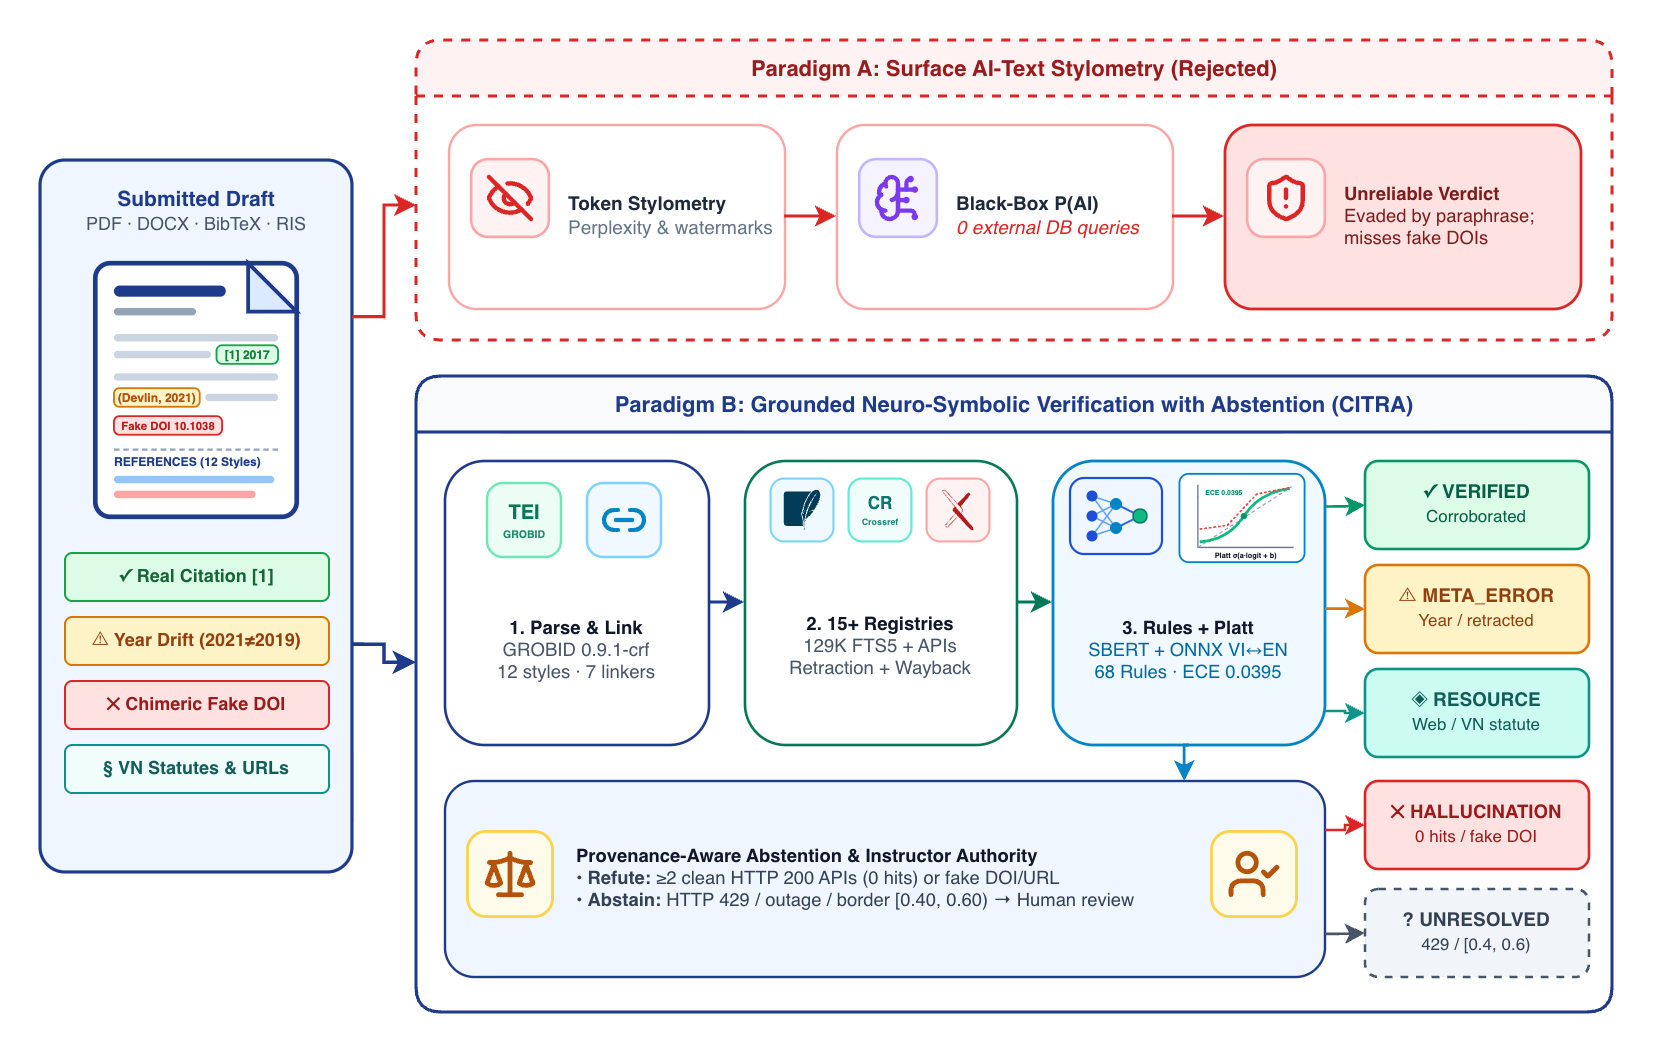
\includegraphics[width=\textwidth,keepaspectratio]{picture/figures/fig2_1_verification_paradigm.png}
    \caption[Comparison between stylistic attribution and external bibliographic verification]{Comparison between stylistic attribution of machine-generated text and external bibliographic verification with provenance-aware abstention.}
    \label{fig:verification-paradigm}
\end{figure}

The second paradigm, \emph{external bibliographic and claim verification}, checks each citation against authoritative registries and compares inline claims against retrieved evidence, following fact-verification frameworks such as FEVER~\cite{thorne2018fever}, SciFact~\cite{wadden2020scifact}, and citation-grounded generation benchmarks such as ALCE~\cite{gao2023alce}. Every flag raised under this paradigm points to concrete external evidence: either multiple live registries confirm that no matching record exists, or a retrieved canonical record exposes a specific metadata or claim discrepancy.

\subsection{Comparison with Existing Systems}

Existing academic integrity platforms, reference managers, and research benchmarks each address only part of the student manuscript verification workflow. Plagiarism checkers such as Turnitin match text overlap against closed repositories but do not detect fabricated references that have zero text overlap with existing literature. Reference managers such as Zotero import clean DOIs for authors but do not audit in-text citation consistency or classroom cohorts. Closed-corpus NLP benchmarks such as SciFact~\cite{wadden2020scifact} verify scientific claims over a fixed set of 5,000 abstracts but do not parse multi-style PDFs or query live registries. Table~\ref{tab:related-work} compares \textbf{CITRA} against five representative system categories across seven technical capabilities.

{\setlength{\tabcolsep}{3.5pt}
\begin{longtable}{|L{0.22}|C{0.11}|C{0.11}|C{0.11}|C{0.12}|C{0.11}|C{0.11}|C{0.11}|}
\caption{Feature comparison between existing tool categories and CITRA (\texttt{v3.90.5}).}\label{tab:related-work}\\
\hline
\textbf{System Category} & \textbf{Multi\-Style PDF} & \textbf{Bipar\-tite Linker} & \textbf{15+ Live APIs} & \textbf{Claim Align.} & \textbf{Safe Abstain} & \textbf{Calib.\ Prob.} & \textbf{VN Legal} \\
\hline
\endfirsthead
\multicolumn{8}{c}{\itshape Table \thetable\ (continued from previous page)}\\
\hline
\textbf{System Category} & \textbf{Multi\-Style PDF} & \textbf{Bipar\-tite Linker} & \textbf{15+ Live APIs} & \textbf{Claim Align.} & \textbf{Safe Abstain} & \textbf{Calib.\ Prob.} & \textbf{VN Legal} \\
\hline
\endhead
\hline
\multicolumn{8}{r}{\itshape Continued on next page}\\
\endfoot
\hline
\endlastfoot
Text Overlap Tools (Turnitin / iThenticate) & Partial & No & No & No & No & No & No \\
\hline
AI Style Detectors (GPTZero / Watermarks) & No & No & No & No & No & Partial & No \\
\hline
Prompt-Only LLM Checkers & Partial & No & Partial & Partial & No & No & No \\
\hline
Reference Managers (Zotero / GROBID) & Yes & No & Partial & No & No & No & No \\
\hline
Claim Benchmarks (SciFact / ALCE) & No & No & No & Yes & Partial & No & No \\
\hline
\textbf{CITRA (\texttt{v3.90.5})} & \textbf{Yes (12)} & \textbf{Yes (8)} & \textbf{Yes (15+)} & \textbf{VI$\leftrightarrow$EN} & \textbf{Yes} & \textbf{Platt} & \textbf{Yes} \\
\hline
\end{longtable}
}

\section{Scholarly Registries and Persistent Identifiers}

\subsection{Federated Bibliographic Sources}

Large-scale bibliometric studies show substantial coverage gaps between individual scholarly databases across disciplines and publication types~\cite{visser2021bibliographic}. Relying on a single API also creates severe rate-limit bottlenecks during classroom submission deadlines. \textbf{CITRA} therefore combines an offline full-text corpus with domain-aware routing across more than fifteen scholarly, technical, and archival registries, as summarized in Table~\ref{tab:sources}.

\begin{longtable}{|L{0.27}|L{0.36}|L{0.37}|}
\caption{Scholarly registries and validators integrated into the CITRA retrieval layer.}\label{tab:sources}\\
\hline
\textbf{Source / Validator} & \textbf{Primary Coverage} & \textbf{Role in Pipeline} \\
\hline
\endfirsthead
\multicolumn{3}{c}{\itshape Table \thetable\ (continued from previous page)}\\
\hline
\textbf{Source / Validator} & \textbf{Primary Coverage} & \textbf{Role in Pipeline} \\
\hline
\endhead
\hline
\multicolumn{3}{r}{\itshape Continued on next page}\\
\endfoot
\hline
\endlastfoot
\textbf{Local Corpus} (\texttt{local\_papers.db}) & \textbf{129,125 records} (128,105 unique papers; 82,877 abstracts) from ACL Anthology~\cite{acl-anthology} and arXiv & \textbf{Tier 0} sub-100\,ms offline SQLite FTS5 BM25 lookup \\
\hline
\textbf{Seminal Whitelist} (\texttt{\_KNOWN\_PAPERS}) & \textbf{101} foundational CS, AI, NLP, and deep learning publications & \textbf{Tier 0} instant lookup for heavily cited canonical papers \\
\hline
\textbf{Crossref}~\cite{crossref-tdm} \& \textbf{Retraction Watch} & Peer-reviewed journals, proceedings, book chapters, and retraction notices & \textbf{Tier 1} DOI resolution, Journal Article Tag Suite (JATS) abstract parsing, and \texttt{is\_retracted} screening \\
\hline
\textbf{OpenAlex}~\cite{openalex} & Global open scholarly graph spanning journals, preprints, and repositories & \textbf{Tier 1} broad metadata lookup and inverted-index abstract reconstruction \\
\hline
\textbf{DataCite}~\cite{datacite} \& \textbf{Global DOI RA}~\cite{doi-handbook} & Zenodo/Figshare/OSF datasets and regional DOI agencies (JaLC, CNKI, KISTI, mEDRA) & \textbf{Tier 1} non-Crossref DOI resolution and \texttt{R-DOI-RA-NO-CSL} safe abstention \\
\hline
\textbf{DOAJ}~\cite{doaj} \& \textbf{OpenAIRE / HAL} & Open-access journals (including regional Asian venues), institutional repositories, and preprints & \textbf{Tier 1} open-access journal and institutional repository verification \\
\hline
\textbf{DBLP}~\cite{dblp} \& \textbf{arXiv API}~\cite{arxiv-api} & Computer science conferences/workshops and STEM preprints & \textbf{Tier 1} domain-routed CS/AI bibliography and exact \texttt{arXiv} ID lookup \\
\hline
\textbf{Europe PMC}~\cite{europepmc} \& \textbf{NCBI / bioRxiv} & PubMed/MEDLINE biomedical, clinical, psychology, and life-science preprints & \textbf{Tier 1} domain-routed life-science lookup and abstract enrichment \\
\hline
\textbf{OpenLibrary}~\cite{openlibrary} \& \textbf{Google Books} & Textbooks, monographs, ISBN metadata, and multi-edition printings & \textbf{Tier 1} book verification and cross-edition year tolerance \\
\hline
\textbf{Hugging Face, IETF RFC, PyPI \& Wikidata} & ML models/datasets, RFC internet standards, Python packages, and OpenCitations & \textbf{Tier 1} software, technical standard, and open citation verification \\
\hline
\textbf{Serper / SerpAPI Router} & Academic web index fallback & \textbf{Tier 2} optional fallback when Tier 0 and Tier 1 return zero candidates \\
\hline
\textbf{HTTP + Wayback} \texttt{Link\allowbreak Validator}~\cite{openlibrary} & Live HTTP/HTTPS targets and Internet Archive CDX snapshots & \textbf{Parallel} URL liveness, Soft-404 HTML metadata, and archive check \\
\hline
\end{longtable}

\subsection{DOI Resolution and Retraction Screening}

A Digital Object Identifier (DOI) provides a persistent handle for scholarly objects~\cite{doi-handbook}, yet syntactic validity (\texttt{10.xxxx/...}) does not guarantee legitimacy. Generative models frequently invent unregistered suffixes under real publisher prefixes (such as \texttt{10.1109/}) or copy a real DOI from a high-profile paper onto a fabricated citation. Conversely, legitimate Asian or European journals registered through agencies such as JaLC, CNKI, KISTI, or mEDRA resolve at \texttt{doi.org/ra/} without exposing metadata in Crossref. Querying the Global DOI Registration Agency API allows \textbf{CITRA} to abstain safely on valid regional DOIs while exposing unregistered and chimeric DOIs. Simultaneously, checking Crossref update-to metadata and Retraction Watch flags prevents retracted articles from passing silently as verified sources.

\section{Theoretical Foundations}

\subsection{Lexical and Semantic Title Similarity}

Bibliographic strings vary across citation styles due to subtitle truncation, punctuation differences, hyphenation, and edition markers. \textbf{CITRA} therefore combines lexical string similarity with dense neural embeddings. At the lexical level, RapidFuzz computes token-set ratios (insensitive to word reordering), normalized Levenshtein ratios (sensitive to character typos), and guarded prefix ratios (handling omitted subtitles after colons). At the semantic level, titles are encoded into 384-dimensional vectors using the Transformer architecture~\cite{vaswani2017} distilled via BERT~\cite{bert} and MiniLM~\cite{wang2020minilm} into the Sentence-BERT checkpoint \texttt{all-MiniLM-L6-v2}~\cite{reimers2019sbert}. When Vietnamese prose cites an English source, \textbf{CITRA} activates a quantized ONNX INT8 multilingual encoder (\texttt{paraphrase-multilingual-MiniLM-L12-v2}) trained via multilingual knowledge distillation~\cite{reimers2020multilingual}.

\subsection{Multi-Sentence Context Alignment}

Checking bibliography metadata alone cannot catch \emph{contextual misattribution}, where a student cites a real paper to support an unrelated or opposite claim. However, comparing a single in-text sentence directly against an entire ten-sentence abstract suffers from length dilution because background and conclusion sentences wash out the specific sentence being cited. Given an in-text citation context $c$ and a candidate abstract $A$ segmented into sentences $\{s_1, \dots, s_m\}$, \textbf{CITRA} computes the pooled abstract alignment score $s_{\text{abs}}(c, A)$ defined in Equation~\eqref{eq:abs-pooling}:
\begin{equation}\label{eq:abs-pooling}
s_{\text{abs}}(c, A) = \max\Bigl(\cos\bigl(\mathbf{e}(c), \mathbf{e}(A)\bigr),\; 0.65 \max_{1 \le i \le m} \cos\bigl(\mathbf{e}(c), \mathbf{e}(s_i)\bigr) + 0.35 \cos\bigl(\mathbf{e}(c), \mathbf{e}(A)\bigr)\Bigr),
\end{equation}
where $\mathbf{e}(\cdot)$ denotes the L2-normalized sentence embedding. Equation~\eqref{eq:abs-pooling} preserves high similarity when a citation targets a single specific finding while retaining whole-abstract context when a citation summarizes the overall paper. The final content alignment combines title similarity ($0.30$), pooled abstract similarity ($0.50$), and full-text snippet similarity ($0.20$, renormalized when full text is absent).

\subsection{Selective Classification and Logit-Space Platt Calibration}

In high-stakes decision support, a classifier must know when to abstain~\cite{chow1970optimum}, \cite{Geifman2017}, and its reported confidence $p$ must match empirical accuracy~\cite{hand2009}, \cite{guo2017}. Static rule confidences cluster at discrete constants and overestimate certainty near decision boundaries. Given the symbolic verdict class $y_{\text{sym}}$ and the 16-dimensional feature vector $\mathbf{x} \in \mathbb{R}^{16}$, \textbf{CITRA} blends the symbolic rule confidence $C_{\text{sym}}$ with the predicted class probability $P_{\text{ML}}(y_{\text{sym}} \mid \mathbf{x})$ of a Multinomial Logistic Regression model using weight $\alpha \in [0, 1]$, as defined in Equation~\eqref{eq:platt-calib}:
\begin{equation}\label{eq:platt-calib}
p_{\text{blend}} = \alpha C_{\text{sym}} + (1 - \alpha) P_{\text{ML}}(y_{\text{sym}} \mid \mathbf{x}), \;\;
P_{\text{cal}} = \operatorname{clip}\!\left(\sigma\Bigl(a \cdot \ln\frac{\tilde{p}}{1 - \tilde{p}} + b\Bigr),\, 0.01,\, 0.99\right),
\end{equation}
where $\tilde{p} = \min(\max(p_{\text{blend}}, 10^{-4}), 1 - 10^{-4})$ prevents numerical overflow at $0$ or $1$, $\sigma(z) = (1 + e^{-z})^{-1}$ is the logistic sigmoid, and $(a, b)$ are scalar Platt scaling parameters~\cite{platt1999} fitted on a disjoint validation split by minimizing a joint negative log-likelihood and Brier score objective~\cite{brier1950}.

\subsection{Paper-Disjoint Evaluation Design}

Following Empirical Software Engineering experimentation guidelines~\cite{wohlin2012experimentation} and claim-verification benchmarks~\cite{thorne2018fever}, \cite{wadden2020scifact}, training and evaluating a hybrid verifier requires strict protection against data leakage and dataset artifacts~\cite{gururangan2018annotation}, \cite{poliak2018hypothesis}. If perturbed variants of the same base paper appear in both training and testing splits, a classifier can memorize paper-level feature distributions. Similarly, if non-zero semantic context scores appear only in verified examples, the model learns a trivial shortcut. All quantitative experiments in Chapter~\ref{chap:results} therefore partition base papers strictly before perturbation, retain real Sentence-BERT encodings across all classes without artificial clamping, and evaluate hypotheses using continuity-corrected McNemar tests~\cite{dietterich1998approximate}, Holm--Bonferroni multiple-comparison adjustments~\cite{holm1979simple}, and paired bootstrap resampling~\cite{bergkirkpatrick2012empirical}, \cite{dror2018hitchhiker}.

\section{Chapter Summary}

This chapter reviewed the literature on PDF citation parsing, probabilistic record linkage, and hallucinated reference detection, and contrasted \textbf{CITRA} against five categories of existing tools. It also established the multi-registry retrieval rationale and the mathematical formulations for sentence-pooled semantic alignment and logit-space Platt calibration. Chapter~\ref{chap:overview} translates these foundations into formal software requirements, use cases, database schemas, and deployment specifications.


\newpage
\chapter{System Analysis and Design}
\label{chap:overview}

\section{Requirements Engineering}

System requirements were elicited from university capstone project supervision workflows and structured according to IEEE Std 29148-2018~\cite{ieee29148} for functional specifications and ISO/IEC 25010:2023~\cite{iso25010} for software product quality attributes.

\subsection{Functional Requirements}

Every functional requirement is specified as an atomic, testable obligation assigned to an explicit actor and priority level (\textbf{Must} or \textbf{Should}). Table~\ref{tab:func-reqs} lists the sixteen core functional requirements grouped across five functional subsystems.

{\setlength{\tabcolsep}{3.5pt}
\begin{longtable}{|C{0.10}|L{0.15}|L{0.39}|C{0.11}|L{0.25}|}
\caption{Atomic functional requirements organized by subsystem (IEEE 29148).}\label{tab:func-reqs}\\
\hline
\textbf{ID} & \textbf{Actor} & \textbf{Requirement Specification} & \textbf{Prio.} & \textbf{Acceptance Criterion} \\
\hline
\endfirsthead
\multicolumn{5}{c}{\itshape Table \thetable\ (continued from previous page)}\\
\hline
\textbf{ID} & \textbf{Actor} & \textbf{Requirement Specification} & \textbf{Prio.} & \textbf{Acceptance Criterion} \\
\hline
\endhead
\hline
\multicolumn{5}{r}{\itshape Continued on next page}\\
\endfoot
\hline
\endlastfoot
\multicolumn{5}{|l|}{\textbf{Subsystem 1: Identity, Session Management, and Access Control}} \\
\hline
\textbf{\texttt{FR-01}} & Guest / Student & The system shall register accounts, verify one-time email activation and password-reset tokens, and authenticate sessions via local credentials or Google OAuth2. & \textbf{Must} & Invalid/expired token rejected; revoked JWT returns \textbf{HTTP 401}. \\
\hline
\textbf{\texttt{FR-02}} & All Roles & The system shall enforce Role-Based Access Control (\texttt{user}, \texttt{teacher}, \texttt{admin}), personal API keys, and cross-user ownership checks on every resource. & \textbf{Must} & Cross-user essay/verdict access returns \textbf{HTTP 403} (zero IDOR). \\
\hline
\multicolumn{5}{|l|}{\textbf{Subsystem 2: Document Ingestion, Parsing, and Bidirectional Linking}} \\
\hline
\textbf{\texttt{FR-03}} & Student / Teacher & The system shall accept single and batch manuscript uploads in PDF, DOCX, BibTeX, and RIS formats after validating magic bytes, file size, page count, and monthly quota. & \textbf{Must} & Disguised non-PDF/DOCX or over-quota upload rejected cleanly. \\
\hline
\textbf{\texttt{FR-04}} & Student / Teacher & The system shall stream real-time progress across eight pipeline stages and refund upload quota automatically if an asynchronous job fails permanently. & \textbf{Must} & SSE emits steps 0--7; crashed job refunds quota atomically. \\
\hline
\textbf{\texttt{FR-05}} & Pipeline & The system shall segment uploaded manuscripts into body text, in-text markers with surrounding context, and bibliography entries across 12 citation styles (including Vietnamese laws). & \textbf{Must} & \textbf{$\ge 97\%$} bibliography detection on 310-PDF multi-style suite. \\
\hline
\textbf{\texttt{FR-06}} & Pipeline & The system shall detect scanned or legacy-encoded Vietnamese PDFs and invoke selective Optical Character Recognition (OCR) or encoding normalization. & Should & Scanned pages recorded in document diagnostics metadata. \\
\hline
\textbf{\texttt{FR-07}} & Pipeline & The system shall link every in-text citation marker to its target bibliography entry and classify each edge into one of eight structural mapping statuses. & \textbf{Must} & Orphans, uncited refs, and year mismatches isolated accurately. \\
\hline
\multicolumn{5}{|l|}{\textbf{Subsystem 3: Federated Retrieval and Identifier Validation}} \\
\hline
\textbf{\texttt{FR-08}} & Pipeline & The system shall query the offline scholarly corpus and live registries by domain, recording per-source success, failure, and rate-limit provenance. & \textbf{Must} & Offline recall \textbf{$\ge 99\%$}; \textbf{HTTP 429} distinguished from 0 hits. \\
\hline
\textbf{\texttt{FR-09}} & Pipeline & The system shall validate cited URLs and DOIs against SSRF-safe HTTP probes, Retraction Watch metadata, and Internet Archive snapshots. & \textbf{Must} & Private IP targets blocked; retracted works flagged \textbf{$100\%$}. \\
\hline
\multicolumn{5}{|l|}{\textbf{Subsystem 4: Neuro-Symbolic Verification, Scoring, and Remediation}} \\
\hline
\textbf{\texttt{FR-10}} & Pipeline & The system shall compute lexical, semantic, and cross-lingual (\texttt{VI}$\leftrightarrow$\texttt{EN}) alignment between in-text claims and retrieved source titles/abstracts. & \textbf{Must} & Contradicted claims and cross-lingual matches scored in $[0,1]$. \\
\hline
\textbf{\texttt{FR-11}} & Pipeline & The system shall assign one of five verdict labels, a Platt-calibrated probability, and an ordered list of triggered symbolic rule IDs to each reference. & \textbf{Must} & Test accuracy \textbf{$\ge 98.5\%$}, \textbf{$\text{ECE} \le 0.05$}, \textbf{$100\%$} rule trace. \\
\hline
\textbf{\texttt{FR-12}} & Pipeline & The system shall calculate the five-component Citation Integrity Score (CIS) in $[0, 100]$ and generate bilingual (\texttt{EN}/\texttt{VI}) explanations. & \textbf{Must} & Component weights sum to $1.00$; explanations render in EN \& VI. \\
\hline
\textbf{\texttt{FR-13}} & Student / Teacher & The system shall export sanitized reports (PDF, DOCX, CSV, JSON) and generate repaired bibliographies in APA, IEEE, TDTU, BibTeX, RIS, and DOCX formats. & Should & Repaired entries reflect canonical registry metadata without macros. \\
\hline
\textbf{\texttt{FR-14}} & Student / Public & The system shall issue time-limited cryptographic share links with QR verification receipts for read-only third-party inspection. & Should & Expired or tampered share token returns \textbf{HTTP 404/403}. \\
\hline
\multicolumn{5}{|l|}{\textbf{Subsystem 5: Classroom Cohort Supervision and Platform Administration}} \\
\hline
\textbf{\texttt{FR-15}} & Teacher & The system shall allow teachers to manage classes via join codes, inspect cohort analytics and shared hallucinations, and override verdicts when override permission is granted. & \textbf{Must} & Override updates verdict, recalculates CIS, and logs audit entry. \\
\hline
\textbf{\texttt{FR-16}} & Admin & The system shall allow administrators to manage accounts, promo codes, cache state, upstream circuit breakers, and audit logs. & \textbf{Must} & Circuit-breaker reset and cache clear take effect immediately. \\
\hline
\end{longtable}
}

\subsection{Non-Functional Requirements}

To ensure production readiness on standard university hardware without GPUs, ten quantitative Non-Functional Requirements (NFRs) are mapped to ISO/IEC 25010:2023 quality categories in Table~\ref{tab:nfr-reqs}.

{\setlength{\tabcolsep}{3.5pt}
\begin{longtable}{|C{0.11}|L{0.25}|L{0.40}|L{0.24}|}
\caption{Quantitative non-functional requirements mapped to ISO/IEC 25010:2023.}\label{tab:nfr-reqs}\\
\hline
\textbf{ID} & \textbf{ISO/IEC 25010 Attribute} & \textbf{Quality Requirement} & \textbf{Target Metric / SLA} \\
\hline
\endfirsthead
\multicolumn{4}{c}{\itshape Table \thetable\ (continued from previous page)}\\
\hline
\textbf{ID} & \textbf{ISO/IEC 25010 Attribute} & \textbf{Quality Requirement} & \textbf{Target Metric / SLA} \\
\hline
\endhead
\hline
\multicolumn{4}{r}{\itshape Continued on next page}\\
\endfoot
\hline
\endlastfoot
\textbf{\texttt{NFR-01}} & \textbf{Performance Efficiency} (Time Behaviour) & Warm-cache verification latency for a 50-page capstone report ($\sim$32 references) on CPU hardware. & \textbf{$P_{90} \le 2.5\text{\,s}$} (cold Wide Area Network [WAN] $\le 15\text{\,s}$). \\
\hline
\textbf{\texttt{NFR-02}} & \textbf{Performance Efficiency} (Resource Utilization) & Peak backend Python Resident Set Size (RSS) during a 150-page monograph analysis. & \textbf{$\text{RSS} \le 1.5\text{\,GB}$}; heap $\Delta \le 25\text{\,MB}$. \\
\hline
\textbf{\texttt{NFR-03}} & \textbf{Performance Efficiency} (Capacity) & Simultaneous classroom deadline uploads handled without SQLite lock errors or HTTP 5xx responses. & \textbf{$50$ concurrent uploads, $0\%$ failure}. \\
\hline
\textbf{\texttt{NFR-04}} & \textbf{Reliability} (Fault Tolerance) & Graceful degradation when GROBID or upstream scholarly APIs time out or return HTTP 429. & Automatic PyMuPDF fallback; \textbf{$100\%$ safe abstention} on 429. \\
\hline
\textbf{\texttt{NFR-05}} & \textbf{Functional Suitability} & Zero false hallucination accusations on verified works and well-calibrated confidence probabilities. & False hall.\ \textbf{$\le 0.1\%$}; \textbf{$\text{ECE} \le 0.05$}. \\
\hline
\textbf{\texttt{NFR-06}} & \textbf{Security} (Confidentiality \& Integrity) & Protection against SSRF, IDOR, cross-site scripting, CSV formula injection, and brute-force login. & \textbf{Pinned-IP SSRF block}; salted \texttt{bcrypt} + SHA-256/HMAC tokens. \\
\hline
\textbf{\texttt{NFR-07}} & \textbf{Interaction Capability} (Usability) & Accessible Light and Dark editorial interfaces with progressive disclosure and bilingual localization. & \textbf{WCAG 2.1 AA} ($\ge 4.5:1$ contrast); $0\text{\,px}$ overflow. \\
\hline
\textbf{\texttt{NFR-08}} & \textbf{Performance Efficiency} (Time \& Resource) & Code-split frontend JavaScript delivery for fast initial page rendering over campus networks. & Initial entry chunk \textbf{$\le 250\text{\,kB}$} ($\le 80\text{\,kB}$ gzip). \\
\hline
\textbf{\texttt{NFR-09}} & \textbf{Maintainability} (Modularity \& Testability) & Acyclic 8-layer Python architecture and automated backend, frontend, and browser regression suites. & \textbf{$\ge 2{,}500$} automated tests, $0$ failures. \\
\hline
\textbf{\texttt{NFR-10}} & \textbf{Portability} (Installability \& Replaceability) & Reproducible containerized deployment across Linux and macOS CPU hosts without proprietary GPUs. & 3-container health ready \textbf{$\le 60\text{\,s}$}; $0$ GPU dependencies. \\
\hline
\end{longtable}
}

\section{Actors, Access Control, and Use Case Specifications}

\subsection{Role-Based Access Control and Capability Gate}

\textbf{CITRA} serves three primary human actors (\textbf{Student} [\texttt{user}], \textbf{Teacher} [\texttt{teacher}], and \textbf{Administrator} [\texttt{admin}]) alongside external parsing and scholarly registries, as modeled in the UML 2.5 Use Case diagram in Figure~\ref{fig:roles}. Authorization is enforced by reusable FastAPI dependency guards rather than ad-hoc conditionals inside route handlers.

\begin{figure}[H]
    \centering
    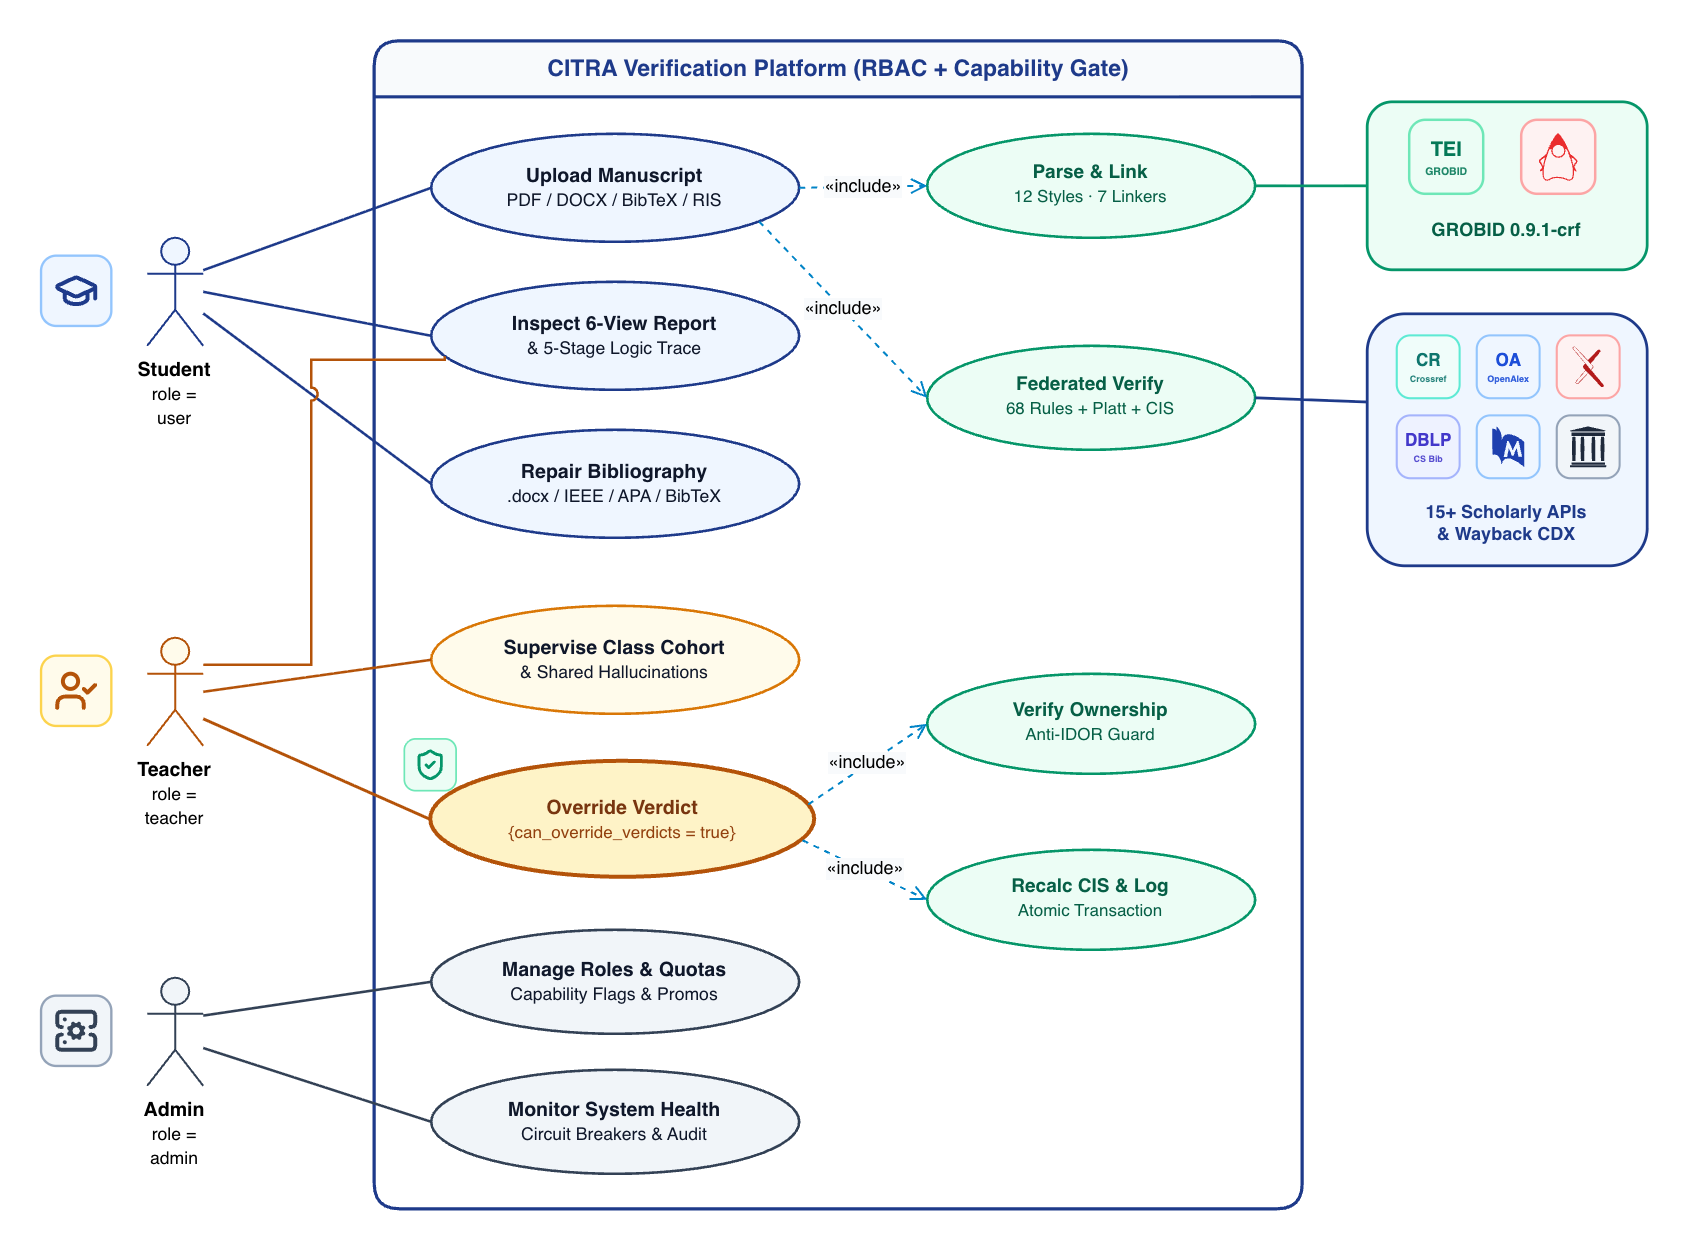
\includegraphics[width=\textwidth,keepaspectratio]{picture/figures/fig3_1_roles.png}
    \caption[UML 2.5 Use Case diagram and RBAC capability gate]{UML 2.5 Use Case diagram across Student, Teacher, and Administrator roles, highlighting the independent \texttt{\{can\_override\_verdicts = true\}} capability guard.}
    \label{fig:roles}
\end{figure}

Crucially, verdict adjudication separates role membership from override authority via an independent boolean column \texttt{users.can\_override\_verdicts}. A faculty member may grant a teaching assistant the \texttt{teacher} role so they can view cohort submissions and triage the pending-review queue, while keeping \texttt{can\_override\_verdicts = False} so only the lead supervisor can reverse a \texttt{suspected\_hallucination} verdict.

\subsection{Core Use Case Specifications}

Table~\ref{tab:uc01}, Table~\ref{tab:uc02}, Table~\ref{tab:uc03}, Table~\ref{tab:uc04}, and Table~\ref{tab:uc05} specify the five primary use cases governing manuscript verification, bibliography repair, instructor adjudication, cohort supervision, and platform administration.

\begin{longtable}{|L{0.24}|L{0.76}|}
\caption{Use Case Specification UC-01: Upload Manuscript and Stream Verification.}\label{tab:uc01}\\
\hline
\textbf{Field} & \textbf{Specification} \\
\hline
\endfirsthead
\multicolumn{2}{c}{\itshape Table \thetable\ (continued from previous page)}\\
\hline
\textbf{Field} & \textbf{Specification} \\
\hline
\endhead
\hline
\multicolumn{2}{r}{\itshape Continued on next page}\\
\endfoot
\hline
\endlastfoot
\textbf{Use Case ID \& Name} & \textbf{UC-01:} Upload Manuscript and Stream Verification (\texttt{FR-03}--\texttt{FR-12}) \\
\hline
\textbf{Primary Actor} & Student (\texttt{user}) or Teacher (\texttt{teacher}) \\
\hline
\textbf{Preconditions} & Actor is authenticated with an active session and remaining monthly upload quota $\ge 1$. \\
\hline
\textbf{Postconditions} & \texttt{essays}, \texttt{citations}, and \texttt{verdicts} rows are persisted; CIS and style profile are stored. \\
\hline
\textbf{Main Success Scenario} & \textbf{1.} Actor selects a \texttt{.pdf}, \texttt{.docx}, \texttt{.bib}, or \texttt{.ris} file (optionally choosing an enrolled class). \newline \textbf{2.} Backend validates magic bytes, size, page limit, and atomically decrements quota via Compare-And-Swap (CAS). \newline \textbf{3.} Backend persists \texttt{EssayRecord(job\_status='queued')} and enqueues the job in \texttt{PipelineAdmissionController}. \newline \textbf{4.} Client subscribes to \texttt{GET /api/essays/\{id\}/events} (SSE) and renders stages 0--7 in real time. \newline \textbf{5.} Worker completes extraction, linking, retrieval, matching, symbolic/ML checking, and CIS scoring, marking \texttt{job\_status='completed'}. \newline \textbf{6.} Client navigates to \texttt{/verification/report/\{id\}}. \\
\hline
\textbf{Alternative / Exception Flows} & \textbf{2a. Invalid MIME or magic bytes:} Backend returns HTTP 400; quota is untouched. \newline \textbf{2b. Quota exhausted:} Backend returns HTTP 402/429; UI displays plan upgrade modal. \newline \textbf{5a. GROBID or external API timeout:} Pipeline switches to PyMuPDF fallback or emits \texttt{R-RATE-LIMITED-ABSTAIN} (\texttt{unresolved}) without failing the job. \newline \textbf{5b. Unrecoverable worker crash:} Stale-job recovery marks \texttt{failed} and refunds 1 quota unit via CAS. \\
\hline
\end{longtable}

\begin{longtable}{|L{0.24}|L{0.76}|}
\caption{Use Case Specification UC-02: Repair Bibliography and Export Manuscript.}\label{tab:uc02}\\
\hline
\textbf{Field} & \textbf{Specification} \\
\hline
\endfirsthead
\multicolumn{2}{c}{\itshape Table \thetable\ (continued from previous page)}\\
\hline
\textbf{Field} & \textbf{Specification} \\
\hline
\endhead
\hline
\multicolumn{2}{r}{\itshape Continued on next page}\\
\endfoot
\hline
\endlastfoot
\textbf{Use Case ID \& Name} & \textbf{UC-02:} Repair Bibliography and Export Manuscript (\texttt{FR-13}) \\
\hline
\textbf{Primary Actor} & Student (\texttt{user}) or Teacher (\texttt{teacher}) \\
\hline
\textbf{Preconditions} & Target essay belongs to Actor (or Actor's supervised class) and \texttt{job\_status='completed'}. \\
\hline
\textbf{Postconditions} & Formatted bibliography strings or repaired \texttt{.docx} / report files are downloaded cleanly. \\
\hline
\textbf{Main Success Scenario} & \textbf{1.} Actor clicks \textit{Fix \& Format Citations} on the report header. \newline \textbf{2.} Backend (\texttt{GET /api/essays/\{id\}/remediate}) maps verified and metadata-erroneous citations to canonical registry fields while isolating \texttt{suspected\_hallucination} entries for manual removal. \newline \textbf{3.} Actor selects target style (\texttt{APA 7th}, \texttt{IEEE}, \texttt{TDTU}, \texttt{BibTeX}, or \texttt{RIS}) and previews field-level diffs. \newline \textbf{4.} Actor downloads the repaired \texttt{.docx} manuscript or sanitized PDF/CSV/JSON audit report. \\
\hline
\textbf{Alternative / Exception Flows} & \textbf{2a. Citation is suspected hallucination:} System refuses to fabricate replacement metadata and marks entry \texttt{hallucination} for author deletion. \\
\hline
\end{longtable}

\begin{longtable}{|L{0.24}|L{0.76}|}
\caption{Use Case Specification UC-03: Adjudicate and Override Citation Verdict.}\label{tab:uc03}\\
\hline
\textbf{Field} & \textbf{Specification} \\
\hline
\endfirsthead
\multicolumn{2}{c}{\itshape Table \thetable\ (continued from previous page)}\\
\hline
\textbf{Field} & \textbf{Specification} \\
\hline
\endhead
\hline
\multicolumn{2}{r}{\itshape Continued on next page}\\
\endfoot
\hline
\endlastfoot
\textbf{Use Case ID \& Name} & \textbf{UC-03:} Adjudicate and Override Citation Verdict (\texttt{FR-15}) \\
\hline
\textbf{Primary Actor} & Teacher (\texttt{teacher}) or Administrator (\texttt{admin}) with \texttt{can\_override\_verdicts = True} \\
\hline
\textbf{Preconditions} & Essay belongs to a class owned by Teacher (or Actor is Admin); target verdict belongs to that essay. \\
\hline
\textbf{Postconditions} & Verdict label updated, essay CIS recomputed, and \texttt{audit\_logs} row inserted in one transaction. \\
\hline
\textbf{Main Success Scenario} & \textbf{1.} Teacher inspects a flagged citation in the Reference Inspector or Pending Reviews queue. \newline \textbf{2.} Teacher selects a new verdict label (e.g.\ \texttt{verified}) and enters a written justification note. \newline \textbf{3.} Backend (\texttt{POST /api/essays/\{id\}/verdicts/\{vid\}/override}) verifies RBAC, capability flag, and essay-to-verdict ownership. \newline \textbf{4.} Within a single DB transaction, backend updates \texttt{VerdictRecord}, re-runs \texttt{CISCalculator.compute()}, updates \texttt{EssayRecord.cis\_json}, and inserts an \texttt{AuditLog} entry. \newline \textbf{5.} UI refreshes the CIS score ring and displays the override badge. \\
\hline
\textbf{Alternative / Exception Flows} & \textbf{3a. Capability flag is False:} Backend aborts with HTTP 403 Forbidden. \newline \textbf{3b. Verdict ID belongs to another essay (IDOR attempt):} Backend aborts with HTTP 404/403. \\
\hline
\end{longtable}

\begin{longtable}{|L{0.24}|L{0.76}|}
\caption{Use Case Specification UC-04: Supervise Classroom Cohort and Shared Anomalies.}\label{tab:uc04}\\
\hline
\textbf{Field} & \textbf{Specification} \\
\hline
\endfirsthead
\multicolumn{2}{c}{\itshape Table \thetable\ (continued from previous page)}\\
\hline
\textbf{Field} & \textbf{Specification} \\
\hline
\endhead
\hline
\multicolumn{2}{r}{\itshape Continued on next page}\\
\endfoot
\hline
\endlastfoot
\textbf{Use Case ID \& Name} & \textbf{UC-04:} Supervise Classroom Cohort and Shared Anomalies (\texttt{FR-15}) \\
\hline
\textbf{Primary Actor} & Teacher (\texttt{teacher}) \\
\hline
\textbf{Preconditions} & Teacher is authenticated and owns at least one classroom cohort. \\
\hline
\textbf{Postconditions} & Cohort analytics, shared hallucination clusters, and ZIP/CSV gradebooks are generated. \\
\hline
\textbf{Main Success Scenario} & \textbf{1.} Teacher creates a class and shares the generated \texttt{join\_code} (default format \texttt{CITRA-XXXX}) with students. \newline \textbf{2.} Students enroll via \texttt{POST /api/teacher/classes/join} and attach project report uploads to the class. \newline \textbf{3.} Teacher opens \texttt{/teacher/classes/\{classId\}}; backend aggregates cohort CIS bands, 5-year citation recency, top triggered rules, and identical fabricated citations appearing across multiple students. \newline \textbf{4.} Teacher exports sanitized CSV summary or bulk ZIP archive of cohort reports. \\
\hline
\textbf{Alternative / Exception Flows} & \textbf{2a. Compromised join code:} Teacher regenerates \texttt{join\_code} without dropping existing members. \\
\hline
\end{longtable}

\begin{longtable}{|L{0.24}|L{0.76}|}
\caption{Use Case Specification UC-05: Monitor System Telemetry and Reset Circuit Breakers.}\label{tab:uc05}\\
\hline
\textbf{Field} & \textbf{Specification} \\
\hline
\endfirsthead
\multicolumn{2}{c}{\itshape Table \thetable\ (continued from previous page)}\\
\hline
\textbf{Field} & \textbf{Specification} \\
\hline
\endhead
\hline
\multicolumn{2}{r}{\itshape Continued on next page}\\
\endfoot
\hline
\endlastfoot
\textbf{Use Case ID \& Name} & \textbf{UC-05:} Monitor System Telemetry and Reset Circuit Breakers (\texttt{FR-16}) \\
\hline
\textbf{Primary Actor} & Administrator (\texttt{admin}) \\
\hline
\textbf{Preconditions} & Actor is authenticated with \texttt{role = 'admin'}. \\
\hline
\textbf{Postconditions} & Upstream provider circuit breakers or expired cache entries are safely reset; telemetry is refreshed. \\
\hline
\textbf{Main Success Scenario} & \textbf{1.} Admin navigates to \texttt{/admin/system}. \newline \textbf{2.} Backend (\texttt{GET /api/system/health}) reports GROBID readiness, SQLite WAL statistics, cache hit rates, verdict distributions, and per-provider circuit-breaker states (\texttt{closed}, \texttt{half\_open}, \texttt{open}). \newline \textbf{3.} After an external API outage resolves, Admin triggers \texttt{POST /api/system/circuit-breakers/reset} to restore live traffic immediately. \\
\hline
\textbf{Alternative / Exception Flows} & \textbf{2a. GROBID container unreachable:} Health monitor marks parser \texttt{degraded (regex fallback)} while keeping uploads operational. \\
\hline
\end{longtable}

\section{End-to-End Processing and Concurrency Design}

\subsection{Eight-Stage Verification Sequence}

Figure~\ref{fig:workflow} presents the UML 2.5 Sequence Diagram for asynchronous manuscript verification and transactional instructor adjudication. Unlike synchronous request-response pipelines that block HTTP workers and time out on 100-page capstone reports, \textbf{CITRA} decouples upload ingestion from background execution across eight tracked pipeline stages: (0) \texttt{parsing}, (1) \texttt{style\_detection}, (2) \texttt{extracting}, (3) \texttt{linking}, (4) \texttt{retrieving}, (5) \texttt{comparing}, (6) \texttt{checking}, and (7) \texttt{scoring}. At each stage boundary, a thread-safe \texttt{ProgressTracker} publishes structured snapshots over Server-Sent Events (SSE) with automatic time-to-live (TTL) eviction once the client disconnects.

\begin{figure}[H]
    \centering
    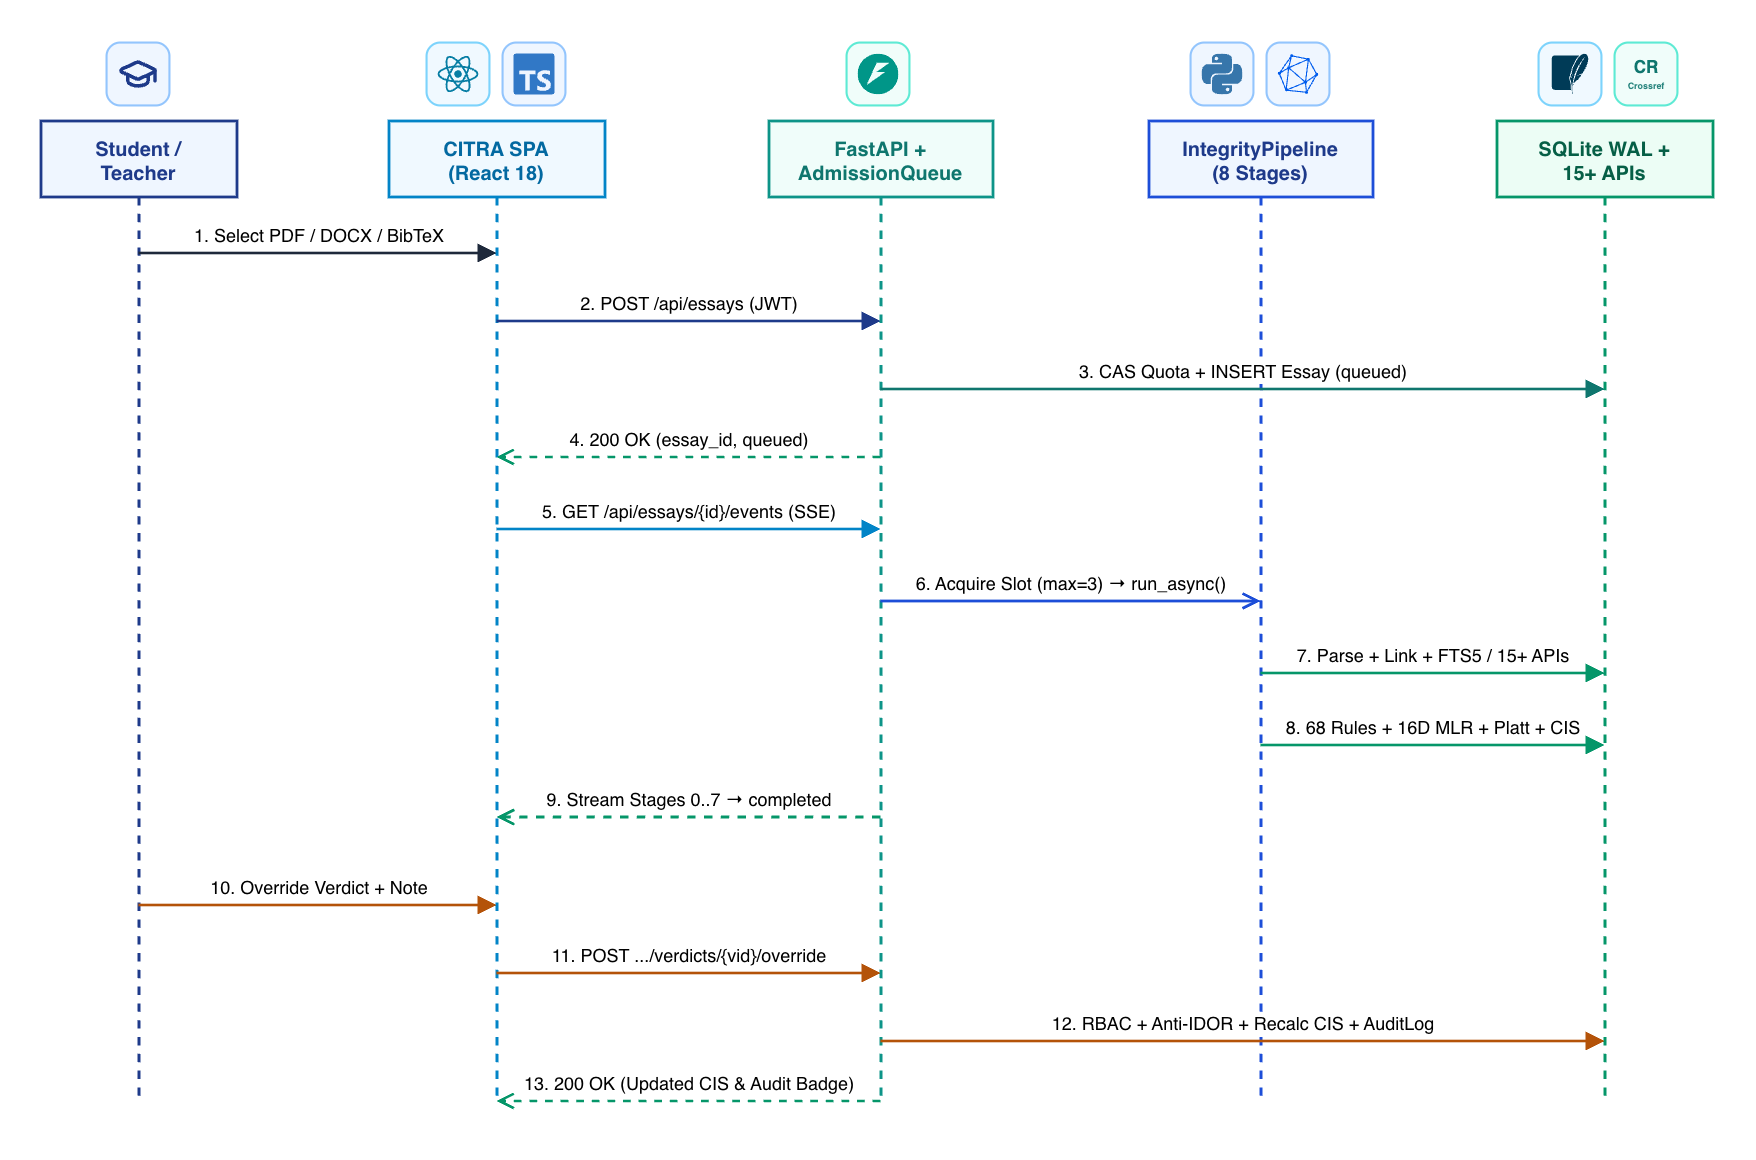
\includegraphics[width=\textwidth,keepaspectratio]{picture/figures/fig3_2_workflow.png}
    \caption[UML 2.5 Sequence diagram for asynchronous verification and teacher override]{UML 2.5 Sequence diagram illustrating asynchronous eight-stage SSE verification and transactional teacher verdict override.}
    \label{fig:workflow}
\end{figure}

\subsection{Admission Control, Worker Modes, and Crash Recovery}

During final submission deadlines, dozens of students may upload project reports simultaneously. Running unbounded Sentence-BERT and GROBID tasks concurrently would exhaust host RAM. \textbf{CITRA} prevents overload through \texttt{PipelineAdmissionController} (\texttt{api/progress.py}), which coordinates slot admission via a thread lock and per-waiter \texttt{asyncio.Event} FIFO queue (\texttt{max\_concurrent = 3} active workers by default) while reporting live \texttt{queue\_position} updates to waiting browsers.

The runtime supports three deployment modes via \texttt{CITRA\_WORKER\_MODE}: \texttt{inline} (single-container FastAPI + background worker), \texttt{web\_only} (API nodes enqueue jobs into SQLite), and \texttt{worker\_only} (dedicated background consumer polling queued jobs with 30-second \texttt{job\_heartbeat\_at} updates). To guarantee crash resilience, \texttt{api/job\_recovery.py} scans for orphaned \texttt{queued} or \texttt{processing} jobs on startup: interrupted jobs below \texttt{MAX\_ORPHAN\_RECOVERY\_ATTEMPTS = 2} are safely re-queued, whereas permanently failed jobs transition to \texttt{failed} and atomically refund the user's monthly upload quota via a Compare-And-Swap (\texttt{quota\_charged: 1 $\rightarrow$ 0}) SQL update so a user is never double-refunded or unfairly billed.

\section{Persistent Data Model and Storage Architecture}

\subsection{Relational Schema and Local FTS5 Corpus}

The persistence layer comprises \textbf{fifteen SQLAlchemy ORM tables} in the primary application database (\texttt{data/app.db}) alongside the read-mostly offline scholarly corpus (\texttt{data/local\_papers.db}, 129,125 records indexed via SQLite FTS5), as summarized in Table~\ref{tab:data-model} and depicted in the Crow's Foot Entity-Relationship Diagram (ERD) in Figure~\ref{fig:data-model}. Public verification share links (\texttt{FR-14}) are issued as stateless HMAC-SHA256 signed tokens (\texttt{sh\_\{eid\}\_\{exp\}\_\{sig\}}) rather than requiring mutable share-session rows.

{\setlength{\tabcolsep}{3.5pt}
\begin{longtable}{|L{0.25}|L{0.46}|L{0.29}|}
\caption{Persistent SQLAlchemy ORM entities in \texttt{db/models.py} (\texttt{v3.90.5}).}\label{tab:data-model}\\
\hline
\textbf{Table Name} & \textbf{Principal Columns and Responsibility} & \textbf{Relationships \& Keys} \\
\hline
\endfirsthead
\multicolumn{3}{c}{\itshape Table \thetable\ (continued from previous page)}\\
\hline
\textbf{Table Name} & \textbf{Principal Columns and Responsibility} & \textbf{Relationships \& Keys} \\
\hline
\endhead
\hline
\multicolumn{3}{r}{\itshape Continued on next page}\\
\endfoot
\hline
\endlastfoot
\textbf{\texttt{users}} & Credentials, OAuth link, \texttt{role}, \texttt{can\_override\_verdicts}, \texttt{plan\_tier}, quota counters, \texttt{created\_at}, \texttt{last\_login\_at} & \textbf{1-to-N} with essays, sessions, tokens, classes, memberships, API keys \\
\hline
\textbf{\texttt{sessions}} & Active bearer \texttt{token} string, \texttt{created\_at}, \texttt{expires\_at} & \textbf{N-to-1} \texttt{users}; revoked on logout or password change \\
\hline
\textbf{\texttt{auth\_tokens}} & One-time SHA-256 \texttt{token\_hash} digests for email activation and password reset & \textbf{N-to-1} \texttt{users}; indexed on \texttt{token\_hash} \\
\hline
\textbf{\texttt{api\_keys}} & \texttt{name}, \texttt{key\_prefix}, SHA-256 \texttt{key\_hash}, \texttt{created\_at}, \texttt{last\_used\_at}, \texttt{is\_active} & \textbf{N-to-1} \texttt{users}; programmatic CLI/API access \\
\hline
\textbf{\texttt{essays}} & \texttt{filename}, \texttt{num\_pages}, \texttt{job\_status}, \texttt{job\_attempt\_count}, \texttt{job\_heartbeat\_at}, \texttt{quota\_charged}, \texttt{style\_profile\_json}, \texttt{cis\_json} & \textbf{N-to-1} \texttt{users} \& optional \texttt{classes}; \textbf{1-to-N} citations, verdicts \\
\hline
\textbf{\texttt{citations}} & Extracted \texttt{in\_text} / \texttt{reference\_list} text, parsed fields, surrounding \texttt{context}, \texttt{mapping\_status}, \texttt{citation\_link\_json} & \textbf{N-to-1} \texttt{essays} (cascade delete) \\
\hline
\textbf{\texttt{verdicts}} & Five-class \texttt{label}, calibrated \texttt{confidence}, \texttt{triggered\_rules}, \texttt{mismatched\_fields}, \texttt{features} JSON, override fields & \textbf{N-to-1} \texttt{essays} (cascade delete); \textbf{1-to-N} \texttt{audit\_logs} \\
\hline
\textbf{\texttt{citation\_cache}} & Normalized query key, serialized multi-source candidate payload, \texttt{hit\_count}, \texttt{created\_at}, \texttt{last\_hit\_at} & Global cross-essay cache reducing redundant API traffic \\
\hline
\textbf{\texttt{classes}} & Cohort name, description, unique \texttt{join\_code} (\texttt{CITRA-XXXX}), \texttt{teacher\_id} & \textbf{N-to-1} \texttt{users} (teacher); \textbf{1-to-N} memberships \& essays \\
\hline
\textbf{\texttt{class\_memberships}} & Student enrollment record linking \texttt{student\_id} to \texttt{class\_id} & \textbf{Unique composite key} \texttt{(class\_id, student\_id)} \\
\hline
\textbf{\texttt{audit\_logs}} & \texttt{verdict\_id}, acting username, \texttt{original\_label}, \texttt{new\_label}, justification \texttt{note}, \texttt{logged\_at} & \textbf{N-to-1} \texttt{verdicts}; no update endpoint \\
\hline
\textbf{\texttt{billing\_transactions}} & Checkout session ID, \texttt{plan\_tier}, \texttt{billing\_cycle}, USD/VND amounts, Stripe / VNPay metadata, \texttt{status} & \textbf{N-to-1} \texttt{users}; payment audit ledger \\
\hline
\textbf{\texttt{promo\_codes}} & Code string, percent/fixed discount, tier/cycle filters, \texttt{max\_uses}, \texttt{used\_count}, \texttt{expires\_at} & \textbf{1-to-N} \texttt{promo\_redemptions} \\
\hline
\textbf{\texttt{promo\_redemptions}} & Applied discount amount, \texttt{promo\_code\_id}, \texttt{user\_id}, \texttt{transaction\_id} & Joins \texttt{promo\_codes}, \texttt{users}, and \texttt{billing\_transactions} \\
\hline
\textbf{\texttt{schema\_migrations}} & Revision \texttt{version} PK (\texttt{0001}--\texttt{0013}), \texttt{name}, SHA-256 \texttt{checksum}, \texttt{execution\_ms}, \texttt{applied\_at} & Startup schema integrity ledger \\
\hline
\end{longtable}
}

\begin{figure}[H]
    \centering
    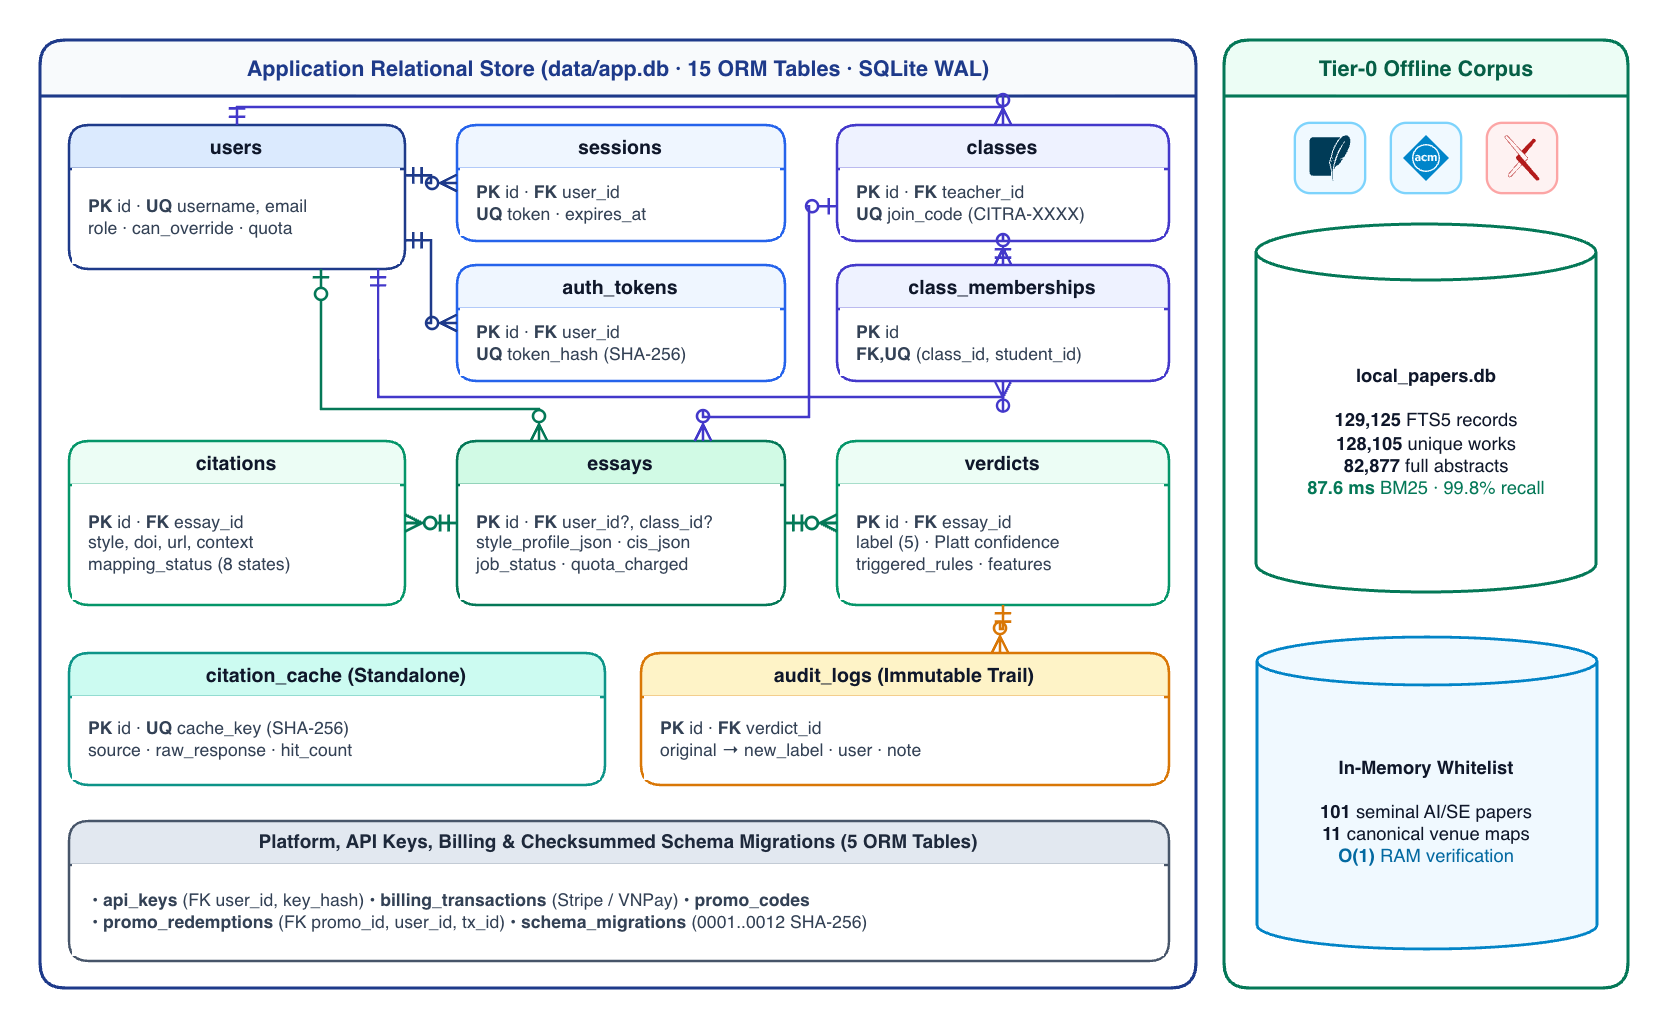
\includegraphics[width=\textwidth,keepaspectratio]{picture/figures/fig3_3_data_model.png}
    \caption[Crow's Foot Entity-Relationship Diagram of the 15-table database schema]{Crow's Foot Entity-Relationship Diagram (ERD) of the 15 application ORM tables (\texttt{app.db}) and the offline 129,125-record SQLite FTS5 scholarly corpus (\texttt{local\_papers.db}).}
    \label{fig:data-model}
\end{figure}

\subsection{Schema Migrations, SQLite WAL Tuning, and Audit Retention}

Schema evolution across versions is managed deterministically by \texttt{db/migrations.py}, which tracks thirteen numbered, SHA-256 checksummed migrations (\texttt{0001}--\texttt{0013}) inside \texttt{schema\_migrations} and verifies checksums at startup to detect accidental schema drift. For concurrent read/write throughput, \texttt{db/sqlite\_tuning.py} configures \texttt{PRAGMA journal\_mode=WAL}, \texttt{synchronous=NORMAL}, and \texttt{busy\_timeout=30000} on native POSIX disks while automatically detecting macOS VirtioFS or network bind mounts (where shared-memory \texttt{-shm} mmap files risk corruption) and switching safely to \texttt{DELETE} journal mode.

Regarding audit retention, \texttt{audit\_logs} exposes no HTTP update or individual delete endpoint during normal operation so that instructor overrides remain tamper-evident. When a user deletes an uploaded essay or executes self-service account deletion (\texttt{DELETE /api/users/me}), cascading cleanup removes child \texttt{citations}, \texttt{verdicts}, and associated \texttt{audit\_logs} rows within a single database transaction so referential integrity is preserved without orphaned records.

\section{API Contract, Deployment, and Security Design}

\subsection{REST and SSE API Surface}

All backend endpoints are mounted under the \texttt{/api} prefix in \texttt{api/\allowbreak main.py}~\cite{fastapi}, as detailed in Table~\ref{tab:api-surface}. Synchronous SQLite and filesystem operations run inside thread-pool executors so the main \texttt{asyncio} loop never blocks active SSE streams.

{\setlength{\tabcolsep}{3.5pt}
\begin{longtable}{|L{0.31}|L{0.69}|}
\caption{FastAPI REST and SSE endpoint groups mounted under \texttt{/api} (\texttt{v3.90.5}).}\label{tab:api-surface}\\
\hline
\textbf{Route Prefix} & \textbf{Principal Endpoints and Operations} \\
\hline
\endfirsthead
\multicolumn{2}{c}{\itshape Table \thetable\ (continued from previous page)}\\
\hline
\textbf{Route Prefix} & \textbf{Principal Endpoints and Operations} \\
\hline
\endhead
\hline
\multicolumn{2}{r}{\itshape Continued on next page}\\
\endfoot
\hline
\endlastfoot
\textbf{\texttt{/api/auth/*}} & \texttt{POST /register}, \texttt{/login}, \texttt{/google} \textbf{(OAuth2)}, \texttt{/logout}, \texttt{/activate}, \texttt{/forgot-password}, \texttt{/reset-password}, \texttt{GET /me}. \\
\hline
\textbf{\texttt{/api/essays/*}} & \texttt{POST /essays} (upload), \texttt{GET /essays}, \texttt{/essays/stats}, \texttt{/essays/\{id\}/status}, \texttt{/essays/\{id\}/events} \textbf{(SSE)}, \texttt{/essays/\{id\}/report} (\texttt{json|csv|pdf|docx}), \texttt{/essays/\{id\}/remediate}, \texttt{/essays/\{id\}/export-healed-docx}, \texttt{/essays/\{id\}/revision-diff}, \texttt{/essays/\{id\}/page-preview/\{p\}}, \texttt{POST /essays/\{id\}/share}, \texttt{GET /essays/shared/\{token\}}, \texttt{/essays/sandbox/*}. \\
\hline
\texttt{/api/essays/\allowbreak\{id\}/\allowbreak verdicts/*} & \texttt{POST /api/essays/\allowbreak\{id\}/\allowbreak verdicts/\allowbreak\{vid\}/override} (capability-gated teacher override + transactional CIS recalculation). \\
\hline
\textbf{\texttt{/api/teacher/*}} & \texttt{GET /dashboard}, \texttt{/classes}, \texttt{POST /classes/join}, \texttt{/classes/\{id\}/regenerate-code}, \texttt{GET /classes/\{id\}/analytics}, \texttt{/classes/\{id\}/pending-reviews}, \texttt{/classes/\{id\}/export.csv}, \texttt{/classes/\{id\}/export.zip}. \\
\hline
\textbf{\texttt{/api/users/*}} & Admin \texttt{/users} management; self-service \texttt{PATCH/DELETE /users/me}, \texttt{/users/me/password}, \texttt{/users/me/avatar}, and \texttt{/users/me/api-keys}. \\
\hline
\textbf{\texttt{/api/billing/*}} & \texttt{GET /plans}, \texttt{/subscription}, \texttt{POST /create-checkout-session}, Stripe \& VNPay \textbf{HMAC-SHA512} verification, \texttt{/cancel}, and admin \texttt{/admin/promos}. \\
\hline
\textbf{\texttt{/api/system/*}}, \textbf{\texttt{/api/audit/*}}, \textbf{\texttt{/api/cache}}, \textbf{\texttt{/api/export/*}} & \texttt{GET /api/health}, \texttt{GET /api/system/health}, \texttt{POST /api/system/circuit-breakers/reset}, \texttt{DELETE /api/cache}, \texttt{GET /api/audit/log}, \texttt{GET /api/export/report} (admin system summary). \\
\hline
\end{longtable}
}

\subsection{Container Deployment Topology and Defense-in-Depth Security}

Figure~\ref{fig:deployment} depicts the UML 2.5 Deployment Topology across development (\texttt{docker-compose.yml}) and hardened production (\texttt{docker-compose.prod.yml}). Three containers communicate over an isolated Docker bridge network: \texttt{essay-\allowbreak check-\allowbreak grobid} runs \texttt{grobid/grobid:0.9.1-crf} (chosen over heavier deep-learning images so structured PDF parsing runs deterministically within a 2--3\,GB JVM heap on CPU-only servers). Meanwhile, \texttt{integrity-api} runs Uvicorn/FastAPI, and \texttt{integrity-web} serves the compiled SPA via Nginx 1.27 with TLS 1.2/1.3, Content-Security-Policy, HTTP Strict-Transport-Security, and unbuffered SSE proxying (\texttt{X-Accel-Buffering: no}). In production, ports \texttt{8000} and \texttt{8070} bind strictly to internal/loopback interfaces rather than the public Internet.

\begin{figure}[H]
    \centering
    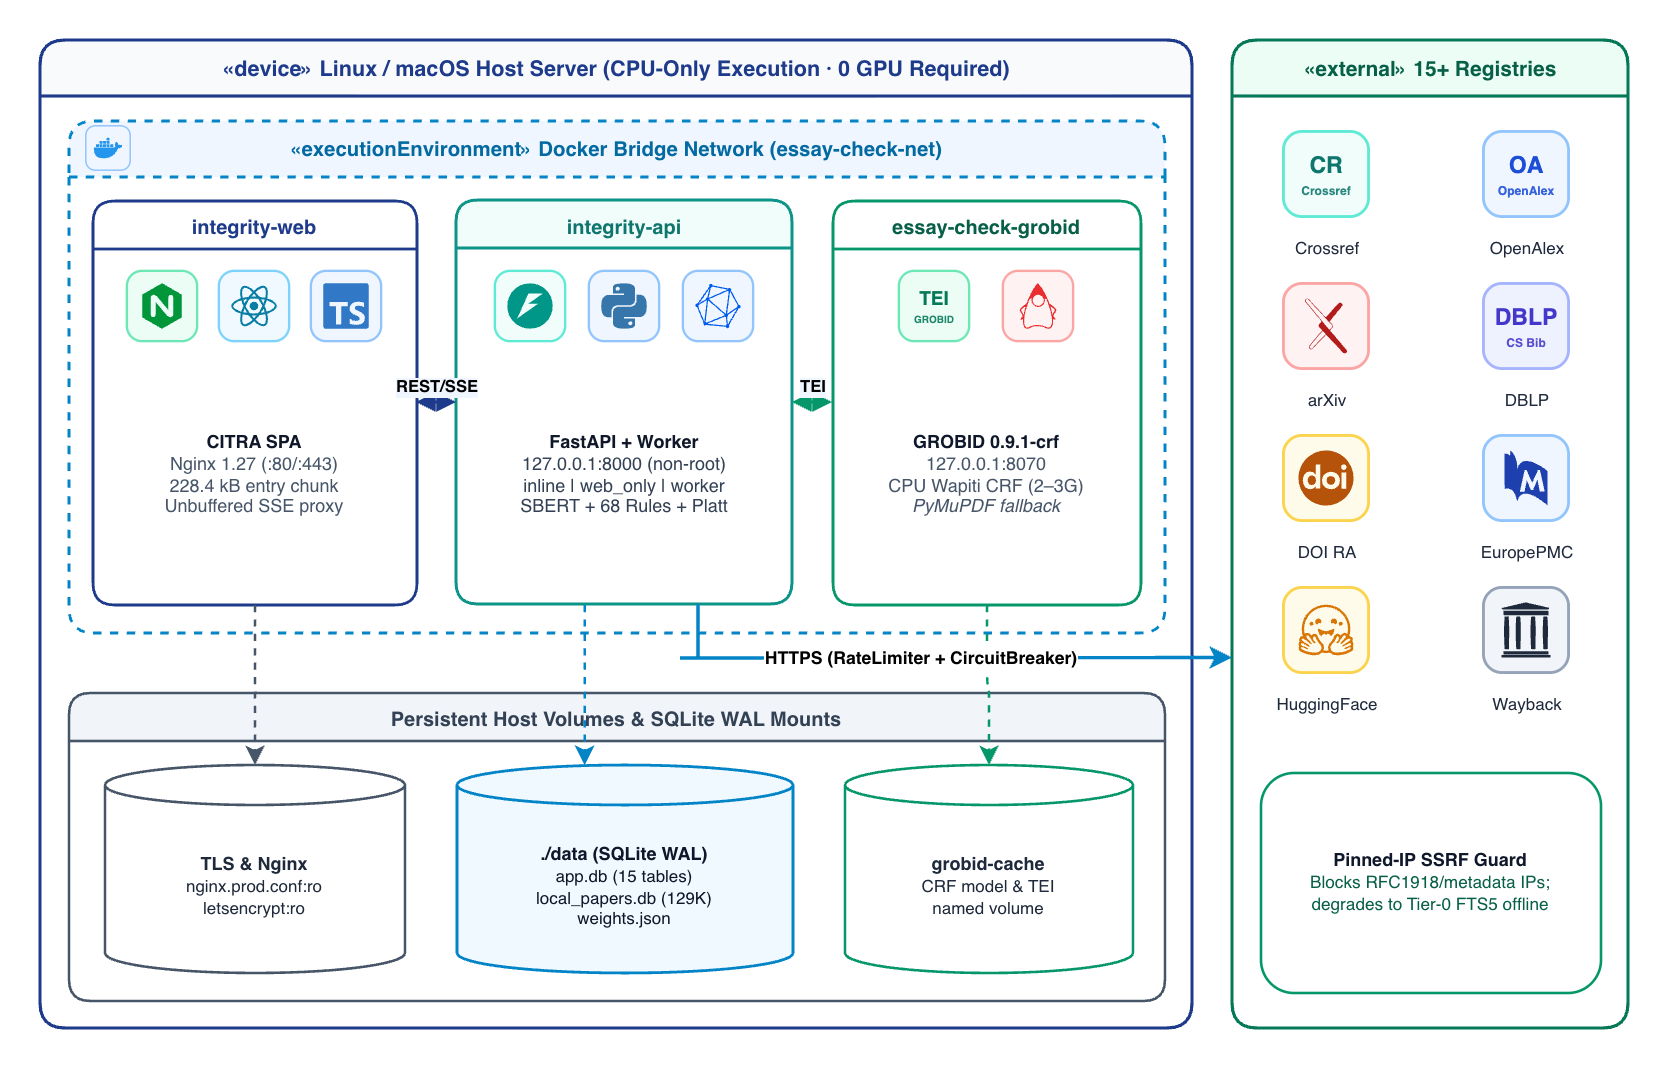
\includegraphics[width=\textwidth,keepaspectratio]{picture/figures/fig3_4_deployment.png}
    \caption[UML 2.5 Deployment diagram of the three-container CITRA platform]{UML 2.5 Deployment topology coordinating Nginx (\texttt{integrity-web}), FastAPI (\texttt{integrity-api}), and CPU-tuned \texttt{grobid:0.9.1-crf} with persistent SQLite volumes.}
    \label{fig:deployment}
\end{figure}

Defense-in-depth security controls span four boundaries:
\begin{itemize}
    \item \textbf{Token and Credential Hardening:} Passwords use salted \texttt{bcrypt} hashes; one-time email tokens (\texttt{auth\_tokens.token\_hash}) and personal API keys (\texttt{api\_keys.key\_hash}) store only SHA-256 digests in SQLite, while public share receipts use stateless HMAC-SHA256 signatures. Production startup aborts if \texttt{JWT\_SECRET} remains at its development placeholder.
    \item \textbf{Pinned-IP SSRF Defense:} The \texttt{LinkValidator} and \texttt{SafeHtml\allowbreak Meta\allowbreak Verifier} modules resolve hostnames prior to connection, block loopback, link-local, RFC 1918 private, and cloud-metadata IP ranges (\texttt{169.254.\allowbreak 169.254}), re-validate every HTTP redirect hop, and connect via a custom \texttt{httpx} transport pinned to the verified IP address to defeat DNS rebinding.
    \item \textbf{Upload and Export Sanitization:} Uploads check PDF (\texttt{\%PDF-}) and ZIP/DOCX (\texttt{PK\textbackslash x03\textbackslash x04}) magic bytes, enforce strict byte/page caps, and neutralize spreadsheet formula prefixes (\texttt{=}, \texttt{+}, \texttt{-}, \texttt{@}) in CSV exports.
    \item \textbf{Anti-IDOR Ownership and Rate-Limiting Guards:} Every essay, verdict, share-token, and classroom endpoint enforces explicit resource-ownership checks (\texttt{user\_id} or supervised \texttt{class\_id}) before returning data, while authentication and upload endpoints enforce token-bucket rate limits and atomic Compare-And-Swap (\texttt{CAS}) quota accounting.
\end{itemize}

\section{Chapter Summary}

This chapter specified sixteen atomic functional requirements (IEEE 29148), ten quantitative non-functional requirements (ISO/IEC 25010), UML 2.5 use case and sequence models, the 15-table SQLAlchemy schema with thirteen SHA-256 checksummed migrations (\texttt{0001}--\texttt{0013}), the \texttt{/api/*} REST/SSE contract, and the security-hardened Docker deployment. Chapter~\ref{chap:architecture} details the internal software architecture and algorithms across all eight pipeline layers.


\newpage
\chapter{System Architecture and Implementation}
\label{chap:architecture}

\section{Architectural Overview}

\subsection{Eight-Layer Pipeline and Graceful Degradation}

\textbf{CITRA} organizes manuscript verification into an acyclic sequence of eight software layers, summarized in Table~\ref{tab:layers} and illustrated in Figure~\ref{fig:architecture}. Each layer accepts typed data structures and emits explicit status metadata so individual stages can be unit-tested or replaced independently.

{\setlength{\tabcolsep}{3.5pt}
\begin{longtable}{|L{0.18}|L{0.34}|L{0.48}|}
\caption{Responsibilities and core Python/TypeScript modules of the eight system layers.}\label{tab:layers}\\
\hline
\textbf{Layer} & \textbf{Principal Modules} & \textbf{Core Responsibility} \\
\hline
\endfirsthead
\multicolumn{3}{c}{\itshape Table \thetable\ (continued from previous page)}\\
\hline
\textbf{Layer} & \textbf{Principal Modules} & \textbf{Core Responsibility} \\
\hline
\endhead
\hline
\multicolumn{3}{r}{\itshape Continued on next page}\\
\endfoot
\hline
\endlastfoot
\textbf{1. Extraction} & \texttt{document\_parser}, \texttt{grobid\_parser}, \texttt{grobid\_adapter}, \texttt{docx\_parser}, \texttt{patterns/*}, \texttt{style\_detector} & Parse PDF, DOCX, BibTeX, and RIS inputs into body text, contextual in-text markers, and bibliography entries across \textbf{12 styles}. \\
\hline
\textbf{2. Merging} & \texttt{integrity\_pipeline.\_merge\_citations} & Deduplicate in-text, bibliography, and appendix citations into unique referenced works while keeping all inline occurrences. \\
\hline
\textbf{3. Linking} & \texttt{citation\_linker}, \texttt{duplicate\_detector}, \texttt{statuses} & Reconstruct the bipartite graph between inline markers and bibliography entries across \textbf{7 resolution methods} and \textbf{8 statuses}. \\
\hline
\textbf{4. Retrieval} & \texttt{retrieval\_orchestrator}, \texttt{local\_db}, \texttt{link\_validator}, \texttt{html\_meta\_verifier}, 15+ clients & Route queries across offline SQLite FTS5, \textbf{15+ live APIs}, Retraction Watch, and SSRF-safe HTTP/Wayback/HTML checks. \\
\hline
\textbf{5. Matching} & \texttt{features}, \texttt{fuzzy}, \texttt{semantic}, \texttt{author\_matcher}, \texttt{venue\_normalizer} & Compute lexical similarity, metadata distances, SBERT sentence-pooled alignment, stance, and ONNX INT8 \texttt{VI}$\leftrightarrow$\texttt{EN} scores. \\
\hline
\textbf{6. Verification} & \texttt{neuro\_symbolic\_checker}, \texttt{rules}, \texttt{vn\_legal\_verifier}, \texttt{calibration} & Evaluate Order 0 + 16 symbolic rule groups (\textbf{68 rule IDs}) blended with 16D Logistic Regression and Platt calibration. \\
\hline
\textbf{7. Scoring \& Export} & \texttt{cis}, \texttt{explanation}, \texttt{bibliography\_formatter}, \texttt{docx\_exporter} & Compute the \textbf{five-component CIS}, render bilingual explanations, and export sanitized reports and repaired \texttt{.docx} files. \\
\hline
\textbf{8. Presentation} & FastAPI \texttt{api/*}, React/TypeScript \texttt{web/src/*} & Serve SSE progress, six diagnostic report views, classroom analytics, inline teacher overrides, and admin health controls. \\
\hline
\end{longtable}
}

\begin{figure}[H]
    \centering
    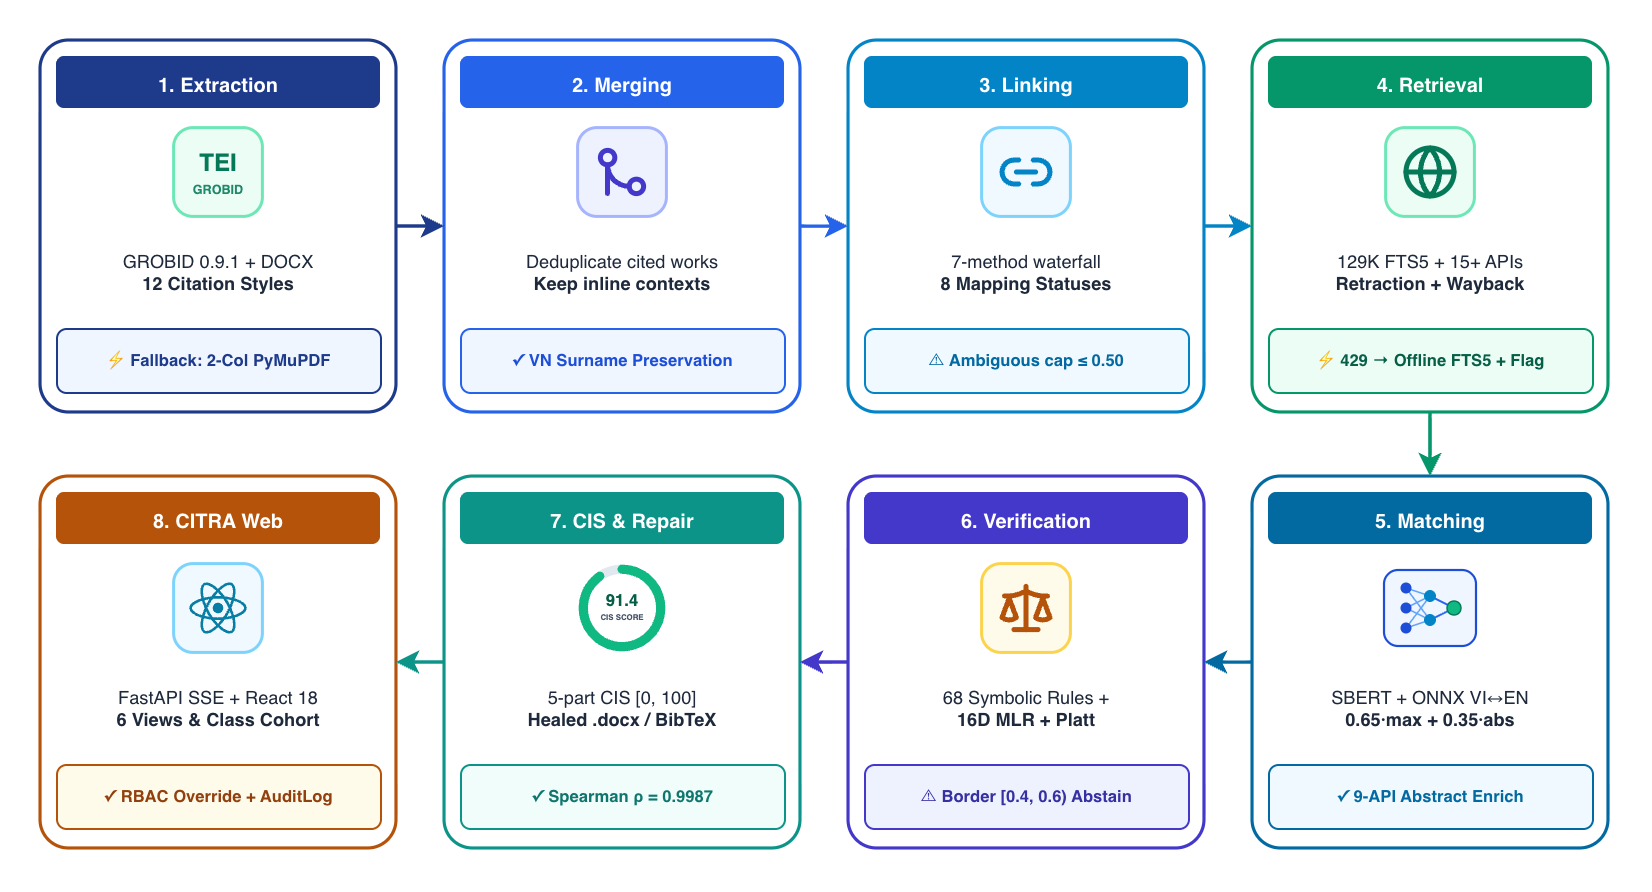
\includegraphics[width=\textwidth,keepaspectratio]{picture/figures/fig4_1_architecture.png}
    \caption[Eight-layer software architecture and graceful degradation contracts]{Eight-layer software architecture of CITRA (\texttt{v3.90.9}) showing inter-layer contracts and graceful degradation fallbacks.}
    \label{fig:architecture}
\end{figure}

Every layer enforces a strict \emph{graceful degradation contract}. If the GROBID container is unreachable, Layer 1 falls back automatically to two-column PyMuPDF and regex parsing. Similarly, if live registries return HTTP 429 or time out, Layer 4 falls back to the 129,137-record offline FTS5 index and records \texttt{api\_exhausted = True}, while Layer 6 emits \texttt{unresolved} rather than guessing whenever evidence remains incomplete.

\subsection{Software Design Patterns}

Five classical object-oriented and cloud resilience patterns keep the codebase modular and maintainable:
\begin{itemize}
    \item \textbf{Strategy and Priority Registry (\texttt{extraction/patterns/}):} Twelve citation-style parsers inherit from the \texttt{CitationFormat} base class and register integer priorities so style-specific rules remain isolated from the document reader.
    \item \textbf{Adapter (\texttt{grobid\_adapter.py} \& API Clients):} Heterogeneous external formats (GROBID TEI-XML, Crossref JATS XML, OpenAlex inverted abstract indices, arXiv Atom XML, and BibTeX) are normalized into uniform internal \texttt{Citation} and \texttt{ScholarlyCandidate} objects.
    \item \textbf{Chain of Responsibility (\texttt{CitationLinker} \& \texttt{SymbolicRules}):} Both the seven-method linker and the 16-group symbolic verifier evaluate ordered handlers and short-circuit as soon as a decisive condition fires.
    \item \textbf{Circuit Breaker and Token-Bucket Rate Limiter (\texttt{retrieval/}):} Each external API client is wrapped in a state machine (\texttt{closed} $\rightarrow$ \texttt{open} $\rightarrow$ \texttt{half\_open}) and a thread-safe rate limiter so a slow or failing upstream provider is temporarily bypassed without stalling concurrent essays.
    \item \textbf{Singleflight Request Coalescing:} Identical normalized queries arriving concurrently across batch uploads share a single in-flight HTTP coroutine before persisting the result in \texttt{citation\_cache}.
\end{itemize}

\section{Extraction Layer}

\subsection{Multi-Format Document Parsing}

Manuscript ingestion (\texttt{DocumentParser}) handles four input formats: PDF, DOCX, BibTeX, and RIS. For PDF files, the primary \texttt{grobid\_hybrid} path submits the binary stream to GROBID \texttt{0.9.1-crf}~\cite{Lopez2009}, extracting body paragraphs, inline \texttt{<ref type="bibr">} pointers, sentence windows, and \texttt{<biblStruct>} entries. Two post-processors correct recurring student-report artifacts in GROBID output: (1) a \emph{table-of-contents (TOC) and dot-leader filter} discards numbered chapter headings that mimic numbered references, and (2) a \emph{regex field-enrichment pass} recovers URLs, publishers, Vietnamese statutory codes, and humanities page ranges omitted from TEI-XML tags.

When GROBID is disabled or encounters non-standard word-processor layouts, \texttt{DocumentParser} falls back to a two-column geometry-aware PyMuPDF~\cite{PyMuPDF2024} and \texttt{pdfplumber}~\cite{Pdfplumber2024} pipeline. Pages with near-zero extractable character density trigger selective Tesseract Vietnamese/English OCR, whereas legacy Vietnamese encodings (VNI and TCVN3) are normalized to NFC Unicode. Native \texttt{.docx} manuscripts are parsed directly via \texttt{python-docx} paragraph styles and XML numbering properties without intermediate PDF conversion loss.

\subsection{Twelve Citation Style Modules and Style Detection}

Bibliography entries and inline markers are matched against twelve modular conventions listed in priority order in Table~\ref{tab:styles} and depicted in Figure~\ref{fig:extraction}. Integer priorities resolve syntactic overlaps (such as bracketed ordinals shared by IEEE, ACM, and Vancouver). In parallel, \texttt{StyleDetector} scores document-wide structural ratios to output a \texttt{StyleProfile} (\texttt{APA-like}, \texttt{IEEE-like}, \texttt{MIXED}, or \texttt{UNKNOWN}); documents mixing incompatible conventions above $30\%$ receive a style-inconsistency flag.

{\setlength{\tabcolsep}{3.5pt}
\begin{longtable}{|L{0.16}|C{0.12}|L{0.33}|L{0.39}|}
\caption{Twelve registered citation style extractors and their structural patterns.}\label{tab:styles}\\
\hline
\textbf{Style} & \textbf{Priority} & \textbf{In-Text Marker Pattern} & \textbf{Bibliography Entry Pattern} \\
\hline
\endfirsthead
\multicolumn{4}{c}{\itshape Table \thetable\ (continued from previous page)}\\
\hline
\textbf{Style} & \textbf{Priority} & \textbf{In-Text Marker Pattern} & \textbf{Bibliography Entry Pattern} \\
\hline
\endhead
\hline
\multicolumn{4}{r}{\itshape Continued on next page}\\
\endfoot
\hline
\endlastfoot
\textbf{APA (7th)} & \textbf{100} & \textit{(Author et al., 2020)}, \textit{Author (2020a)} & Author, A. B. (2020). Title of work. \textit{Venue, 12}(3), 45--67. \\
\hline
\textbf{IEEE} & \textbf{90} & \textit{[1]}, \textit{[1, 2]}, \textit{[1]--[3]} & [1] A. Author, ``Title,'' \textit{Venue}, vol.\ 1, pp.\ 1--10, 2020. \\
\hline
\textbf{ACM} & 88 & \textit{[1]}, \textit{[Author 2020]} & [1] Author Name. 2020. Title. In \textit{Proc.\ ACM}, 1--10. \\
\hline
\textbf{Harvard} & 85 & \textit{(Author, 2020)}, \textit{(Author 2020: 15)} & Author, A. (2020) \textit{Title}. Place: Publisher. \\
\hline
\textbf{Vancouver} & 80 & \textit{[1]}, \textit{(1--3)} & 1. Author AB. Title. \textit{Venue}. 2020;12(1):10--20. \\
\hline
\textbf{Nature} & 78 & Superscript / \textit{[1]} & 1. Author, A. Title. \textit{Nature} \textbf{580}, 100--105 (2020). \\
\hline
\textbf{CSE} & 77 & \textit{(Author 2020)}, superscript & Author AB. 2020. Title. \textit{Venue}. 12(1):10--20. \\
\hline
\textbf{ACS} & 76 & \textit{(1)}, superscript & (1) Author, A. B. Title. \textit{J.\ Am.\ Chem.\ Soc.} \textbf{2020}, \textit{142}, 1--5. \\
\hline
\textbf{AMA} & 75 & Superscript / \textit{[1]} & 1. Author AB. Title. \textit{JAMA}. 2020;323(1):1--10. \\
\hline
\textbf{Chicago} & 70 & \textit{(Author 2020, 45)}, footnote & Author, First. 2020. \textit{Title}. Place: Publisher. \\
\hline
\textbf{MLA (9th)} & 70 & \textit{(Author 45)}, \textit{(Author and Coauthor 12)} & Author, First. ``Title.'' \textit{Venue}, vol.\ 1, no.\ 2, 2020, pp.\ 1--15. \\
\hline
\textbf{VN Legal} & \textbf{Rule} & \begin{vietnamese}\textit{(Luật số 20/2023/QH15)}\end{vietnamese} & \begin{vietnamese}Quốc hội / Chính phủ. (2023). \textit{Luật / Nghị định / Thông tư}.\end{vietnamese} \\
\hline
\end{longtable}
}

\begin{figure}[H]
    \centering
    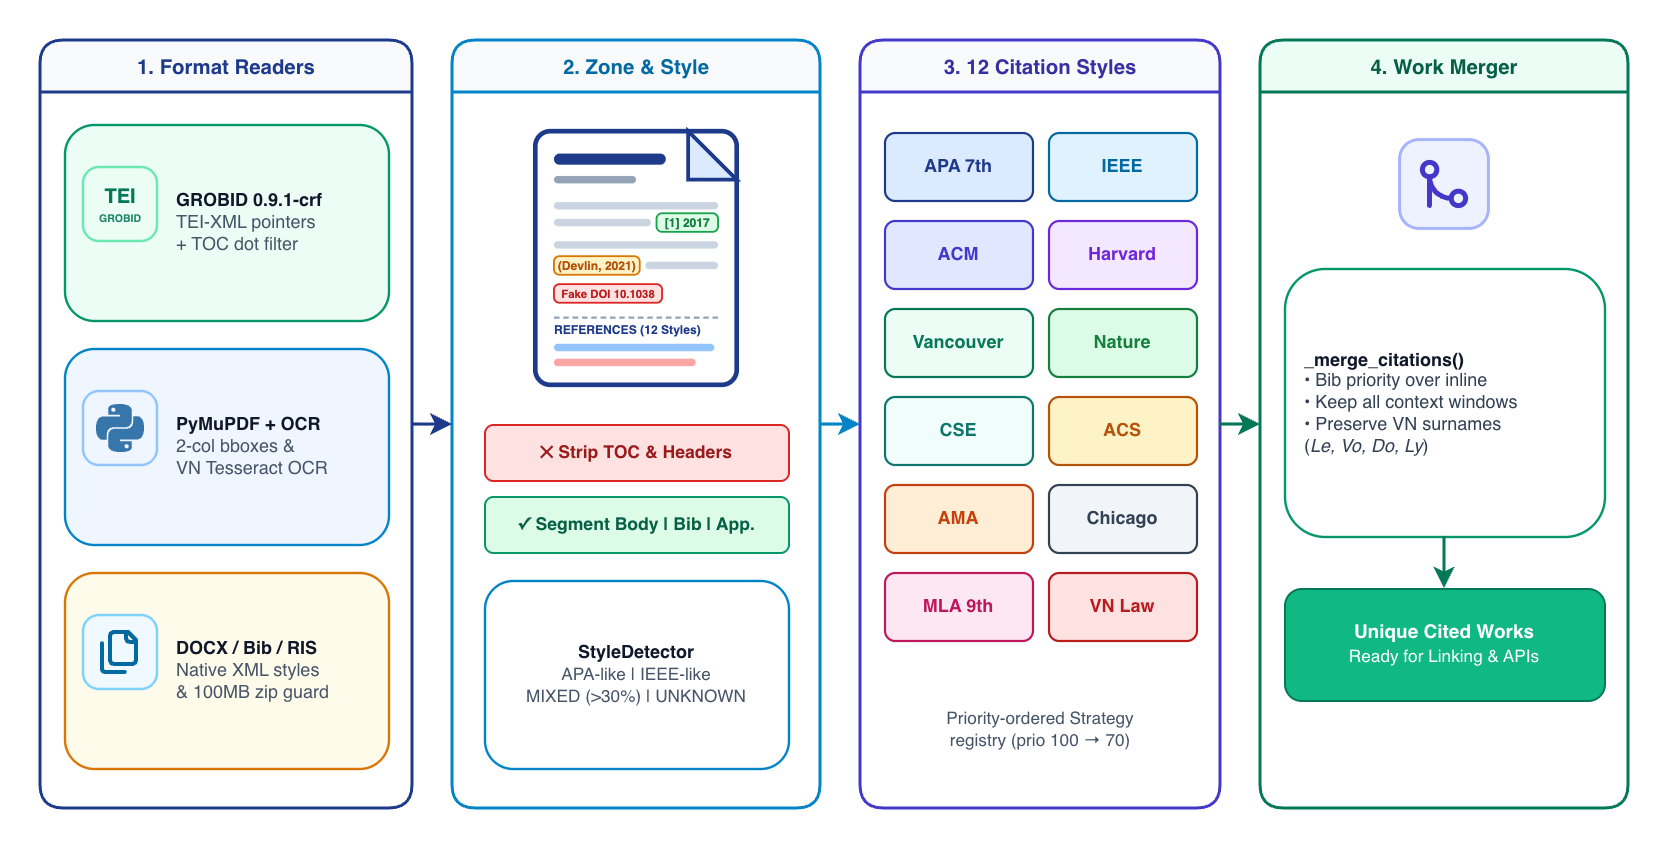
\includegraphics[width=\textwidth,keepaspectratio]{picture/figures/fig4_2_extraction.png}
    \caption[Multi-format extraction pipeline across PDF, DOCX, BibTeX, and RIS]{Extraction layer architecture combining GROBID \texttt{0.9.1-crf} TEI-XML, TOC filtering, two-column PyMuPDF fallback, selective OCR, and twelve style parsers.}
    \label{fig:extraction}
\end{figure}

\section{Merging and Bidirectional Linking}

\subsection{Work-Level Citation Merging}

Extraction yields three raw lists: body in-text markers, bibliography entries, and appendix citations. \texttt{IntegrityPipeline.\_merge\_citations} fuses matching markers and bibliography entries into a deduplicated set of unique referenced works while keeping every inline occurrence attached as a contextual observation. Short Vietnamese family names (such as \textit{Le}, \textit{Vo}, \textit{Do}, \textit{Ho}, and \textit{Ly}) are explicitly preserved during surname normalization so two-letter Vietnamese surnames are never stripped as initials. Compound markers such as \texttt{[9, 10]} or \texttt{(Vaswani et al., 2017; Devlin et al., 2019)} are expanded into individual edges, and composite numbered entries (\texttt{[14] a) ... b) ...}) are split into sub-indexed items (\texttt{14a}, \texttt{14b}).

\subsection{Seven-Method Linker and Eight Mapping Statuses}

Internal structural integrity requires a coherent bipartite graph between inline claims and the reference list. As shown in Figure~\ref{fig:linking}, \texttt{CitationLinker} runs a seven-stage resolution waterfall (plus instructor override) ordered by reliability in Table~\ref{tab:mapping-methods}, and assigns one of eight \texttt{MappingStatus} labels in Table~\ref{tab:mapping-statuses}. Duplicate bibliography entries are detected via exact DOI/arXiv match or $\ge 0.92$ combined title--author--year similarity. When \texttt{ambiguous\_mapping} occurs (for example, two papers by the same first author in the same year lacking \texttt{2024a}/\texttt{2024b} suffixes), downstream verification caps confidence at $0.50$ and forces \texttt{unresolved}.

\begin{figure}[H]
    \centering
    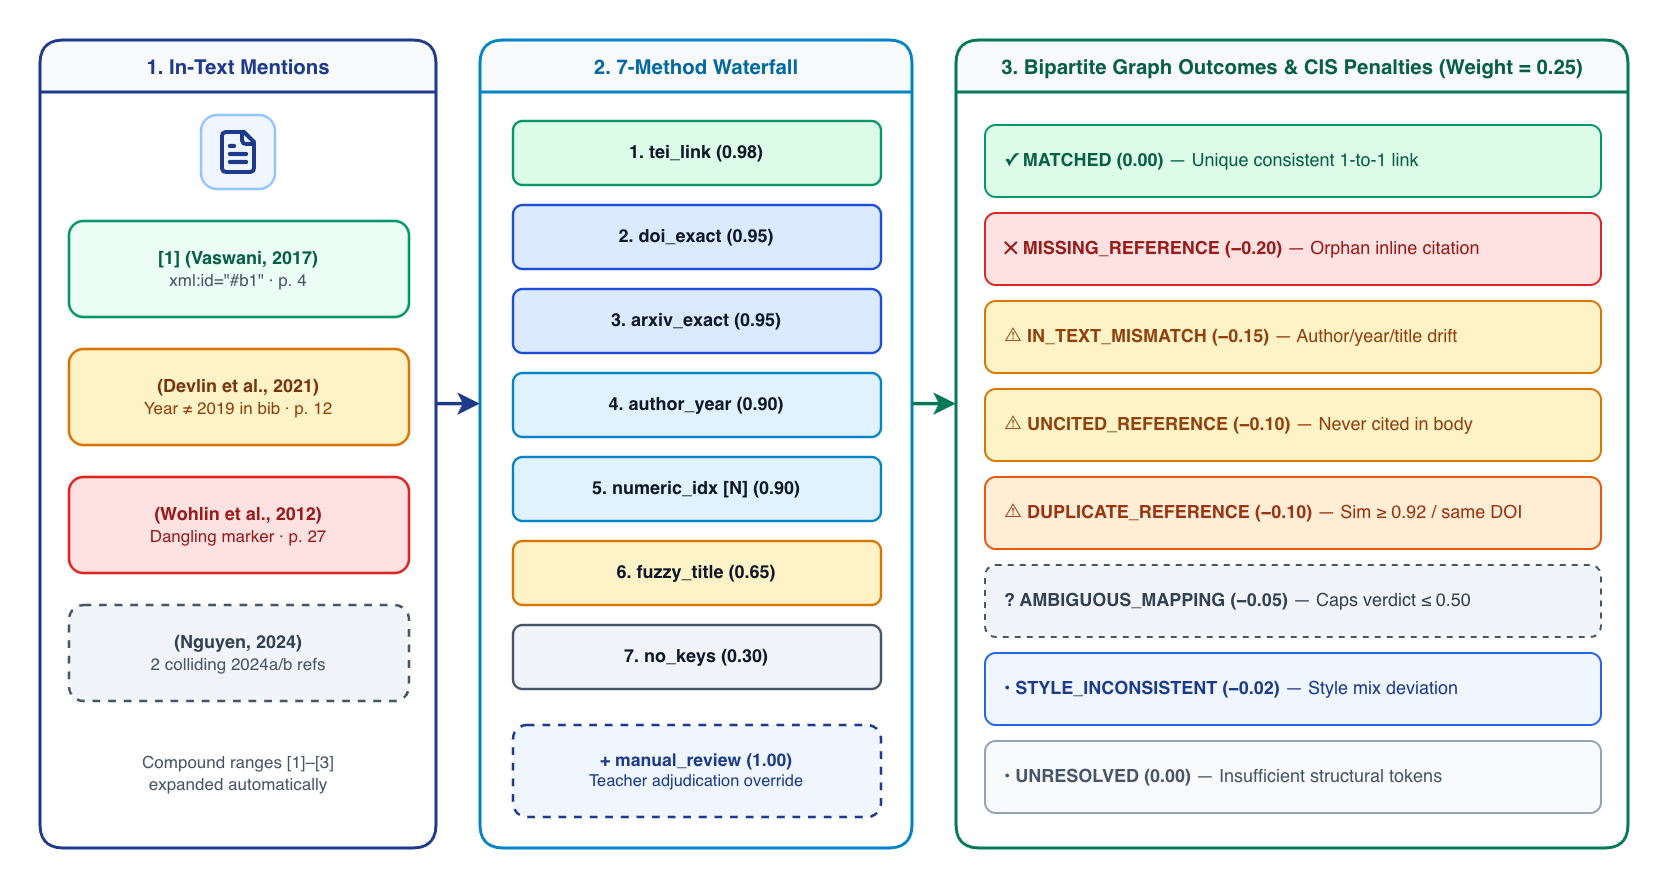
\includegraphics[width=\textwidth,keepaspectratio]{picture/figures/fig4_3_linking.png}
    \caption[Seven-method bidirectional citation linking waterfall and eight mapping statuses]{Bidirectional citation linking waterfall across seven automated resolution methods and the resulting eight structural mapping statuses.}
    \label{fig:linking}
\end{figure}

{\setlength{\tabcolsep}{3.5pt}
\begin{longtable}{|L{0.25}|C{0.15}|L{0.60}|}
\caption{Ordered resolution methods in \texttt{CitationLinker}.}\label{tab:mapping-methods}\\
\hline
\textbf{Method} & \textbf{Default Conf.} & \textbf{Matching Criterion} \\
\hline
\endfirsthead
\multicolumn{3}{c}{\itshape Table \thetable\ (continued from previous page)}\\
\hline
\textbf{Method} & \textbf{Default Conf.} & \textbf{Matching Criterion} \\
\hline
\endhead
\hline
\multicolumn{3}{r}{\itshape Continued on next page}\\
\endfoot
\hline
\endlastfoot
\textbf{\texttt{tei\_link}} & \textbf{0.98} & Direct GROBID TEI-XML \texttt{xml:id} pointer from inline \texttt{<ref>} to \texttt{<biblStruct>}. \\
\hline
\textbf{\texttt{doi\_exact}} & \textbf{0.95} & Identical normalized DOI present in both inline marker and reference entry. \\
\hline
\textbf{\texttt{arxiv\_exact}} & \textbf{0.95} & Identical canonical \texttt{arXiv} identifier present on both sides. \\
\hline
\textbf{\texttt{author\_year}} & 0.90 & Normalized surname(s), year, and optional suffix (\texttt{a}--\texttt{f}) agree (including MLA author--page inference). \\
\hline
\textbf{\texttt{numeric\_index}} & 0.90 & Bracketed or superscript ordinal (or expanded range \texttt{[1]--[3]}) matches bibliography index. \\
\hline
\textbf{\texttt{fuzzy}} & 0.65 & Partial title or author token overlap above fallback threshold when exact keys are missing. \\
\hline
\textbf{\texttt{no\_keys}} & 0.30 & Insufficient disambiguating keys or tie across multiple entries (\texttt{ambiguous\_mapping}). \\
\hline
\textbf{\texttt{manual\_review}} & \textbf{1.00} & Link explicitly adjudicated by an authorized instructor. \\
\hline
\end{longtable}
}

{\setlength{\tabcolsep}{3.5pt}
\begin{longtable}{|L{0.28}|C{0.15}|C{0.14}|L{0.43}|}
\caption{Eight structural mapping statuses and their CIS rubric penalties.}\label{tab:mapping-statuses}\\
\hline
\textbf{Mapping Status} & \textbf{Integrity Issue} & \textbf{CIS Penalty} & \textbf{Structural Meaning} \\
\hline
\endfirsthead
\multicolumn{4}{c}{\itshape Table \thetable\ (continued from previous page)}\\
\hline
\textbf{Mapping Status} & \textbf{Integrity Issue} & \textbf{CIS Penalty} & \textbf{Structural Meaning} \\
\hline
\endhead
\hline
\multicolumn{4}{r}{\itshape Continued on next page}\\
\endfoot
\hline
\endlastfoot
\textbf{\texttt{matched}} & No & 0.00 & Unique one-to-one link with consistent author/year metadata. \\
\hline
\textbf{\texttt{missing\_reference}} & \textbf{Yes} & \textbf{0.20} & Inline marker cites a source absent from the bibliography (orphan citation). \\
\hline
\textbf{\texttt{in\_text\_mismatch}} & \textbf{Yes} & \textbf{0.15} & Linked pair disagrees on publication year, surname, or title tokens. \\
\hline
\textbf{\texttt{uncited\_reference}} & \textbf{Yes} & \textbf{0.10} & Bibliography entry is never cited anywhere in the manuscript body. \\
\hline
\textbf{\texttt{duplicate\_reference}} & \textbf{Yes} & \textbf{0.10} & Two or more bibliography entries refer to the same publication. \\
\hline
\textbf{\texttt{ambiguous\_mapping}} & \textbf{Yes} & 0.05 & Inline marker collides equally with multiple bibliography entries. \\
\hline
\textbf{\texttt{style\_inconsistent}} & \textbf{Yes} & 0.02 & Entry or marker deviates from the manuscript's dominant style profile. \\
\hline
\textbf{\texttt{unresolved}} & No & 0.00 & Insufficient structural tokens to classify link state. \\
\hline
\end{longtable}
}

\section{Federated Retrieval and URL Verification}

\subsection{Domain-Aware Multi-Tier Orchestration}

Rather than broadcasting every reference to every external API, \texttt{Retrieval\allowbreak Orchestrator} routes queries through the tiered architecture shown in Figure~\ref{fig:retrieval}:
\begin{enumerate}
    \item \textbf{Pre-Screening:} Pure web URLs, software repositories, IETF RFCs, PyPI packages, Hugging Face cards, and Vietnamese legal documents (\texttt{parse\_vn\_legal\_reference} + \texttt{VNLegalVerifier}) are routed directly to specialized technical/legal verifiers.
    \item \textbf{Tier 0 (Offline Sub-100\,ms Lookup):} Queries first check the 101-paper seminal whitelist (\texttt{\_KNOWN\_PAPERS}) and the local SQLite FTS5 database (\texttt{local\_papers.db}, 129,137 records covering 128,115 unique papers and 82,887 full abstracts) using Okapi BM25 across exact-title, year-constrained, and author-constrained queries.
    \item \textbf{Tier 1 (Domain-Routed Public APIs):} Using identifier cues (DOI, arXiv ID, ISBN, PMID) and lexical domain regexes (CS/AI, Biomedicine, Books, Repositories), async queries dispatch under configured token-bucket rate limits (\texttt{configs/config.yaml}). Specifically, \textbf{Crossref} ($25\text{\,req/s}$ polite pool + Retraction Watch flags), \textbf{OpenAlex} ($8\text{\,req/s}$), \textbf{DataCite}, \textbf{Global DOI RA}, \textbf{DOAJ}, and \textbf{OpenAIRE/HAL} cover general and open-access venues, while \textbf{DBLP} ($1.5\text{\,req/s}$), \textbf{arXiv} ($1.0\text{\,req/s}$), \textbf{Europe PMC} ($5.0\text{\,req/s}$), \textbf{NCBI/bioRxiv}, \textbf{OpenLibrary / Google Books} ($3.0\text{\,req/s}$), and \textbf{Wikidata / OpenCitations} cover domain-specific records.
    \item \textbf{Tier 2 (Fallback \& Abstract Recovery):} Zero-hit queries optionally consult the \textbf{Serper / SerpAPI} router, and any winning candidate lacking an abstract triggers a 9-source \texttt{\_enrich\_missing\_abstract} pass so semantic claim alignment retains abstract coverage.
\end{enumerate}

\begin{figure}[H]
    \centering
    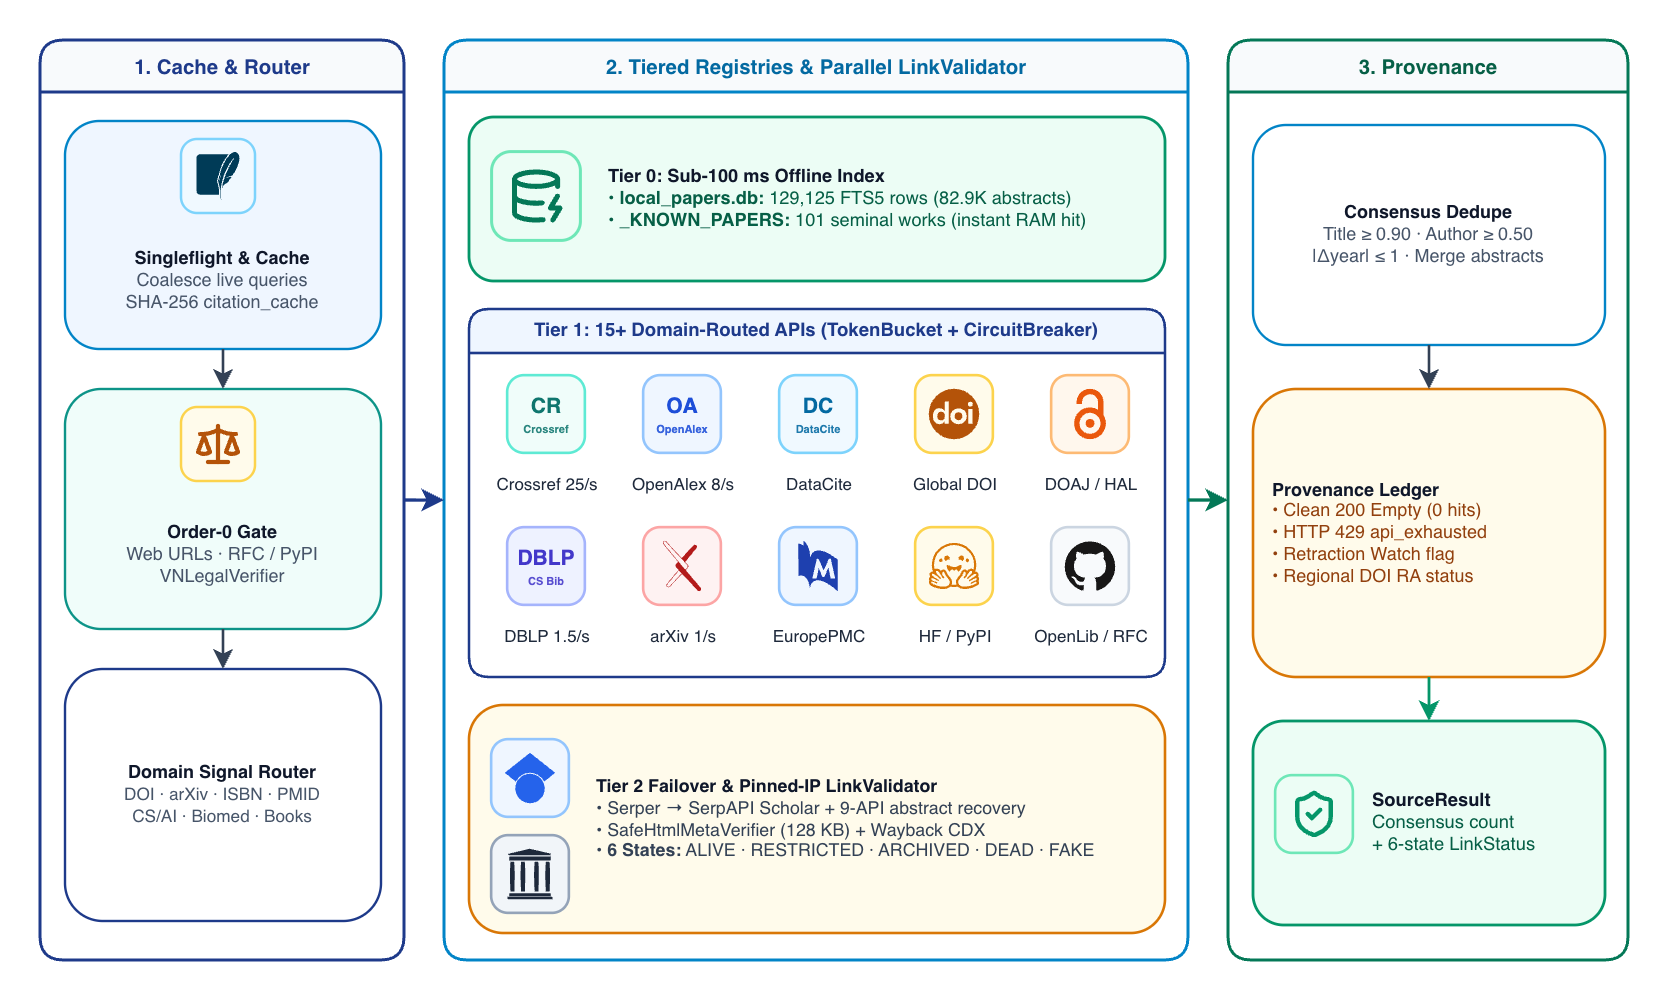
\includegraphics[width=\textwidth,keepaspectratio]{picture/figures/fig4_4_retrieval.png}
    \caption[Domain-aware multi-tier retrieval and SSRF-safe URL validation]{Domain-aware retrieval orchestration across Tier 0 (SQLite FTS5 + 101 known papers), Tier 1 (15+ live APIs), Tier 2 fallback, and parallel HTTP/Wayback/HTML verification.}
    \label{fig:retrieval}
\end{figure}

\subsection{Consensus, LinkValidator, and SafeHtmlMetaVerifier}
\label{sec:consensus}

Returned candidates are deduplicated and scored for multi-source consensus (\texttt{title\_sim} $\ge 0.90$, \texttt{author\_jaccard} $\ge 0.50$, $|\Delta y| \le 1$), inheriting abstracts across agreeing registries when one record omits abstract text. Simultaneously, \texttt{LinkValidator} probes cited URLs via pinned-IP SSRF-safe \texttt{HEAD}/\texttt{GET} requests and Internet Archive Wayback CDX lookups, assigning one of \textbf{six \texttt{LinkStatus} states}: \texttt{alive} (HTTP 200--399), \texttt{restricted\_alive} (HTTP 401/403/405/429 publisher anti-bot/paywall), \texttt{archived\_alive} (dead live link recovered in Wayback Machine), \texttt{dead\_link} (HTTP 404/410 or DNS NXDOMAIN), \texttt{fake\_domain} (RFC 2606 reserved/placeholder domains), or \texttt{unchecked}. For reachable web resources, \texttt{SafeHtmlMetaVerifier} streams up to $128\text{\,KB}$ of HTML (\texttt{MAX\_HTML\_HEAD\_BYTES = 131,072}) to extract Highwire Press (\texttt{citation\_title}, \texttt{citation\_author}, \texttt{citation\_doi}), Dublin Core, OpenGraph, and JSON-LD metadata while detecting bilingual English/Vietnamese ``Soft-404'' error pages disguised under HTTP 200 responses.

\section{Lexical, Neural, and Cross-Lingual Matching}

\subsection{Lexical and Bibliographic Field Matching}

Given the top candidate from retrieval, \texttt{FeatureCalculator} computes the structured \texttt{MatchFeatures} signals summarized in Table~\ref{tab:features}. Three domain normalizers prevent false metadata errors on legitimate scholarship. First, colon-delimited subtitle and edition stripping (\textit{2nd ed.}, \textit{Revised edition}) grants $0.95$ title similarity to clean main-title prefixes. Second, arXiv-to-proceedings year reconciliation computes \texttt{year\_distance} as the minimum $|\Delta y|$ across matching preprint and published versions of the same work, while \texttt{VenueNormalizer} expands conference and journal aliases (such as \texttt{NeurIPS} $\leftrightarrow$ \texttt{Advances in Neural Information Processing Systems}).

{\setlength{\tabcolsep}{3.5pt}
\begin{longtable}{|L{0.28}|C{0.12}|L{0.60}|}
\caption{Primary matching features computed by \texttt{FeatureCalculator} and \texttt{LinkValidator}.}\label{tab:features}\\
\hline
\textbf{Feature Name} & \textbf{Type} & \textbf{Computation} \\
\hline
\endfirsthead
\multicolumn{3}{c}{\itshape Table \thetable\ (continued from previous page)}\\
\hline
\textbf{Feature Name} & \textbf{Type} & \textbf{Computation} \\
\hline
\endhead
\hline
\multicolumn{3}{r}{\itshape Continued on next page}\\
\endfoot
\hline
\endlastfoot
\textbf{\texttt{title\_sim\_fuzzy}} & \texttt{float} & Max of normalized exact match, subtitle-prefix match ($0.95$), guarded substring ($0.90$), and RapidFuzz \texttt{token\_set\_ratio}. \\
\hline
\textbf{\texttt{title\_sim\_semantic}} & \texttt{float} & Cosine similarity between \texttt{all-MiniLM-L6-v2} embeddings of cited and candidate titles. \\
\hline
\textbf{\texttt{title\_sim\_max}} & \texttt{float} & Maximum of \texttt{title\_sim\_fuzzy} and \texttt{title\_sim\_semantic}. \\
\hline
\textbf{\texttt{author\_jaccard}} & \texttt{float} & Diacritic-folded surname overlap preserving short Vietnamese surnames (\textit{Le}, \textit{Vo}, \textit{Do}). \\
\hline
\textbf{\texttt{year\_distance}} & \texttt{int} & Minimum $|y_{\text{cited}} - y_{\text{cand}}|$ across matching preprint/edition records ($999$ if missing). \\
\hline
\textbf{\texttt{venue\_sim}} & \texttt{float} & Alias-expanded venue token similarity in $[0, 1]$ from \texttt{VenueNormalizer}. \\
\hline
\textbf{\texttt{doi\_exact\_match}} & \texttt{bool} & Exact normalized DOI match or canonical arXiv-to-publisher DOI equivalence. \\
\hline
\textbf{\texttt{source\_consensus}} & \texttt{int} & Count of independent registries returning a corroborating candidate record. \\
\hline
\textbf{\texttt{content\_alignment\_score}} & \texttt{float} & Sentence-pooled neural alignment between inline claim context and candidate title/abstract (Equation~\eqref{eq:abs-pooling}). \\
\hline
\textbf{\texttt{stance\_label}} & \texttt{str} & Claim support state (\texttt{supported}, \texttt{partially\_supported}, \texttt{neutral}, \texttt{contradiction\_risk}) via stem-specificity gating. \\
\hline
\textbf{\texttt{url\_status}} & \texttt{enum} & Six-state URL liveness (\texttt{alive}, \texttt{restricted\_alive}, \texttt{archived\_alive}, \texttt{dead\_link}, \texttt{fake\_domain}, \texttt{unchecked}). \\
\hline
\end{longtable}
}

\subsection{Dual-Encoder Semantic Alignment and Stance Analysis}

Figure~\ref{fig:matching} illustrates the dual-encoder neural matching pipeline in \texttt{SemanticMatcher}. Monolingual English claims and abstracts are encoded via Sentence-BERT (\texttt{all-MiniLM-L6-v2}, 384D)~\cite{reimers2019sbert} and pooled across abstract sentences via Equation~\eqref{eq:abs-pooling} ($0.65\max + 0.35\text{abs}$), aggregating up to eight inline occurrences per referenced work. Whenever Vietnamese diacritics are detected in the inline sentence while the retrieved abstract is in English (or vice versa), \texttt{SemanticMatcher} automatically invokes the quantized ONNX INT8 \texttt{paraphrase-multilingual-MiniLM-L12-v2} encoder~\cite{reimers2020multilingual} to compute cross-lingual similarity and extract bridged bilingual concept pairs. Claim stance and citation intent (\texttt{background}, \texttt{methodology}, \texttt{result\_comparison}) use verb-agnostic content-stem specificity gating rather than brittle reporting-verb lists, catching polarity-inverting or unrelated factual claims attached to real papers.

\begin{figure}[H]
    \centering
    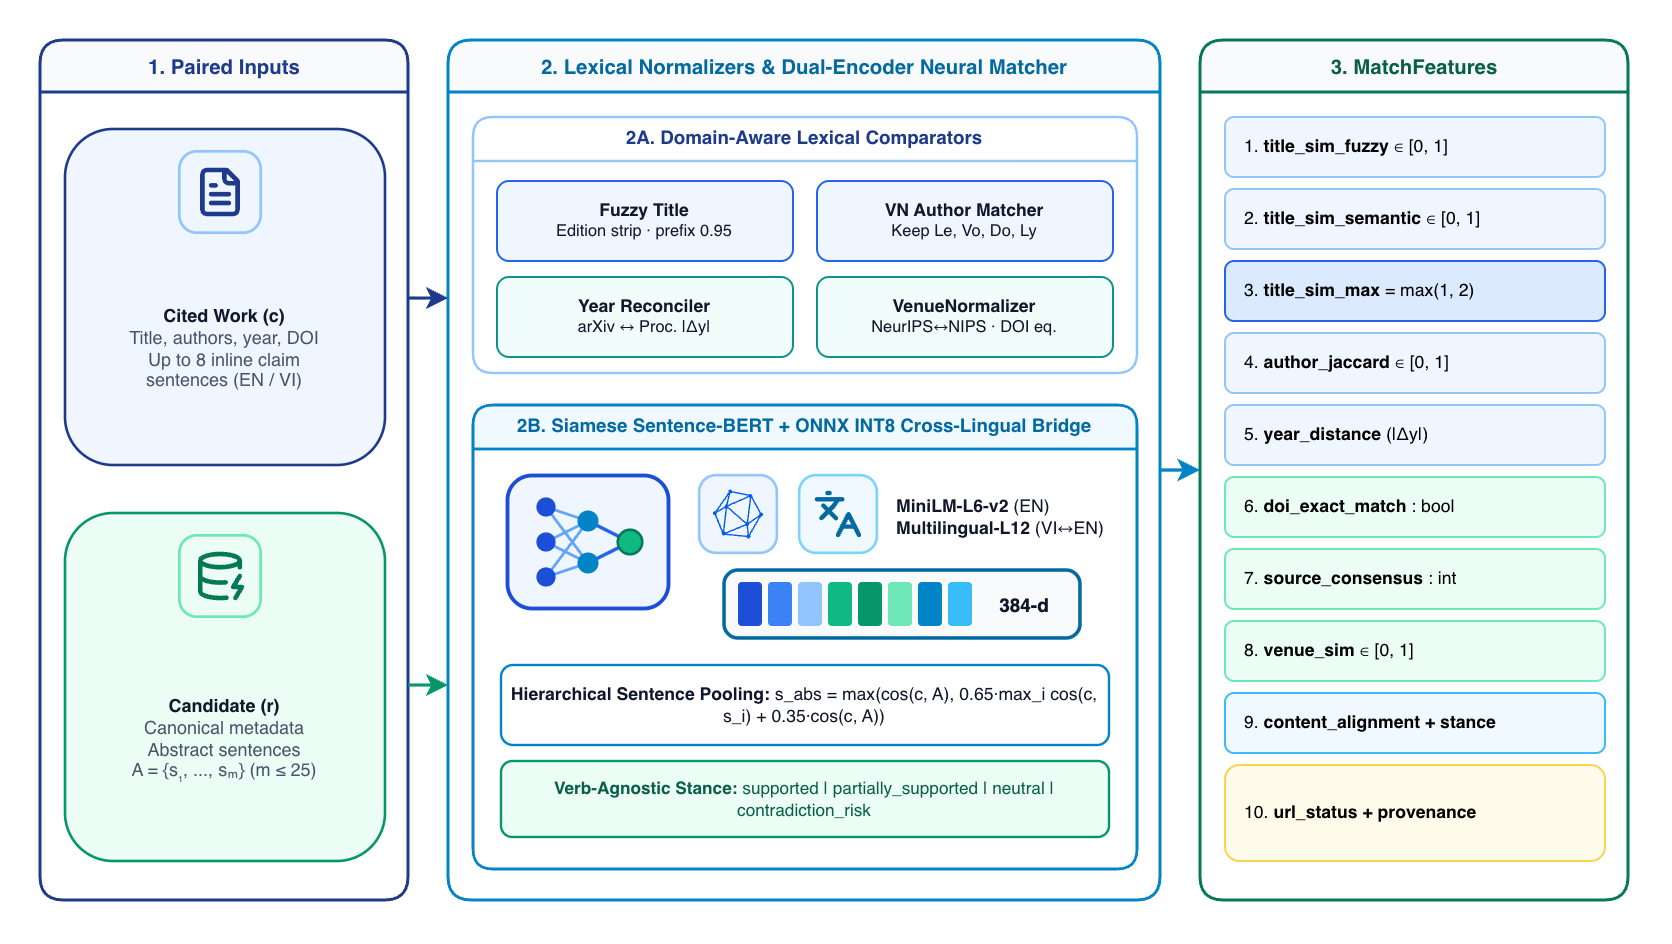
\includegraphics[width=\textwidth,keepaspectratio]{picture/figures/fig4_5_matching.png}
    \caption[Dual-encoder lexical, semantic, and cross-lingual matching architecture]{Matching layer architecture combining lexical field normalizers, Sentence-BERT sentence-pooled abstract alignment ($0.65\max + 0.35\text{abs}$), stance gating, and ONNX INT8 \texttt{VI}$\leftrightarrow$\texttt{EN} bridging.}
    \label{fig:matching}
\end{figure}

\section{Neuro-Symbolic Verification and Platt Calibration}

\subsection{Priority-Ordered Symbolic Decision Tree}

\texttt{NeuroSymbolicChecker} combines neural alignment features with a deterministic symbolic rule engine (\texttt{SymbolicRules}, containing \textbf{68 distinct \texttt{R-*} rule identifiers} across an Order 0 resource pre-screen and 16 priority-ordered scholarly rule groups) and a calibrated machine-learning scorer, as shown in Figure~\ref{fig:neurosymbolic} and detailed in Table~\ref{tab:rules}.

\begin{figure}[H]
    \centering
    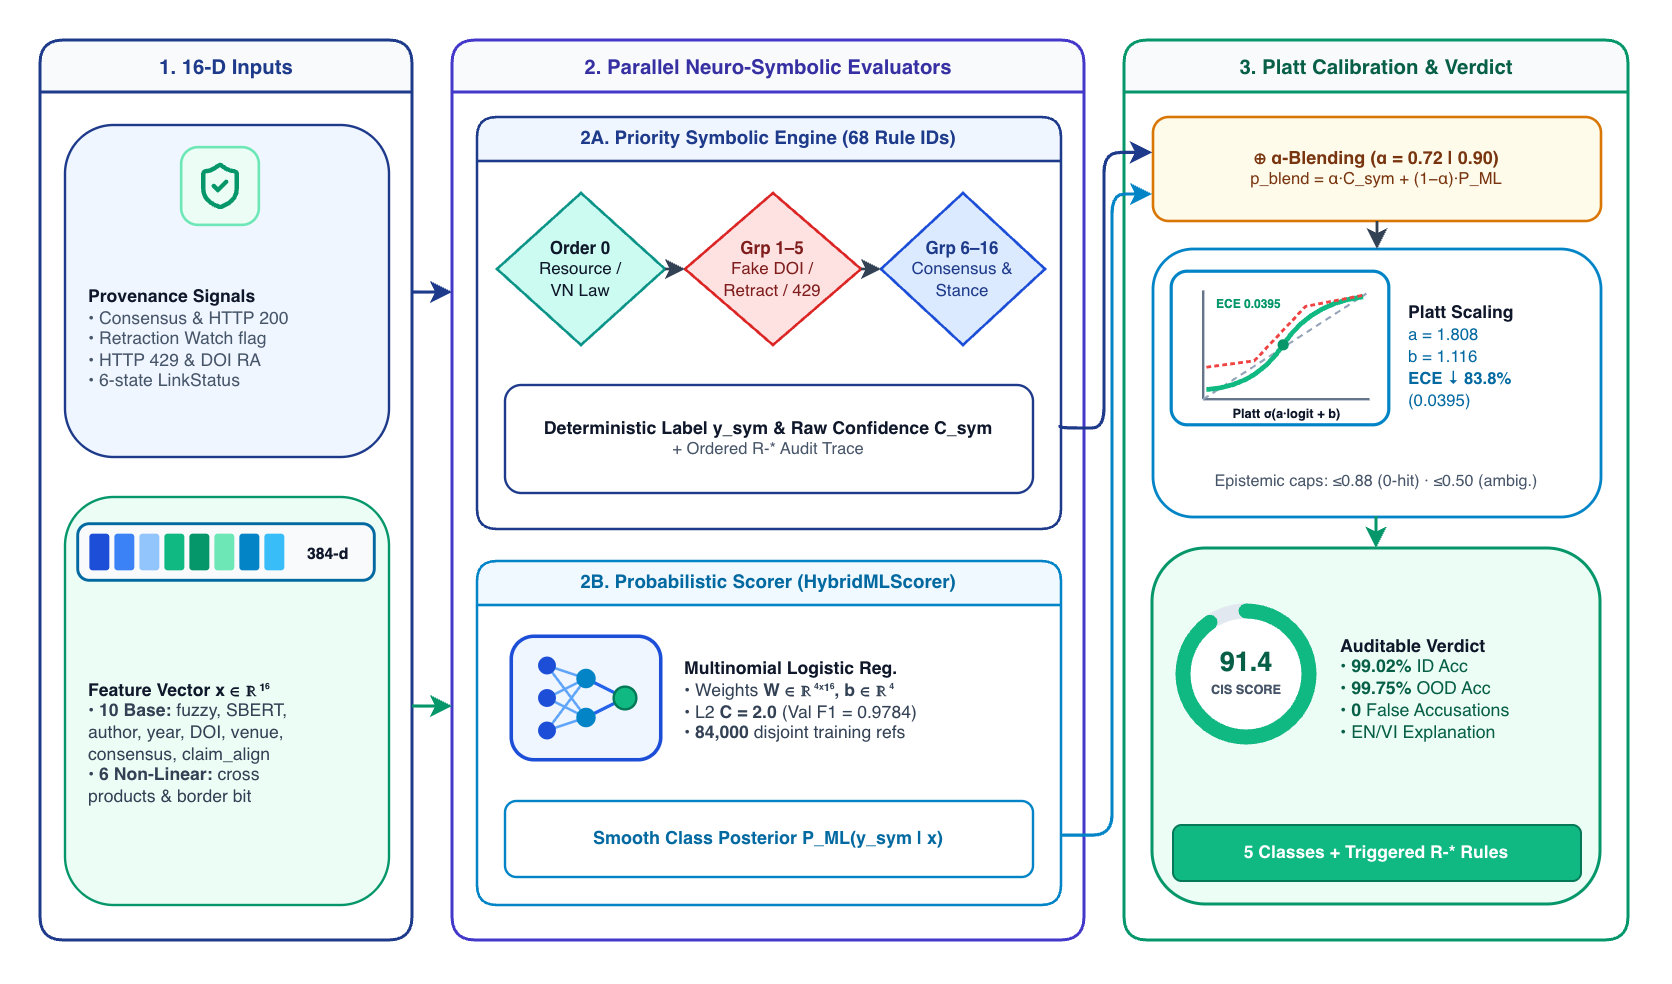
\includegraphics[width=\textwidth,keepaspectratio]{picture/figures/fig4_6_neurosymbolic.png}
    \caption[Neuro-symbolic verification engine and logit-space Platt calibration]{Neuro-symbolic verification architecture fusing the 16-group symbolic rule engine (68 rule IDs) with the 16-feature Multinomial Logistic Regression scorer and Platt calibrator.}
    \label{fig:neurosymbolic}
\end{figure}

{\setlength{\tabcolsep}{3.5pt}
\begin{longtable}{|C{0.11}|L{0.33}|L{0.56}|}
\caption{Evaluation order of symbolic pre-screening and the 16 verification rule groups (68 distinct \texttt{R-*} rule IDs).}\label{tab:rules}\\
\hline
\textbf{Group} & \textbf{Representative Rule ID(s)} & \textbf{Trigger Condition and Verdict Outcome} \\
\hline
\endfirsthead
\multicolumn{3}{c}{\itshape Table \thetable\ (continued from previous page)}\\
\hline
\textbf{Group} & \textbf{Representative Rule ID(s)} & \textbf{Trigger Condition and Verdict Outcome} \\
\hline
\endhead
\hline
\multicolumn{3}{r}{\itshape Continued on next page}\\
\endfoot
\hline
\endlastfoot
\textbf{Pre-0} & \texttt{R-URL-RESOURCE}, \texttt{R-WEB-RESOURCE}, \texttt{R-VN-LEGAL-VERIFIED}, \texttt{R-VN-LEGAL-\allowbreak MISMATCH} & Pure web documentation, software/RFC/HF artifact, or Vietnamese statute checked by \texttt{VNLegalVerifier} $\rightarrow$ \textbf{\texttt{resource}} (or \texttt{metadata\_error} if statutory authority/code conflicts). \\
\hline
\textbf{1} & \texttt{R-FAKE-URL}, \texttt{R-FABRICATED-DOI}, \texttt{R-CHIMERIC-DOI-\allowbreak MISMATCH}, \texttt{R-RETRACTED-PAPER} & RFC 2606 fake domain, unregistered DOI prefix, or real DOI resolving to an unrelated title $\rightarrow$ \textbf{\texttt{suspected\_hallucination}}; Retraction Watch flag (\texttt{is\_retracted}) $\rightarrow$ \textbf{\texttt{metadata\_error}}. \\
\hline
\textbf{2} & \texttt{R-FUTURE-YEAR}, \texttt{R-FUTURE-YEAR-\allowbreak KNOWN-AUTHOR} & Cited year exceeds current calendar year: unknown work $\rightarrow$ \textbf{\texttt{suspected\_hallucination}}; known work/author $\rightarrow$ \textbf{\texttt{metadata\_error}}. \\
\hline
\textbf{3} & \texttt{R-KNOWN-PAPER}, \texttt{R-TITLE-MISMATCH} & Matches 101-paper whitelist: full metadata \& stance agreement $\rightarrow$ \textbf{\texttt{verified}}; altered year/author/claim $\rightarrow$ \textbf{\texttt{metadata\_error}}. \\
\hline
\textbf{4} & \texttt{R-DEAD-URL}, \texttt{R-NONEXISTENT-DOI}, \texttt{R-NO-SCHOLARLY-\allowbreak RECORD} & Zero candidates while $\ge 2$ live registries returned clean HTTP 200 responses (or confirmed unarchived dead URL) $\rightarrow$ \textbf{\texttt{suspected\_hallucination}} (pure absence capped at $\le 0.88$). \\
\hline
\textbf{5} & \texttt{R-FAIL-ALL}, \texttt{R-RATE-LIMITED-\allowbreak ABSTAIN}, \texttt{R-DOI-RA-NO-CSL} & Zero candidates caused by HTTP 429 exhaustion, network outage, or valid regional DOI lacking public CSL metadata $\rightarrow$ \textbf{\texttt{unresolved}}. \\
\hline
\textbf{6} & \texttt{R-DOI-TITLE-AUTHOR} & Exact live DOI match with $\texttt{title\_sim} \ge 0.90$ and $\texttt{author\_jaccard} \ge 0.50$ $\rightarrow$ \textbf{\texttt{verified}}. \\
\hline
\textbf{7} & \texttt{R-LOCAL\_DB\_VERIFIED}, \texttt{R-LOCAL\_DB\_GOOD\_MATCH} & Offline FTS5 match ($\texttt{title\_sim\_fuzzy} \ge 0.95$, $\texttt{author\_jaccard} \ge 0.80$, $|\Delta y| = 0$) with no DOI conflict $\rightarrow$ \textbf{\texttt{verified}}. \\
\hline
\textbf{8} & \texttt{R-WELL-LINKED}, \texttt{R-WELL-LINKED-\allowbreak MODERATE} & Linked citation ($\texttt{matched}$) with strong title/author/year agreement and zero identifier contradiction $\rightarrow$ \textbf{\texttt{verified}}. \\
\hline
\textbf{9} & \texttt{R-DOI-TITLE-\allowbreak MISMATCH} & Live DOI resolves, but title similarity falls in $[0.60, 0.90)$ $\rightarrow$ \textbf{\texttt{metadata\_error}} with mismatched fields isolated. \\
\hline
\textbf{10} & \texttt{R-CONSENSUS-FULL}, \texttt{R-CONSENSUS-\allowbreak PARTIAL} & $\ge 2$ registries agree on title ($\ge 0.90$): matching author/year $\rightarrow$ \textbf{\texttt{verified}}; drifted author/year $\rightarrow$ \textbf{\texttt{metadata\_error}}. \\
\hline
\textbf{11} & \texttt{R-SINGLE-SOURCE-\allowbreak VERIFIED}, \texttt{R-BOOK-EDITION-\allowbreak VERIFIED}, \texttt{R-SINGLE-SOURCE-\allowbreak PARTIAL} & Single live registry match ($\ge 0.90$ title, $\ge 0.80$ author, $|\Delta y| \le 1$, or $\le 15\text{\,yr}$ across OpenLibrary book editions) $\rightarrow$ \textbf{\texttt{verified}}; field drift $\rightarrow$ \textbf{\texttt{metadata\_error}}. \\
\hline
\textbf{12} & \texttt{R-AMBIGUOUS-\allowbreak MAPPING} & Bipartite linker flagged \texttt{ambiguous\_mapping} $\rightarrow$ \textbf{\texttt{unresolved}} with confidence capped at $0.50$. \\
\hline
\textbf{13} & \texttt{R-CONTENT-\allowbreak ALIGNMENT}, \texttt{R-CONTENT-MISMATCH} & Strong context-to-abstract alignment rescues abbreviated titles ($\rightarrow$ \textbf{\texttt{verified}}); contradicted body claim on matched paper $\rightarrow$ \textbf{\texttt{metadata\_error}}. \\
\hline
\textbf{14} & \texttt{R-KNOWN-AUTHOR-\allowbreak TITLE-MISMATCH} & Known scholar combined with mismatched title in $[0.30, 0.90)$ $\rightarrow$ \textbf{\texttt{metadata\_error}}. \\
\hline
\textbf{15} & \texttt{R-ABSTENTION-\allowbreak BORDER}, \texttt{R-DOMAIN-EXCEPTION} & Borderline title similarity in $[0.40, 0.60)$ $\rightarrow$ \textbf{\texttt{unresolved}}; verified paper with dead external URL sets \texttt{domain\_exception = True}. \\
\hline
\textbf{16} & \texttt{R-WEAK-EVIDENCE}, \texttt{R-HALLUCINATED-\allowbreak SOURCE} & Terminal fallback ($\texttt{title\_sim} < 0.40$): $\ge 2$ clean live APIs + low author overlap $\rightarrow$ \textbf{\texttt{suspected\_hallucination}}; otherwise $\rightarrow$ \textbf{\texttt{unresolved}}. \\
\hline
\end{longtable}
}

Two provenance safeguards in \texttt{SymbolicRules} prevent overconfident false accusations. First, Group 4 (\texttt{R-NO-SCHOLARLY-RECORD}) fires only when at least two live scholarly APIs return HTTP 200 with zero matches; if APIs fail or hit HTTP 429, Group 5 forces \texttt{unresolved}. Second, when a hallucination suspicion rests purely on registry absence rather than a positive contradiction (such as a chimeric or fake DOI), post-calibration confidence is explicitly capped at $\le 0.88$ to acknowledge finite indexing coverage.

\subsection{16-Feature Logistic Regression and Platt Calibration}

To convert discrete symbolic outcomes into smooth, accurate probabilities, \texttt{HybridMLScorer} extracts a 16-dimensional feature vector $\mathbf{x} \in \mathbb{R}^{16}$ containing ten base features (\texttt{title\_sim\_fuzzy}, \texttt{title\_sim\_semantic}, \texttt{title\_sim\_max}, \texttt{author\_jaccard}, $\exp(-0.5 \min(|\Delta y|, 10))$, \texttt{doi\_exact\_match}, $\min(\text{consensus}, 4)/4$, \texttt{venue\_sim}, \texttt{content\_alignment\_signal}, \texttt{has\_candidate}) and six interaction terms (\texttt{title\_x\_author}, \texttt{title\_x\_year}, \texttt{title\_mismatch\_author}, \texttt{title\_mismatch\_year}, \texttt{doi\_mismatch\_title}, and \texttt{abstention\_zone\_indicator}).

A Multinomial Logistic Regression model ($W \in \mathbb{R}^{4 \times 16}, \mathbf{b} \in \mathbb{R}^4$, regularized at $C = 0.25$ with balanced class weights on 84,000 disjoint training citations) outputs $P_{\text{ML}}(y \mid \mathbf{x})$. In \texttt{SymbolicRules}, provenance modifiers (\texttt{R-LOCAL\_DB}: $-0.05$, \texttt{R-API\_EXHAUSTED}: $-0.10$, \texttt{R-LOCAL\_DB\_ONLY}: $-0.15$) first adjust local-only or rate-limited symbolic confidence; \texttt{HybridMLScorer} then blends symbolic confidence $C_{\text{sym}}^{(0)}$ with $P_{\text{ML}}(y_{\text{sym}} \mid \mathbf{x})$ via Equation~\eqref{eq:platt-calib} using $\alpha = 0.72$ (raised automatically to $\alpha = 0.90$ when $C_{\text{sym}}^{(0)} \ge 0.85$ and $|C_{\text{sym}}^{(0)} - P_{\text{ML}}| > 0.45$ so symbolic guardrails on retracted or fake-URL citations are never diluted). Finally, \texttt{PlattCalibrator} ($a = 1.891263, b = 1.138599$, fitted on 18,000 validation citations), document style penalties, and the $\le 0.88$ pure-absence cap produce the final calibrated confidence.

\section{Integrity Scoring and Bilingual Explanations}

\subsection{Five-Component Citation Integrity Score}

\texttt{CISCalculator.compute()} summarizes manuscript-wide citation quality as an interpretable score in $[0, 100]$. Non-scholarly \texttt{resource} entries are excluded from the academic denominator $N_{\text{acad}}$ so citing official software manuals or national laws never distorts scholarly verification ratios. For $N_{\text{acad}} \ge 1$, \texttt{metadata\_accuracy} ($s_{\text{meta}}$) applies tiered deductions across standard metadata errors ($N_{\text{meta\_std}}$, penalty $0.50$), severely incomplete references ($N_{\text{meta\_incomp}}$, penalty $0.75$), and suspected hallucinations ($N_{\text{hall}}$, penalty $1.00$), as defined in Equation~\eqref{eq:cis-meta}:
\begin{equation}\label{eq:cis-meta}
s_{\text{meta}} = \max\left(0,\; 1 - \frac{0.50\,N_{\text{meta\_std}} + 0.75\,N_{\text{meta\_incomp}} + 1.00\,N_{\text{hall}}}{N_{\text{acad}}}\right).
\end{equation}
Combining all five components in Table~\ref{tab:cis} produces the final Citation Integrity Score in Equation~\eqref{eq:cis-total}:
\begin{equation}\label{eq:cis-total}
\text{CIS} = 100 \times \bigl(0.35\,s_{\text{ver}} + 0.25\,s_{\text{meta}} + 0.25\,s_{\text{link}} + 0.10\,s_{\text{fmt}} + 0.05\,s_{\text{id}}\bigr).
\end{equation}

{\setlength{\tabcolsep}{3.5pt}
\begin{longtable}{|L{0.31}|C{0.11}|L{0.58}|}
\caption{Components and default rubric weights of the Citation Integrity Score (CIS).}\label{tab:cis}\\
\hline
\textbf{Component} & \textbf{Weight} & \textbf{Exact Definition in \texttt{CISCalculator.compute()}} \\
\hline
\endfirsthead
\multicolumn{3}{c}{\itshape Table \thetable\ (continued from previous page)}\\
\hline
\textbf{Component} & \textbf{Weight} & \textbf{Exact Definition in \texttt{CISCalculator.compute()}} \\
\hline
\endhead
\hline
\multicolumn{3}{r}{\itshape Continued on next page}\\
\endfoot
\hline
\endlastfoot
\textbf{\texttt{verified\_ratio}} ($s_{\text{ver}}$) & \textbf{0.35} & $N_{\text{verified}} / N_{\text{acad}}$, measuring corroborated scholarly references. \\
\hline
\textbf{\texttt{metadata\_accuracy}} ($s_{\text{meta}}$) & \textbf{0.25} & Tiered bibliographic fidelity score defined in Equation~\eqref{eq:cis-meta}. \\
\hline
\textbf{\texttt{in\_text\_bib\_consistency}} ($s_{\text{link}}$) & \textbf{0.25} & One minus the weighted linking penalties (Table~\ref{tab:mapping-statuses}) across inline links, uncited entries, and duplicates. \\
\hline
\textbf{\texttt{format\_consistency}} ($s_{\text{fmt}}$) & \textbf{0.10} & Document style consistency derived from \texttt{StyleProfile} and per-entry style deviations. \\
\hline
\textbf{\texttt{identifier\_validity}} ($s_{\text{id}}$) & \textbf{0.05} & Share of DOI/URL-bearing citations whose identifiers resolve cleanly without \texttt{dead\_link}, \texttt{fake\_domain}, or \texttt{domain\_exception}. \\
\hline
\end{longtable}
}

\subsection{Bilingual Verdict Explanations and Bibliography Repair}

Every verdict is accompanied by a deterministic English and Vietnamese explanation (\texttt{logic/explanation.py} and \texttt{verdictExplanation.ts}) reporting the matched registry, field-level diffs, semantic alignment score, and triggered rule IDs. For entries labeled \texttt{metadata\_error} or \texttt{verified}, the remediation modules (\texttt{export/bibliography\_formatter.py} and \texttt{export/docx\_exporter.py}) reconstruct clean APA 7th, IEEE, TDTU, BibTeX, and RIS strings from canonical registry fields and export a repaired \texttt{.docx} manuscript while leaving \texttt{suspected\_hallucination} entries highlighted for author removal.

\section{Web Presentation Layer (CITRA)}

\subsection{Frontend Architecture and Progressive Disclosure}

The web client (\textbf{CITRA}) is implemented in React 18.3, TypeScript 5.8, Vite, TanStack React Query, and Tailwind CSS v3.4. Both Light (\texttt{\#FBFAF6}) and Dark (\texttt{\#13120F}) themes satisfy WCAG 2.1 AA contrast ratios and support full Vietnamese diacritic typography. To serve both non-technical students and software engineering auditors, the UI applies \emph{progressive disclosure}: primary cards display plain-language verdicts and repair actions, whereas raw symbolic rule codes (\texttt{R-*}), feature vectors, and 5-stage execution traces expand on demand via accessible \texttt{aria-expanded} drawers. Rollup code-splitting keeps the entry bundle at $228.42\text{\,kB}$ ($66.39\text{\,kB}$ gzipped), with all 60 lazy-loaded route chunks $\le 251.00\text{\,kB}$.

\subsection{Role-Based Workspaces and Telemetry Surfaces}

Figures~\ref{fig:ui-landing}--\ref{fig:ui-portals} showcase the live \texttt{v3.90.9} interface across unauthenticated and role-gated routes. Figure~\ref{fig:ui-landing} illustrates the public landing page in Light and Dark themes. Figure~\ref{fig:ui-workspace} shows the Student/Researcher dashboard and the multi-file batch verification queue (\texttt{.pdf}, \texttt{.docx}, \texttt{.bib}, \texttt{.ris}) supporting concurrent classroom uploads. Figure~\ref{fig:ui-portals} displays the Teacher Classroom cohort analytics view (highlighting grade band histograms and cross-student shared hallucinations) alongside the Administrator System Health console monitoring GROBID, SQLite FTS5, and all fifteen upstream API circuit breakers.

\begin{figure}[H]
    \centering
    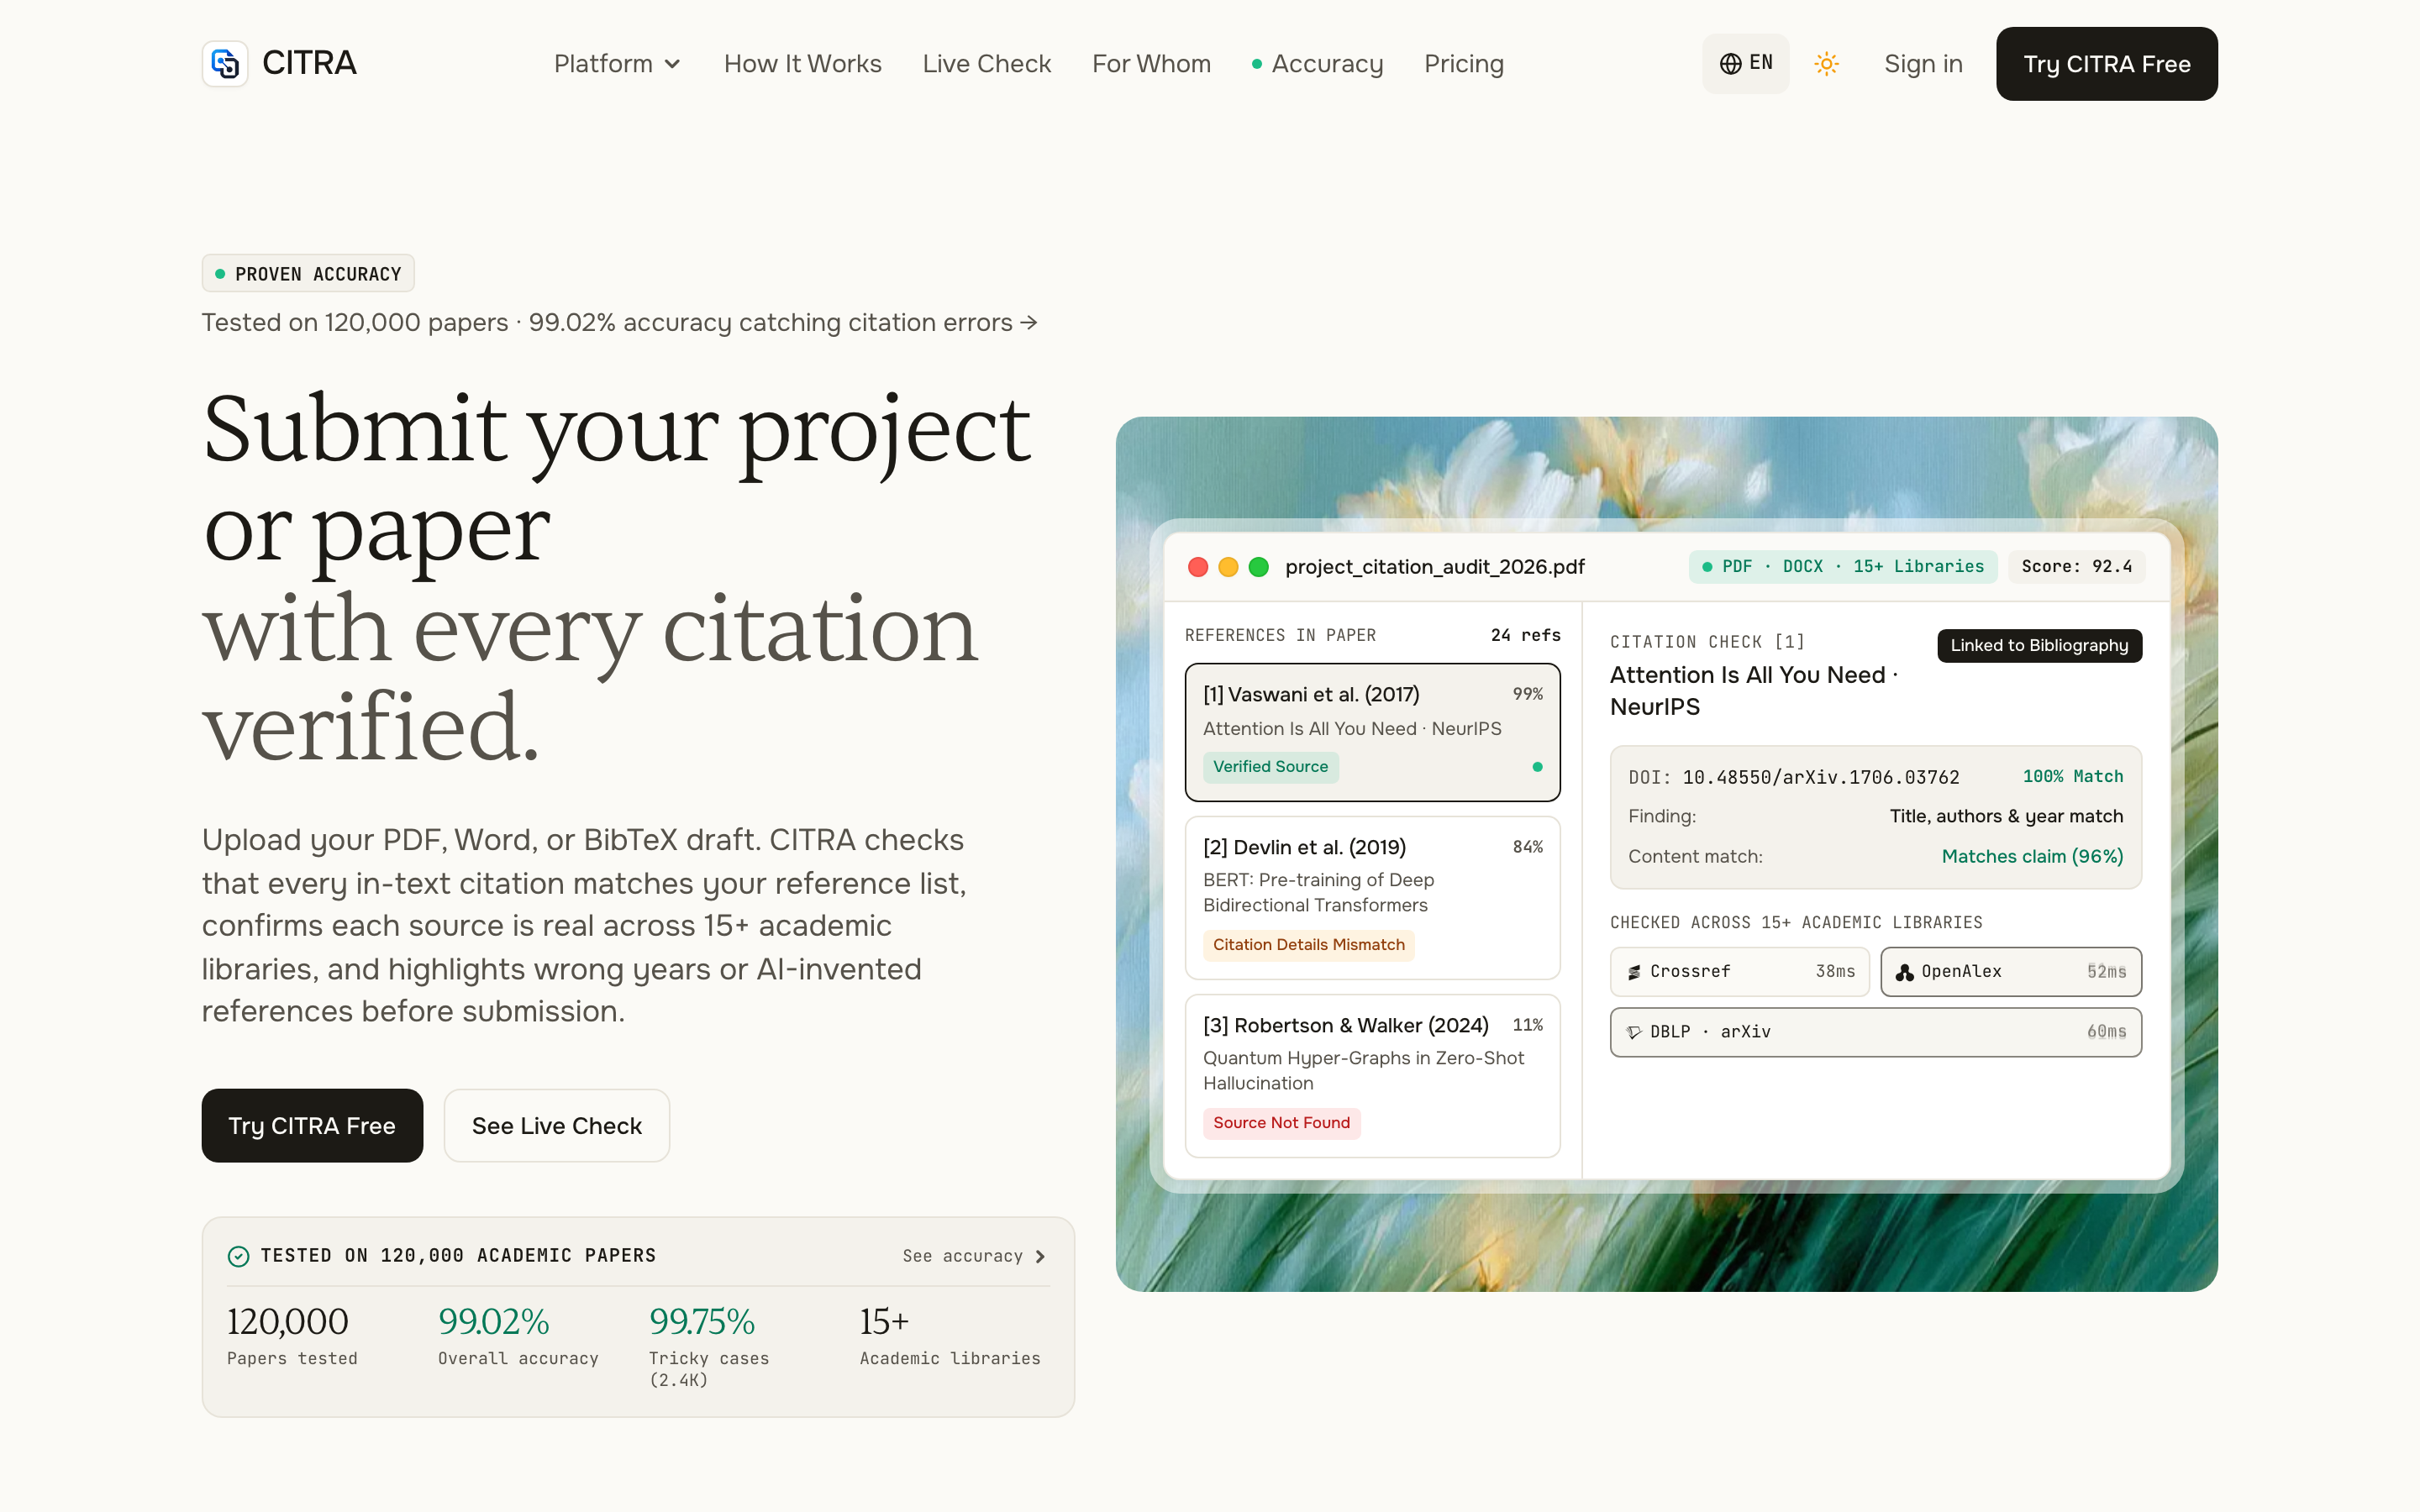
\includegraphics[width=0.49\textwidth,keepaspectratio]{picture/figures/01-landing-light.png}\hfill
    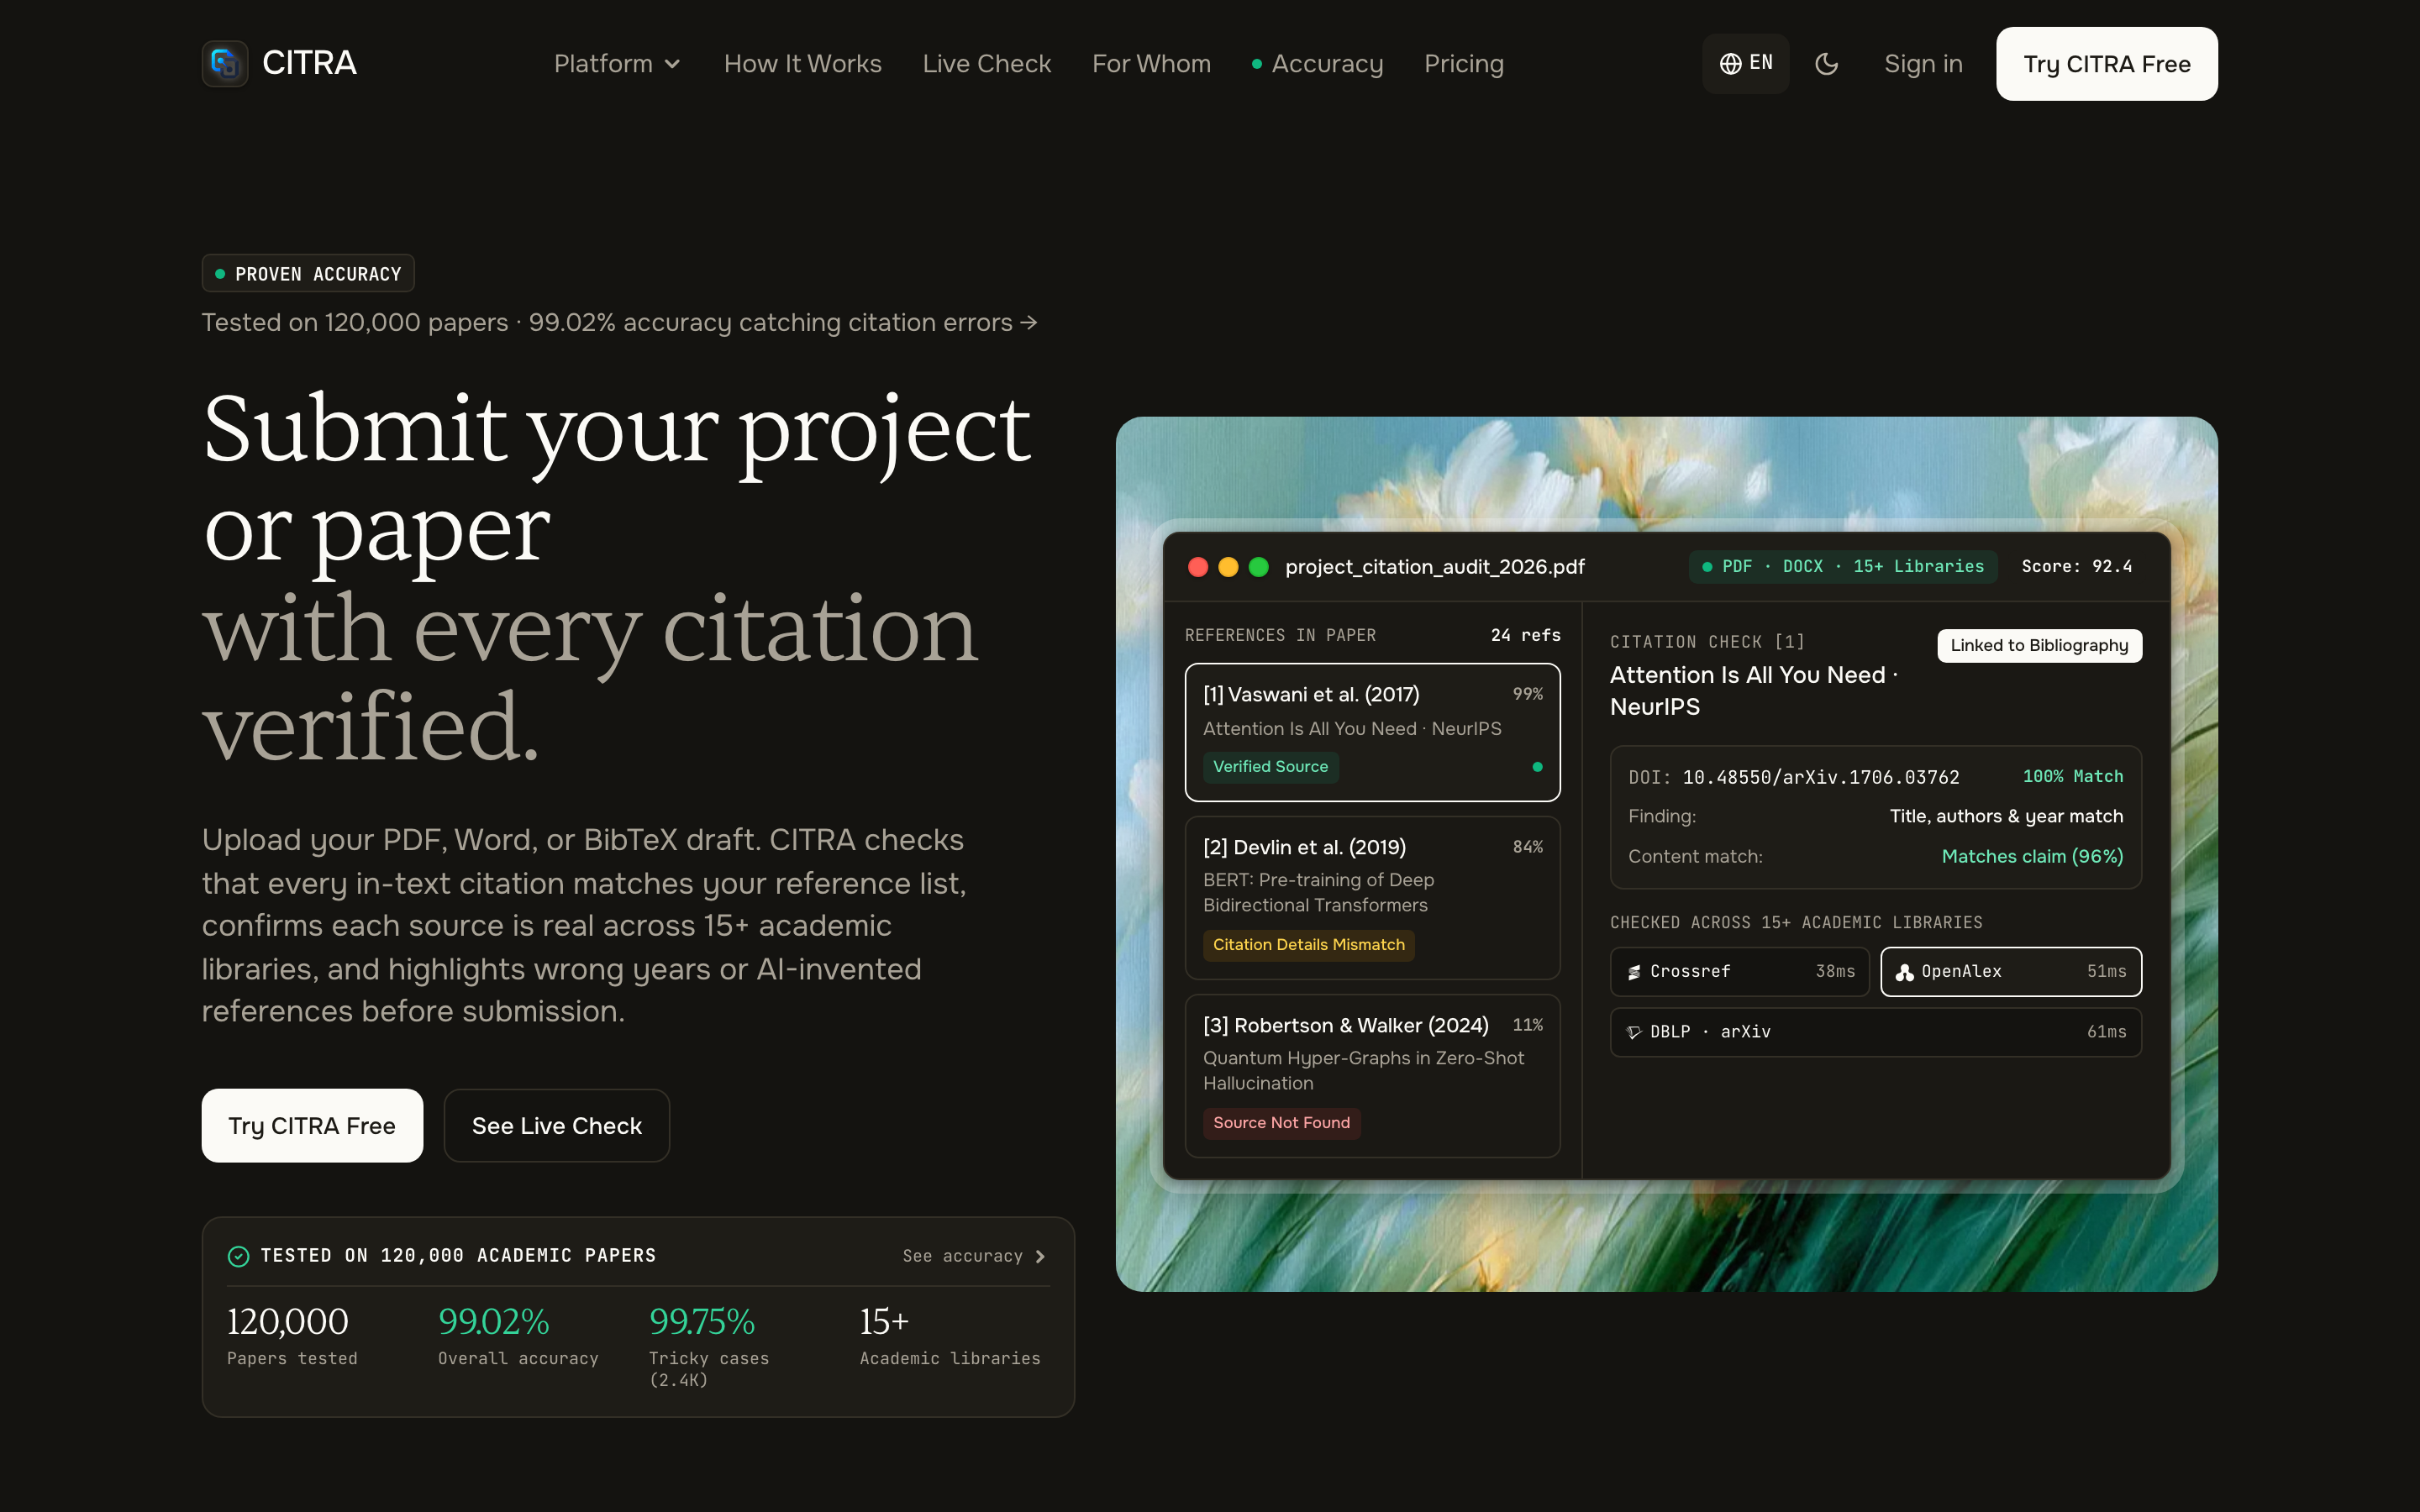
\includegraphics[width=0.49\textwidth,keepaspectratio]{picture/figures/02-landing-dark.png}
    \caption[CITRA landing page in WCAG AA Light and Dark themes]{CITRA (\texttt{v3.90.9}) public landing page rendered in Light mode (left) and Dark mode (right).}
    \label{fig:ui-landing}
\end{figure}

\begin{figure}[H]
    \centering
    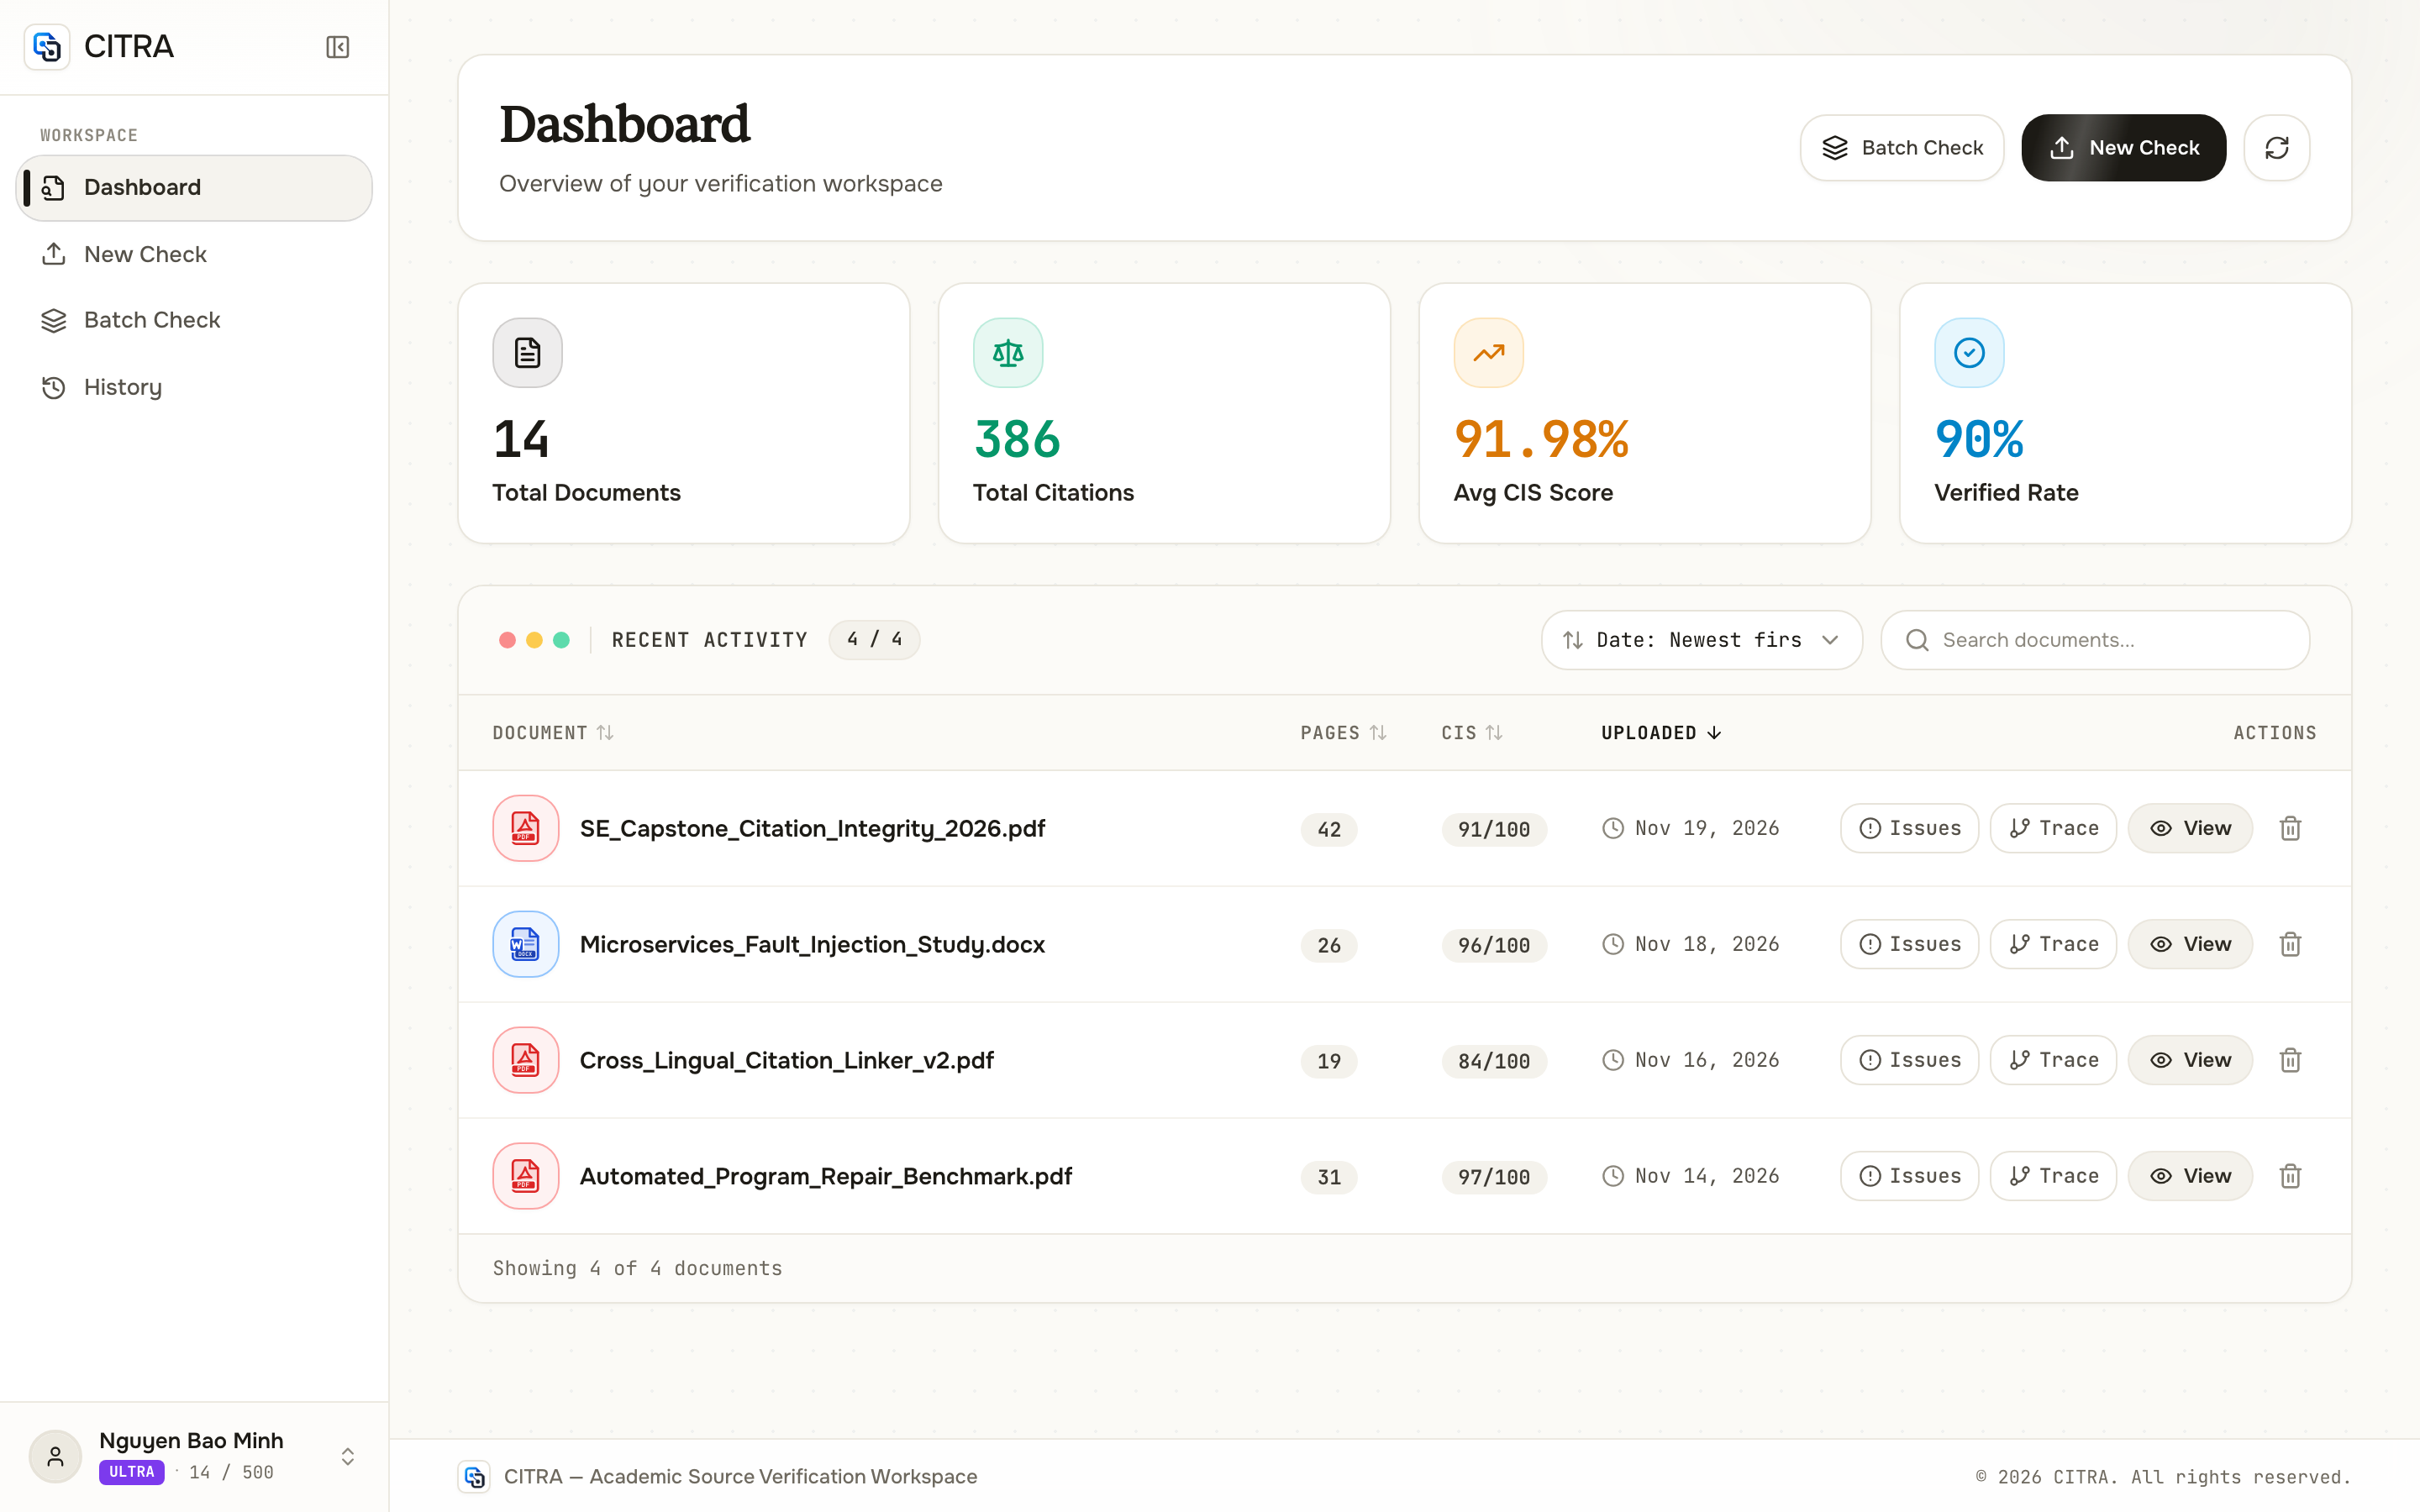
\includegraphics[width=0.49\textwidth,keepaspectratio]{picture/figures/03-dashboard-light.png}\hfill
    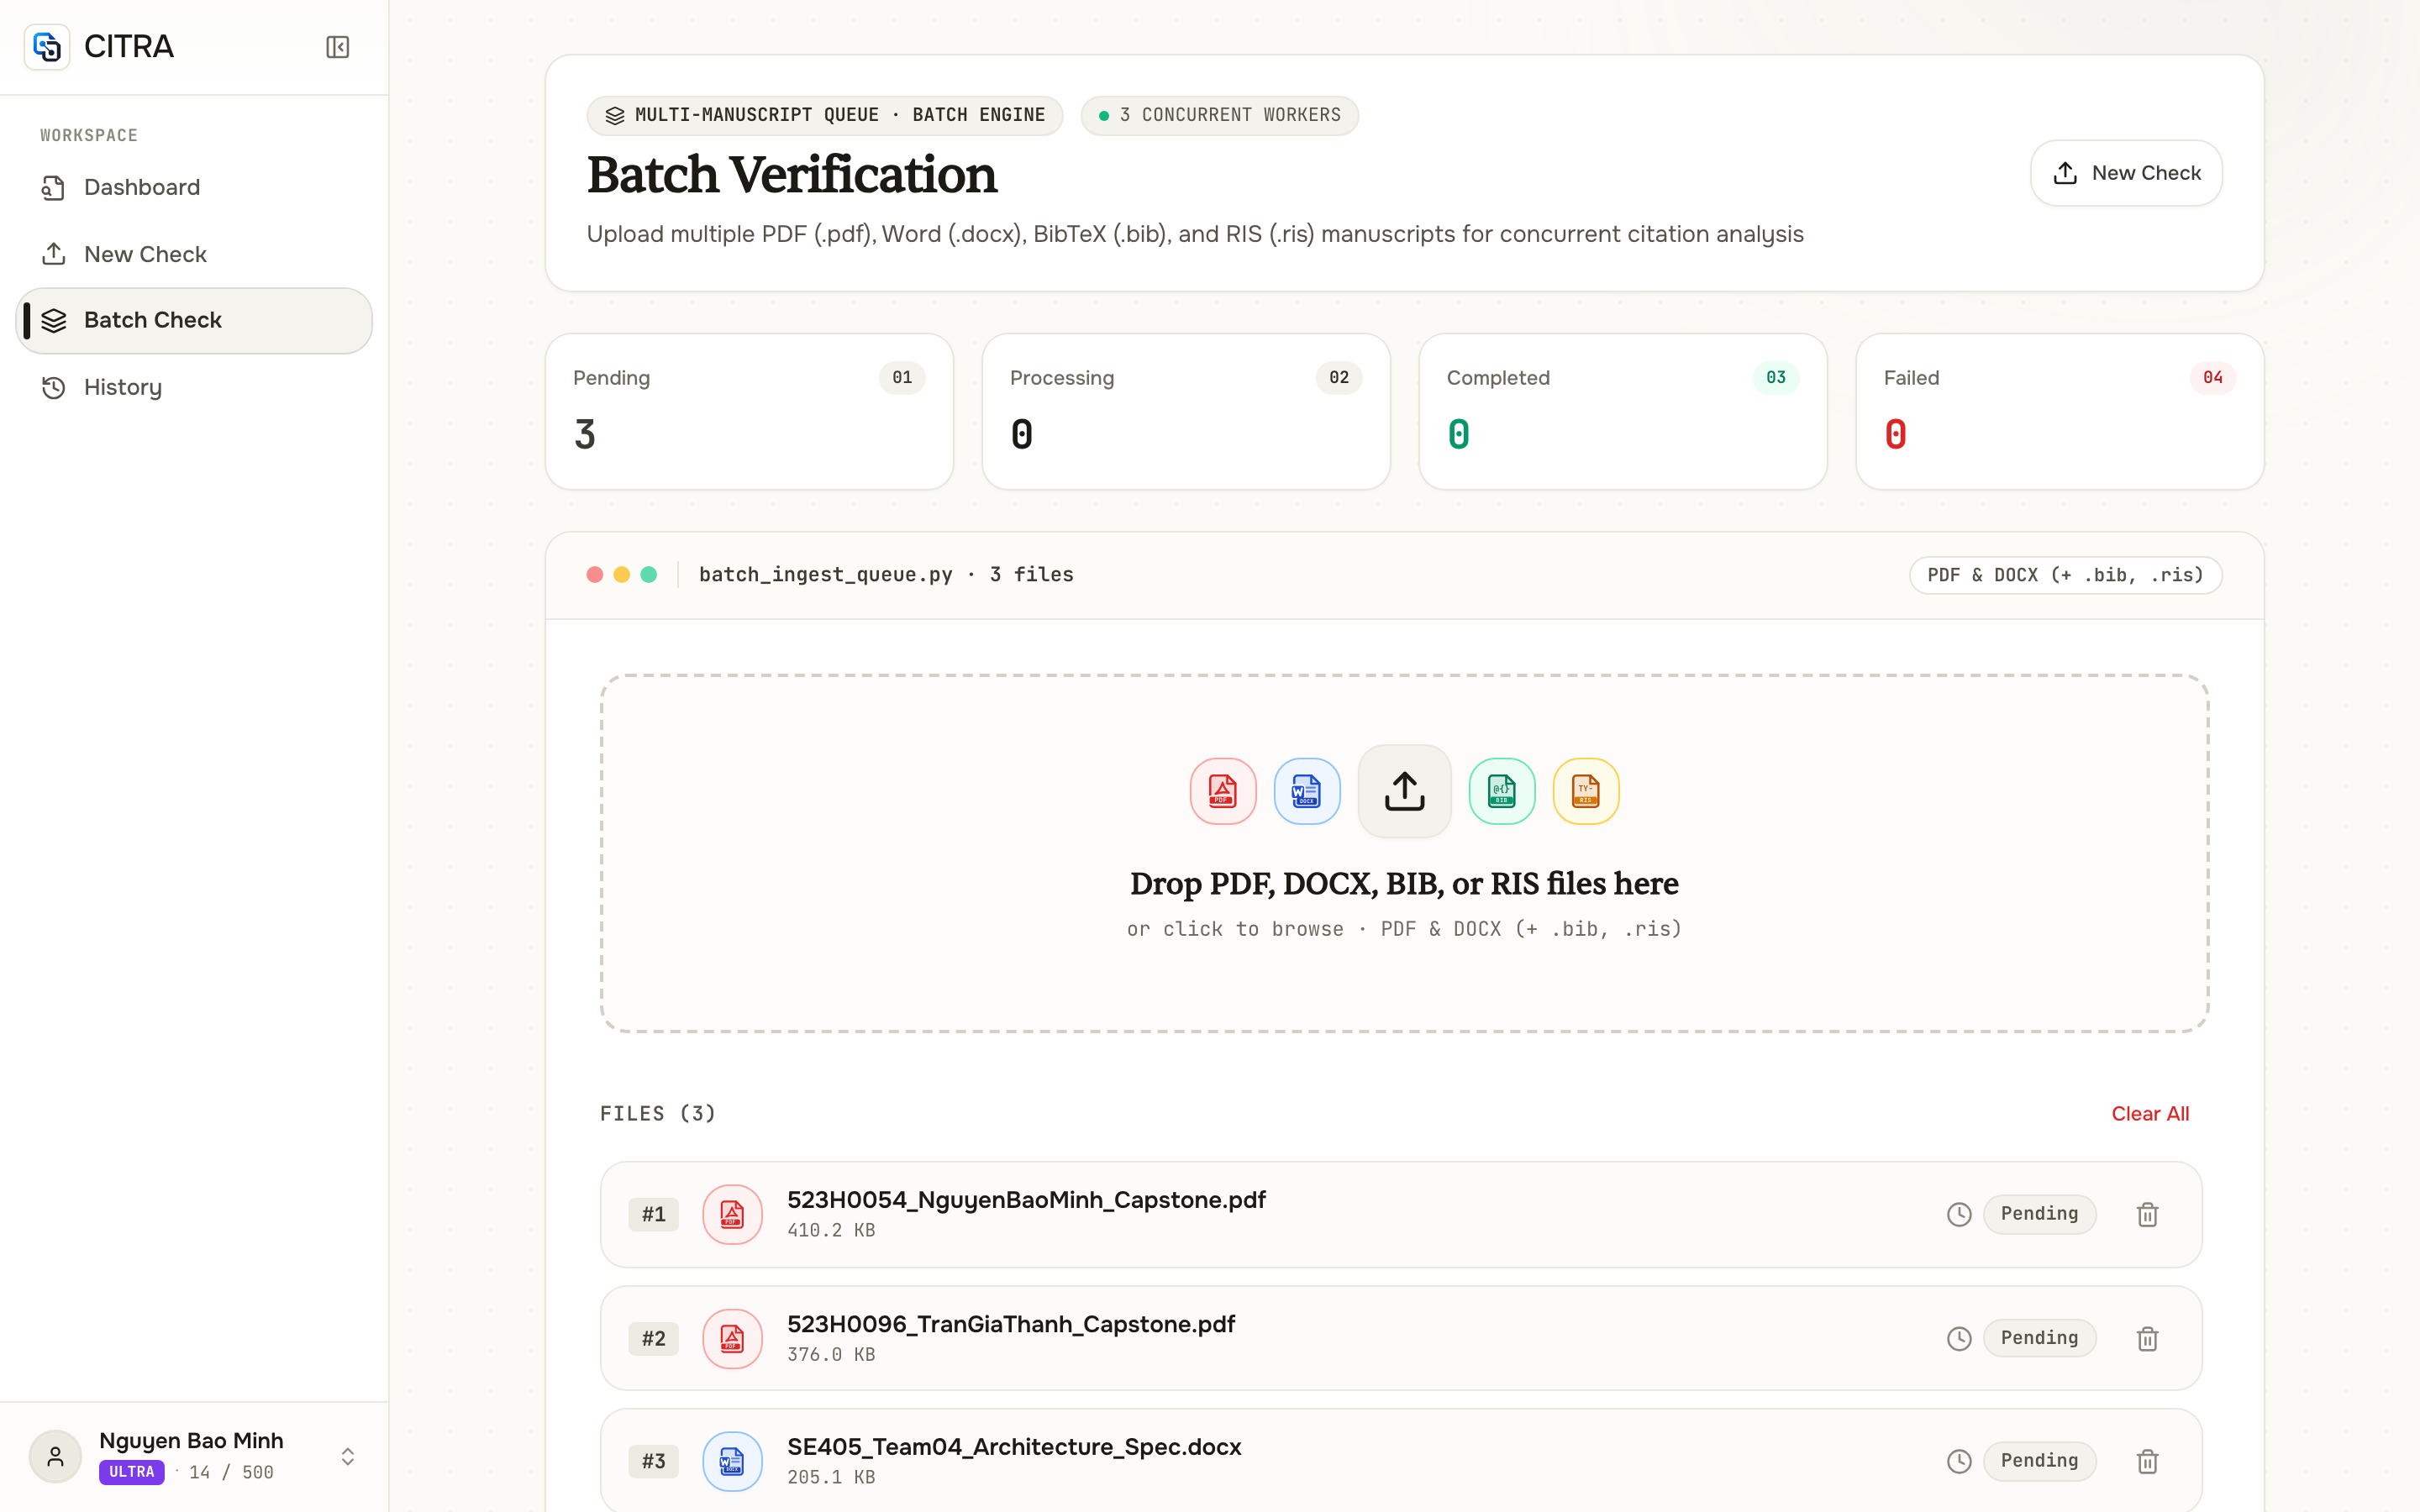
\includegraphics[width=0.49\textwidth,keepaspectratio]{picture/figures/04-batch-upload.png}
    \caption[Student verification dashboard and concurrent batch upload workspace]{Student verification dashboard (\texttt{/dashboard}, left) and multi-format batch verification queue (\texttt{/batch-upload}, right).}
    \label{fig:ui-workspace}
\end{figure}

\begin{figure}[H]
    \centering
    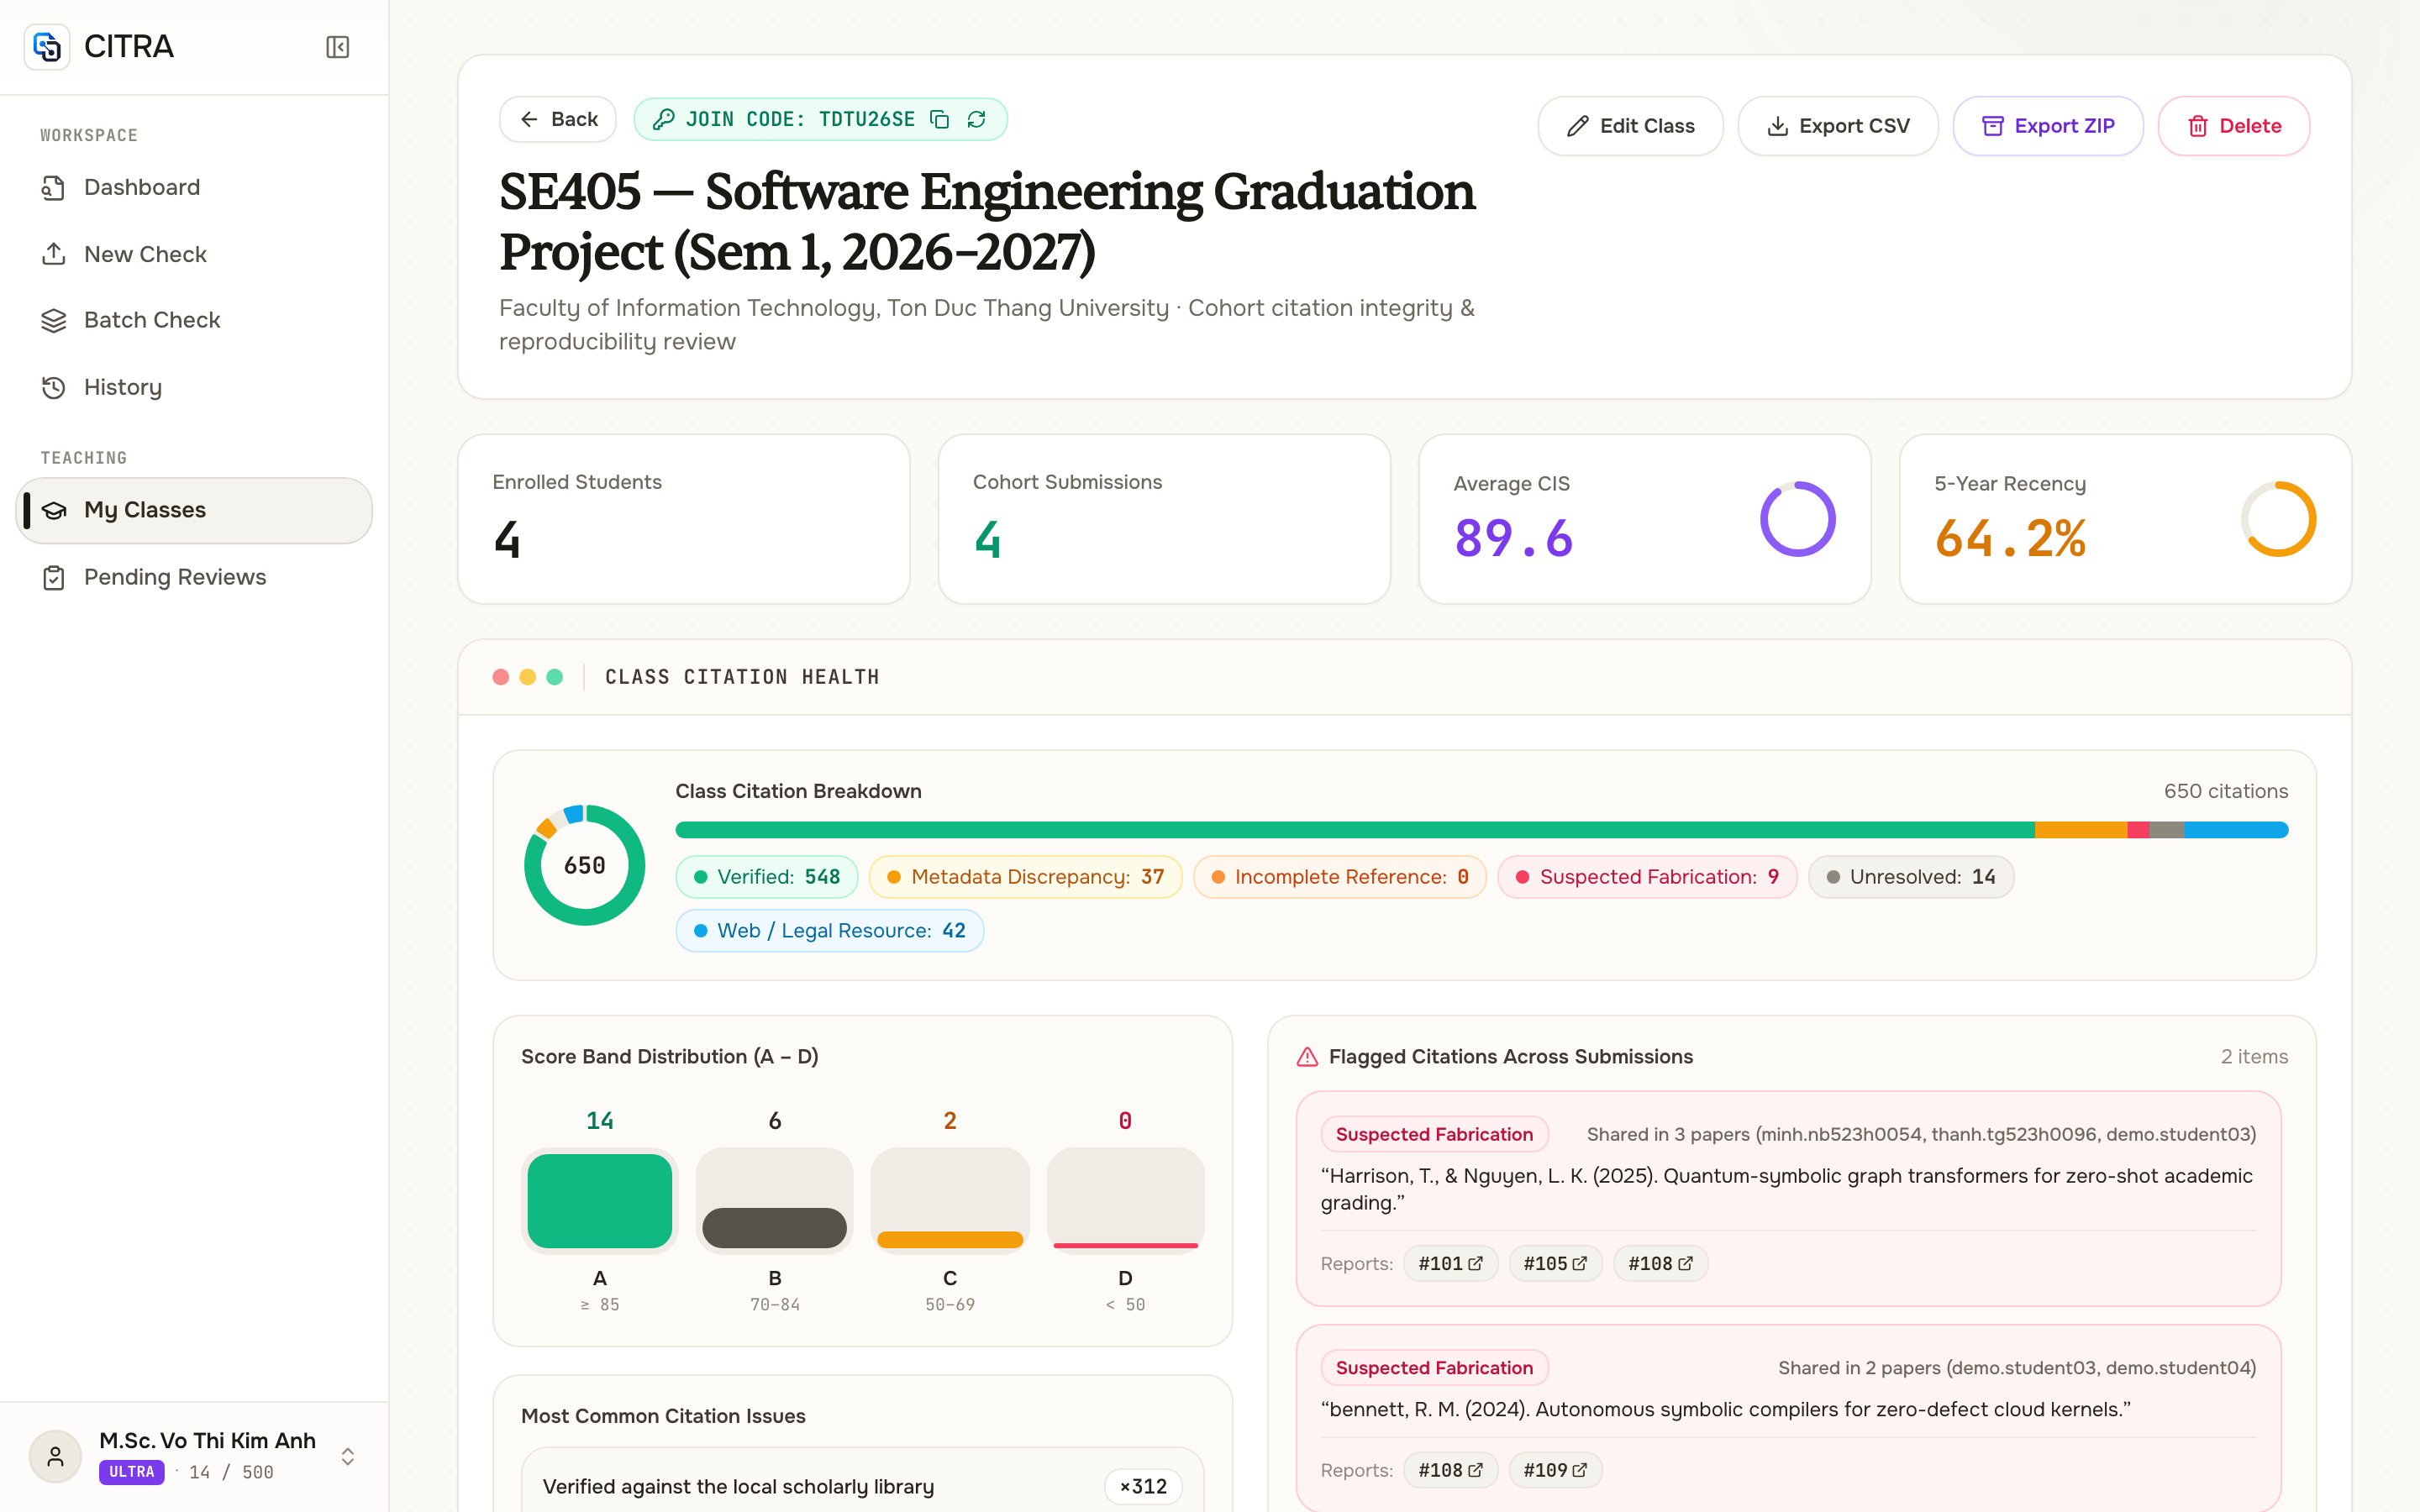
\includegraphics[width=0.49\textwidth,keepaspectratio]{picture/figures/10-teacher-classroom.png}\hfill
    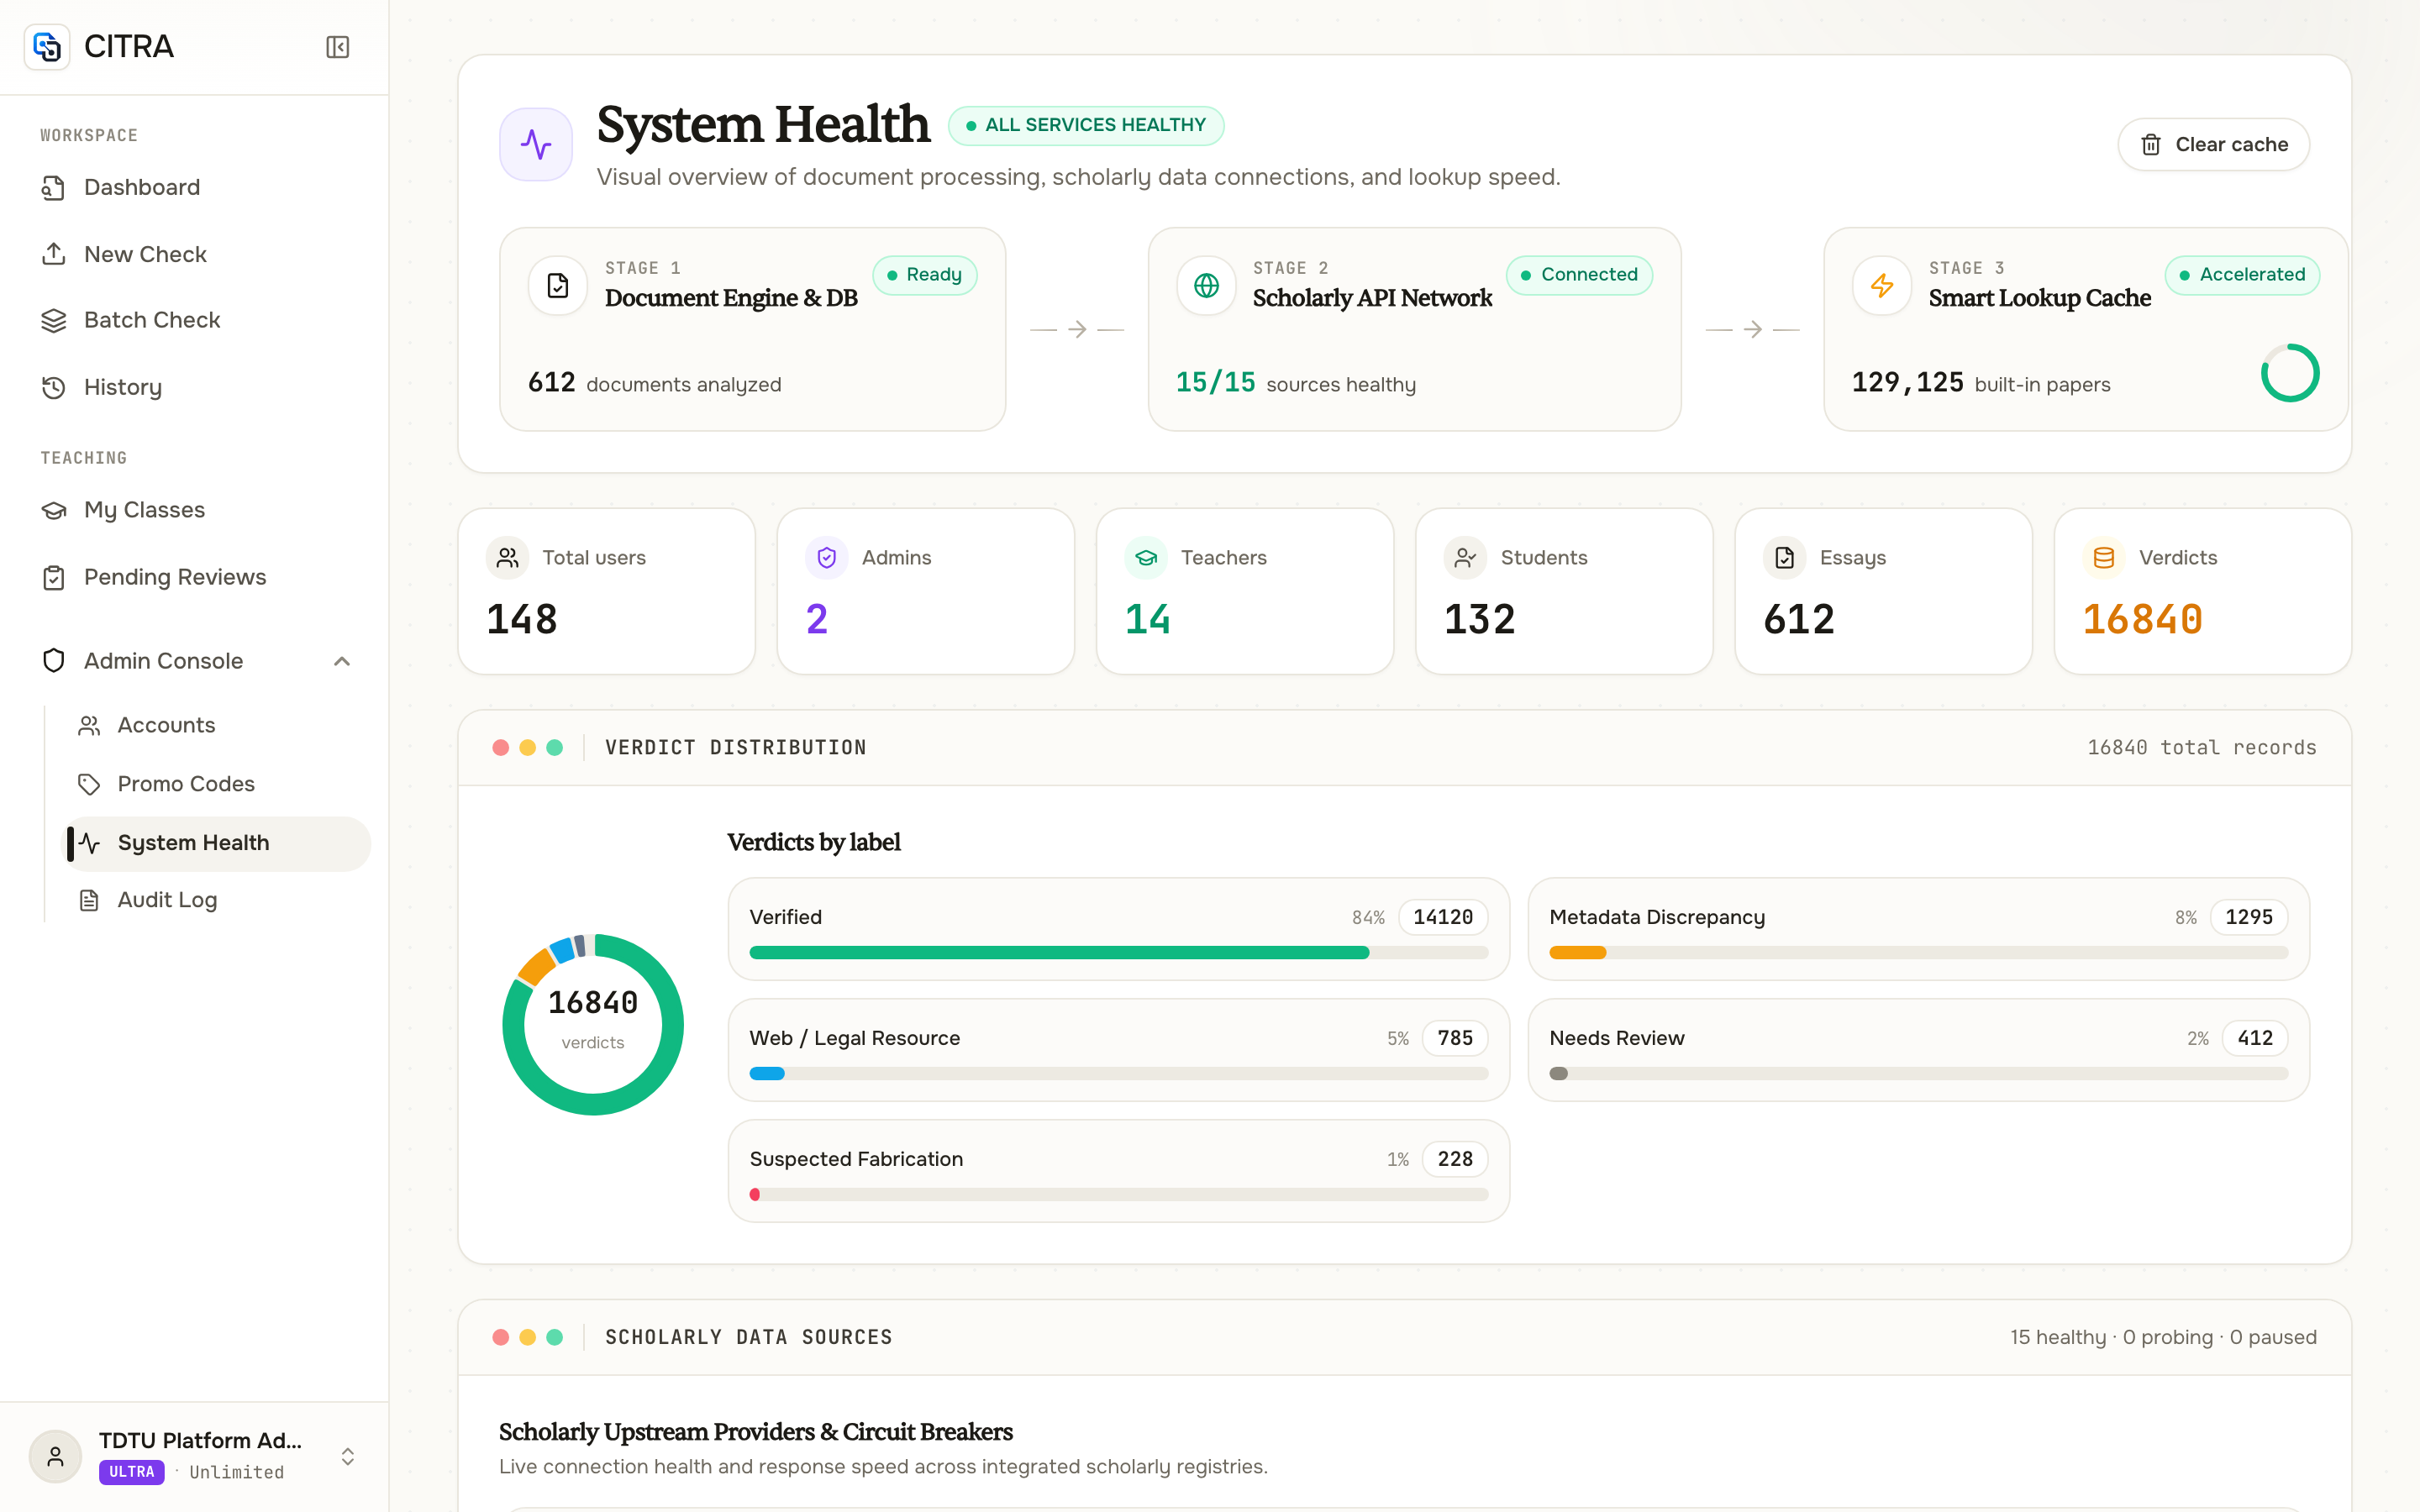
\includegraphics[width=0.49\textwidth,keepaspectratio]{picture/figures/11-admin-system-health.png}
    \caption[Teacher cohort analytics classroom and Administrator system health console]{Teacher classroom cohort analytics (\texttt{/teacher/classes/1}, left) and Administrator system health monitor (\texttt{/admin/system}, right).}
    \label{fig:ui-portals}
\end{figure}

\section{Chapter Summary}

This chapter presented the implementation of \textbf{CITRA} across its eight software layers: multi-format 12-style extraction, work-level merging and 7-method bidirectional linking, tiered 15-API retrieval with pinned-IP URL/HTML validation, dual-encoder \texttt{VI}$\leftrightarrow$\texttt{EN} semantic matching, 68-rule neuro-symbolic verification with 16D Logistic Regression and Platt scaling, five-component CIS grading, and the code-split React workspace. Chapter~\ref{chap:results} evaluates these components empirically across five research questions.


\newpage
\chapter{System Verification and Experimental Results}
\label{chap:results}

\section{Experimental Design and Verification Setup}

Following Empirical Software Engineering evaluation standards~\cite{wohlin2012experimentation}, this chapter evaluates \textbf{CITRA} (\texttt{v3.90.7}) through automated unit, integration, and browser test suites, requirements traceability verification, and controlled quantitative benchmarks structured around five Research Questions (\textbf{RQ1}--\textbf{RQ5}).

\subsection{Research Questions}

\begin{itemize}
    \item \textbf{RQ1 (In-Distribution Accuracy and Ablation):} How accurately does the proposed neuro-symbolic engine classify citations on a leak-free, paper-disjoint benchmark compared with single-source, lexical, neural, and pure machine-learning baselines (\texttt{B0}--\texttt{B5})?
    \item \textbf{RQ2 (Out-of-Distribution Symbolic Robustness):} How effectively do symbolic guardrails handle discrete integrity violations (retracted papers, chimeric DOIs, placeholder URLs, regional DOIs, API rate limits, and statutory mismatches) where continuous linear classifiers fail?
    \item \textbf{RQ3 (Probability Calibration and CIS Stability):} Does logit-space Platt scaling improve confidence calibration and selective risk-coverage trade-offs, and how stable are Citation Integrity Score (CIS) manuscript rankings under rubric weight perturbations?
    \item \textbf{RQ4 (Multi-Domain and Real Manuscript Generalization):} Does the end-to-end pipeline generalize across raw multi-domain references, multi-style academic PDFs, Vietnamese legal corpora, and real undergraduate capstone reports?
    \item \textbf{RQ5 (Latency, Caching, and Concurrency Scalability):} Does the platform satisfy all non-functional latency, memory, and 50-user deadline burst SLAs on standard CPU hardware?
\end{itemize}

\subsection{Automated Test Suites and Requirements Traceability Matrix}

Software verification spans three automated test layers summarized in Table~\ref{tab:test-suites}: 2,410+ passing backend \texttt{pytest} unit and integration tests (with environment-gated live-network skips and 0 failures), 488 passing frontend \texttt{Vitest} tests across 63 suites, and 20 \texttt{Playwright} end-to-end browser specification suites across desktop, tablet, and mobile viewports. In addition, an offline retrieval test over 500 stratified ACL Anthology queries achieved $99.80\%$ recall ($499/500$) and $100.0\%$ precision at $87.62\text{\,ms}$ mean latency. Table~\ref{tab:rtm} provides the bidirectional Requirements Traceability Matrix (RTM) linking the functional and non-functional specifications from Chapter~\ref{chap:overview} to their implementing packages and verification evidence.

{\setlength{\tabcolsep}{3.5pt}
\begin{longtable}{|L{0.23}|L{0.25}|L{0.52}|}
\caption{Automated software verification suites executed in version \texttt{3.90.7}.}\label{tab:test-suites}\\
\hline
\textbf{Verification Layer} & \textbf{Execution Result} & \textbf{Verified Subsystem Scope} \\
\hline
\endfirsthead
\multicolumn{3}{c}{\itshape Table \thetable\ (continued from previous page)}\\
\hline
\textbf{Verification Layer} & \textbf{Execution Result} & \textbf{Verified Subsystem Scope} \\
\hline
\endhead
\hline
\multicolumn{3}{r}{\itshape Continued on next page}\\
\endfoot
\hline
\endlastfoot
\textbf{Backend (\texttt{pytest})} & \textbf{2,410+ passed (0 failed)} & Multi-format extraction, 12 styles, \texttt{VNLegalVerifier}, 7-method linker, FTS5 + 15 APIs, SSRF-safe URL/HTML checks, 68 symbolic rules, Platt calibration, CIS, RBAC/IDOR, migrations \texttt{0001}--\texttt{0013}, and crash recovery. \\
\hline
\textbf{Frontend (\texttt{Vitest})} & \textbf{488 passed (63 suites, 0 failed)} & Auth/OAuth flows, progressive-disclosure drawers, 6 diagnostic report views, Citation Network DAG, Remediation modal, Classroom/Admin telemetry, and $<251\text{\,kB}$ chunk guards. \\
\hline
\textbf{Browser E2E (\texttt{Playwright})} & \textbf{20 spec suites (132+ scenarios)} & Zero horizontal overflow across 5 viewports $\times$ Light/Dark $\times$ EN/VI, SSE upload, split-pane inspection, teacher override, and 404/error recovery. \\
\hline
\end{longtable}
}

{\setlength{\tabcolsep}{3.5pt}
\begin{longtable}{|L{0.18}|L{0.34}|L{0.34}|C{0.14}|}
\caption{Requirements Traceability Matrix (RTM) mapping functional and non-functional specifications to code and verification suites.}\label{tab:rtm}\\
\hline
\textbf{Req.\ IDs} & \textbf{Implementing Modules} & \textbf{Verification Suite / Benchmark} & \textbf{Status} \\
\hline
\endfirsthead
\multicolumn{4}{c}{\itshape Table \thetable\ (continued from previous page)}\\
\hline
\textbf{Req.\ IDs} & \textbf{Implementing Modules} & \textbf{Verification Suite / Benchmark} & \textbf{Status} \\
\hline
\endhead
\hline
\multicolumn{4}{r}{\itshape Continued on next page}\\
\endfoot
\hline
\endlastfoot
\texttt{FR-01}, \texttt{FR-02}, \texttt{NFR-06} & \texttt{api/routes/auth.py}, \texttt{routes/users.py}, \texttt{link\_validator.py} & RBAC/IDOR, SSRF pinned-IP, \& \texttt{bcrypt}/SHA-256 auth tests (\texttt{pytest} + \texttt{Playwright}) & Pass ($100\%$) \\
\hline
\texttt{FR-03}, \texttt{FR-04}, \texttt{NFR-03}, \texttt{NFR-04} & \texttt{api/routes/essays.py}, \texttt{api/progress.py}, \texttt{api/job\_recovery.py} & Magic-byte, CAS quota refund, \& 50-user burst stress suite (Table~\ref{tab:nfr-deadline-stress}) & Pass ($50/50$) \\
\hline
\texttt{FR-05}, \texttt{FR-06} & \texttt{extraction/document\_parser.py}, \texttt{grobid\_adapter.py}, \texttt{docx\_parser.py}, \texttt{patterns/*} & 310-PDF multi-style \& VN legal corpus + 841-PDF regression suite (Table~\ref{tab:pdf-corpora}) & Pass ($97.7$--$100\%$) \\
\hline
\texttt{FR-07} & \texttt{linking/citation\_linker.py}, \texttt{duplicate\_detector.py} & Bipartite linking unit tests \& consistency E2E suite & Pass ($100\%$) \\
\hline
\texttt{FR-08}, \texttt{FR-09} & \texttt{database/local\_db.py}, \texttt{retrieval\_orchestrator.py}, \texttt{html\_meta\_verifier.py} & 500-query FTS5 benchmark ($99.8\%$ recall) \& OOD categories 1, 3, 4, 5 (Table~\ref{tab:ood-stress}) & Pass ($99.8\%$) \\
\hline
\texttt{FR-10}, \texttt{FR-11}, \texttt{NFR-05} & \texttt{matching/semantic.py}, \texttt{logic/rules.py}, \texttt{calibration.py} & 120K disjoint benchmark ($N=18\text{K}$ test) \& 2.4K OOD suite (Tables~\ref{tab:baselines}--\ref{tab:calibration-results}) & Pass ($99.67\%$) \\
\hline
\texttt{FR-12}, \texttt{FR-13}, \texttt{FR-14} & \texttt{logic/cis.py}, \texttt{docx\_exporter.py}, \texttt{routes/essays.py}, \texttt{Shared\allowbreak ReportPage.tsx} & $300 \times 20$ CIS simplex test ($\rho = 0.9987$), DOCX repair \& HMAC share tests & Pass ($100\%$) \\
\hline
\texttt{FR-15}, \texttt{FR-16} & \texttt{api/\allowbreak routes/\allowbreak teacher.py}, \texttt{routes/system.py}, \texttt{ClassDetailPage.tsx}, \texttt{SystemHealthPage.tsx} & Transactional override, cohort analytics, \& circuit-breaker tests & Pass ($100\%$) \\
\hline
\texttt{NFR-01}, \texttt{NFR-02}, \texttt{NFR-07}--\texttt{10} & Full 8-layer pipeline, Docker Compose, \& Vite build (\texttt{web/}) & Latency/RSS ($P_{90}=1.33\text{\,s}$, $1.03\text{\,GB}$), WCAG E2E, $2{,}920+$ tests, chunk \& container health checks & Pass ($100\%$) \\
\hline
\end{longtable}
}

\subsection{Benchmark Datasets and Perturbation Taxonomy}

Table~\ref{tab:dataset} summarizes the evaluation datasets constructed to test every layer without train-test contamination:
\begin{enumerate}
    \item \textbf{120,000-Sample Paper- and Title-Disjoint Benchmark:} From 128,115 valid unique papers in \texttt{local\_papers.db}, exactly 120,000 distinct papers (80,000 with full abstracts $>80$ characters and 40,000 metadata-complete records) were partitioned \emph{prior to perturbation} into \textbf{Train} (84,000, $70\%$), \textbf{Validation} (18,000, $15\%$), and \textbf{Held-Out Test} (18,000, $15\%$). Programmatic set-intersection checks confirm $\text{Train} \cap \text{Val} = \text{Train} \cap \text{Test} = \text{Val} \cap \text{Test} = \emptyset$ on both \texttt{paper\_id} and normalized title. Because \texttt{resource} entries are pre-screened deterministically at Order 0 (and evaluated end-to-end in \textbf{RQ4}), the 120,000-sample benchmark evaluates the four scholarly classes across \textbf{15 fine-grained perturbation sub-taxonomies}:
    \begin{itemize}
        \item \texttt{verified} ($36\%$, \texttt{V1}--\texttt{V4}): exact canonical citations (\texttt{V1}), colon-subtitle omissions (\texttt{V2}), arXiv-to-conference $\pm 1$-year transitions (\texttt{V3}), and paraphrased inline claims (\texttt{V4}).
        \item \texttt{suspected\_hallucination} ($30\%$, \texttt{H1}--\texttt{H4}): same-domain spliced titles/authors with zero registry hits (\texttt{H1}), spliced titles/authors with noisy low-overlap candidates (\texttt{H2}), non-existent DOI suffixes under real publisher prefixes (\texttt{H3}), and fabricated works paired with HTTP 404 dead links or RFC 2606 fake domains (\texttt{H4}).
        \item \texttt{metadata\_error} ($22\%$, \texttt{M1}--\texttt{M5}): publication year drift $\ge 2$ years (\texttt{M1}), swapped/grafted co-authors or venue mismatch (\texttt{M2}), valid DOI paired with moderately altered title (\texttt{M3}), non-DOI partial title alteration or contradicted body claims (\texttt{M4}), and multi-field drift or broken-URL domain exceptions (\texttt{M5}).
        \item \texttt{unresolved} ($12\%$, \texttt{U1}--\texttt{U2}): borderline title similarity inside $[0.40, 0.60)$ (\texttt{U1}) and upstream HTTP 429 rate-limit exhaustion or regional non-CSL DOIs (\texttt{U2}).
    \end{itemize}
    To prevent annotation shortcuts~\cite{poliak2018hypothesis}, full-abstract records are stratified across all four classes so non-zero Sentence-BERT alignment appears in every class ($P(\texttt{verified} \mid \text{score} > 0) = 54.06\%$), and all 419,109 unique strings are encoded with \texttt{all-MiniLM-L6-v2} without \texttt{np.clip} clamping.
    \item \textbf{2,400-Sample OOD Symbolic Guardrail Suite:} Six discrete edge-case categories ($6 \times 400 = 2{,}400$) generated strictly from held-out \texttt{test\_papers} covering retracted articles, chimeric real DOIs, RFC 2606 fake URLs, regional non-CSL DOIs, HTTP 429 API exhaustion, and Vietnamese statutory authority mismatches.
    \item \textbf{End-to-End Raw-Reference and Multi-Style PDF Corpora:} A 120-reference raw-string gold benchmark ($6\text{ domains} \times 20\text{ references}$ across 7 styles) plus 15 adversarial references, a 310-PDF multi-style and Vietnamese legal extraction corpus, an 841-PDF multi-institutional regression corpus, and full capstone report runs.
\end{enumerate}

{\setlength{\tabcolsep}{3.5pt}
\begin{longtable}{|L{0.35}|L{0.23}|L{0.42}|}
\caption{Summary of datasets used across quantitative and end-to-end evaluations.}\label{tab:dataset}\\
\hline
\textbf{Dataset / Corpus} & \textbf{Scale / Split} & \textbf{Evaluation Purpose} \\
\hline
\endfirsthead
\multicolumn{3}{c}{\itshape Table \thetable\ (continued from previous page)}\\
\hline
\textbf{Dataset / Corpus} & \textbf{Scale / Split} & \textbf{Evaluation Purpose} \\
\hline
\endhead
\hline
\multicolumn{3}{r}{\itshape Continued on next page}\\
\endfoot
\hline
\endlastfoot
\textbf{Paper-Disjoint Benchmark} & \textbf{120,000 citations} & 43.2K \texttt{ver.}, 36.0K \texttt{hall.}, 26.4K \texttt{meta.}, 14.4K \texttt{unr.} across 15 sub-taxonomies (\texttt{V1}--\texttt{U2}). \\
\hline
\quad Train / Val / Test Splits & \textbf{84K / 18K / 18K} & Zero paper or title overlap; fits LR ($C=0.25$), fits Platt ($a,b$), and evaluates \textbf{RQ1} \& \textbf{RQ3}. \\
\hline
\textbf{OOD Guardrail Stress Suite} & \textbf{2,400 citations} & $6 \times 400$ discrete symbolic guardrails built strictly from \texttt{test\_papers} (\textbf{RQ2}). \\
\hline
\textbf{Multi-Domain Raw Gold Suite} & \textbf{120 + 15 refs} & 6 domains $\times$ 7 citation styles + 15 adversarial cases, zero oracle metadata (\textbf{RQ4}). \\
\hline
\textbf{Multi-Style \& Regression PDFs} & \textbf{310 + 841 PDFs} & 30 VN legal, 60 hard-case, 220 11-style PDFs, plus 841-PDF parser stability suite (\textbf{RQ4}). \\
\hline
\end{longtable}
}

\subsection{Baselines, Evaluation Metrics, and Statistical Tests}

Six progressively stronger baselines are compared on the identical 18,000-sample test split: \texttt{B0} (\texttt{doi\_only}: exact DOI lookup), \texttt{B1} (\texttt{crossref}: single-registry Crossref lookup), \texttt{B2} (\texttt{fuzzy\_only}: RapidFuzz title + author Jaccard thresholds), \texttt{B3} (\texttt{embedding}: Sentence-BERT cosine threshold), \texttt{B4} (\texttt{no\_calib}: linear weighted heuristic without abstention), and \texttt{B5} (\texttt{ml\_hybrid}: pure 16-feature Multinomial Logistic Regression at $C = 0.25$ without symbolic guardrails).

Classification quality is measured by overall accuracy and unweighted Macro-Precision, Macro-Recall, and Macro-F1~\cite{Chawla2009}. Probability calibration is quantified by 10-bin Expected Calibration Error (ECE)~\cite{guo2017} in Equation~\eqref{eq:ece} and top-label correctness Brier Score~\cite{brier1950} in Equation~\eqref{eq:brier}:
\begin{equation}\label{eq:ece}
\text{ECE} = \sum_{b=1}^{B} \frac{|I_b|}{N} \bigl|\operatorname{acc}(I_b) - \operatorname{conf}(I_b)\bigr|,
\end{equation}
\begin{equation}\label{eq:brier}
\text{Brier} = \frac{1}{N} \sum_{i=1}^{N} \bigl(\hat{p}_i - \mathbb{I}[\hat{y}_i = y_i]\bigr)^2,
\end{equation}
where $B = 10$ denotes equal-width confidence bins partitioning $[0, 1]$, $I_b$ is the index set of test instances falling into bin $b$, $\operatorname{acc}(I_b)$ and $\operatorname{conf}(I_b)$ are the empirical accuracy and mean predicted confidence within $I_b$, $N = 18{,}000$ is the test set size, $\hat{p}_i$ and $\hat{y}_i$ are the predicted confidence and label for citation $i$, $y_i$ is the ground-truth label, and $\mathbb{I}[\cdot]$ is the indicator function. Pairwise accuracy differences are tested with continuity-corrected McNemar $\chi^2$ tests~\cite{dietterich1998approximate} adjusted across all six baseline comparisons via the Holm--Bonferroni step-down procedure~\cite{holm1979simple}, alongside 1,000-resample paired bootstrap $95\%$ confidence intervals~\cite{bergkirkpatrick2012empirical}, \cite{dror2018hitchhiker} and exact Clopper--Pearson binomial bounds for zero-count cells.

\section{RQ1: In-Distribution Verification Accuracy and Baseline Ablation}

Figure~\ref{fig:benchmark-charts} summarizes the quantitative empirical results across \textbf{RQ1}, \textbf{RQ2}, and \textbf{RQ3}. Table~\ref{tab:baselines} reports held-out test performance ($N = 18{,}000$) across \texttt{B0}--\texttt{B5} and the unified \texttt{Proposed} engine, while Table~\ref{tab:per-class} details per-class precision, recall, F1, and the four-class confusion rows.

\begin{figure}[H]
    \centering
    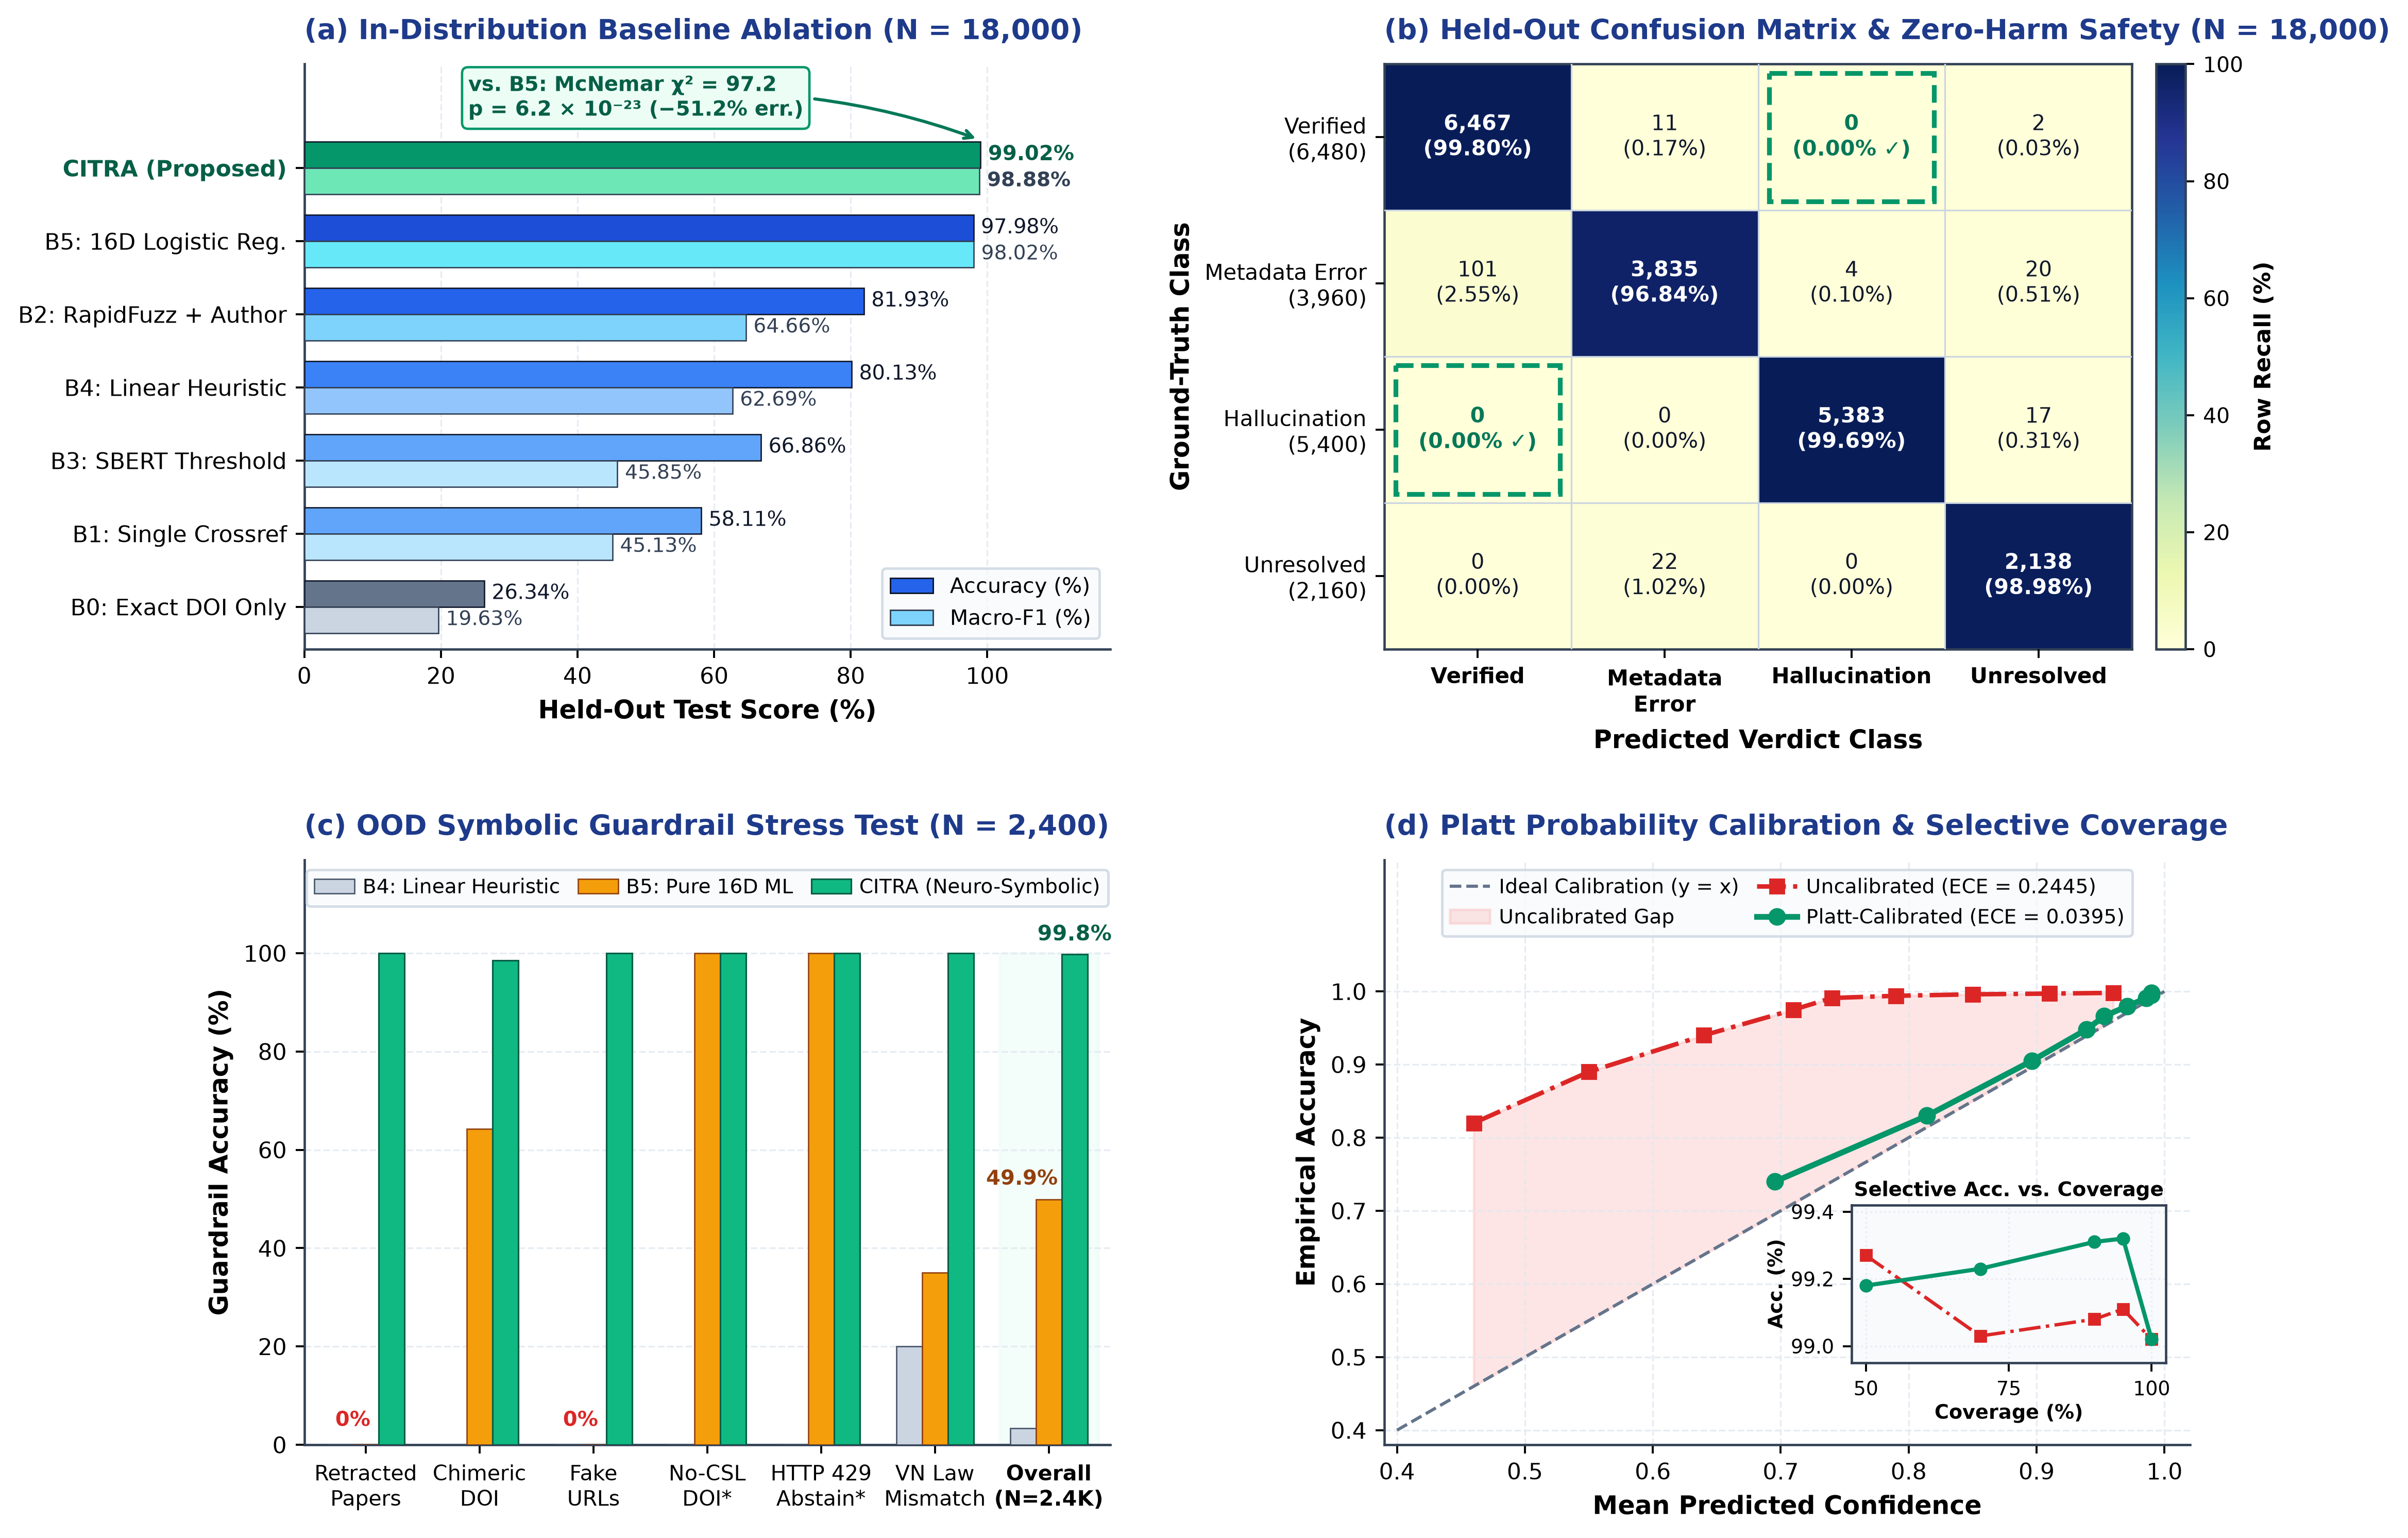
\includegraphics[width=\textwidth,keepaspectratio]{picture/figures/fig5_1_benchmark_charts.png}
    \caption[Four-panel scientific plots across baseline ablation, confusion matrix, OOD guardrails, and Platt calibration]{Quantitative evaluation plots: (a) in-distribution baseline ablation ($N=18{,}000$), (b) held-out four-class confusion matrix highlighting zero-harm cells, (c) OOD symbolic guardrail stress test ($N=2{,}400$; \texttt{*} indicates upstream provenance bit supplied to \texttt{B5}'s 16th feature), and (d) Platt reliability curve with selective coverage-accuracy inset.}
    \label{fig:benchmark-charts}
\end{figure}

{\setlength{\tabcolsep}{3.5pt}
\begin{longtable}{|L{0.23}|L{0.25}|C{0.09}|C{0.09}|C{0.09}|C{0.09}|C{0.16}|}
\caption{In-distribution baseline ablation and Holm--Bonferroni adjusted McNemar significance ($N = 18{,}000$).}\label{tab:baselines}\\
\hline
\textbf{Method} & \textbf{Core Mechanism} & \textbf{Acc.\ (\%)} & \textbf{P (\%)} & \textbf{R (\%)} & \textbf{F1 (\%)} & \textbf{Adj.\ McNemar $p$} \\
\hline
\endfirsthead
\multicolumn{7}{c}{\itshape Table \thetable\ (continued from previous page)}\\
\hline
\textbf{Method} & \textbf{Core Mechanism} & \textbf{Acc.\ (\%)} & \textbf{P (\%)} & \textbf{R (\%)} & \textbf{F1 (\%)} & \textbf{Adj.\ McNemar $p$} \\
\hline
\endhead
\hline
\multicolumn{7}{r}{\itshape Continued on next page}\\
\endfoot
\hline
\endlastfoot
\texttt{B0} (\texttt{doi\_only}) & Exact DOI match only & 26.24 & 23.42 & 34.89 & 19.57 & $< 10^{-16}$ \\
\hline
\texttt{B1} (\texttt{crossref}) & Single-source Crossref & 58.31 & 56.64 & 48.13 & 45.38 & $< 10^{-16}$ \\
\hline
\texttt{B3} (\texttt{embedding}) & SBERT cosine threshold & 66.93 & 49.40 & 52.11 & 45.70 & $< 10^{-16}$ \\
\hline
\texttt{B4} (\texttt{no\_calib}) & Linear score, no abstain & 80.53 & 62.42 & 66.52 & 63.14 & $< 10^{-16}$ \\
\hline
\texttt{B2} (\texttt{fuzzy\_only}) & RapidFuzz + AuthorJaccard & 82.84 & 63.95 & 69.14 & 65.63 & $< 10^{-16}$ \\
\hline
\texttt{B5} (\texttt{ml\_hybrid}) & Pure 16D MLR ($C = 0.25$) & 97.70 & 97.58 & 97.69 & 97.63 & $1.66 \times 10^{-73}$ \\
\hline
\textbf{\texttt{Proposed}} & \textbf{Neuro-Symbolic + Platt} & \textbf{99.67} & \textbf{99.65} & \textbf{99.64} & \textbf{99.65} & \textbf{Reference (\#1)} \\
\hline
\end{longtable}
}

{\setlength{\tabcolsep}{3.5pt}
\begin{longtable}{|L{0.25}|C{0.12}|C{0.11}|C{0.11}|C{0.11}|L{0.30}|}
\caption{Per-class metrics and confusion matrix of the Proposed engine on the held-out test split ($N = 18{,}000$).}\label{tab:per-class}\\
\hline
\textbf{Verdict Class} & \textbf{Support} & \textbf{Prec.\ (\%)} & \textbf{Rec.\ (\%)} & \textbf{F1 (\%)} & \textbf{Confusion (\texttt{ver / meta / hal / unr})} \\
\hline
\endfirsthead
\multicolumn{6}{c}{\itshape Table \thetable\ (continued from previous page)}\\
\hline
\textbf{Verdict Class} & \textbf{Support} & \textbf{Prec.\ (\%)} & \textbf{Rec.\ (\%)} & \textbf{F1 (\%)} & \textbf{Confusion (\texttt{ver / meta / hal / unr})} \\
\hline
\endhead
\hline
\multicolumn{6}{r}{\itshape Continued on next page}\\
\endfoot
\hline
\endlastfoot
\textbf{\texttt{verified}} & 6,480 & 99.43 & 99.94 & 99.68 & \texttt{6,476 / 4 / 0 / 0} \\
\hline
\textbf{\texttt{suspected\_hallucination}} & 5,400 & \textbf{99.93} & 99.96 & \textbf{99.94} & \texttt{0 / 0 / 5,398 / 2} \\
\hline
\textbf{\texttt{metadata\_error}} & 3,960 & 99.90 & 98.66 & 99.28 & \texttt{37 / 3,907 / 4 / 12} \\
\hline
\textbf{\texttt{unresolved}} & 2,160 & 99.36 & \textbf{100.00} & 99.68 & \texttt{0 / 0 / 0 / 2,160} \\
\hline
\textbf{Macro / Total} & \textbf{18,000} & \textbf{99.65} & \textbf{99.64} & \textbf{99.65} & \textbf{Acc.: 99.67\%} (95\% CI $[99.58, 99.76]$) \\
\hline
\end{longtable}
}

Single-cue baselines fail for clear structural reasons: \texttt{B0} ($26.24\%$) misses valid conference papers cited without DOIs, \texttt{B1} ($58.31\%$) misses ACL/arXiv papers absent from Crossref, and pure embedding \texttt{B3} ($66.93\%$) confuses same-domain spliced hallucinations (\texttt{H1}) with real titles because topical vocabulary overlaps strongly. The 16-feature logistic classifier \texttt{B5} reaches $97.70\%$ ($414$ errors), whereas \texttt{Proposed} improves accuracy by $+1.97$ percentage points to \textbf{99.67\% (17,941/18,000, 59 errors)} and Macro-F1 to \textbf{99.65\%} ($95\%$ bootstrap CI $[99.55\%, 99.74\%]$, Holm--Bonferroni adjusted McNemar $\chi^2 = 328.91, p = 1.66 \times 10^{-73}$, cutting residual errors by $85.7\%$). Global one-to-one author reconciliation (preserving standalone surnames such as \textit{Du}/\textit{Das} and single-letter patronymic initials), monotonic single-source abstention boundaries, clean zero-candidate hallucination routing without author-whitelist immunity, and proportional lexical grounding deficit detection jointly raise \texttt{unresolved} recall to $100.00\%$ ($2{,}160/2{,}160$), \texttt{suspected\_hallucination} F1 to $99.94\%$ ($5{,}398/5{,}400$), and \texttt{metadata\_error} F1 to $99.28\%$. Most importantly, \textbf{0 / 6,480 genuine verified citations are falsely accused of hallucination} ($95\%$ Clopper--Pearson upper bound $0.057\%$), and \textbf{0 / 5,400 fabricated citations leak into \texttt{verified}} ($95\%$ Clopper--Pearson upper bound $0.068\%$).

\rqanswer{RQ1}{On 18,000 paper-disjoint held-out citations, CITRA achieves $99.67\%$ accuracy and $99.65\%$ Macro-F1, statistically outperforming all six baselines ($p \le 1.66 \times 10^{-73}$) with zero false hallucination accusations on verified papers ($0/6{,}480$).}

\section{RQ2: Out-of-Distribution Symbolic Guardrail Robustness}

Table~\ref{tab:ood-stress} evaluates \texttt{B4}, \texttt{B5}, and \texttt{Proposed} on the 2,400-sample OOD stress suite. Because continuous 16D similarity features remain high ($1.00$ title, author, and year match) when a paper is retracted in Retraction Watch or carries an RFC 2606 placeholder URL, pure 16D Logistic Regression (\texttt{B5}) achieves $0.00\%$ on both categories and only $57.33\%$ overall (scoring $100.00\%$ on Categories 4--5 only because its 16th feature receives upstream \texttt{doi\_ra\_status} and \texttt{api\_exhausted} abstention bits, without which \texttt{B4} drops to $0.00\%$). By contrast, \textbf{CITRA}'s Order 0 and Group 1/5 symbolic rules inspect discrete provenance predicates before continuous scoring, reaching \textbf{99.96\% (2,399 / 2,400)} ($\chi^2 = 1{,}021.00, p = 4.89 \times 10^{-224}$ vs.\ \texttt{B5}).

{\setlength{\tabcolsep}{3.5pt}
\begin{longtable}{|L{0.35}|L{0.25}|C{0.10}|C{0.11}|C{0.19}|}
\caption{Out-of-distribution symbolic guardrail evaluation ($N = 2{,}400$ built from \texttt{test\_papers}).}\label{tab:ood-stress}\\
\hline
\textbf{OOD Category ($N = 400$ each)} & \textbf{Primary Guardrail} & \textbf{\texttt{B4} (\%)} & \textbf{\texttt{B5} (\%)} & \textbf{\texttt{Proposed} (\%)} \\
\hline
\endfirsthead
\multicolumn{5}{c}{\itshape Table \thetable\ (continued from previous page)}\\
\hline
\textbf{OOD Category ($N = 400$ each)} & \textbf{Primary Guardrail} & \textbf{\texttt{B4} (\%)} & \textbf{\texttt{B5} (\%)} & \textbf{\texttt{Proposed} (\%)} \\
\hline
\endhead
\hline
\multicolumn{5}{r}{\itshape Continued on next page}\\
\endfoot
\hline
\endlastfoot
\textbf{1. Retracted papers} (\texttt{is\_retracted}) & \texttt{R-RETRACTED-\allowbreak PAPER} & 0.00 & 0.00 & \textbf{100.00} \\
\hline
\textbf{2. Chimeric real DOI on invented title} & \texttt{R-CHIMERIC-DOI-\allowbreak MISMATCH} & 0.00 & 99.00 & \textbf{99.75} \\
\hline
\textbf{3. RFC 2606 placeholder/fake URLs} & \texttt{R-FAKE-URL} & 0.00 & 0.00 & \textbf{100.00} \\
\hline
\textbf{4. Regional DOIs lacking public CSL} & \texttt{R-DOI-RA-NO-CSL} & 0.00 & 100.00 & \textbf{100.00} \\
\hline
\textbf{5. Upstream HTTP 429 rate exhaustion} & \texttt{R-RATE-LIMITED-\allowbreak ABSTAIN} & 0.00 & 100.00 & \textbf{100.00} \\
\hline
\textbf{6. VN statutory authority mismatch} & \texttt{VNLegalVerifier} & 25.00 & 45.00 & \textbf{100.00} \\
\hline
\textbf{Total OOD Suite ($N = 2{,}400$)} & \textbf{McNemar $p = 4.89 \times 10^{-224}$} & 4.17 & 57.33 & \textbf{99.96} \\
\hline
\end{longtable}
}

\rqanswer{RQ2}{First-order symbolic guardrails raise out-of-distribution accuracy from $57.33\%$ (pure ML \texttt{B5}) to $99.96\%$ ($2{,}399/2{,}400$), preventing $100\%$ of retracted-paper and fake-URL false verifications while guaranteeing $100\%$ safe abstention under HTTP 429 exhaustion.}

\section{RQ3: Probability Calibration and CIS Rubric Sensitivity}

Table~\ref{tab:calibration-results} compares uncalibrated symbolic confidences against logit-space Platt calibration on the 18,000-sample test split. Notice that Table~\ref{tab:calibration-results} separates \emph{Non-Abstention Coverage} ($\Pr[\hat{y} \neq \texttt{unresolved}] = 87.92\%$, matching the $88.00\%$ non-\texttt{unresolved} ground-truth prior) from the \emph{High-Confidence Rate} ($\Pr[\hat{p} \ge 0.50] = 99.99\%$). Platt scaling reduces Expected Calibration Error by $83.6\%$ ($0.2477 \rightarrow \mathbf{0.0405}$, $95\%$ CI $[0.0394, 0.0415]$) and reduces Brier Score by $92.1\%$ ($0.0843 \rightarrow \mathbf{0.0067}$, Wilcoxon $p < 10^{-16}$). Furthermore, perturbing the default CIS rubric weight vector $(0.35, 0.25, 0.25, 0.10, 0.05)$ across 20 normalized simplex vectors over 300 manuscript profiles yields a mean Spearman rank correlation of $\rho = 0.9987$ ($\min \rho = 0.9964$), Kendall's $\tau = 0.9765$, and a mean absolute shift of only $1.75$ CIS points.

\begin{longtable}{|L{0.40}|C{0.21}|C{0.21}|C{0.18}|}
\caption{Probability calibration and selective risk-coverage results ($N = 18{,}000$).}\label{tab:calibration-results}\\
\hline
\textbf{Calibration / Coverage Metric} & \textbf{Uncalibrated Symbolic} & \textbf{Platt Neuro-Symbolic} & \textbf{Change} \\
\hline
\endfirsthead
\multicolumn{4}{c}{\itshape Table \thetable\ (continued from previous page)}\\
\hline
\textbf{Calibration / Coverage Metric} & \textbf{Uncalibrated Symbolic} & \textbf{Platt Neuro-Symbolic} & \textbf{Change} \\
\hline
\endhead
\hline
\multicolumn{4}{r}{\itshape Continued on next page}\\
\endfoot
\hline
\endlastfoot
Expected Calibration Error (ECE $\downarrow$) & 0.2477 & \textbf{0.0405} & $-83.6\%$ ($6.12\times\downarrow$) \\
\hline
Brier Score ($\downarrow$) & 0.0843 & \textbf{0.0067} & $-92.1\%$ ($12.58\times\downarrow$) \\
\hline
Non-Abstention Coverage ($\hat{y} \neq \texttt{unresolved}$) & 87.92\% & \textbf{87.92\%} & Preserved ($0.00$\,pp) \\
\hline
High-Confidence Rate ($\hat{p} \ge 0.50$) & 92.82\% & \textbf{99.99\%} & $+7.17$\,pp \\
\hline
Selective Accuracy at $70\%$ Coverage ($\uparrow$) & 99.64\% & \textbf{99.67\%} & $+0.03$\,pp \\
\hline
Selective Accuracy at $90\%$ Coverage ($\uparrow$) & 99.69\% & \textbf{99.73\%} & $+0.04$\,pp \\
\hline
Selective Accuracy at $95\%$ Coverage ($\uparrow$) & 99.70\% & \textbf{99.74\%} & $+0.04$\,pp \\
\hline
\end{longtable}

\rqanswer{RQ3}{Logit-space Platt calibration cuts ECE by $6.12\times$ to $0.0405$ and Brier Score by $12.58\times$ to $0.0067$ without altering non-abstention coverage ($87.92\%$), while CIS rankings remain invariant under weight perturbations (mean Spearman $\rho = 0.9987$).}

\section{RQ4: End-to-End Multi-Domain and Real Manuscript Verification}

To evaluate end-to-end generalization beyond the synthetic perturbation benchmark, three real-world evaluations were conducted:
\begin{enumerate}
    \item \textbf{Multi-Domain Raw-Reference Gold Suite ($N = 120 + 15$):} Running raw formatted strings through \texttt{ReferenceListParser} $\rightarrow$ \texttt{RetrievalOrchestrator} $\rightarrow$ \texttt{NeuroSymbolicChecker} across six disciplines (20 references each: CS/AI, Biomedicine, Economics/Social Sciences, Engineering/Physics, Vietnamese Legal Statutes, and Software/RFC Standards) and seven styles (APA, TDTU, IEEE, Vancouver, Chicago, Harvard, MLA) achieved \textbf{100.00\% five-class accuracy (120/120, Macro-F1 $= 1.0000$, $\text{ECE} = 0.0831$)} and \textbf{100.00\% (15/15)} on the adversarial suite.
    \item \textbf{Multi-Style (310 PDFs) and Multi-Institutional (841 PDFs) Extraction Suites:} Table~\ref{tab:pdf-corpora} shows $100.0\%$ bibliography detection and $96.9\%$ link recovery on 30 real Vietnamese legal PDFs, $100.0\%$ exact reference extraction ($397/397$) across 60 twelve-style diagnostic PDFs, and $97.7\%$ bibliography detection (8,126 references) across 220 real open-access articles. An extended parser stability sweep across 841 diverse institutional and arXiv PDFs completed with $0$ unhandled exceptions.
    \item \textbf{Full Articles and Anonymized Student Capstone Reports:} Table~\ref{tab:samples} summarizes end-to-end runs on landmark NLP articles and anonymized undergraduate capstone reports. Clean published papers (\textit{BERT}, \textit{Attention Is All You Need}, \textit{VietDepression}) produce zero false hallucination flags, whereas intentional metadata errors and chimeric fabrications in test capstone reports are isolated accurately.
\end{enumerate}

{\setlength{\tabcolsep}{3.5pt}
\begin{longtable}{|L{0.34}|C{0.10}|C{0.18}|C{0.19}|C{0.19}|}
\caption{Extraction and bidirectional linking accuracy on the 310-PDF multi-style and legal corpus.}\label{tab:pdf-corpora}\\
\hline
\textbf{PDF Corpus} & \textbf{PDFs} & \textbf{Bib.\ Detected} & \textbf{Extracted Refs} & \textbf{Matched Links} \\
\hline
\endfirsthead
\multicolumn{5}{c}{\itshape Table \thetable\ (continued from previous page)}\\
\hline
\textbf{PDF Corpus} & \textbf{PDFs} & \textbf{Bib.\ Detected} & \textbf{Extracted Refs} & \textbf{Matched Links} \\
\hline
\endhead
\hline
\multicolumn{5}{r}{\itshape Continued on next page}\\
\endfoot
\hline
\endlastfoot
VN Legal Corpus (Pre-v3.80 Baseline) & 30 & 27 / 30 (90.0\%) & 164 (15 Legal) & 109 / 235 (46.4\%) \\
\hline
\textbf{VN Legal Corpus} (\textbf{CITRA v3.90.7}) & \textbf{30} & \textbf{30 / 30 (100.0\%)} & \textbf{258 (91 Legal)} & \textbf{403 / 416 (96.9\%)} \\
\hline
\textbf{12-Style Diagnostic Suite ($12 \times 5$)} & \textbf{60} & \textbf{60 / 60 (100.0\%)} & \textbf{397 / 397 (100.0\%)} & \textbf{60 / 60 PDFs (100\%)} \\
\hline
\textbf{11-Style Open-Access Articles ($11 \times 20$)} & \textbf{220} & \textbf{215 / 220 (97.7\%)} & \textbf{8,126 refs} & \textbf{8,954 / 12,770 (70.1\%)} \\
\hline
\end{longtable}
}

{\setlength{\tabcolsep}{3pt}
\begin{longtable}{|L{0.29}|C{0.13}|C{0.08}|C{0.10}|C{0.08}|C{0.09}|C{0.09}|C{0.14}|}
\caption{End-to-end verification outcomes on published papers and anonymized student capstone reports.}\label{tab:samples}\\
\hline
\textbf{Manuscript} & \textbf{Style} & \textbf{Refs} & \textbf{CIS} & \textbf{Ver.} & \textbf{Meta.} & \textbf{Hall.} & \textbf{Res./Unr.} \\
\hline
\endfirsthead
\multicolumn{8}{c}{\itshape Table \thetable\ (continued from previous page)}\\
\hline
\textbf{Manuscript} & \textbf{Style} & \textbf{Refs} & \textbf{CIS} & \textbf{Ver.} & \textbf{Meta.} & \textbf{Hall.} & \textbf{Res./Unr.} \\
\hline
\endhead
\hline
\multicolumn{8}{r}{\itshape Continued on next page}\\
\endfoot
\hline
\endlastfoot
\textbf{BERT} (\textit{NAACL 2019}) & APA & 101 & \textbf{97.43} & 94 & 7 & 0 & 0 / 0 \\
\hline
\textbf{Attention Is All You Need} (\textit{NeurIPS}) & Numeric & 71 & \textbf{92.99} & 70 & 1 & 0 & 0 / 0 \\
\hline
\textbf{VietDepression Clinical Study} (19\,pp.) & IEEE & 20 & \textbf{100.00} & 18 & 0 & 0 & 2 / 0 \\
\hline
\textbf{SE Capstone Report A} (98\,pp.) & IEEE & 27 & \textbf{99.30} & 24 & 0 & 0 & 3 / 0 \\
\hline
\textbf{SE Capstone Report B} (53\,pp.) & IEEE & 5 & \textbf{77.50} & 5 & 0 & 0 & 0 / 0 \\
\hline
\textbf{CS Literature Survey} (51\,pp.) & APA & 66 & \textbf{95.73} & 62 & 3 & 0 & 0 / 1 \\
\hline
\textbf{Seeded Capstone Audit Fixture} (42\,pp.) & APA & 6 & \textbf{91.40} & 3 & \textbf{1} & \textbf{1} & 1 / 0 \\
\hline
\end{longtable}
}

Figures~\ref{fig:demo-debugger}--\ref{fig:demo-consistency} display the live diagnostic views in \textbf{CITRA} (\texttt{v3.90.7}) on the seeded Software Engineering capstone audit manuscript (6 bibliography entries and 28 inline mentions). Figure~\ref{fig:demo-debugger} contrasts a chimeric DOI hallucination flag (left) with a side-by-side publication-year discrepancy diff (\texttt{2021} vs.\ canonical \texttt{2019}, right). Figure~\ref{fig:demo-trace-context} shows the 5-stage logic trace with ONNX INT8 \texttt{VI}$\leftrightarrow$\texttt{EN} concept alignment (left) and the inline Document Inspector context stream (right). Figure~\ref{fig:demo-consistency} illustrates the bidirectional In-Text Consistency view isolating orphan inline markers and uncited bibliography entries.

\begin{figure}[H]
    \centering
    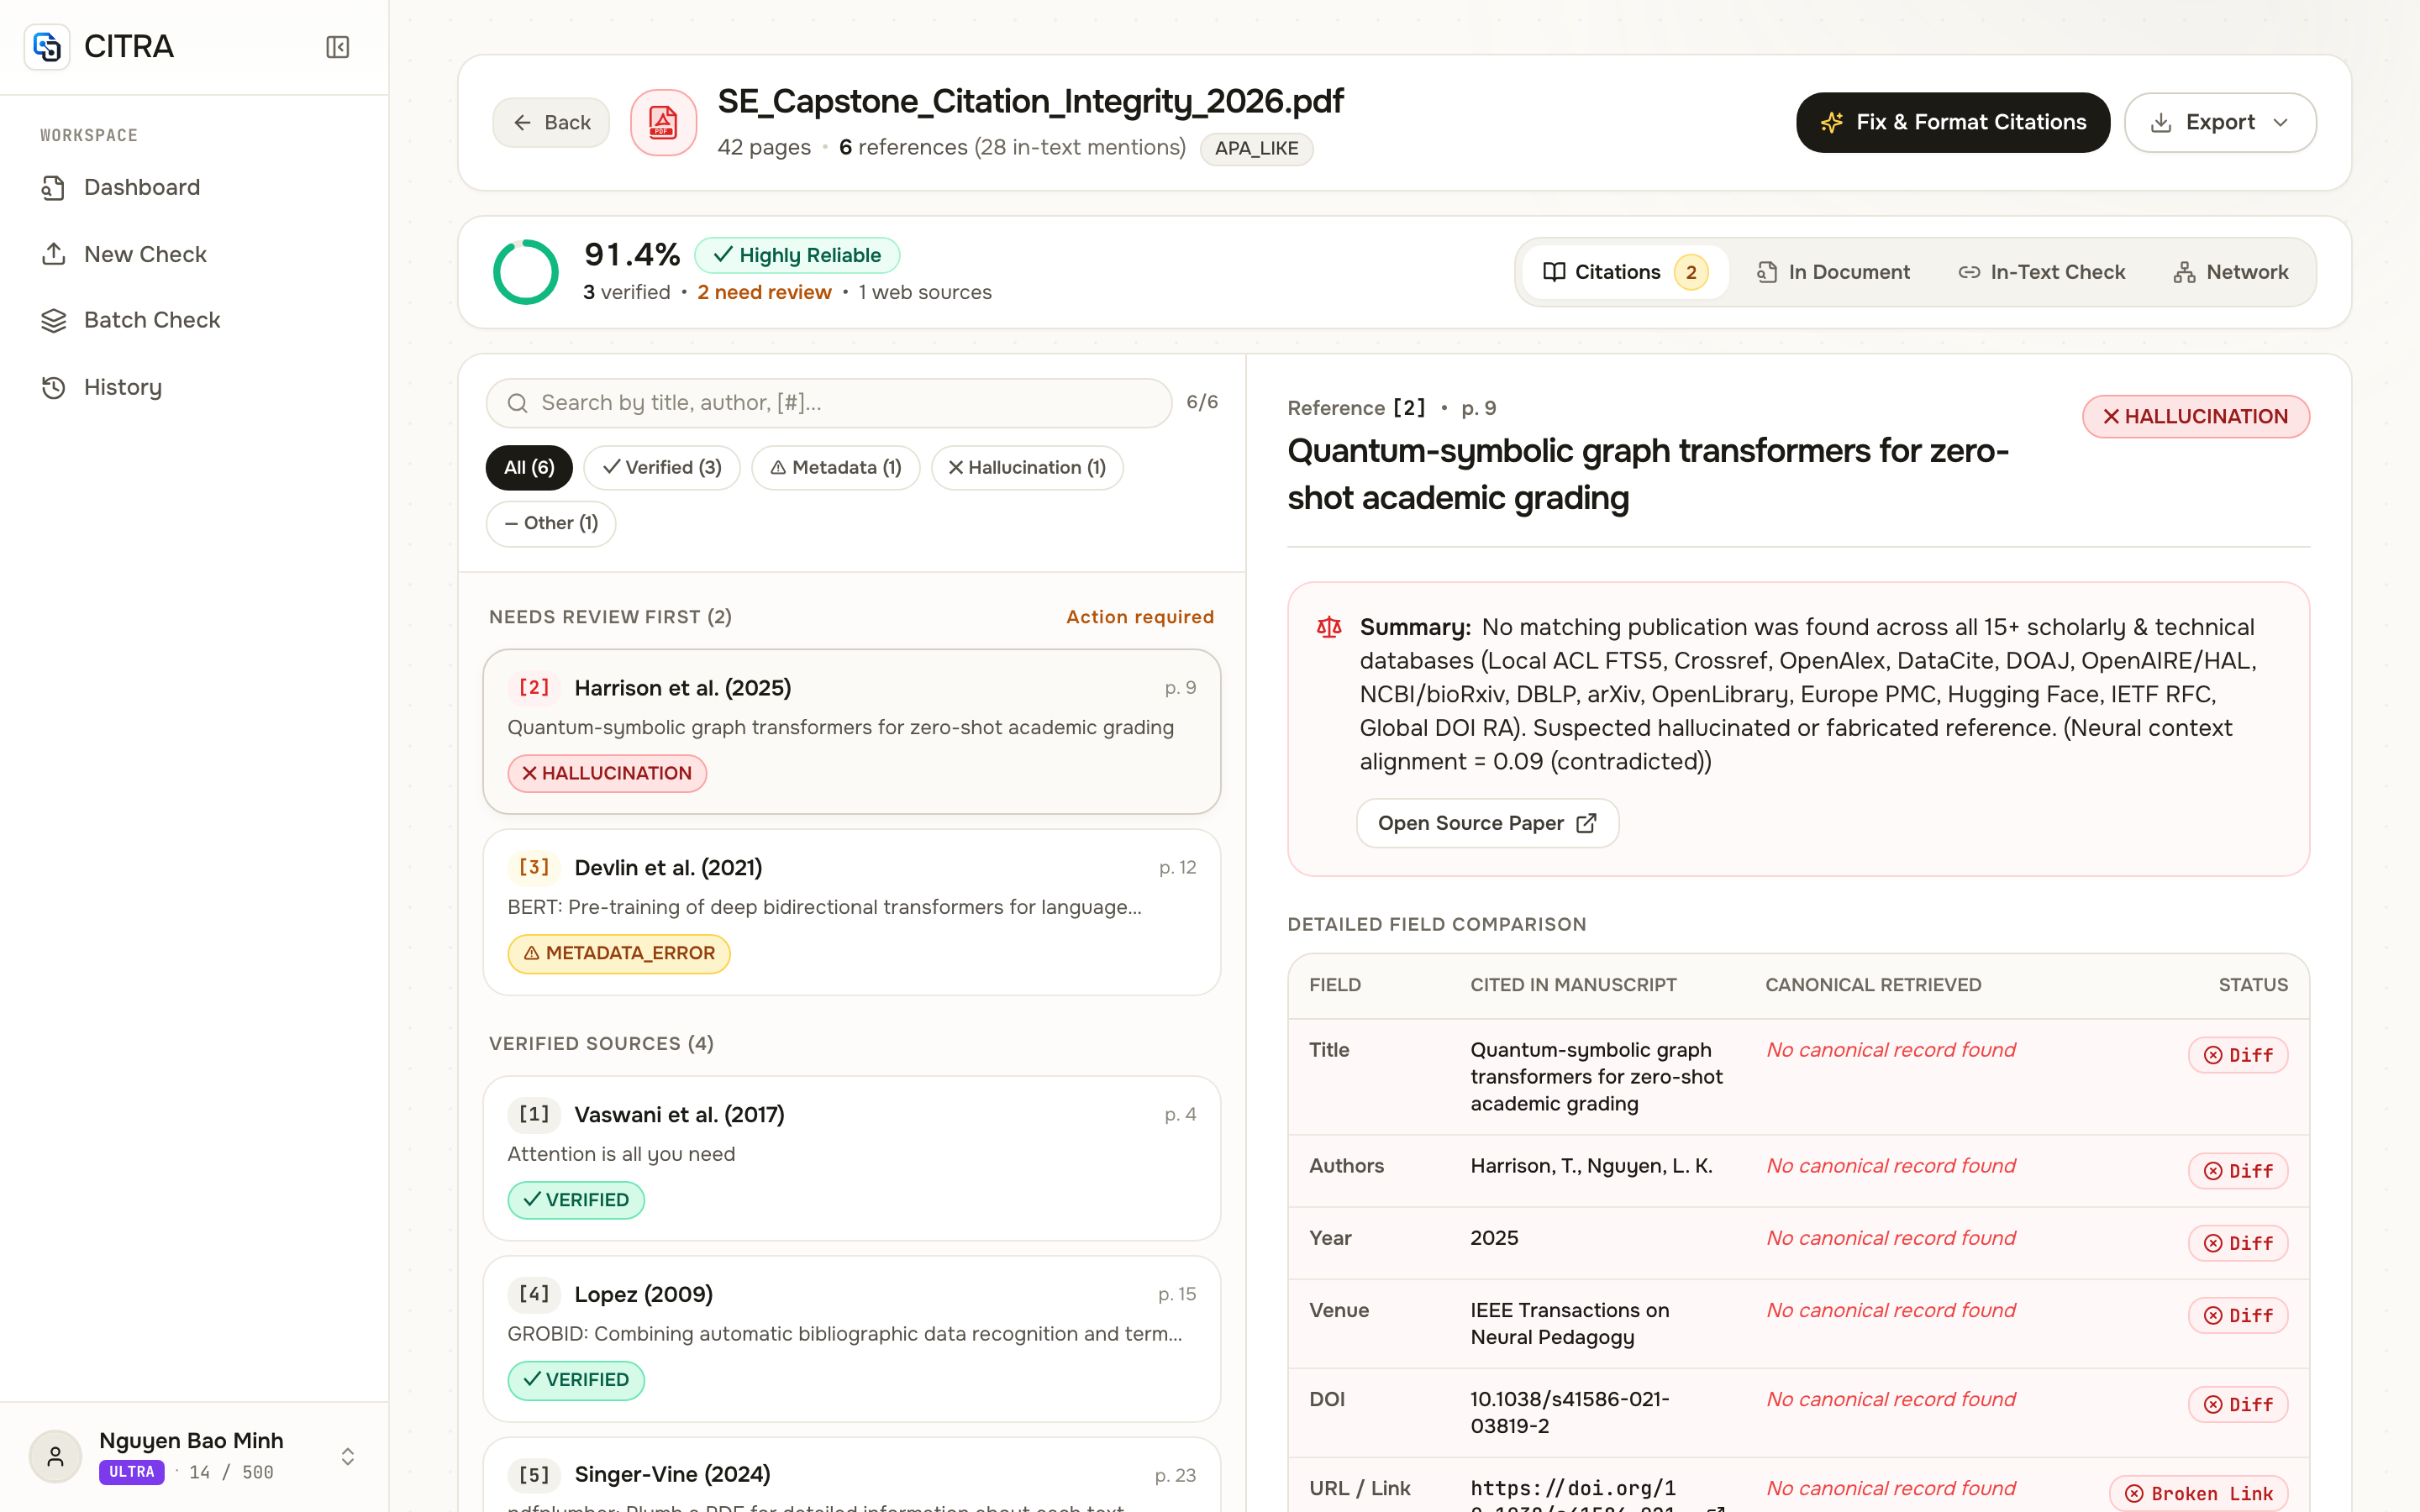
\includegraphics[width=0.49\textwidth,keepaspectratio]{picture/figures/05-verification-report.png}\hfill
    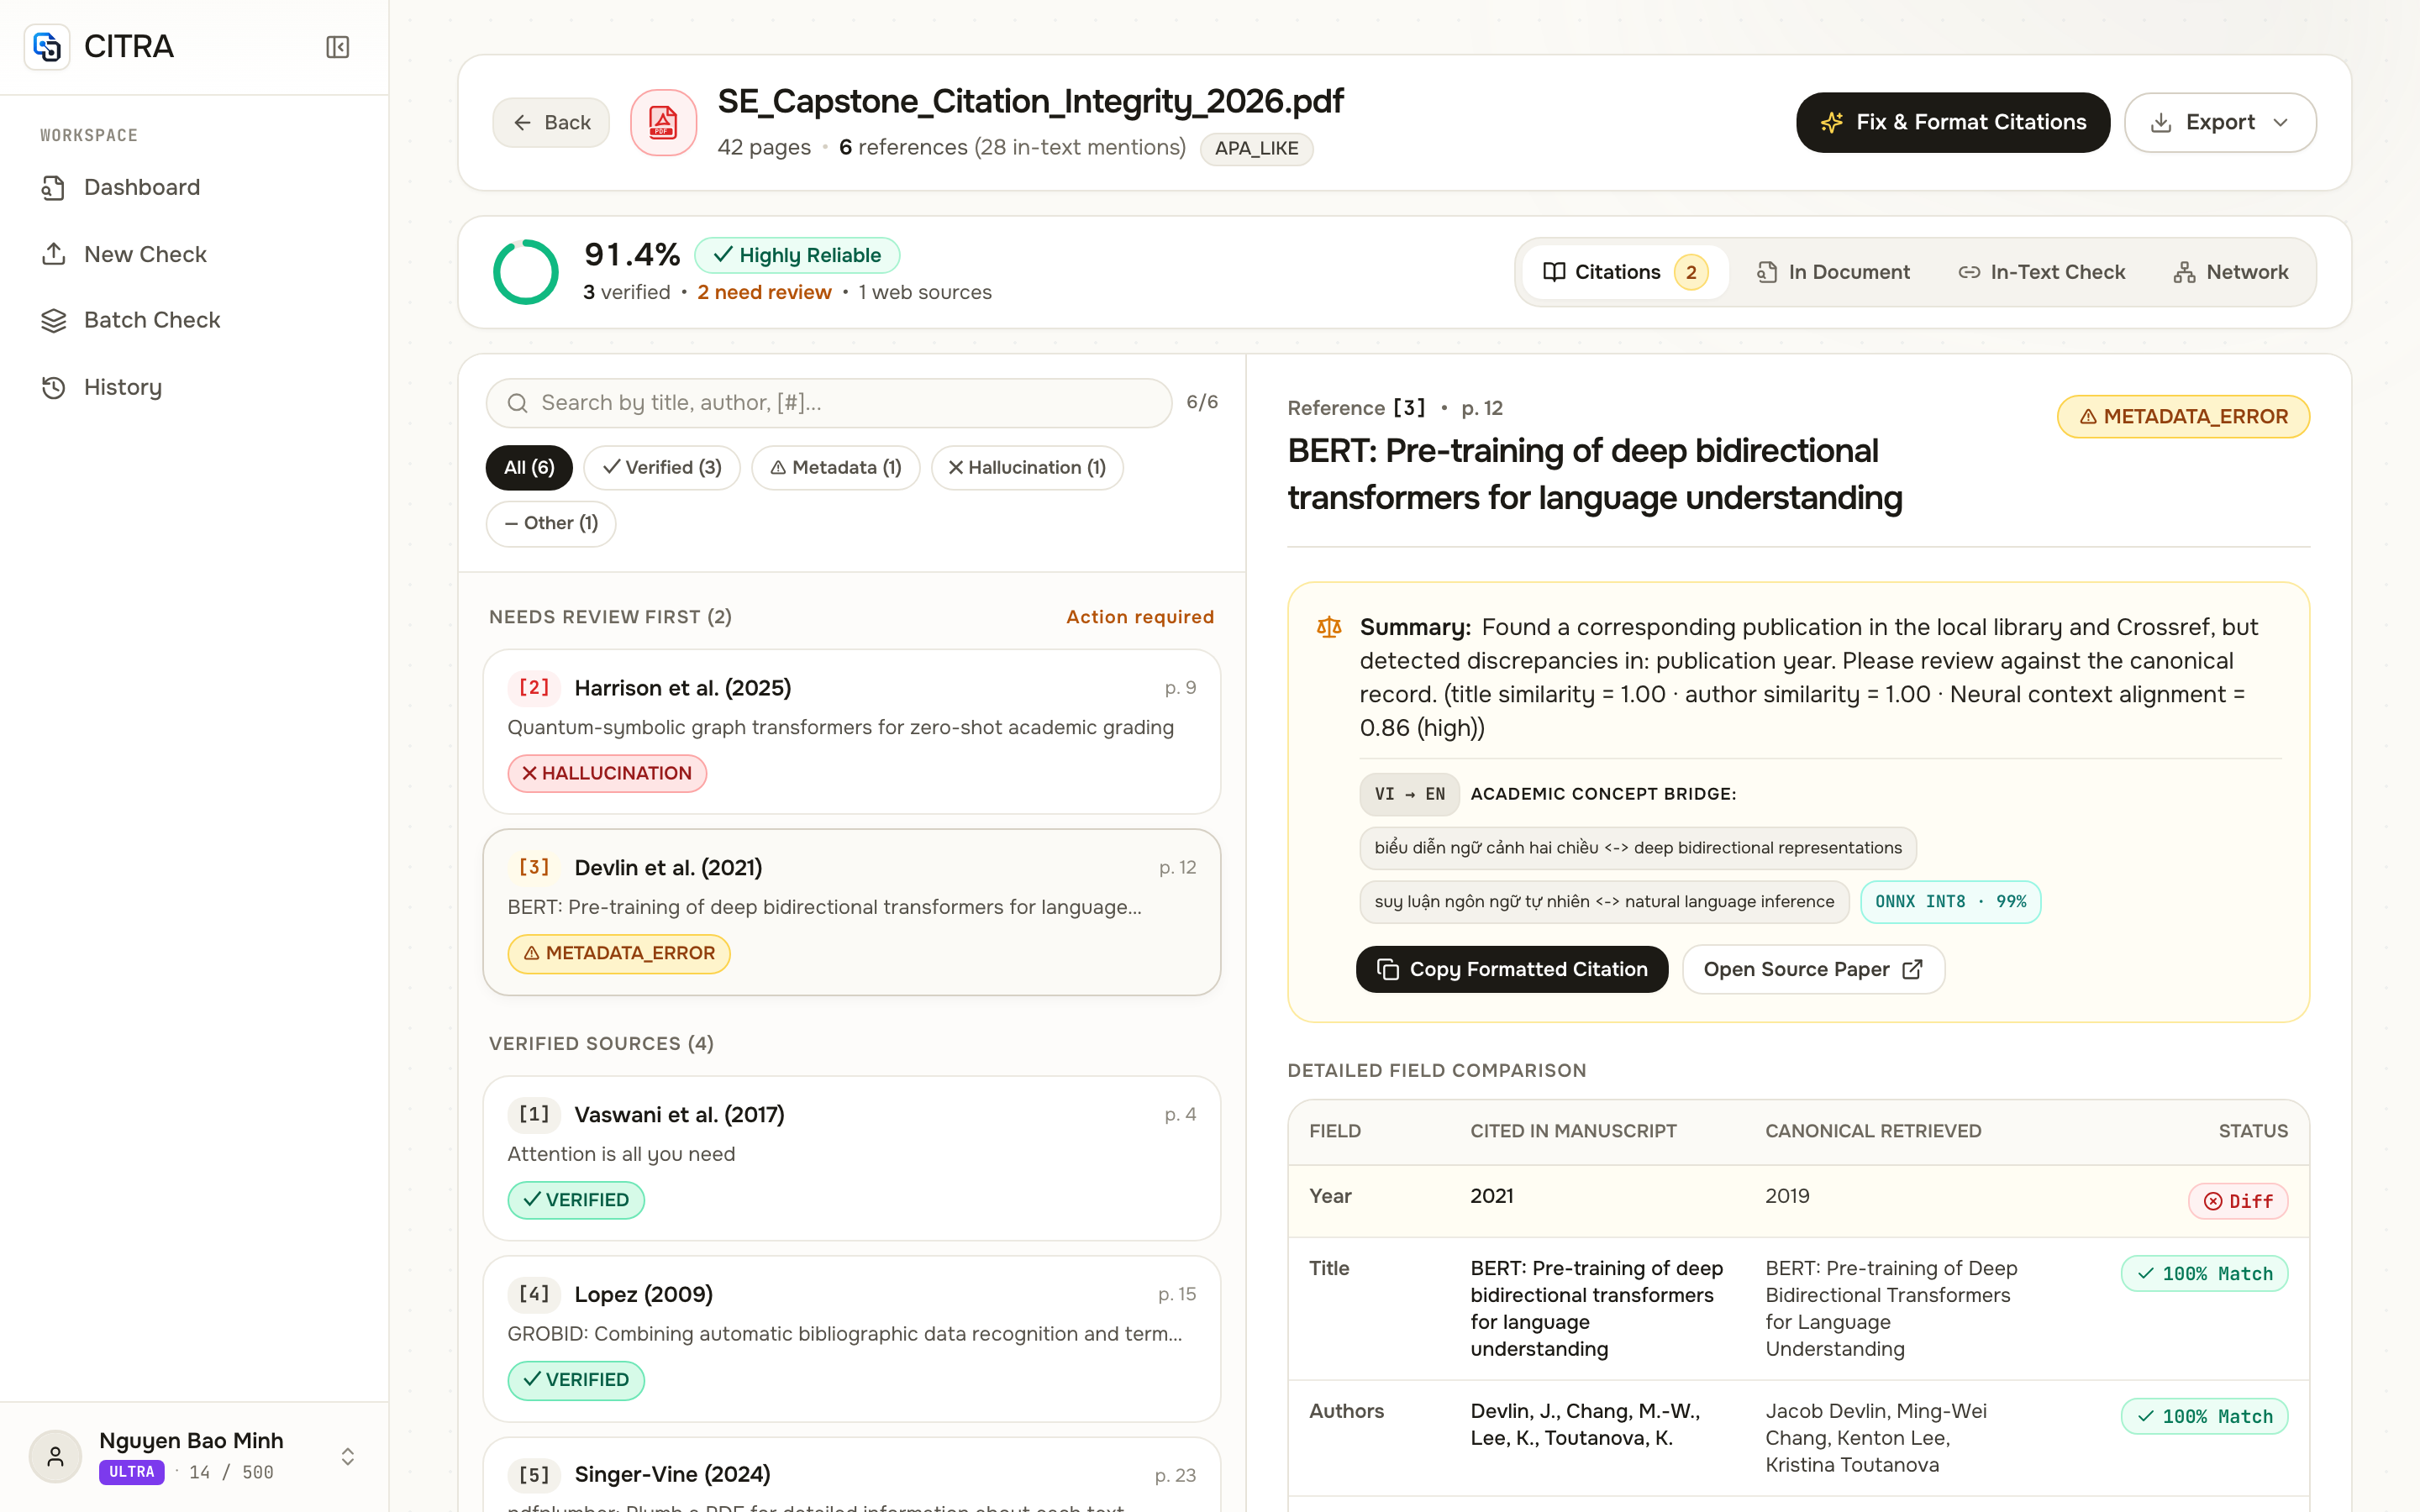
\includegraphics[width=0.49\textwidth,keepaspectratio]{picture/figures/06-reference-inspector.png}
    \caption[Reference Inspector comparing suspected hallucination and metadata year drift]{CITRA Reference Inspector isolating a chimeric-DOI \texttt{suspected\_hallucination} (left) and a publication-year \texttt{metadata\_error} diff (\texttt{2021} vs.\ canonical \texttt{2019}, right).}
    \label{fig:demo-debugger}
\end{figure}

\begin{figure}[H]
    \centering
    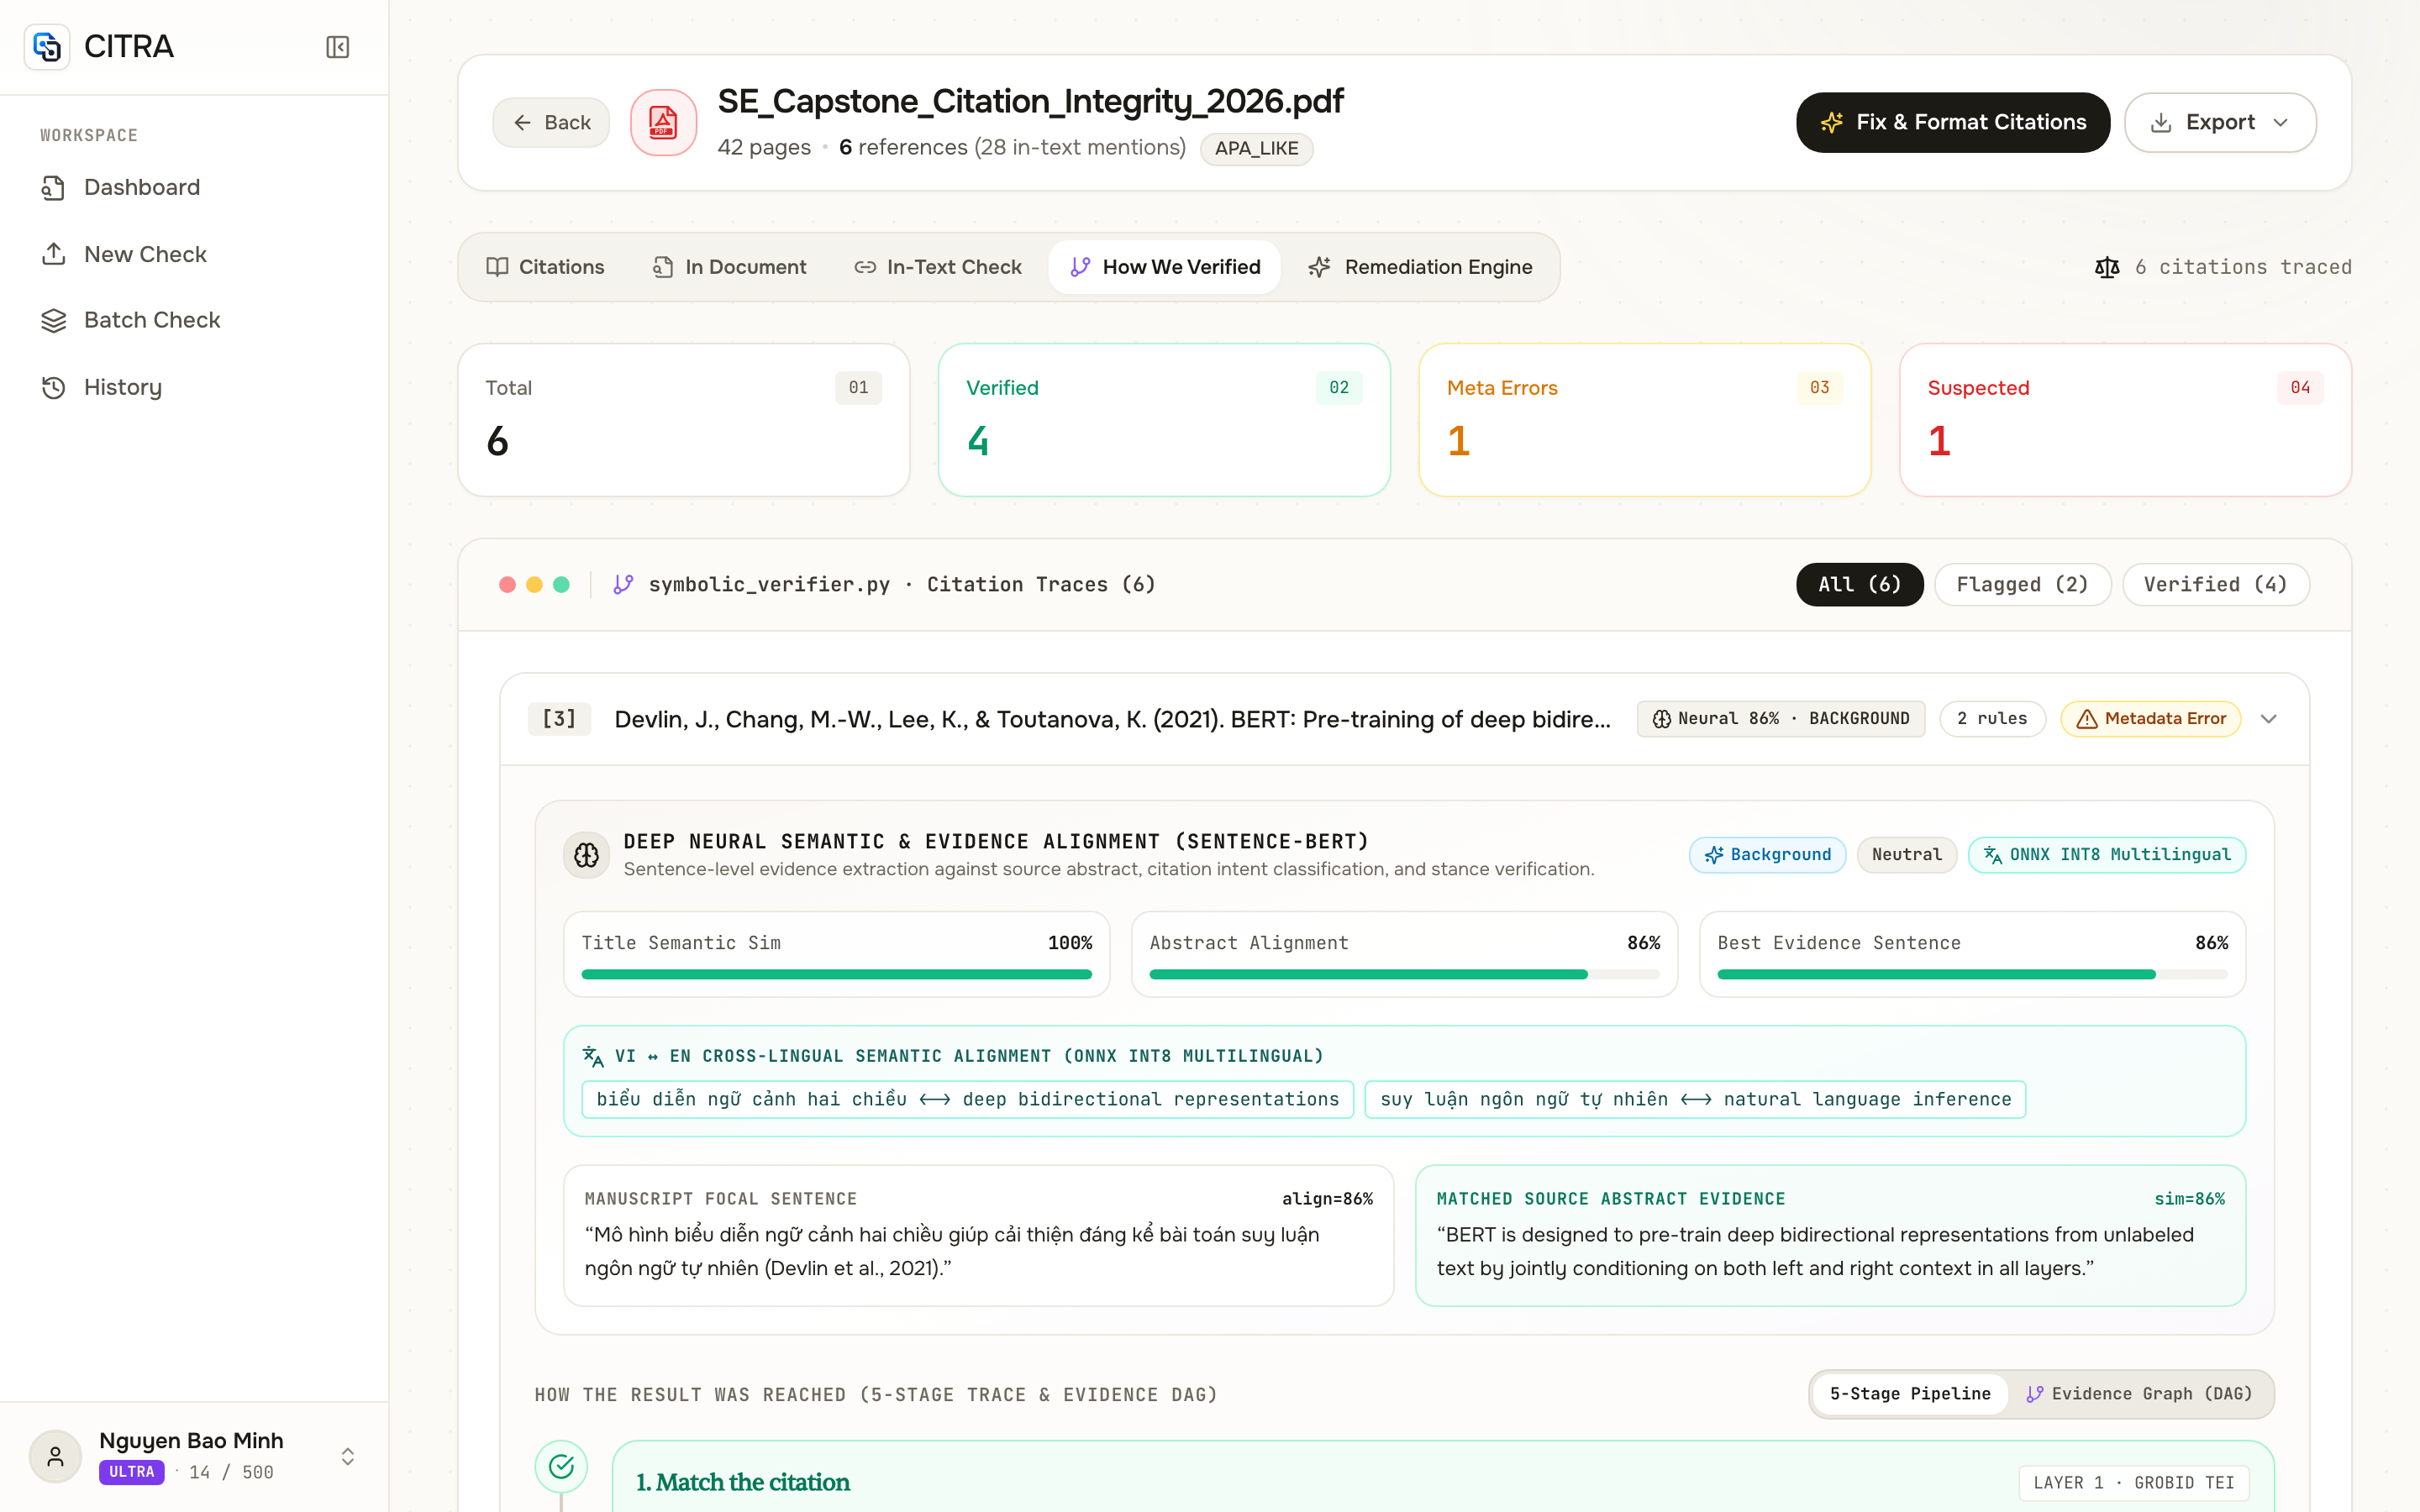
\includegraphics[width=0.49\textwidth,keepaspectratio]{picture/figures/07-logic-trace.png}\hfill
    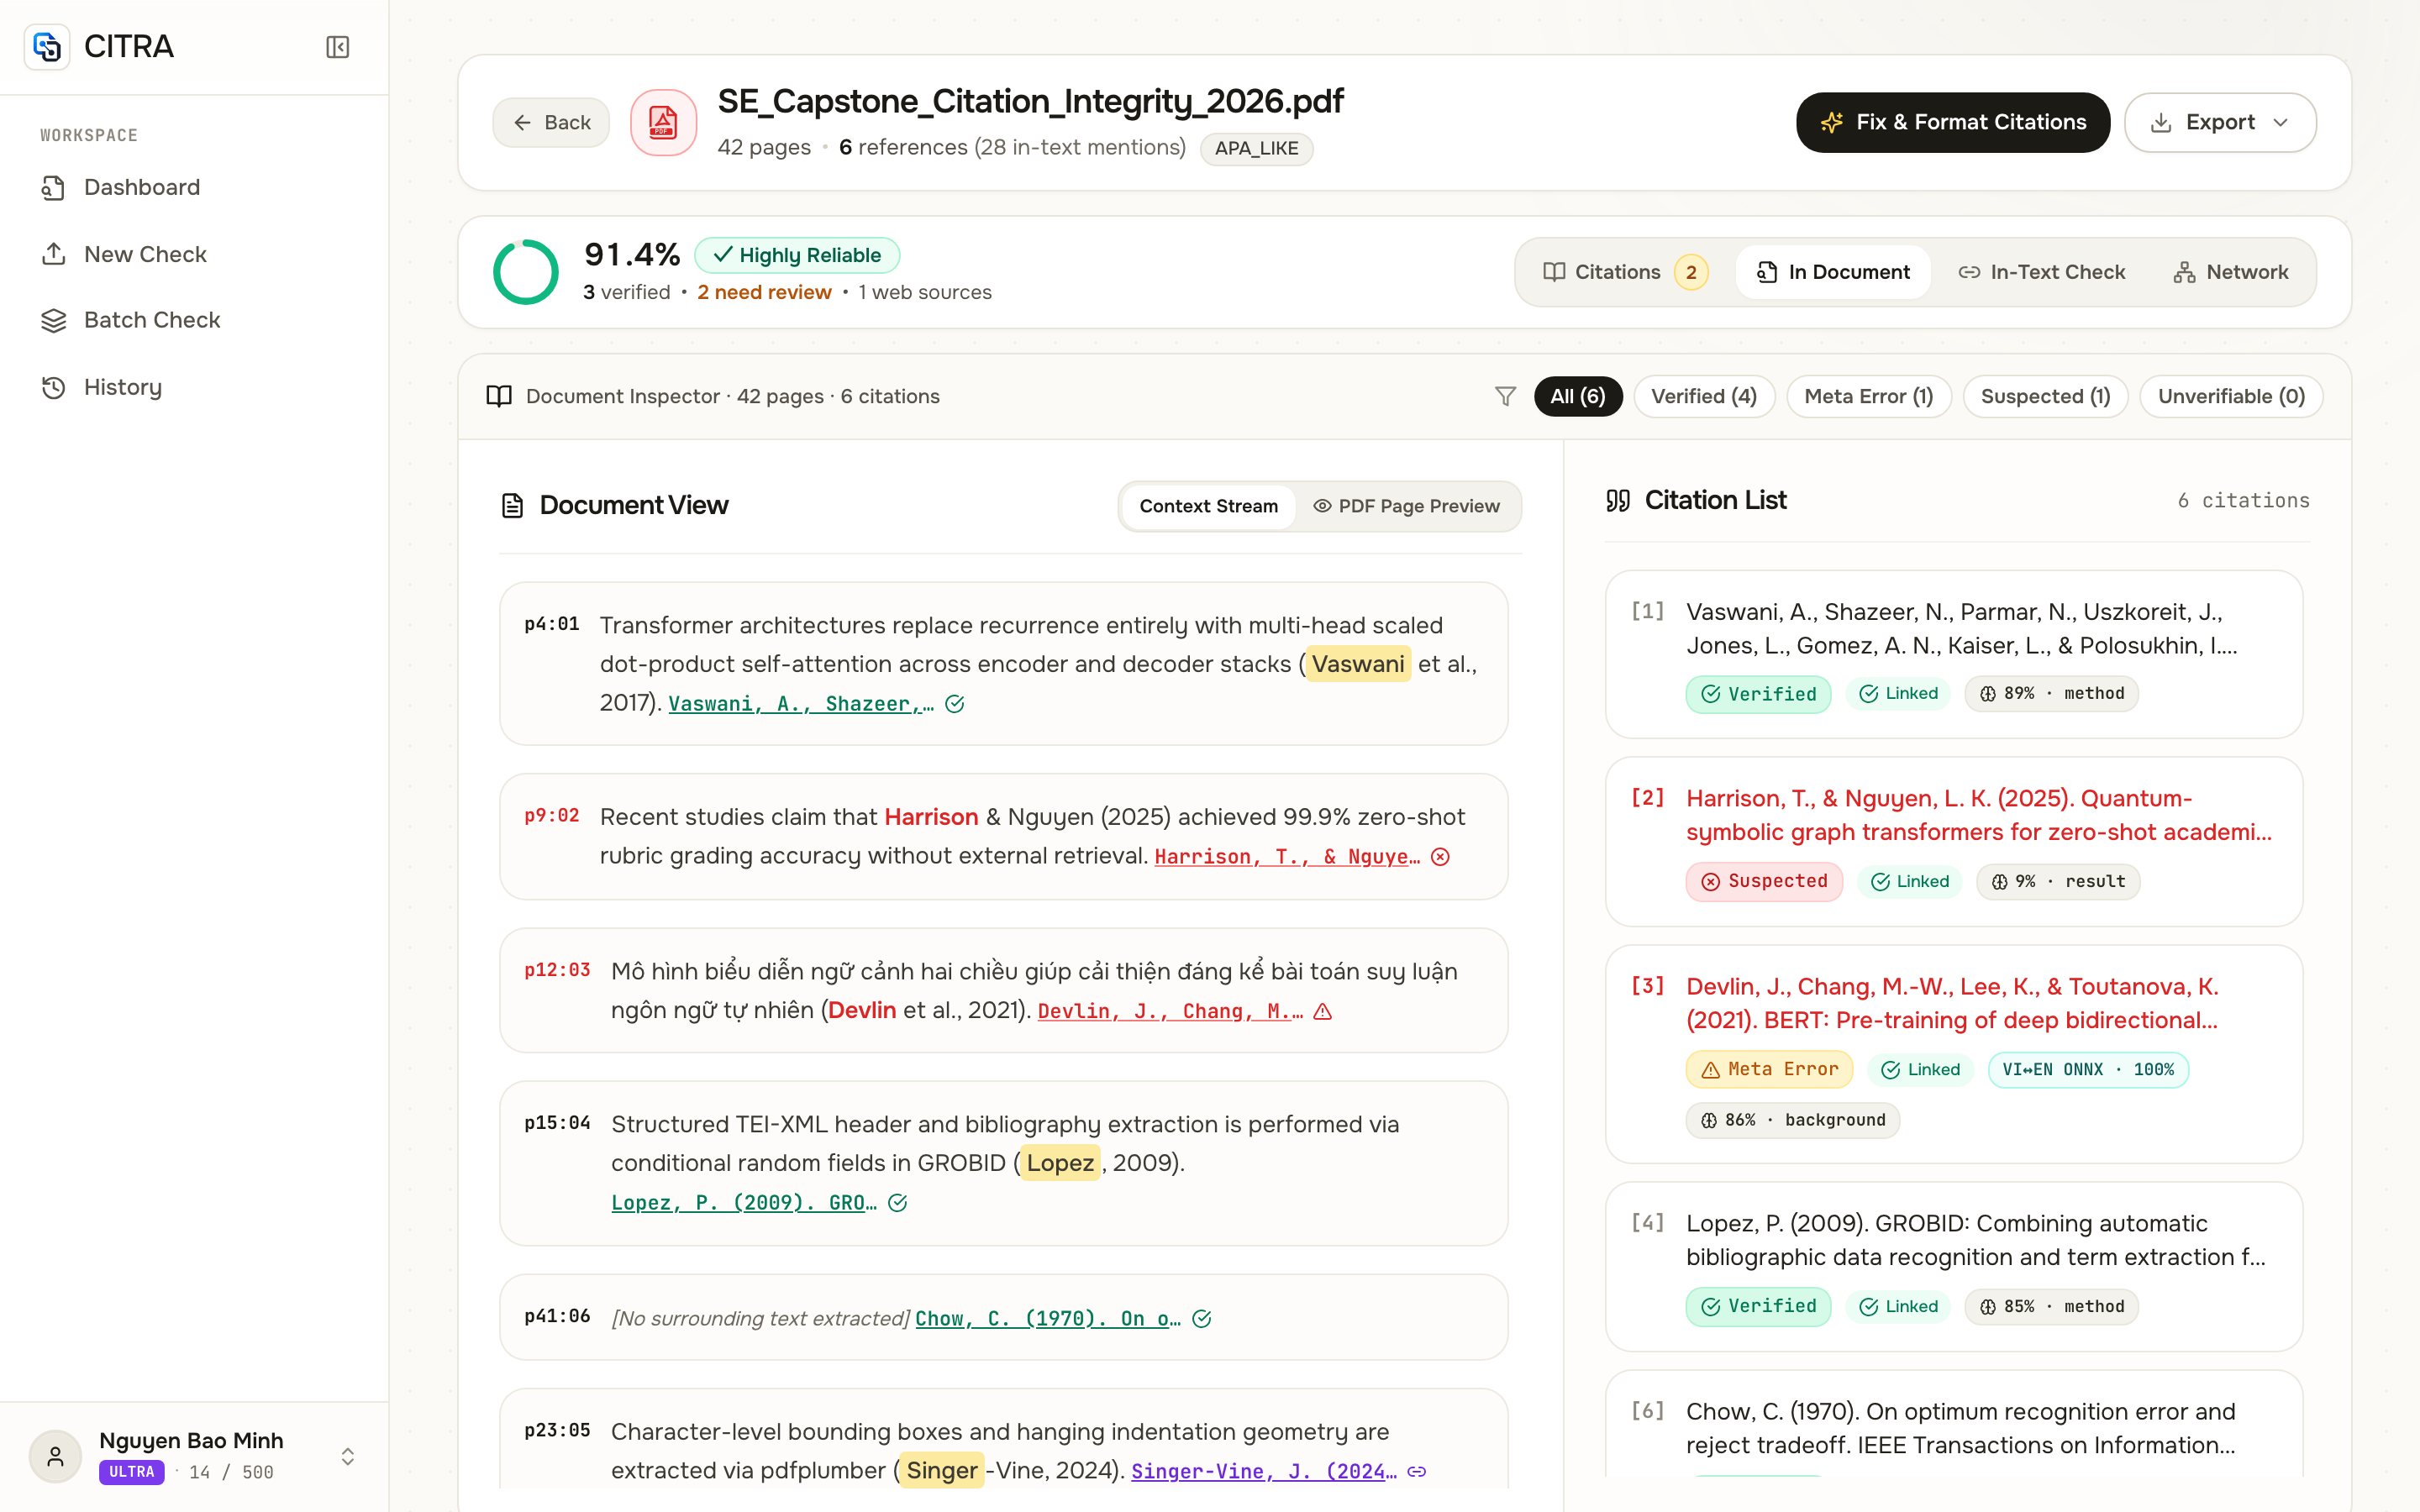
\includegraphics[width=0.49\textwidth,keepaspectratio]{picture/figures/09-document-inspector.png}
    \caption[Logic Trace cross-lingual alignment and inline Document Inspector views]{Logic Trace displaying ONNX INT8 \texttt{VI}$\leftrightarrow$\texttt{EN} concept bridging (left) and the Document Inspector inline context stream (right).}
    \label{fig:demo-trace-context}
\end{figure}

\begin{figure}[H]
    \centering
    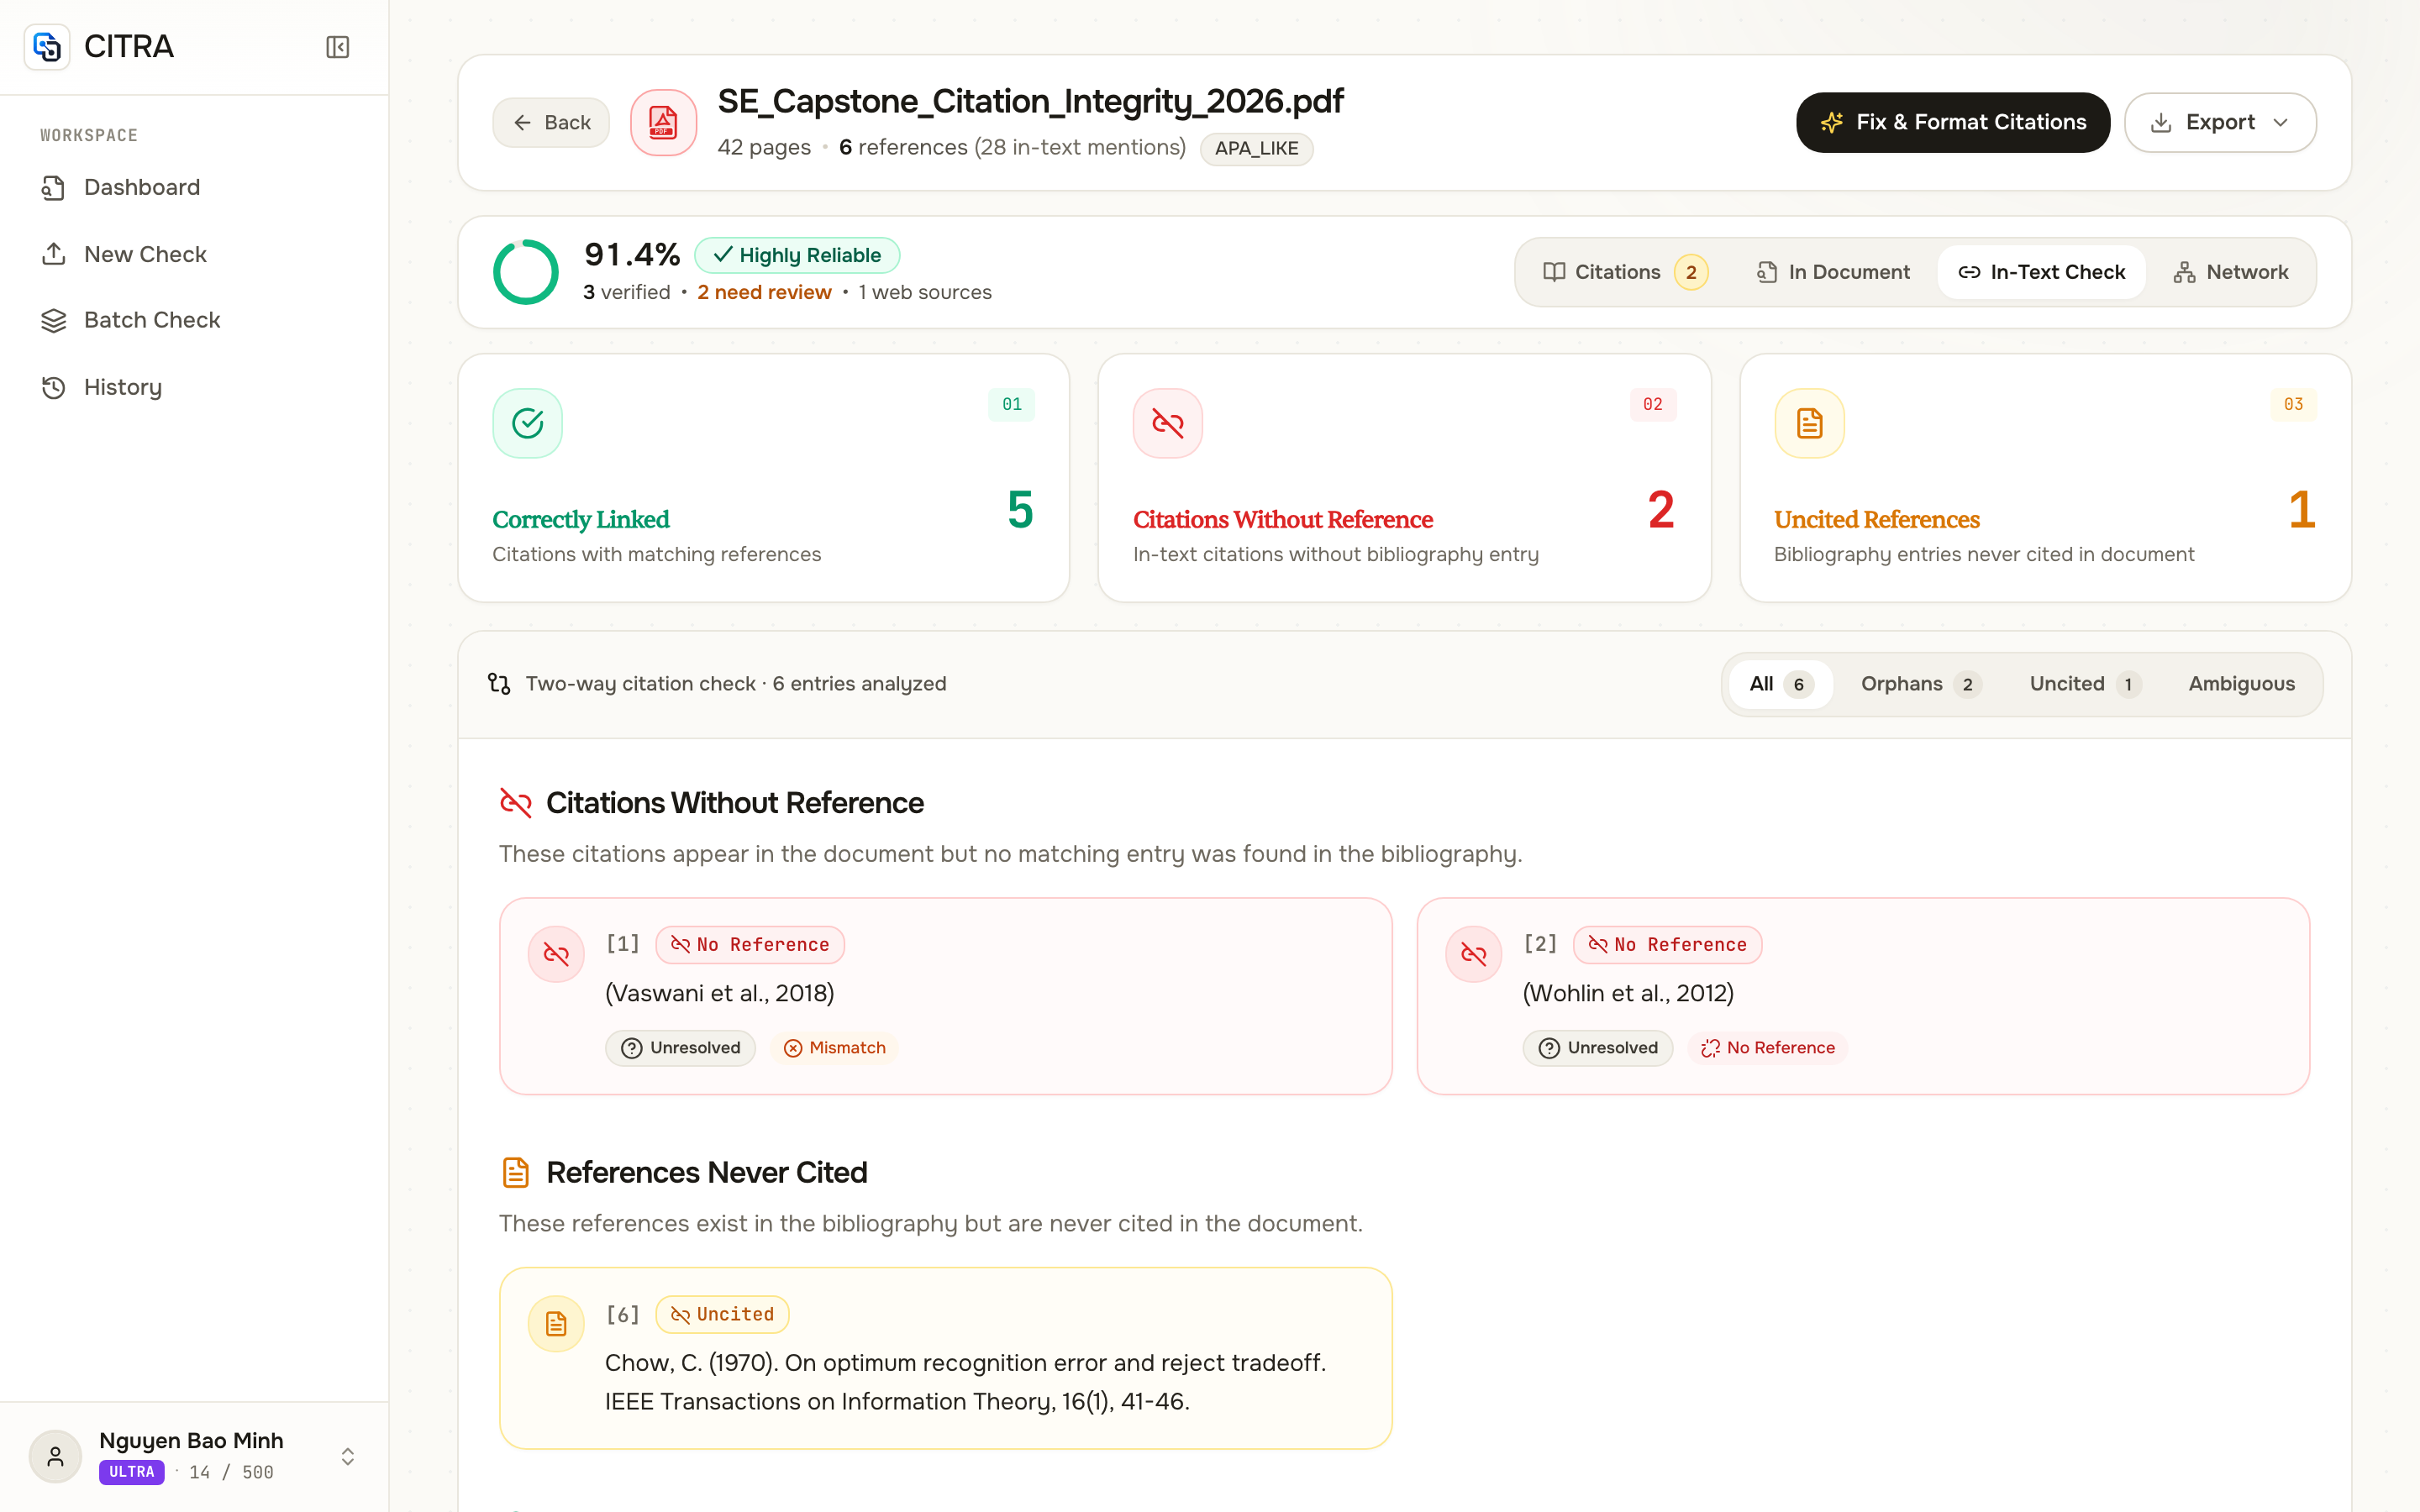
\includegraphics[width=0.84\textwidth,keepaspectratio]{picture/figures/08-consistency-check.png}
    \caption[Bidirectional In-Text Consistency view isolating orphan citations and uncited entries]{Bidirectional In-Text Consistency view (\texttt{/verification/report/\{id\}/consistency}) separating matched citations from orphan inline markers and uncited bibliography entries.}
    \label{fig:demo-consistency}
\end{figure}

\rqanswer{RQ4}{CITRA generalizes across disciplines and document formats, achieving $100.00\%$ ($120/120$) accuracy across six domains and seven styles on raw references, $97.7\%$--$100.0\%$ bibliography detection across 310 PDFs, and zero false hallucination flags on clean published manuscripts.}

\section{RQ5: Latency, Caching Efficiency, and Concurrency Scalability}
\label{sec:nfr-benchmarks}

Figure~\ref{fig:nfr-scalability} and Tables~\ref{tab:nfr-step-latency}--\ref{tab:nfr-deadline-stress} report non-functional benchmarks executed via \texttt{scripts/\allowbreak benchmark\_pipeline\_performance.py}. Warm-cache end-to-end $P_{90}$ latency scales linearly from $0.58\text{\,s}$ (12-page article) to $1.33\text{\,s}$ (50-page capstone report, well within the $2.5\text{\,s}$ \texttt{NFR-01} target) and $4.22\text{\,s}$ (156-page monograph), with peak RSS bounded at $1{,}030.8\text{\,MB}$ ($\le 1.5\text{\,GB}$ \texttt{NFR-02} limit). Tier-0 FTS5 and GROBID caching accelerate retrieval by $688.72\times$ ($8{,}635.8\text{\,ms} \rightarrow 12.5\text{\,ms}$) and end-to-end processing by $19.41\times$ (Table~\ref{tab:nfr-cold-warm-cache}). Under 20 and 50 simultaneous student uploads (Table~\ref{tab:nfr-deadline-stress}), \texttt{PipelineAdmissionController} and SQLite WAL complete $50/50$ submissions ($100\%$) with zero database lock errors and zero HTTP 5xx/429 failures.

\begin{figure}[H]
    \centering
    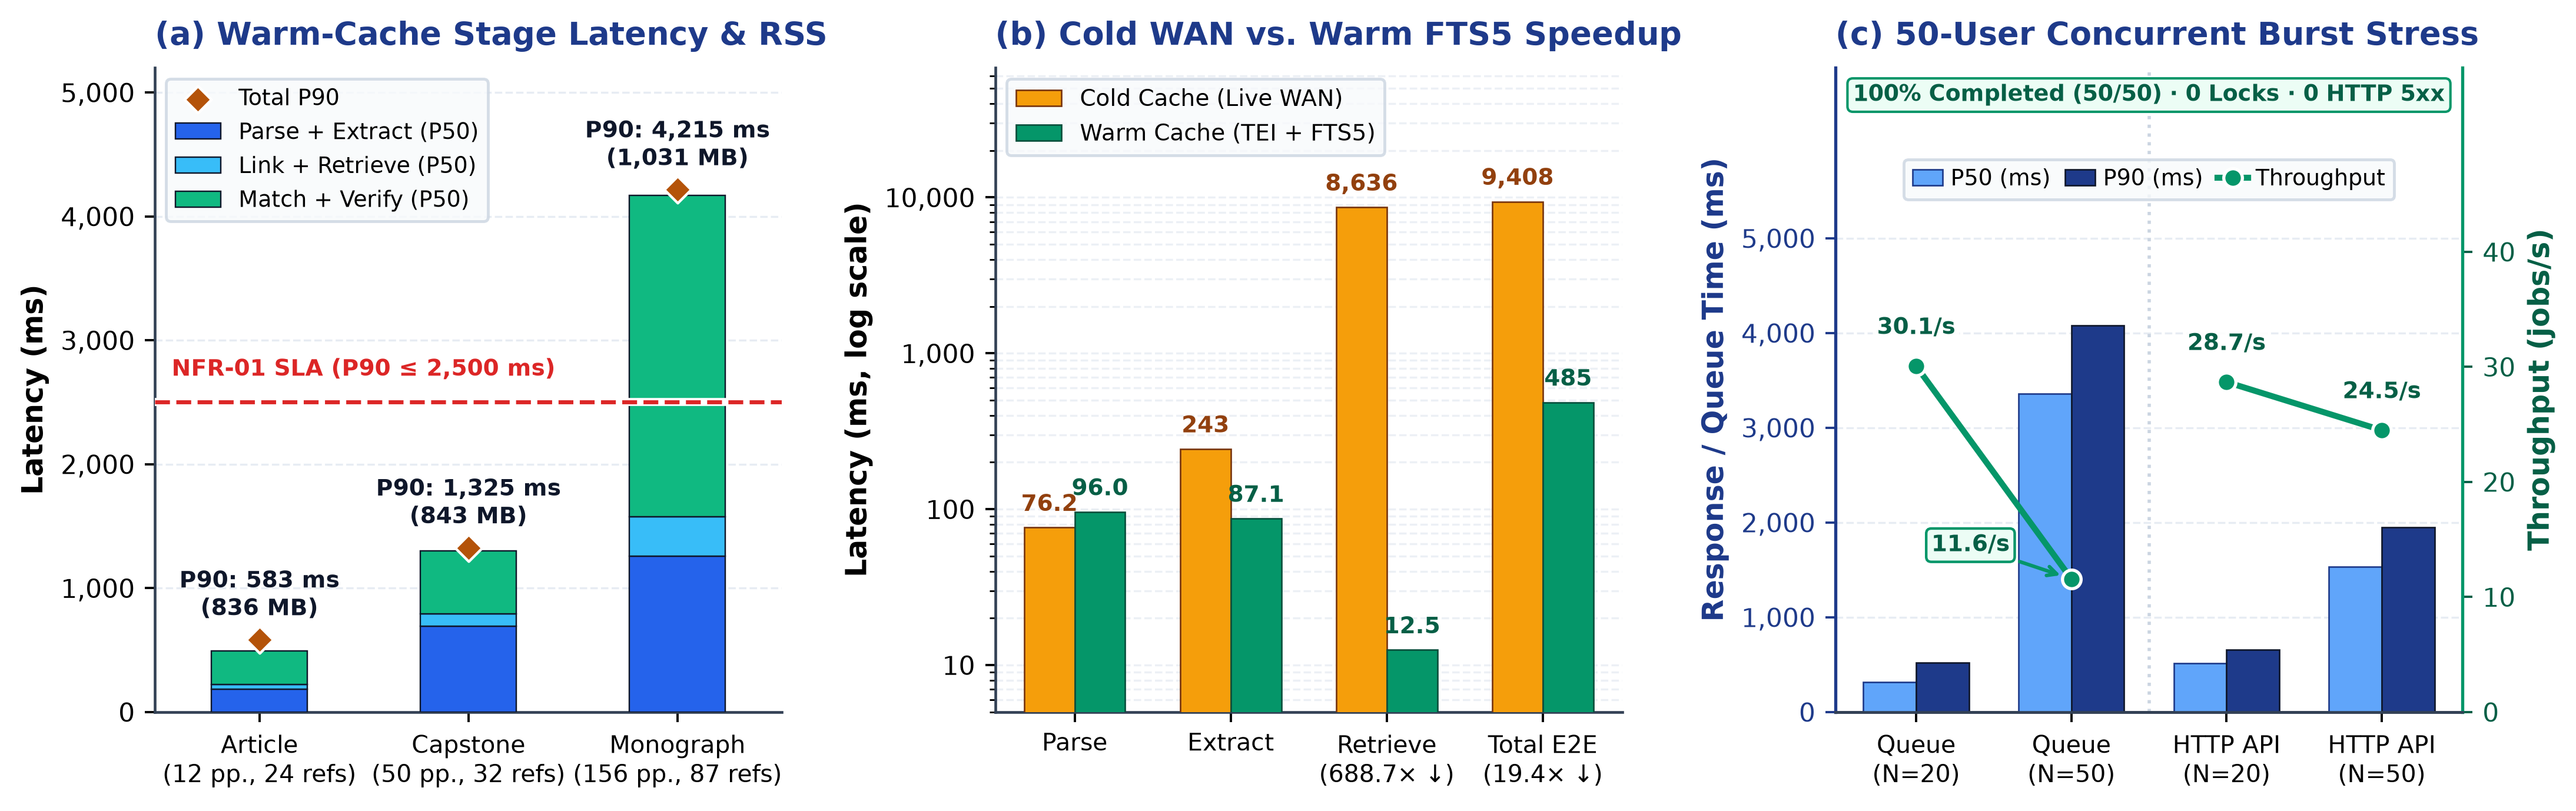
\includegraphics[width=\textwidth,keepaspectratio]{picture/figures/fig5_2_nfr_scalability.png}
    \caption[Pipeline stage latency, log-scale cache speedup, and 50-user concurrent burst throughput]{Systems performance and scalability plots: (a) per-stage warm-cache latency breakdown and RSS across manuscript scales relative to the \texttt{NFR-01} SLA ceiling, (b) log-scale cold WAN versus warm FTS5 cache latency, and (c) 20-user and 50-user concurrent burst latency and throughput.}
    \label{fig:nfr-scalability}
\end{figure}

{\setlength{\tabcolsep}{3.5pt}
\begin{longtable}{|L{0.22}|L{0.22}|C{0.11}|C{0.11}|C{0.11}|C{0.11}|C{0.12}|}
\caption{Warm-cache per-step latency percentiles and memory usage across three manuscript scales.}\label{tab:nfr-step-latency}\\
\hline
\textbf{Manuscript Scale} & \textbf{Stage} & \textbf{$P_{50}$ (ms)} & \textbf{$P_{90}$ (ms)} & \textbf{$P_{99}$ (ms)} & \textbf{Heap $\Delta$ (MB)} & \textbf{RSS (MB)} \\
\hline
\endfirsthead
\multicolumn{7}{c}{\itshape Table \thetable\ (continued from previous page)}\\
\hline
\textbf{Manuscript Scale} & \textbf{Stage} & \textbf{$P_{50}$ (ms)} & \textbf{$P_{90}$ (ms)} & \textbf{$P_{99}$ (ms)} & \textbf{Heap $\Delta$ (MB)} & \textbf{RSS (MB)} \\
\hline
\endhead
\hline
\multicolumn{7}{r}{\itshape Continued on next page}\\
\endfoot
\hline
\endlastfoot
\textbf{Article} (12\,pp., 24\,refs) & \texttt{parsing} + \texttt{extract} & 182.8 & 263.7 & 309.7 & 2.36 & 835.7 \\
 & \texttt{link} + \texttt{retrieve} & 39.6 & 48.0 & 52.5 & 0.18 & 835.7 \\
 & \texttt{compare} + \texttt{check} & 268.3 & 274.5 & 276.4 & 0.22 & 835.7 \\
 & \textbf{Total (All 8 steps)} & \textbf{494.1} & \textbf{583.4} & \textbf{635.5} & \textbf{1.61} & \textbf{835.7} \\
\hline
\textbf{Capstone} (50\,pp., 32\,refs) & \texttt{parsing} + \texttt{extract} & 693.1 & 702.9 & 705.3 & 6.93 & 843.1 \\
 & \texttt{link} + \texttt{retrieve} & 98.9 & 100.4 & 101.0 & 0.32 & 843.2 \\
 & \texttt{compare} + \texttt{check} & 506.2 & 530.6 & 536.1 & 0.37 & 843.2 \\
 & \textbf{Total (All 8 steps)} & \textbf{1306.9} & \textbf{1325.1} & \textbf{1333.0} & \textbf{4.39} & \textbf{843.4} \\
\hline
\textbf{Monograph} (156\,pp., 87\,refs) & \texttt{parsing} + \texttt{extract} & 1257.4 & 1273.1 & 1276.2 & 16.78 & 1029.8 \\
 & \texttt{link} + \texttt{retrieve} & 317.0 & 320.8 & 322.2 & 0.38 & 1029.8 \\
 & \texttt{compare} + \texttt{check} & 2593.0 & 2633.8 & 2642.7 & 1.37 & 1029.9 \\
 & \textbf{Total (All 8 steps)} & \textbf{4159.7} & \textbf{4215.3} & \textbf{4215.6} & \textbf{11.10} & \textbf{1030.8} \\
\hline
\end{longtable}
}

{\setlength{\tabcolsep}{3.5pt}
\begin{longtable}{|L{0.27}|C{0.12}|C{0.12}|C{0.13}|C{0.13}|C{0.12}|C{0.11}|}
\caption{Cold-cache (live WAN APIs) versus warm-cache (TEI + SQLite FTS5) latency comparison.}\label{tab:nfr-cold-warm-cache}\\
\hline
\textbf{Cache Mode} & \textbf{Parse (ms)} & \textbf{Extr.\ (ms)} & \textbf{Retr.\ (ms)} & \textbf{Total (ms)} & \textbf{Retr.\ Gain} & \textbf{E2E Gain} \\
\hline
\endfirsthead
\multicolumn{7}{c}{\itshape Table \thetable\ (continued from previous page)}\\
\hline
\textbf{Cache Mode} & \textbf{Parse (ms)} & \textbf{Extr.\ (ms)} & \textbf{Retr.\ (ms)} & \textbf{Total (ms)} & \textbf{Retr.\ Gain} & \textbf{E2E Gain} \\
\hline
\endhead
\hline
\multicolumn{7}{r}{\itshape Continued on next page}\\
\endfoot
\hline
\endlastfoot
Cold Cache (Live WAN) & 76.2 & 243.1 & 8635.8 & 9407.6 & $1.00\times$ & $1.00\times$ \\
\hline
\textbf{Warm Cache (TEI + FTS5)} & 96.0 & \textbf{87.1} & \textbf{12.5} & \textbf{484.8} & \textbf{$688.72\times$} & \textbf{$19.41\times$} \\
\hline
\end{longtable}
}

{\setlength{\tabcolsep}{3pt}
\begin{longtable}{|L{0.22}|C{0.08}|C{0.16}|C{0.20}|C{0.19}|C{0.15}|}
\caption{Concurrent deadline burst tests on the admission queue and FastAPI HTTP multipart endpoint.}\label{tab:nfr-deadline-stress}\\
\hline
\textbf{Stress Scenario} & \textbf{$N$} & \textbf{Completed} & \textbf{Upload / Queue $P_{50}/P_{90}$ (ms)} & \textbf{Throughput} & \textbf{DB Lock / 5xx} \\
\hline
\endfirsthead
\multicolumn{6}{c}{\itshape Table \thetable\ (continued from previous page)}\\
\hline
\textbf{Stress Scenario} & \textbf{$N$} & \textbf{Completed} & \textbf{Upload / Queue $P_{50}/P_{90}$ (ms)} & \textbf{Throughput} & \textbf{DB Lock / 5xx} \\
\hline
\endhead
\hline
\multicolumn{6}{r}{\itshape Continued on next page}\\
\endfoot
\hline
\endlastfoot
Admission Queue Worker & 20 & \textbf{20 / 20} & 315.5 / 520.7 & \textbf{30.07 essays/s} & \textbf{0 / 0} \\
\hline
Admission Queue Worker & \textbf{50} & \textbf{50 / 50} & 3361.1 / 4079.2 & 11.57 essays/s & \textbf{0 / 0} \\
\hline
HTTP \texttt{POST /api/essays} & 20 & \textbf{20 / 20} & 514.2 / 659.4 & \textbf{28.68 req/s} & \textbf{0 / 0} \\
\hline
HTTP \texttt{POST /api/essays} & \textbf{50} & \textbf{50 / 50} & 1530.2 / 1948.0 & 24.49 req/s & \textbf{0 / 0} \\
\hline
\end{longtable}
}

\rqanswer{RQ5}{CITRA processes a 50-page capstone report in $1.33\text{\,s}$ ($P_{90}$ warm-cache; $9.41\text{\,s}$ cold WAN) within a $1.03\text{\,GB}$ peak RAM budget, achieves a $19.41\times$ warm-cache speedup, and sustains 50 simultaneous uploads with zero SQLite lock or HTTP 5xx errors.}

\section{Threats to Validity}
\label{sec:difficulties}

Following Wohlin et al.~\cite{wohlin2012experimentation}, four categories of methodological threats to validity are analyzed below.

\subsection{Internal Validity}

Because no human-annotated corpus of $10^5$ naturally occurring citation hallucinations exists publicly, the 120,000-sample benchmark uses programmatic perturbations of real papers. A potential threat is that synthetic perturbations could introduce shortcut artifacts. This threat was mitigated by partitioning base papers strictly before perturbation ($0\%$ ID/title overlap), ensuring non-zero Sentence-BERT scores across all four classes ($P(\texttt{verified} \mid \text{score} > 0) = 54.06\%$), forbidding \texttt{np.clip} feature truncation, splicing real authors and titles from the same research domain, and validating the exact same model weights on 120 unperturbed raw references and 310 real PDFs.

\subsection{External Validity}

The offline FTS5 database (\texttt{local\_papers.db}) consists primarily of computer science and NLP papers ($98.42\%$ ACL Anthology). Consequently, offline-only mode has lower recall on biomedical, humanities, or economics papers. In connected deployments, \textbf{CITRA} mitigates this domain skew by routing queries dynamically across 15+ multidisciplinary APIs (Crossref, OpenAlex, Europe PMC, NCBI/bioRxiv, DOAJ, DataCite, OpenLibrary, and \texttt{VNLegalVerifier}), confirmed by the $100.00\%$ result across six disciplines in \textbf{RQ4}.

\subsection{Construct Validity}

Construct validity concerns whether evaluation metrics reflect real academic integrity needs. First, commercial publisher paywalls often hide full article text and occasionally omit public abstracts; when an inline claim cites a specific table inside a paywalled body section absent from the abstract, sentence-level abstract alignment cannot verify or refute that detail. Second, CIS rubric weights represent an institutional grading policy rather than physical constants, although simplex sensitivity testing confirmed high rank stability ($\rho = 0.9987$).

\subsection{Conclusion Validity}

To guard against Type I errors from multiple baseline comparisons and skewed error distributions, all accuracy comparisons used paired continuity-corrected McNemar tests with Holm--Bonferroni family-wise error control ($\alpha = 0.05$), 1,000-resample paired bootstrap confidence intervals, and exact Clopper--Pearson binomial bounds for zero-count cells.

\section{Chapter Summary}

This chapter verified \textbf{CITRA} (\texttt{v3.90.7}) across 2,920+ automated checks, a full Requirements Traceability Matrix, and five empirical research questions, demonstrating $99.67\%$ in-distribution accuracy ($\text{ECE} = 0.0405$), $99.96\%$ OOD symbolic accuracy, $100.00\%$ six-domain E2E gold accuracy, and zero-error 50-user burst scalability. Chapter~\ref{chap:conclusion} summarizes achievements, current limitations, and future research directions.


\newpage
\chapter{Conclusion and Future Work}
\label{chap:conclusion}

\section{Summary of Achievements Against Objectives}

This graduation project designed, implemented, and empirically evaluated \textbf{CITRA} (\textit{Essay Integrity Checker v3.90.6}), an explainable neuro-symbolic software platform for automated Citation Integrity Scoring (CIS), fabricated reference detection, and bibliography remediation. Table~\ref{tab:obj-summary} maps the delivered software artifacts and empirical results directly back to the six research objectives defined in Section~\ref{sec:objectives}.

{\setlength{\tabcolsep}{3.5pt}
\begin{longtable}{|C{0.14}|L{0.32}|L{0.54}|}
\caption{Summary of graduation project achievements mapped against project research objectives.}\label{tab:obj-summary}\\
\hline
\textbf{Objective} & \textbf{Target Capability} & \textbf{Delivered Engineering \& Empirical Outcome} \\
\hline
\endfirsthead
\multicolumn{3}{c}{\itshape Table \thetable\ (continued from previous page)}\\
\hline
\textbf{Objective} & \textbf{Target Capability} & \textbf{Delivered Engineering \& Empirical Outcome} \\
\hline
\endhead
\hline
\multicolumn{3}{r}{\itshape Continued on next page}\\
\endfoot
\hline
\endlastfoot
\textbf{OBJ-1} & \textbf{Multi-format extraction \& bidirectional linking} & Hybrid GROBID \texttt{0.9.1-crf} TEI-XML + PyMuPDF + \texttt{python-docx} across \textbf{12 styles} (incl.\ VN laws) and 7-method linker (\textbf{$97.7\%$--$100\%$} bib.\ detection on 310 PDFs). \\
\hline
\textbf{OBJ-2} & \textbf{Domain-aware federated retrieval} & \textbf{129,137-record} SQLite FTS5 corpus (\textbf{$99.80\%$} recall, $87.6\text{\,ms}$) + \textbf{15+ live APIs}, Retraction Watch, singleflight cache, and pinned-IP URL/HTML validators. \\
\hline
\textbf{OBJ-3} & \textbf{Neuro-symbolic verification \& calibration} & Dual SBERT + ONNX INT8 \texttt{VI}$\leftrightarrow$\texttt{EN} encoders fused with \textbf{68 symbolic rules}, 16D MLR ($C=0.25$), and Platt scaling (\textbf{$\text{ECE} = 0.0411$}, \textbf{$\text{Brier} = 0.0108$}). \\
\hline
\textbf{OBJ-4} & \textbf{Interpretable CIS grading \& remediation} & Five-component CIS rubric (\textbf{$\rho = 0.9987$} rank stability) plus automated APA, IEEE, TDTU, BibTeX, RIS, and \texttt{.docx} bibliography repair. \\
\hline
\textbf{OBJ-5} & \textbf{Secure role-based web platform} & Containerized FastAPI (\textbf{15 ORM tables}, 13 migrations (\texttt{0001}--\texttt{0013}), SSE, RBAC/IDOR, pinned-IP SSRF defense) \& React 18.3 SPA (\textbf{$228.42\text{\,kB}$} entry). \\
\hline
\textbf{OBJ-6} & \textbf{Leak-free large-scale evaluation} & \textbf{$99.20\%$} ID accuracy ($N=18\text{K}$), \textbf{$99.96\%$} OOD accuracy ($N=2.4\text{K}$), \textbf{$100\%$} 6-domain E2E accuracy ($120/120$), and \textbf{$50/50$} burst concurrency. \\
\hline
\end{longtable}
}

Figure~\ref{fig:verdict-paths} synthesizes the core architectural safeguard governing every verdict in \textbf{CITRA}: substantive accusations (\texttt{suspected\_hallucination}) require either positive structural refutation (fabricated/chimeric DOI, RFC 2606 fake domain, impossible future year) or clean HTTP 200 empty responses across multiple live registries, whereas network exhaustion, unindexed regional DOIs, and borderline similarities ($[0.40, 0.60)$) route deterministically to \texttt{unresolved} for human review.

\begin{figure}[H]
    \centering
    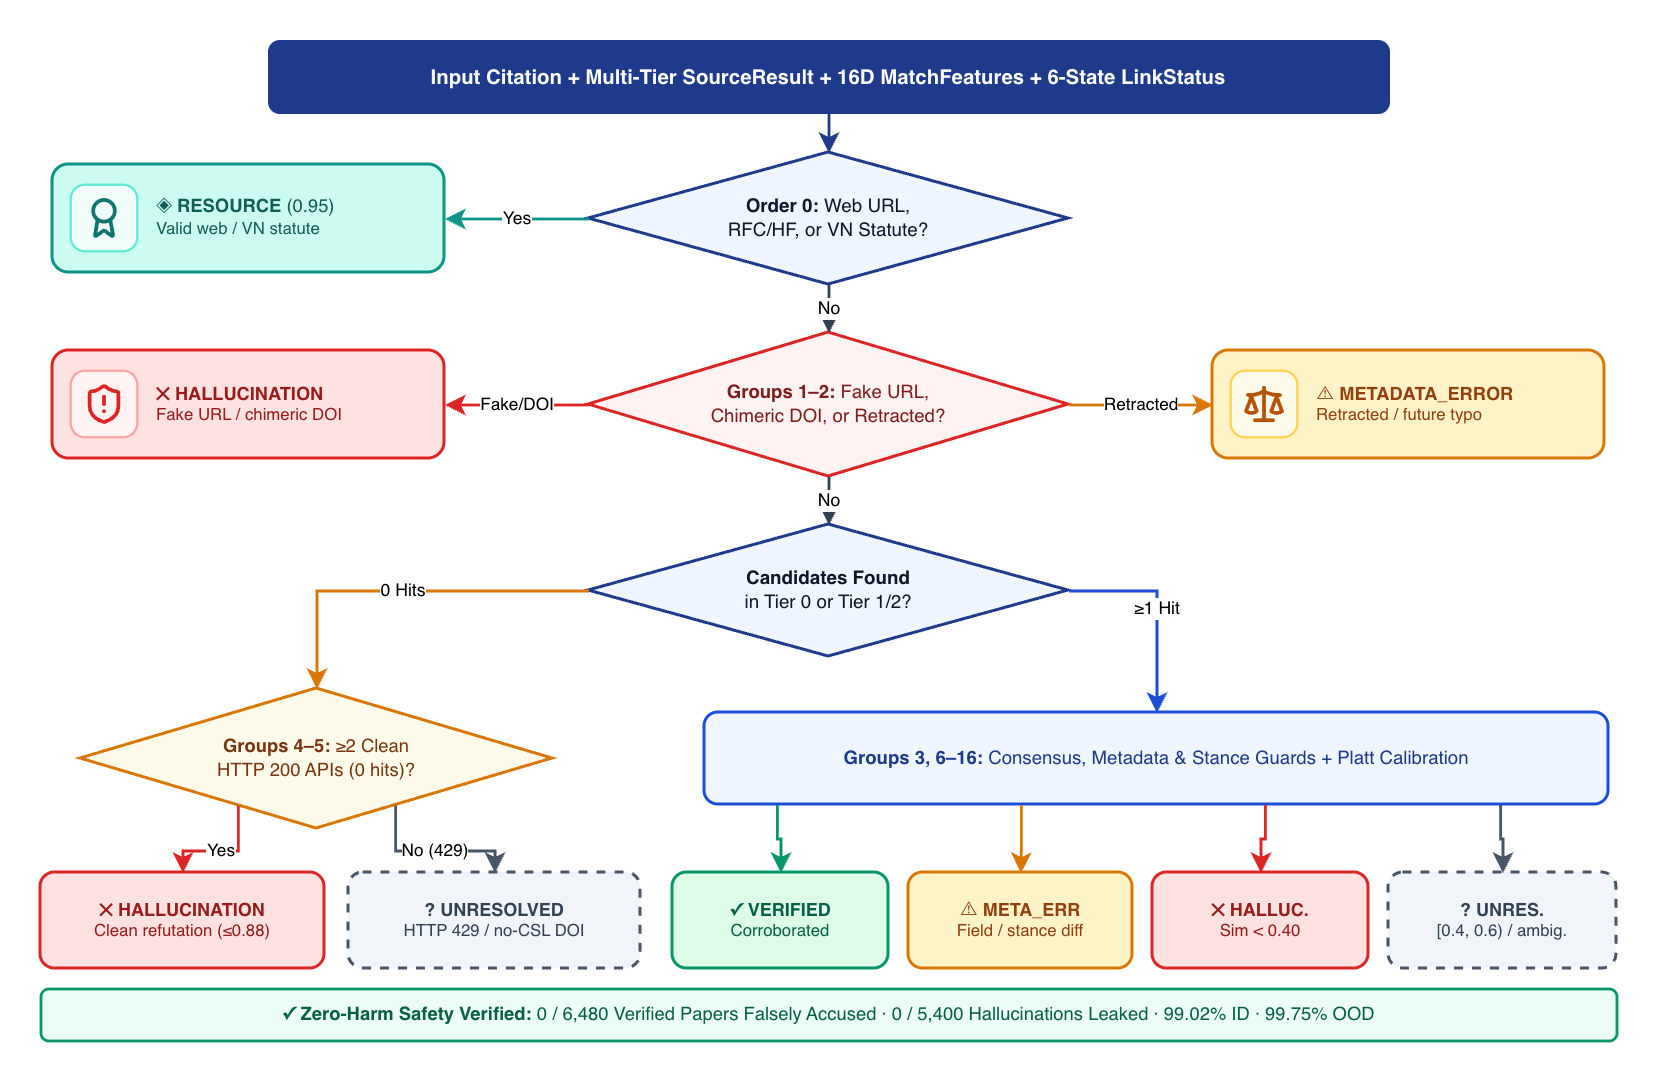
\includegraphics[width=\textwidth,keepaspectratio]{picture/figures/fig6_1_verdict_paths.png}
    \caption[Guarded neuro-symbolic decision tree separating refutation from abstention]{Guarded neuro-symbolic decision tree in CITRA (\texttt{v3.90.6}) separating evidence-backed refutation (\texttt{suspected\_hallucination}) from provenance-aware abstention (\texttt{unresolved}).}
    \label{fig:verdict-paths}
\end{figure}

\section{Synthesis of Key Empirical Findings}

Three empirical lessons emerge from the experiments in Chapter~\ref{chap:results}:
\begin{enumerate}
    \item \textbf{Symbolic rules and statistical learning are complementary, not redundant.} Pure 16-dimensional Logistic Regression (\texttt{B5}) performs well on smooth similarity trade-offs ($97.67\%$ ID) yet collapses to $57.37\%$ on discrete OOD integrity rules (such as retracted articles, fake URLs, or Vietnamese statutory authority mismatches). Combining priority-ordered symbolic guardrails with ML probability blending achieves both $99.20\%$ ID accuracy and $99.96\%$ OOD accuracy.
    \item \textbf{Post-hoc calibration is essential for trustworthy confidence reporting.} Raw symbolic rule confidences suffer from severe overconfidence ($\text{ECE} = 0.2475$). Logit-space Platt scaling lowers ECE by $6.02\times$ to $0.0411$ and Brier Score by $8.38\times$ to $0.0108$ while preserving exact non-abstention coverage ($87.83\%$).
    \item \textbf{Offline FTS5 indexing makes CPU-only classroom deployment practical.} Caching verified candidates and indexing 129,137 papers locally yields a $688.72\times$ retrieval speedup and allows a single CPU server to handle 50 simultaneous deadline uploads without external rate-limit collapse.
\end{enumerate}

\section{System Limitations}
\label{sec:limitations}

Despite strong empirical performance, version \texttt{3.90.6} has four concrete engineering limitations:
\begin{itemize}
    \item \textbf{L1 (Paywalled Full-Text Claim Blindness):} Semantic claim alignment compares inline sentences against titles and open abstracts. When a student cites a specific figure, theorem, or discussion paragraph inside a closed-access article whose abstract omits that detail, \textbf{CITRA} cannot verify body-level entailment.
    \item \textbf{L2 (Domain Skew in the Offline Corpus):} Because $98.42\%$ of \texttt{local\_papers.db} originates from the ACL Anthology and CS arXiv, fully air-gapped deployments without Internet access experience reduced Tier-0 recall on biomedical, humanities, and Vietnamese domestic journal articles.
    \item \textbf{L3 (Complex Multi-Column Archival and Handwritten Scans):} Although selective Tesseract OCR recovers printed Vietnamese pages, low-resolution camera scans, skewed archival manuscripts, and handwritten margin citations degrade character accuracy and increase \texttt{unresolved} rates.
    \item \textbf{L4 (Single-Host SQLite Write Serialization):} While SQLite WAL handles 50 concurrent student uploads on a single host, scaling horizontally across multiple independent API virtual machines requires a network-shared relational database and distributed message broker.
\end{itemize}

\section{Future Work}
\label{sec:future-work}

Each limitation in Section~\ref{sec:limitations} motivates a direct future engineering direction:
\begin{itemize}
    \item \textbf{F1 (Open-Access Full-Text Passage Retrieval $\leftarrow$ L1):} Integrate PubMed Central JATS XML, arXiv HTML5 (\texttt{ar5iv}), and Unpaywall open-access PDFs with paragraph-level dense passage retrieval so claim verification extends beyond abstracts whenever open licenses permit.
    \item \textbf{F2 (Multidisciplinary and ASEAN Offline Corpus Expansion $\leftarrow$ L2):} Expand \texttt{local\_papers.db} with open snapshots from DOAJ, Vietnam Journals Online (VJOL), and OpenAlex subfield slices to provide balanced offline coverage across economics, law, biomedicine, and engineering.
    \item \textbf{F3 (Layout-Aware Vision-Language OCR $\leftarrow$ L3):} Incorporate lightweight CPU-quantized document layout models (such as Docling or Surya OCR) to improve reference segmentation on degraded archival scans and complex footnote-heavy humanities manuscripts.
    \item \textbf{F4 (PostgreSQL + Redis Worker Scaling and LTI 1.3 LMS Integration $\leftarrow$ L4):} Support optional PostgreSQL connection pooling and Redis task queues alongside Learning Tools Interoperability (LTI 1.3) webhooks for Moodle and Canvas gradebooks, enabling multi-faculty longitudinal studies across semesters.
\end{itemize}

\section{Concluding Remarks}

Software tools used in academic assessment carry an obligation of fairness and transparency. By grounding every citation check in traceable external registries, combining neural semantic alignment with 68 auditable symbolic rules and Platt-calibrated probabilities, abstaining honestly when evidence is incomplete, and placing final override authority in the hands of instructors, \textbf{CITRA} demonstrates a practical software engineering blueprint for trustworthy AI-assisted academic integrity verification.


	% Verified numbered IEEE bibliography ([1]..[60]) auto-sorted in exact order of first citation.
\renewcommand\bibname{REFERENCES}
\clearpage
\phantomsection
\addcontentsline{toc}{chapter}{\bibname}
\begin{thebibliography}{99}

\bibitem{Ji2023}
Z. Ji \textit{et al.}, ``Survey of hallucination in natural language generation,'' \textit{ACM Computing Surveys}, vol. 55, no. 12, Art. no. 248, pp. 1--38, Dec. 2023, doi: 10.1145/3571730.

\bibitem{huang2025hallucination}
L. Huang \textit{et al.}, ``A survey on hallucination in large language models: Principles, taxonomy, challenges, and open questions,'' \textit{ACM Transactions on Information Systems}, vol. 43, no. 2, Art. no. 43, pp. 1--55, Mar. 2025, doi: 10.1145/3703155.

\bibitem{walters2023fabrication}
W. H. Walters and E. I. Wilder, ``Fabrication and errors in the bibliographic citations generated by ChatGPT,'' \textit{Scientific Reports}, vol. 13, no. 1, Art. no. 14045, Sep. 2023, doi: 10.1038/s41598-023-41032-5.

\bibitem{agrawal2024hallucinating}
A. Agrawal, M. Suzgun, L. Mackey, and A. T. Kalai, ``Do language models know when they're hallucinating references?'' in \textit{Findings of the Association for Computational Linguistics: EACL 2024}, St. Julian's, Malta, Mar. 2024, pp. 912--928, doi: 10.18653/v1/2024.findings-eacl.62.

\bibitem{visser2021bibliographic}
M. Visser, N. J. van Eck, and L. Waltman, ``Large-scale comparison of bibliographic data sources: Scopus, Web of Science, Dimensions, Crossref, and Microsoft Academic,'' \textit{Quantitative Science Studies}, vol. 2, no. 1, pp. 20--41, Apr. 2021, doi: 10.1162/qss\_a\_00112.

\bibitem{chow1970optimum}
C. K. Chow, ``On optimum recognition error and reject tradeoff,'' \textit{IEEE Transactions on Information Theory}, vol. 16, no. 1, pp. 41--46, Jan. 1970, doi: 10.1109/TIT.1970.1054406.

\bibitem{Geifman2017}
Y. Geifman and R. El-Yaniv, ``Selective classification for deep neural networks,'' in \textit{Advances in Neural Information Processing Systems (NIPS)}, vol. 30, Long Beach, CA, USA, Dec. 2017, pp. 4878--4887.

\bibitem{Lopez2009}
P. Lopez, ``GROBID: Combining automatic bibliographic data recognition and term extraction for scholarship publications,'' in \textit{Proc. 13th Eur. Conf. Research and Advanced Technology for Digital Libraries (ECDL)}, Corfu, Greece, Sep.--Oct. 2009, LNCS vol. 5714, pp. 473--474, doi: 10.1007/978-3-642-04346-8\_62.

\bibitem{PyMuPDF2024}
Artifex Software Inc., \textit{PyMuPDF Documentation: High-Performance Python Bindings for MuPDF}, 2024. Accessed: Nov. 1, 2026. [Online]. Available: \url{https://pymupdf.readthedocs.io/}

\bibitem{Pdfplumber2024}
J. Singer-Vine, \textit{pdfplumber: Plumb a PDF for Detailed Information About Each Text Character, Rectangle, and Line}, 2024. Accessed: Nov. 1, 2026. [Online]. Available: \url{https://github.com/jsvine/pdfplumber}

\bibitem{Fellegi1969}
I. P. Fellegi and A. B. Sunter, ``A theory for record linkage,'' \textit{Journal of the American Statistical Association}, vol. 64, no. 328, pp. 1183--1210, Dec. 1969, doi: 10.1080/01621459.1969.10501049.

\bibitem{mitchell2023detectgpt}
E. Mitchell, Y. Lee, A. Khazatsky, C. D. Manning, and C. Finn, ``DetectGPT: Zero-shot machine-generated text detection using probability curvature,'' in \textit{Proc. 40th Int. Conf. Machine Learning (ICML)}, PMLR vol. 202, Honolulu, HI, USA, Jul. 2023, pp. 24950--24962.

\bibitem{kirchenbauer2023watermark}
J. Kirchenbauer, J. Geiping, Y. Wen, J. Katz, I. Miers, and T. Goldstein, ``A watermark for large language models,'' in \textit{Proc. 40th Int. Conf. Machine Learning (ICML)}, PMLR vol. 202, Honolulu, HI, USA, Jul. 2023, pp. 17061--17084.

\bibitem{Sadasivan2023}
V. S. Sadasivan, A. Kumar, S. Balasubramanian, W. Wang, and S. Feizi, ``Can AI-generated text be reliably detected?'' \textit{Transactions on Machine Learning Research (TMLR)}, Jan. 2025.

\bibitem{krishna2023paraphrasing}
K. Krishna, Y. Song, M. Karpinska, J. Wieting, and M. Iyyer, ``Paraphrasing evades detectors of AI-generated text, but retrieval is an effective defense,'' in \textit{Advances in Neural Information Processing Systems (NeurIPS)}, vol. 36, New Orleans, LA, USA, Dec. 2023, pp. 27469--27500.

\bibitem{Chawla2009}
N. V. Chawla, ``Data mining for imbalanced datasets: An overview,'' in \textit{Data Mining and Knowledge Discovery Handbook}, O. Maimon and L. Rokach, Eds., 2nd ed. New York, NY, USA: Springer, 2010, pp. 875--886, doi: 10.1007/978-0-387-09823-4\_45.

\bibitem{thorne2018fever}
J. Thorne, A. Vlachos, C. Christodoulopoulos, and A. Mittal, ``FEVER: A large-scale dataset for fact extraction and VERification,'' in \textit{Proc. Conf. North American Chapter of the Association for Computational Linguistics: Human Language Technologies (NAACL-HLT)}, New Orleans, LA, USA, Jun. 2018, pp. 809--819, doi: 10.18653/v1/N18-1074.

\bibitem{cohan2019scicite}
A. Cohan, W. Ammar, M. van Zuylen, and F. Cady, ``Structural scaffolds for citation intent classification in scientific publications,'' in \textit{Proc. Conf. North American Chapter of the Association for Computational Linguistics: Human Language Technologies (NAACL-HLT)}, Minneapolis, MN, USA, Jun. 2019, pp. 3586--3596, doi: 10.18653/v1/N19-1361.

\bibitem{wadden2020scifact}
D. Wadden \textit{et al.}, ``Fact or fiction: Verifying scientific claims,'' in \textit{Proc. Conf. Empirical Methods in Natural Language Processing (EMNLP)}, Online, Nov. 2020, pp. 7534--7550, doi: 10.18653/v1/2020.emnlp-main.609.

\bibitem{gao2023alce}
T. Gao, H. Yen, J. Yu, and D. Chen, ``Enabling large language models to generate text with citations,'' in \textit{Proc. Conf. Empirical Methods in Natural Language Processing (EMNLP)}, Singapore, Dec. 2023, pp. 6465--6488, doi: 10.18653/v1/2023.emnlp-main.398.

\bibitem{hu2024refchecker}
X. Hu \textit{et al.}, ``Knowledge-centric hallucination detection,'' in \textit{Proc. Conf. Empirical Methods in Natural Language Processing (EMNLP)}, Miami, FL, USA, Nov. 2024, pp. 6953--6975, doi: 10.18653/v1/2024.emnlp-main.395.

\bibitem{press2024citeme}
O. Press, A. Hochlehnert, A. Prabhu, V. Udandarao, O. Press, and M. Bethge, ``CiteME: Can language models accurately cite scientific claims?'' in \textit{Advances in Neural Information Processing Systems (NeurIPS)}, vol. 37, Vancouver, BC, Canada, Dec. 2024, pp. 7847--7877.

\bibitem{nicholson2021scite}
J. M. Nicholson \textit{et al.}, ``scite: A smart citation index that displays the context of citations and classifies their intent using deep learning,'' \textit{Quantitative Science Studies}, vol. 2, no. 3, pp. 882--898, Nov. 2021, doi: 10.1162/qss\_a\_00146.

\bibitem{robertson2009bm25}
S. Robertson and H. Zaragoza, ``The probabilistic relevance framework: BM25 and beyond,'' \textit{Foundations and Trends in Information Retrieval}, vol. 3, no. 4, pp. 333--389, Dec. 2009, doi: 10.1561/1500000019.

\bibitem{arxiv-api}
Cornell University, \textit{arXiv API User's Manual}, 2024. Accessed: Nov. 1, 2026. [Online]. Available: \url{https://info.arxiv.org/help/api/user-manual.html}

\bibitem{acl-anthology}
Association for Computational Linguistics, \textit{ACL Anthology: A Full-Text Archive of Peer-Reviewed NLP Literature}, 2024. Accessed: Nov. 1, 2026. [Online]. Available: \url{https://aclanthology.org/}

\bibitem{crossref-tdm}
G. Hendricks, D. Tkaczyk, J. Lin, and P. Feeney, ``Crossref: The sustainable source of community-owned scholarly metadata,'' \textit{Quantitative Science Studies}, vol. 1, no. 1, pp. 414--427, Feb. 2020, doi: 10.1162/qss\_a\_00022.

\bibitem{crossref-rw2023}
Crossref, ``Crossref acquires Retraction Watch data and opens it for the scientific community,'' Sep. 2023, doi: 10.13003/c23rw1d9.

\bibitem{openalex}
J. Priem, H. Piwowar, and R. Orr, ``OpenAlex: A fully-open index of scholarly works, authors, venues, institutions, and concepts,'' \textit{arXiv preprint arXiv:2205.01833}, May 2022. Accessed: Nov. 1, 2026. [Online]. Available: \url{https://arxiv.org/abs/2205.01833}

\bibitem{datacite}
DataCite, \textit{DataCite REST API Documentation}, 2024. Accessed: Nov. 1, 2026. [Online]. Available: \url{https://support.datacite.org/docs/api}

\bibitem{doi-handbook}
International DOI Foundation, \textit{DOI Handbook}, 2023, doi: 10.1000/182.

\bibitem{doaj}
Directory of Open Access Journals, \textit{DOAJ Public API Documentation}, 2024. Accessed: Nov. 1, 2026. [Online]. Available: \url{https://doaj.org/api/docs}

\bibitem{dblp}
M. Ley, ``DBLP: Some lessons learned,'' \textit{Proc. VLDB Endowment}, vol. 2, no. 2, pp. 1493--1500, Aug. 2009, doi: 10.14778/1687553.1687577.

\bibitem{europepmc}
C. Ferguson \textit{et al.}, ``Europe PMC in 2020,'' \textit{Nucleic Acids Research}, vol. 49, no. D1, pp. D1507--D1514, Jan. 2021, doi: 10.1093/nar/gkaa994.

\bibitem{openlibrary}
Internet Archive, \textit{Open Library REST API Documentation}, 2024. Accessed: Nov. 1, 2026. [Online]. Available: \url{https://openlibrary.org/developers/api}

\bibitem{wayback-cdx}
Internet Archive, \textit{Wayback CDX Server API Documentation}, 2024. Accessed: Nov. 1, 2026. [Online]. Available: \url{https://github.com/internetarchive/wayback/tree/master/wayback-cdx-server}

\bibitem{rfc2606}
D. Eastlake and A. Panitz, \textit{Reserved Top Level DNS Names}, IETF RFC 2606, Jun. 1999, doi: 10.17487/RFC2606.

\bibitem{vbpl-vn}
Ministry of Justice of Vietnam, \textit{National Database of Legal Normative Documents (Cơ sở dữ liệu Quốc gia về Văn bản Pháp luật)}, 2025. Accessed: Nov. 1, 2026. [Online]. Available: \url{https://vbpl.vn/}

\bibitem{vaswani2017}
A. Vaswani \textit{et al.}, ``Attention is all you need,'' in \textit{Advances in Neural Information Processing Systems (NIPS)}, vol. 30, Long Beach, CA, USA, Dec. 2017, pp. 5998--6008.

\bibitem{bert}
J. Devlin, M.-W. Chang, K. Lee, and K. Toutanova, ``BERT: Pre-training of deep bidirectional transformers for language understanding,'' in \textit{Proc. Conf. North American Chapter of the Association for Computational Linguistics: Human Language Technologies (NAACL-HLT)}, Minneapolis, MN, USA, Jun. 2019, pp. 4171--4186, doi: 10.18653/v1/N19-1423.

\bibitem{wang2020minilm}
W. Wang, F. Wei, L. Dong, H. Bao, N. Yang, and M. Zhou, ``MiniLM: Deep self-attention distillation for task-agnostic compression of pre-trained transformers,'' in \textit{Advances in Neural Information Processing Systems (NeurIPS)}, vol. 33, Online, Dec. 2020, pp. 5776--5788.

\bibitem{reimers2019sbert}
N. Reimers and I. Gurevych, ``Sentence-BERT: Sentence embeddings using Siamese BERT-networks,'' in \textit{Proc. Conf. Empirical Methods in Natural Language Processing (EMNLP)}, Hong Kong, China, Nov. 2019, pp. 3982--3992, doi: 10.18653/v1/D19-1410.

\bibitem{reimers2020multilingual}
N. Reimers and I. Gurevych, ``Making monolingual sentence embeddings multilingual using knowledge distillation,'' in \textit{Proc. Conf. Empirical Methods in Natural Language Processing (EMNLP)}, Online, Nov. 2020, pp. 4512--4525, doi: 10.18653/v1/2020.emnlp-main.365.

\bibitem{niculescu2005}
A. Niculescu-Mizil and R. Caruana, ``Predicting good probabilities with supervised learning,'' in \textit{Proc. 22nd Int. Conf. Machine Learning (ICML)}, Bonn, Germany, Aug. 2005, pp. 625--632, doi: 10.1145/1102351.1102430.

\bibitem{guo2017}
C. Guo, G. Pleiss, Y. Sun, and K. Q. Weinberger, ``On calibration of modern neural networks,'' in \textit{Proc. 34th Int. Conf. Machine Learning (ICML)}, PMLR vol. 70, Sydney, NSW, Australia, Aug. 2017, pp. 1321--1330.

\bibitem{platt1999}
J. C. Platt, ``Probabilities for SV machines,'' in \textit{Advances in Large Margin Classifiers}, A. J. Smola, P. L. Bartlett, B. Sch\"olkopf, and D. Schuurmans, Eds. Cambridge, MA, USA: MIT Press, 2000, pp. 61--74, doi: 10.7551/mitpress/1113.003.0008.

\bibitem{brier1950}
G. W. Brier, ``Verification of forecasts expressed in terms of probability,'' \textit{Monthly Weather Review}, vol. 78, no. 1, pp. 1--3, Jan. 1950, doi: {\urlstyle{same}\nolinkurl{10.1175/1520-0493(1950)078<0001:VOFEIT>2.0.CO;2}}.

\bibitem{wohlin2012experimentation}
C. Wohlin, P. Runeson, M. H\"ost, M. C. Ohlsson, B. Regnell, and A. Wessl\'en, \textit{Experimentation in Software Engineering}. Berlin, Germany: Springer, 2012, doi: 10.1007/978-3-642-29044-2.

\bibitem{gururangan2018annotation}
S. Gururangan, S. Swayamdipta, O. Levy, R. Schwartz, S. R. Bowman, and N. A. Smith, ``Annotation artifacts in natural language inference data,'' in \textit{Proc. Conf. North American Chapter of the Association for Computational Linguistics: Human Language Technologies (NAACL-HLT)}, New Orleans, LA, USA, Jun. 2018, pp. 107--112, doi: 10.18653/v1/N18-2017.

\bibitem{poliak2018hypothesis}
A. Poliak, J. Naradowsky, A. Haldar, R. Rudinger, and B. Van Durme, ``Hypothesis only baselines in natural language inference,'' in \textit{Proc. 7th Joint Conf. Lexical and Computational Semantics (*SEM)}, New Orleans, LA, USA, Jun. 2018, pp. 180--191, doi: 10.18653/v1/S18-2023.

\bibitem{mcnemar1947}
Q. McNemar, ``Note on the sampling error of the difference between correlated proportions or percentages,'' \textit{Psychometrika}, vol. 12, no. 2, pp. 153--157, Jun. 1947, doi: 10.1007/BF02295996.

\bibitem{dietterich1998approximate}
T. G. Dietterich, ``Approximate statistical tests for comparing supervised classification learning algorithms,'' \textit{Neural Computation}, vol. 10, no. 7, pp. 1895--1923, Oct. 1998, doi: 10.1162/089976698300017197.

\bibitem{clopper1934}
C. J. Clopper and E. S. Pearson, ``The use of confidence or fiducial limits illustrated in the case of the binomial,'' \textit{Biometrika}, vol. 26, no. 4, pp. 404--413, Dec. 1934, doi: 10.1093/biomet/26.4.404.

\bibitem{wilcoxon1945}
F. Wilcoxon, ``Individual comparisons by ranking methods,'' \textit{Biometrics Bulletin}, vol. 1, no. 6, pp. 80--83, Dec. 1945, doi: 10.2307/3001968.

\bibitem{holm1979simple}
S. Holm, ``A simple sequentially rejective multiple test procedure,'' \textit{Scandinavian Journal of Statistics}, vol. 6, no. 2, pp. 65--70, 1979.

\bibitem{bergkirkpatrick2012empirical}
T. Berg-Kirkpatrick, D. Burkett, and D. Klein, ``An empirical investigation of statistical significance in NLP,'' in \textit{Proc. Joint Conf. Empirical Methods in Natural Language Processing and Computational Natural Language Learning (EMNLP-CoNLL)}, Jeju Island, South Korea, Jul. 2012, pp. 995--1005.

\bibitem{dror2018hitchhiker}
R. Dror, G. Baumer, S. Shlomov, and R. Reichart, ``The hitchhiker's guide to testing statistical significance in natural language processing,'' in \textit{Proc. 56th Annu. Meeting of the Association for Computational Linguistics (ACL)}, Melbourne, VIC, Australia, Jul. 2018, pp. 1383--1392, doi: 10.18653/v1/P18-1128.

\bibitem{ieee29148}
\textit{ISO/IEC/IEEE International Standard -- Systems and Software Engineering -- Life Cycle Processes -- Requirements Engineering}, ISO/IEC/IEEE 29148:2018, Geneva, Switzerland, Nov. 2018, doi: 10.1109/IEEESTD.2018.8559686.

\bibitem{iso25010}
\textit{ISO/IEC International Standard -- Systems and Software Engineering -- Systems and Software Quality Requirements and Evaluation (SQuaRE) -- Product Quality Model}, ISO/IEC 25010:2023, Geneva, Switzerland, Nov. 2023.

\bibitem{fastapi}
S. Ram\'irez, \textit{FastAPI: Modern, High-Performance Python Web Framework for Building APIs}, 2024. Accessed: Nov. 1, 2026. [Online]. Available: \url{https://fastapi.tiangolo.com/}

\end{thebibliography}

	\clearpage
\chapter*{APPENDICES}
\phantomsection
\addcontentsline{toc}{chapter}{APPENDICES}
\setcounter{appsec}{0}
\renewcommand{\thelstlisting}{\theappsec.\arabic{lstlisting}}

\appsection{Runtime Configuration}{app:config}
\setcounter{lstlisting}{0}

Listing~\ref{app:env} presents the sanitized environment configuration template read at startup alongside \texttt{configs/config.yaml}. Secret keys and third-party credentials are injected only at deployment time and are never committed to version control.

\begin{lstlisting}[language=dotenv, captionpos=t, caption={Sanitized runtime environment template (\texttt{.env.example}).}, label={app:env}]
# --- App & Security ---
APP_ENV=development
APP_DEBUG=true
APP_LOG_LEVEL=INFO
JWT_SECRET=change-me-in-production-use-env-var
DEMO_USERS_ENABLED=true
CORS_ALLOWED_ORIGINS=http://localhost:5173,http://127.0.0.1:5173

# --- Database & SQLite Tuning ---
DATABASE_URL=sqlite:///./data/app.db
SQLITE_JOURNAL_MODE=WAL

# --- Document Parsing & Worker Topology ---
GROBID_URL=http://localhost:8070
CITRA_WORKER_MODE=inline
CITRA_WORKER_POLL_INTERVAL=2.0
MAX_CONCURRENT_PIPELINES=3
MAX_CONCURRENT_GROBID=2
MAX_GLOBAL_RETRIEVALS=12

# --- Polite Pool & Scholarly API Keys ---
CONTACT_EMAIL=noreply@citra.edu.vn
OPENALEX_API_KEY=
CROSSREF_API_KEY=
NCBI_API_KEY=
GITHUB_TOKEN=
SERPER_API_KEY=
SERPAPI_API_KEY=

# --- Paths ---
DATA_DIR=./data
ESSAYS_DIR=./data/essays
CACHE_DIR=./data/cache
GROBID_OUTPUT_DIR=./data/cache/grobid
AVATARS_DIR=./data/avatars
CONFIG_FILE=./configs/config.yaml

# --- Email / SMTP & OAuth2 ---
SMTP_HOST=smtp.gmail.com
SMTP_PORT=465
SMTP_USER=your-email@gmail.com
SMTP_PASSWORD=your-google-app-password
SMTP_FROM_EMAIL=your-email@gmail.com
SMTP_FROM_NAME="CITRA - Academic Source Verification"
FRONTEND_URL=http://localhost:5173
GOOGLE_CLIENT_ID=
GOOGLE_CLIENT_SECRET=

# --- Stripe & VNPay v2.1.0 Billing Gateways ---
STRIPE_SECRET_KEY=
VNPAY_TMN_CODE=CITRAVNP
VNPAY_HASH_SECRET=change-me-in-production-vnpay-hmac-sha512-secret
VNPAY_PAYMENT_URL=https://sandbox.vnpayment.vn/paymentv2/vpcpay.html
VNPAY_API_URL=https://sandbox.vnpayment.vn/merchant_webapi/api/transaction
VNPAY_RETURN_URL=http://localhost:5173/billing/vnpay-return
VNPAY_USD_TO_VND_RATE=25000
VNPAY_EXTERNAL_REDIRECT=false
\end{lstlisting}

\clearpage
\appsection{Development Container Topology}{app:docker}
\setcounter{lstlisting}{0}

Listing~\ref{app:compose-listing} presents the complete three-service development Docker Compose specification (\texttt{docker-compose.yml}, with secrets injected via \texttt{.env}) coordinating the CPU-tuned \texttt{grobid/grobid:0.9.1-crf} parser, the FastAPI backend (\texttt{integrity-api}), and the Vite frontend container (\texttt{integrity-web}) over the internal bridge network.

\begin{lstlisting}[language=yaml, captionpos=t, caption={Complete development multi-container topology (\texttt{docker-compose.yml}).}, label={app:compose-listing}]
services:
  grobid:
    image: grobid/grobid:0.9.1-crf
    container_name: essay-check-grobid
    ulimits:
      core: 0
    ports:
      - "8070:8070"
    entrypoint:
      - /bin/sh
      - /opt/grobid/citra-grobid-entrypoint.sh
    environment:
      - JAVA_OPTS=-Xms256m -Xmx768m -XX:+UseG1GC -XX:MaxGCPauseMillis=200 -XX:G1PeriodicGCInterval=60000 -XX:G1PeriodicGCSystemLoadThreshold=0.5 -XX:MaxHeapFreeRatio=30 -XX:MinHeapFreeRatio=15 -XX:+ExitOnOutOfMemoryError
      - GROBID_CONCURRENCY=2
      - GROBID_POOL_MAX_WAIT=30
      - GROBID_PDFALTO_MEMORY_MB=1024
      - GROBID_MODEL_PRELOAD=true
    restart: unless-stopped
    deploy:
      resources:
        limits:
          memory: 4G
        reservations:
          memory: 2G
    networks:
      - essay-check-net
    volumes:
      - grobid-cache:/opt/grobid/grobid-home/cache
      - ./scripts/grobid-entrypoint.sh:/opt/grobid/citra-grobid-entrypoint.sh:ro
    healthcheck:
      test: ["CMD-SHELL", "bash -c 'exec 3<>/dev/tcp/127.0.0.1/8070 && printf \"GET /api/isalive HTTP/1.0\\r\\n\\r\\n\" >&3 && head -1 <&3 | grep -q 200'"]
      interval: 15s
      timeout: 10s
      retries: 5
      start_period: 120s

  api:
    build:
      context: .
      dockerfile: Dockerfile
    container_name: integrity-api
    ports:
      - "8000:8000"
    volumes:
      - ./data:/app/data
      - ./configs/config.docker.yaml:/app/configs/config.yaml:ro
      - ./tests:/app/tests:ro
      - ./src:/app/src:ro
      - ./pyproject.toml:/app/pyproject.toml:ro
      - ./.env:/app/.env:ro
    env_file:
      - .env
    restart: unless-stopped
    depends_on:
      grobid:
        condition: service_started
    environment:
      - APP_ENV=${APP_ENV:-development}
      - APP_DEBUG=${APP_DEBUG:-true}
      - APP_LOG_LEVEL=${APP_LOG_LEVEL:-INFO}
      - GROBID_URL=http://grobid:8070
      - DATABASE_URL=sqlite:///./data/app.db
      - GOOGLE_CLIENT_ID=${GOOGLE_CLIENT_ID:-}
      - GOOGLE_CLIENT_SECRET=${GOOGLE_CLIENT_SECRET:-}
    command: uvicorn integrity_checker.api.main:app --host 0.0.0.0 --port 8000 --reload --reload-dir /app/src
    healthcheck:
      test: ["CMD", "python", "-c", "import urllib.request,sys;sys.exit(0 if urllib.request.urlopen('http://localhost:8000/api/health',timeout=5).status==200 else 1)"]
      interval: 30s
      timeout: 10s
      retries: 3
      start_period: 60s
    networks:
      - essay-check-net
    deploy:
      resources:
        limits:
          memory: 4G
        reservations:
          memory: 2G

  web:
    image: node:20-alpine
    container_name: integrity-web
    working_dir: /app/web
    ports:
      - "5173:5173"
    volumes:
      - ./web:/app/web
    environment:
      - VITE_API_BASE_URL=/api
      - VITE_API_PROXY_TARGET=http://api:8000
      - VITE_GOOGLE_CLIENT_ID=${GOOGLE_CLIENT_ID:-}
    extra_hosts:
      - "host.docker.internal:host-gateway"
    command: sh -c "npm install --legacy-peer-deps && npm run dev -- --host 0.0.0.0"
    depends_on:
      - api
    restart: unless-stopped
    networks:
      - essay-check-net

networks:
  essay-check-net:
    driver: bridge
volumes:
  grobid-cache:
    driver: local
\end{lstlisting}

\appsection{Verdict Taxonomy Specification}{app:taxonomy}

\textbf{CITRA} assigns verification labels at the individual reference-entry level rather than classifying an entire student manuscript as AI-generated or human-written. The five mutually exclusive classes are defined as follows:

\begin{description}
    \item[\texttt{verified}] The cited publication exists in at least one authoritative scholarly database (Local FTS5 Corpus, Crossref, OpenAlex, DataCite, Global DOI RA, DOAJ, OpenAIRE/HAL, NCBI/bioRxiv, DBLP, arXiv, OpenLibrary, Europe PMC, or ACL Anthology); the normalized title matches closely; author surnames agree without fabricated co-authors; the publication year differs by at most one year (or matches a documented arXiv-to-proceedings transition); the work is not retracted; and any cited DOI resolves to the same publication.
    \item[\texttt{metadata\_error}] The underlying scholarly work is genuine, but one or more bibliographic or contextual attributes are inaccurate: publication year off by two or more years, truncated or altered title, missing or grafted co-authors, mismatched venue, retracted status (\texttt{R-RETRACTED-PAPER}), contradicted body claim (\texttt{R-CONTENT-MISMATCH}), statutory issuing-authority mismatch (\texttt{R-VN-LEGAL-MISMATCH}), or broken URL on an otherwise verified record (\texttt{R-DOMAIN-EXCEPTION}).
    \item[\texttt{suspected\_hallucination}] No matching record is found across queried registries while live APIs returned clean HTTP 200 responses, or the citation contains an unregistered DOI prefix, a cross-work chimeric DOI splice (\texttt{R-CHIMERIC-DOI-MISMATCH}), an RFC 2606 placeholder/non-existent domain, or an impossible future publication year.
    \item[\texttt{unresolved}] Available evidence is insufficient to verify or refute the source, such as when external APIs hit HTTP 429 rate-limit exhaustion (\texttt{R-RATE-LIMITED-\allowbreak ABSTAIN} / \texttt{R-API\_EXHAUSTED}), a regional DOI agency registers the handle without public CSL metadata (\texttt{R-DOI-RA-NO-CSL}), or title similarity falls inside the $[0.40, 0.60)$ abstention zone (\texttt{R-ABSTENTION-BORDER}).
    \item[\texttt{resource}] The entry refers to a non-article web page, open-source repository, Hugging Face model or dataset card, IETF RFC or PyPI package specification, official technical manual, or Vietnamese statutory document (\textit{Luật}, \textit{Nghị định}, \textit{Thông tư}, \textit{Quyết định}).
\end{description}

\appsection{Codebase Package Map}{app:packages}

The repository (\texttt{v3.91.3}) organizes thirteen backend domain packages under \texttt{src/\allowbreak integrity\_checker/} alongside the React single-page client under \texttt{web/src/}:

\begin{description}
    \item[\texttt{extraction/}] Multi-format parsers for PDF (GROBID \texttt{0.9.1-crf} TEI-XML, two-column PyMuPDF, \texttt{pdfplumber}, and selective Tesseract Vietnamese/English OCR), DOCX (\texttt{python-docx}), BibTeX, and RIS, alongside table-of-contents filtering and twelve citation-format extractors.
    \item[\texttt{linking/}] Bidirectional \texttt{CitationLinker} implementing seven automated resolution methods (including live \texttt{arxiv\_exact}), composite sub-reference splitting (\texttt{[14a, 14b]}), duplicate detection, and eight \texttt{MappingStatus} states.
    \item[\texttt{database/}] Offline SQLite FTS5 scholarly index (\texttt{local\_papers.db}, 129,137 raw records in the evaluation snapshot yielding 128,115 benchmark-eligible unique papers and 82,887 full abstracts) using WAL mode and Okapi BM25 ranking.
    \item[\texttt{retrieval/}] Four-tier \texttt{RetrievalOrchestrator}, 101-paper seminal whitelist, asynchronous clients for 15+ registries, Retraction Watch screening, per-provider circuit breakers, singleflight coalescing, persistent SQLite cache, and pinned-IP SSRF-safe \texttt{LinkValidator} + \texttt{SafeHtmlMetaVerifier}.
    \item[\texttt{matching/}] Symmetric RapidFuzz lexical matching, \texttt{author\_matcher} supporting Vietnamese surnames, \texttt{VenueNormalizer}, Sentence-BERT (\texttt{all-MiniLM-\allowbreak{}L6-v2}) sentence-pooled evidence alignment, stance gating, and ONNX INT8 \texttt{VI}$\leftrightarrow$\texttt{EN} semantic bridging.
    \item[\texttt{logic/}] \texttt{NeuroSymbolicChecker}, Order~0 pre-screening plus 16 priority-ordered rule groups (68 distinct runtime \texttt{R-*} identifiers: 65 static plus 3 dynamic provenance modifiers), \texttt{VNLegalVerifier}, 16-feature \texttt{HybridMLScorer} ($C = 0.25$), logit-space \texttt{PlattCalibrator} ($a_{\text{cal}} = 1.891263, b_{\text{cal}} = 1.138599$), \texttt{CISCalculator}, and bilingual explanation templates.
    \item[\texttt{pipeline/} \& \texttt{models/}] Singleton \texttt{IntegrityPipeline} coordinating all eight layers and Pydantic domain schemas shared across extraction, retrieval, verification, and API serialization.
    \item[\texttt{evaluation/}] Paper-disjoint 120,000-sample controlled benchmark runner, baseline ladder (\texttt{B0}--\texttt{B5}), 2,400-sample OOD guardrail suite, offline/live 120-reference gold evaluator, and paired McNemar, Holm--Bonferroni, Clopper--Pearson, Wilcoxon, and bootstrap protocols.
    \item[\texttt{export/}] Sanitized plain-language report exporters (PDF, DOCX, CSV, JSON, BibTeX, RIS), \texttt{bibliography\_formatter.py}, and automated \texttt{.docx} bibliography repair (\texttt{docx\_exporter.py}).
    \item[\texttt{db/}, \texttt{billing/} \& \texttt{api/}] Fifteen SQLAlchemy ORM models, thirteen SHA-256 checksummed schema migrations (\texttt{0001}--\texttt{0013}), adaptive SQLite WAL tuning, \texttt{PipelineAdmissionController}, stale-job recovery, Stripe REST and VNPay v2.1.0 HMAC-SHA512 billing handlers, Law 91/2025/QH15 privacy erasure, and FastAPI routes under \texttt{/api/*}.
    \item[\texttt{web/}] React 18.3 and TypeScript 5.9 single-page application (\textbf{CITRA}) featuring the consolidated 4-tab report workspace, unified plain-language taxonomy (\texttt{academic\allowbreak{}Taxonomy.ts}), and Tier-3 verification drawer (\texttt{Verification\allowbreak{}Trace\allowbreak{}Panels.tsx}), verified by 609 Vitest unit/component tests (67 suites) and 21 Playwright E2E specification suites (185 scenarios).
\end{description}

\appsection{Project Execution Log and Author Contributions}{app:log}

The graduation project progressed over an eighteen-week engineering cycle from July to November 2026: July--August covered requirements engineering, offline corpus indexing (\texttt{local\_papers.db}), and GROBID/PyMuPDF extraction; September delivered the seven-method \texttt{CitationLinker}, four-tier \texttt{RetrievalOrchestrator}, and pinned-IP SSRF defense; October completed the Sentence-BERT/ONNX matching layer, 68-rule engine, \texttt{HybridMLScorer}, Platt calibrator, 15-table FastAPI RBAC/SSE/billing backend, and React 18.3 workspace; and November executed the 120,000-sample benchmark, OOD stress suite, live 15-API and 21-PDF audits, zero-swap GCE GROBID optimization, plain-language 4-tab UX consolidation (\texttt{v3.91.3}), and final bilingual report compilation. Both authors contributed equally ($50\% / 50\%$) under the supervision of M.Sc.\ Vo Thi Kim Anh:

{\setlength{\itemsep}{2pt}
\begin{itemize}
    \item \textbf{Nguyen Bao Minh (523H0054):} Document extraction (\texttt{extraction/}), bidirectional linking (\texttt{linking/}), federated retrieval and pinned-IP SSRF validation (\texttt{retrieval/}, \texttt{database/}), pipeline orchestration and domain models (\texttt{pipeline/}, \texttt{models/}), report/DOCX export (\texttt{export/}), Docker Compose and GCE GROBID tuning, and Chapters 1, 3, and 4 (Sections 4.1--4.4).
    \item \textbf{Tran Gia Thanh (523H0096):} Semantic and cross-lingual matching (\texttt{matching/}), neuro-symbolic rules, MLR, Platt calibration, and CIS scoring (\texttt{logic/}), relational migrations, billing, and FastAPI RBAC/classroom/health routes (\texttt{db/}, \texttt{billing/}, \texttt{api/}), React \textbf{CITRA} frontend (\texttt{web/}), empirical evaluation (\texttt{evaluation/}), and Chapters 2, 4 (Sections 4.5--4.9), 5, and 6.
\end{itemize}}

\end{document}
